%%%%%%%%%%%%%%%%%%%%%%%%%%%%%%%%%%%%%%%%%
% Masters/Doctoral Thesis 
% LaTeX Template
% Version 2.2.2 (20/2/16)
%
% This template has been downloaded from:
% http://www.LaTeXTemplates.com
%
% Version 2.x major modifications by:
% Vel (vel@latextemplates.com)
%
% This template is based on a template by:
% Steve Gunn (http://users.ecs.soton.ac.uk/srg/softwaretools/document/templates/)
% Sunil Patel (http://www.sunilpatel.co.uk/thesis-template/)
%
% Template license:
% CC BY-NC-SA 3.0 (http://creativecommons.org/licenses/by-nc-sa/3.0/)
%
%%%%%%%%%%%%%%%%%%%%%%%%%%%%%%%%%%%%%%%%%

%----------------------------------------------------------------------------------------
%	PACKAGES AND OTHER DOCUMENT CONFIGURATIONS
%----------------------------------------------------------------------------------------

\documentclass[
11pt, % The default document font size, options: 10pt, 11pt, 12pt
oneside, % Two side (alternating margins) for binding by default, uncomment to switch to one side
english, % ngerman for German
singlespacing, % Single line spacing, alternatives: onehalfspacing or doublespacing
%draft, % Uncomment to enable draft mode (no pictures, no links, overfull hboxes indicated)
%nolistspacing, % If the document is onehalfspacing or doublespacing, uncomment this to set spacing in lists to single
liststotoc, % Uncomment to add the list of figures/tables/etc to the table of contents
%toctotoc, % Uncomment to add the main table of contents to the table of contents
%parskip, % Uncomment to add space between paragraphs
%nohyperref, % Uncomment to not load the hyperref package
headsepline, % Uncomment to get a line under the header
]{MastersDoctoralThesis} % The class file specifying the document structure

\usepackage[utf8]{inputenc} % Required for inputting international characters
\usepackage[T1]{fontenc} % Output font encoding for international characters

\usepackage{palatino} % Use the Palatino font by default

%\usepackage{hyperref}

\usepackage[backend=bibtex,citestyle=phys,natbib=true]{biblatex} % Use the bibtex backend with the authoryear citation style (which resembles APA)

\addbibresource{example.bib} % The filename of the bibliography

\usepackage[autostyle=true]{csquotes} % Required to generate language-dependent quotes in the bibliography

\usepackage{amsmath}
\usepackage{mathtools}

\usepackage{algorithm}
\usepackage{algpseudocode}
\usepackage{pifont}

%\usepackage[usenames,x11names,dvipsnames,svgnames]{xcolor}
%\usepackage{graphicx,amsmath,latexsym,amssymb,amsthm,geometry}
\usepackage{tikz}
%\usepackage{pagecolor}% http://ctan.org/pkg/{pagecolor,lipsum}
\usetikzlibrary{arrows.meta,decorations,decorations.text,backgrounds,arrows,shapes,intersections,calc,hobby}
%\usetikzlibrary{verbatim}

\usepackage{cleveref}

\usepackage{subfigure}

%\usepackage{gensymb}

%\newtheorem{theorem}{Theorem}[section]
%\newtheorem{lemma}[theorem]{Lemma}
%\newtheorem{proposition}[theorem]{Proposition}
%\newtheorem{corollary}[theorem]{Corollary}
%
%\newenvironment{proof}[1][Proof]{\begin{trivlist}
%		\item[\hskip \labelsep {\bfseries #1}]}{\end{trivlist}}
%\newenvironment{definition}[1][Definition]{\begin{trivlist}
%		\item[\hskip \labelsep {\bfseries #1}]}{\end{trivlist}}
%\newenvironment{example}[1][Example]{\begin{trivlist}
%		\item[\hskip \labelsep {\bfseries #1}]}{\end{trivlist}}
%\newenvironment{remark}[1][Remark]{\begin{trivlist}
%		\item[\hskip \labelsep {\bfseries #1}]}{\end{trivlist}}
%
%\newcommand{\qed}{\nobreak \ifvmode \relax \else
%	\ifdim\lastskip<1.5em \hskip-\lastskip
%	\hskip1.5em plus0em minus0.5em \fi \nobreak
%	\vrule height0.75em width0.5em depth0.25em\fi}\newtheorem{theorem}{Theorem}[section]
%\newtheorem{lemma}[theorem]{Lemma}
%\newtheorem{proposition}[theorem]{Proposition}
%\newtheorem{corollary}[theorem]{Corollary}
%
%\newenvironment{proof}[1][Proof]{\begin{trivlist}
%		\item[\hskip \labelsep {\bfseries #1}]}{\end{trivlist}}
\newenvironment{definition}[1][Definition]{\begin{trivlist}
		\item[\hskip \labelsep {\bfseries #1}]}{\end{trivlist}}
%\newenvironment{example}[1][Example]{\begin{trivlist}
%		\item[\hskip \labelsep {\bfseries #1}]}{\end{trivlist}}
%\newenvironment{remark}[1][Remark]{\begin{trivlist}
%		\item[\hskip \labelsep {\bfseries #1}]}{\end{trivlist}}
%
%\newcommand{\qed}{\nobreak \ifvmode \relax \else
%	\ifdim\lastskip<1.5em \hskip-\lastskip
%	\hskip1.5em plus0em minus0.5em \fi \nobreak
%	\vrule height0.75em width0.5em depth0.25em\fi}


%----------------------------------------------------------------------------------------
%	MARGIN SETTINGS
%----------------------------------------------------------------------------------------

\geometry{
	paper=letterpaper, % Change to letterpaper for US letter or a4paper
	inner=2.5cm, % Inner margin
	outer=2.5cm,%3.8cm, % Outer margin
	bindingoffset=2cm, % Binding offset
	top=1.5cm, % Top margin
	bottom=1.5cm, % Bottom margin
	%showframe,% show how the type block is set on the page
}

%----------------------------------------------------------------------------------------
%	THESIS INFORMATION
%----------------------------------------------------------------------------------------

\thesistitle{Discrete Energy Minimisation Optimisation using Graph Cuts for Fluorescence Microscopy} % Your thesis title, this is used in the title and abstract, print it elsewhere with \ttitle
\supervisor{Dr. Jules-Raymond \textsc{Tapamo}} % Your supervisor's name, this is used in the title page, print it elsewhere with \supname
\examiner{} % Your examiner's name, this is not currently used anywhere in the template, print it elsewhere with \examname
\degree{Master of Science in Engineering} % Your degree name, this is used in the title page and abstract, print it elsewhere with \degreename
\author{Ryan \textsc{Naidoo}} % Your name, this is used in the title page and abstract, print it elsewhere with \authorname
\addresses{} % Your address, this is not currently used anywhere in the template, print it elsewhere with \addressname

\subject{Computer Vision} % Your subject area, this is not currently used anywhere in the template, print it elsewhere with \subjectname
\keywords{} % Keywords for your thesis, this is not currently used anywhere in the template, print it elsewhere with \keywordnames
\university{\href{http://www.university.com}{University of KwaZulu-Natal (Howard College)}} % Your university's name and URL, this is used in the title page and abstract, print it elsewhere with \univname
\department{\href{http://department.university.com}{School of Engineering}} % Your department's name and URL, this is used in the title page and abstract, print it elsewhere with \deptname
\group{\href{http://researchgroup.university.com}{Department of Electrical, Electronic and Computer Engineering}} % Your research group's name and URL, this is used in the title page, print it elsewhere with \groupname
\faculty{\href{http://faculty.university.com}{Faculty of Engineering}} % Your faculty's name and URL, this is used in the title page and abstract, print it elsewhere with \facname

\hypersetup{pdftitle=\ttitle} % Set the PDF's title to your title
\hypersetup{pdfauthor=\authorname} % Set the PDF's author to your name
\hypersetup{pdfkeywords=\keywordnames} % Set the PDF's keywords to your keywords

\makeatletter
\newcommand{\addloflink}[1]{% \addloflink{<URL>}
	\addtocontents{lof}{\begingroup\def\protect\@dotsep{10000}% Remove dots in LoF for this entry
		\protect\contentsline{figlink}{\protect\numberline{}\url{#1}}{}{}%
		\endgroup}% Restore dots in LoF for future entries
}
\newcommand{\l@figlink}{\@dottedtocline{1}{1.5em}{2.3em}}
\makeatother

%\captionsetup{width=\columnwidth}

\begin{document}
	
\frontmatter % Use roman page numbering style (i, ii, iii, iv...) for the pre-content pages

\pagestyle{plain} % Default to the plain heading style until the thesis style is called for the body content

%----------------------------------------------------------------------------------------
%	TITLE PAGE
%----------------------------------------------------------------------------------------

\begin{titlepage}
\begin{center}

{\scshape\LARGE \univname\par}\vspace{1.5cm} % University name
\textsc{\Large Masters Thesis}\\[0.5cm] % Thesis type

\HRule \\[0.4cm] % Horizontal line
{\huge \bfseries \ttitle\par}\vspace{0.4cm} % Thesis title
\HRule \\[1.5cm] % Horizontal line
 
\begin{minipage}[t]{0.4\textwidth}
\begin{flushleft} \large
\emph{Author:}\\
\href{http://www.johnsmith.com}{\authorname} % Author name - remove the \href bracket to remove the link
\end{flushleft}
\end{minipage}
\begin{minipage}[t]{0.4\textwidth}
\begin{flushright} \large
\emph{Supervisor:} \\
\href{http://www.jamessmith.com}{\supname} % Supervisor name - remove the \href bracket to remove the link  
\end{flushright}
\end{minipage}\\[3cm]
 
\large \textit{A thesis submitted in fulfillment of the requirements\\ for the degree of \degreename}\\[0.3cm] % University requirement text
\textit{in the}\\[0.4cm]
\groupname\\\deptname\\[2cm] % Research group name and department name
 
{\large \today}\\[4cm] % Date
%
\includegraphics{Logo} % University/department logo - uncomment to place it
 
\vfill
\end{center}
\end{titlepage}

%----------------------------------------------------------------------------------------
%	DECLARATION PAGE
%----------------------------------------------------------------------------------------

\begin{declaration}
\addchaptertocentry{\authorshipname}

\noindent I, \authorname, declare that this thesis titled, \enquote{\ttitle} and the work presented in it are my own. I confirm that:

\begin{itemize} 
\item This work was done wholly or mainly while in candidature for a research degree at this University.
\item Where any part of this thesis has previously been submitted for a degree or any other qualification at this University or any other institution, this has been clearly stated.
\item Where I have consulted the published work of others, this is always clearly attributed.
\item Where I have quoted from the work of others, the source is always given. With the exception of such quotations, this thesis is entirely my own work.
\item I have acknowledged all main sources of help.
\item Where the thesis is based on work done by myself jointly with others, I have made clear exactly what was done by others and what I have contributed myself.\\
\end{itemize}
 
\noindent Signed:\\
\rule[0.5em]{25em}{0.5pt} % This prints a line for the signature
 
\noindent Date:\\
\rule[0.5em]{25em}{0.5pt} % This prints a line to write the date
\end{declaration}

\cleardoublepage

%----------------------------------------------------------------------------------------
%	QUOTATION PAGE
%----------------------------------------------------------------------------------------

\vspace*{0.2\textheight}

\noindent\enquote{\itshape Thanks to my solid academic training, today I can write hundreds of words on virtually any topic without possessing a shred of information, which is how I got a good job in journalism.}\bigbreak

\hfill Dave Barry

%----------------------------------------------------------------------------------------
%	ABSTRACT PAGE
%----------------------------------------------------------------------------------------

\begin{abstract}
\addchaptertocentry{\abstractname} % Add the abstract to the table of contents

The Thesis Abstract is written here (and usually kept to just this page). The page is kept centered vertically so can expand into the blank space above the title too\ldots

\end{abstract}

%----------------------------------------------------------------------------------------
%	ACKNOWLEDGEMENTS
%----------------------------------------------------------------------------------------

\begin{acknowledgements}
\addchaptertocentry{\acknowledgementname} % Add the acknowledgements to the table of contents

The acknowledgments and the people to thank go here, don't forget to include your project advisor\ldots

\end{acknowledgements}

%----------------------------------------------------------------------------------------
%	LIST OF CONTENTS/FIGURES/TABLES PAGES
%----------------------------------------------------------------------------------------

\tableofcontents % Prints the main table of contents

\listoffigures % Prints the list of figures

\listoftables % Prints the list of tables

\listofalgorithms % Prints the list of algorithms

%----------------------------------------------------------------------------------------
%	ABBREVIATIONS
%----------------------------------------------------------------------------------------

\begin{abbreviations}{ll} % Include a list of abbreviations (a table of two columns)

% A
\textbf{ACWE} & \textbf{A}ctive \textbf{C}ontours \textbf{W}ithout \textbf{E}dges\\

% B
% C
\textbf{CED} & \textbf{C}oherence \textbf{E}nhancing \textbf{D}iffusion\\
\textbf{CCD} & \textbf{C}harge-\textbf{C}oupled \textbf{D}evice\\
\textbf{CLSM} & \textbf{C}onfocal \textbf{L}aser \textbf{S}canning \textbf{M}icroscopy\\
\textbf{CRF} & \textbf{C}onditional \textbf{R}andom \textbf{F}ield\\

% D
\textbf{DNA} & \textbf{D}eoxyribo\textbf{n}ucleic \textbf{A}cid\\

% E
\textbf{EGFP} & \textbf{E}nhanced \textbf{G}reen \textbf{F}luorescent \textbf{P}rotein\\
\textbf{EM} & \textbf{E}xpectation \textbf{M}aximisation\\

% F
\textbf{FCS} & \textbf{F}luorenscence \textbf{C}orrelation \textbf{S}pectroscopy\\
\textbf{FIFO} & \textbf{F}irst-\textbf{I}n \textbf{F}irst-\textbf{O}ut\\
\textbf{FISH} & \textbf{F}luorenscence \textbf{i}n-\textbf{s}itu \textbf{H}ybridisation\\
\textbf{FLIM} & \textbf{F}luorenscence \textbf{L}ifetime \textbf{I}maging \textbf{M}icroscopy\\
\textbf{FRAP} & \textbf{F}luorenscence \textbf{R}ecovery \textbf{A}fter \textbf{P}hotobleaching\\
\textbf{FRET} & \textbf{F}luorenscence \textbf{R}esonance \textbf{E}nergy \textbf{T}ransfer\\

% G
\textbf{GFP} & \textbf{G}reen \textbf{F}luorescent \textbf{P}rotein\\
\textbf{GMM} & \textbf{G}uassian \textbf{M}ixture \textbf{M}odelling\\

% H
% I
\textbf{ICC} & \textbf{I}mmuno\textbf{c}yto\textbf{c}hemistry\\
\textbf{ICF} & \textbf{I}mmuno\textbf{c}yto\textbf{f}luorescence\\
\textbf{IHC} & \textbf{I}mmuno\textbf{h}isto\textbf{c}hemistry\\
\textbf{IHF} & \textbf{I}mmuno\textbf{h}isto\textbf{f}luorescence\\

% J
% K
% L
\textbf{LED} & \textbf{L}ight \textbf{E}mitting \textbf{D}iode\\

% M
\textbf{MAP} & \textbf{M}aximum \textbf{A} \textbf{P}osteriori\\
\textbf{MIS} & \textbf{M}edical \textbf{I}mage \textbf{S}egmentation\\
\textbf{MLP} & \textbf{M}ulti-\textbf{L}ayered \textbf{P}erceptron\\
\textbf{MRF} & \textbf{M}arkov \textbf{R}andom \textbf{F}ield\\

% N
\textbf{NA} & \textbf{N}umerical \textbf{A}perture\\

% O
\textbf{ORI} & \textbf{O}ptimised \textbf{R}otational \textbf{I}nvariance\\

% P
\textbf{PSF} & \textbf{P}oint \textbf{S}pread \textbf{F}unction\\

% Q
% R
\textbf{RNA} & \textbf{R}ibo\textbf{n}ucleic \textbf{A}cid\\

% S
% T
\textbf{TV} & \textbf{T}otal \textbf{V}ariation\\

% U
\textbf{UV} & \textbf{U}ltra \textbf{V}iolet\\

% V
% X
% Y
% Z

\end{abbreviations}

%----------------------------------------------------------------------------------------
%	PHYSICAL CONSTANTS/OTHER DEFINITIONS
%----------------------------------------------------------------------------------------

\begin{constants}{lr@{${}={}$}l} % The list of physical constants is a three column table

% The \SI{}{} command is provided by the siunitx package, see its documentation for instructions on how to use it

	Speed of Light & $c_{0}$ & \SI{2.99792458e8}{\meter\per\second} (exact)\\
%Constant Name & $Symbol$ & $Constant Value$ with units\\

\end{constants}

%----------------------------------------------------------------------------------------
%	SYMBOLS
%----------------------------------------------------------------------------------------

\begin{symbols}{lll} % Include a list of Symbols (a three column table)

$a$ & distance & \si{\meter} \\
$P$ & power & \si{\watt} (\si{\joule\per\second}) \\
%Symbol & Name & Unit \\

\addlinespace % Gap to separate the Roman symbols from the Greek

$\omega$ & angular frequency & \si{\radian} \\

\end{symbols}

%----------------------------------------------------------------------------------------
%	DEDICATION
%----------------------------------------------------------------------------------------

\dedicatory{For/Dedicated to/To my\ldots} 

%----------------------------------------------------------------------------------------
%	THESIS CONTENT - CHAPTERS
%----------------------------------------------------------------------------------------

\mainmatter % Begin numeric (1,2,3...) page numbering

\pagestyle{thesis} % Return the page headers back to the "thesis" style

% Include the chapters of the thesis as separate files from the Chapters folder
% Uncomment the lines as you write the chapters

% Chapter 1

\chapter{Introduction} % Main chapter title

\label{chap:Chapter1} % For referencing the chapter elsewhere, use \ref{chap:Chapter1} 

%----------------------------------------------------------------------------------------

% Define some commands to keep the formatting separated from the content 
\newcommand{\keyword}[1]{\textbf{#1}}
\newcommand{\tabhead}[1]{\textbf{#1}}
\newcommand{\code}[1]{\texttt{#1}}
\newcommand{\file}[1]{\texttt{\bfseries#1}}
\newcommand{\option}[1]{\texttt{\itshape#1}}

%----------------------------------------------------------------------------------------

\section{Literature Review}
The Literature Review is here.

%----------------------------------------------------------------------------------------

\section{Outline and Contributions}
\textcolor{red}{Novel pre-processing scheme\\
	Novel cell enhancement method\\
	(CV) Novel parameter relations and modified graph weighting\\
	(CV) Novel parameter estimation method\\
	(CV) Tuning parameters for fluorescence microscopy segmentation}
%----------------------------------------------------------------------------------------

\section{Thesis Overview}

The remainder of the thesis outline.\\
\\
\textbf{\hyperref[chap:Chapter2]{Chapter~\ref*{chap:Chapter2}}} is where we cover the mathematical foundation to Graph Cut image segmenation.\\
\\
\textbf{\hyperref[chap:Chapter3]{Chapter~\ref*{chap:Chapter3}}} is where we cover the mathematical foundation to Graph Cut image segmenation.\\
\\
\textbf{\hyperref[chap:Chapter4]{Chapter~\ref*{chap:Chapter4}}} is where we cover the mathematical foundation to Graph Cut image segmenation.\\
\\
\textbf{\hyperref[chap:Chapter5]{Chapter~\ref*{chap:Chapter5}}} is where we cover the mathematical foundation to Graph Cut image segmenation.\\
\\
\textbf{\hyperref[chap:Chapter6]{Chapter~\ref*{chap:Chapter6}}} is where we cover the mathematical foundation to Graph Cut image segmenation.\\
\\
\textbf{\hyperref[chap:Chapter7]{Chapter~\ref*{chap:Chapter7}}} is where we cover the mathematical foundation to Graph Cut image segmenation.\\
\\
\textbf{\hyperref[chap:Chapter8]{Chapter~\ref*{chap:Chapter8}}} concludes the thesis with suggestions for further work.
 % Introduction
% Chapter Template

\chapter{Fluorescence Microscopy} % Main chapter title

\label{chap:Chapter2} % Change 2 to a consecutive number; for referencing this chapter elsewhere, use 

Fluorescence microscopy has become an essential tool in diverse fields, such as petrology, semiconductors, etc, and it has especially been established as a choice imaging technique in cellular and molecular biology for visualisation of cells and tissues \citep{Spring2003,Danek2012,Hubeny2008,Fatima2008,Matula2012}.
In this thesis we focus our attention to its use in cellular biology.

Certain substances emit radiation when irradiated with a higher intensity light, such as ultraviolet (UV), blue or green, which is of a longer wavelength than that of the exciting light, this is known as \textit{Stokes' Law}.
This phenomenon is known as \textit{photoluminescence} \citep{Koch1972,Vaughan2015,Sarder2006,AbramowitzDavidson2016}.
There are two types of photoluminescence. If emission persists at an appreciable level after the exciting light is turned off, then we call this \textit{phosphorescence}.
If emission persist only so long as the exciting light is on, then we call this \textit{fluorescence} \citep{Koch1972,SpringDavisdson2016}.

The first observance and publishing of fluorescence is credited to Sir John Frederick William Herschel circa 1852.
In 1852, Sir John George Stokes published a 100 page treatise about this luminescent phenomenon and coined the term \textit{fluorescence}, over Herschel's \textit{dispersive reflection}, when he observed that the mineral \textit{fluorite} emitted red light when irradiated by ultraviolet (UV) light \citep{Dobrucki2013,Danek2012}.

In the remainder of this chapter we present the underlying principles of fluorescence, how specimens are fluorescently marked, the optical principles of microscope design, image acquisition, image processing and common analysis in cellular biology.
This chapter will only go so far as to present a rudimentary understanding of fluorescence microscopy that is necessary for the comprehension of this thesis.

%----------------------------------------------------------------------------------------
%	SECTION 1
%----------------------------------------------------------------------------------------

\section{Physics of Fluorescence}
\label{sec:PhysicsOfFluorescence}

%\textcolor{red}{Why is it necessary to understand the principles of fluroescence? Simple description of the fluorescence process. A more in-depth explanation of the fluorescence process and why stuff goes wrong  e.g. phosphorescence, fading, etc.}
Fluorescence microscopy is a cross-disciplinary field.
It is encouraged, if not necessary, for biologists and computer scientists to have a photophysical understanding of the principles of fluorescence.
The knowledge of the "under the hood" mechanics of fluorescence empower computer scientists to make informed and directed research in terms of image processing.
The aim here is to present an elementary introduction into the physics of fluorescence.

\begin{figure}[!t]
	\centering
	\subfigure[]
	{
		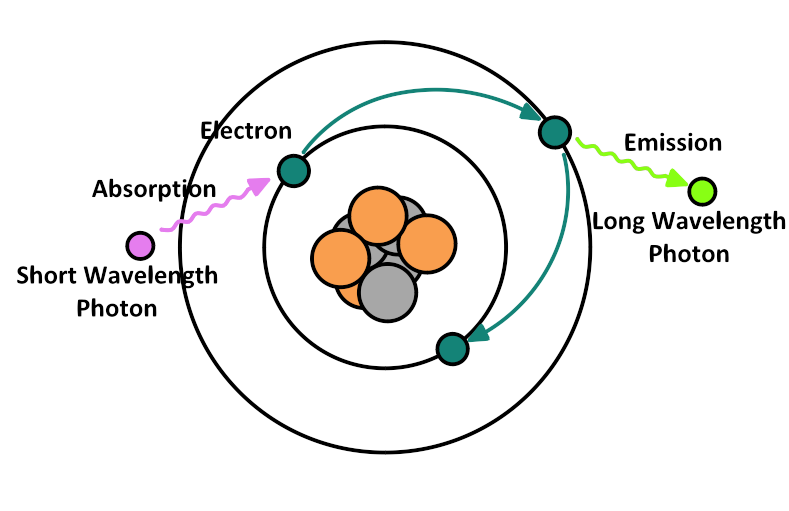
\includegraphics[width=0.4\columnwidth]{molecular_absorption.png}
		\label{fig:molecularabsorption}
	}
	\subfigure[]
	{
		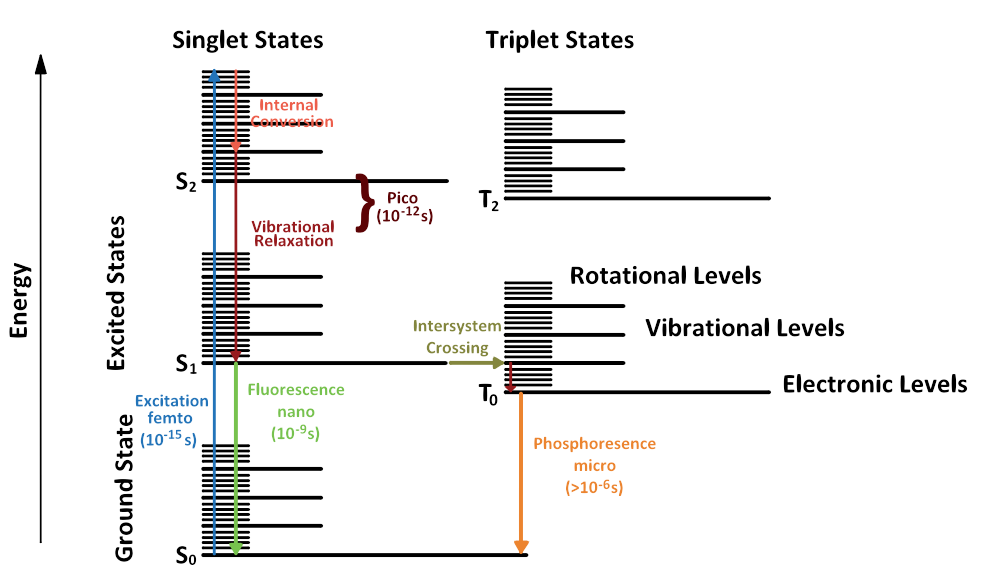
\includegraphics[width=0.56\columnwidth]{jablonski_diagram.png}
		\label{fig:jablonski}
	}
	\caption{\textbf{(a)} Simplified fluorescence process. \textbf{(b)} The Jab{\l}o{\'n}ski diagram depicting the electronics states from photon absorption to photo emission.}
	\label{fig:fluorescence_electron_states}
\end{figure}

The overall principle of fluorescence can be explained in three steps \citep{Nobel2016} as illustrated in \Cref{fig:molecularabsorption}: 
(1) Energy is absorbed by an atom upon collision with a photon.
(2) The atom becomes excited and an electron jumps to a higher energy level.
(3) Shortly after jumping to the higher energy level the electron returns to the ground state and emits a photon.

\begin{definition}[Excitation and emission]
	One of the best ways to visualise the fluorescing process is using a Jab{\l}o{\'n}ski diagram.
	A detailed Jab{\l}o{\'n}ski diagram is shown in \Cref{fig:jablonski}. 
	When a photon collides with an atom, all its energy is transferred to the atom. The energy of the photon is inversely related to it's wavelength, $E = h \frac{c}{\lambda}$, where $h$ is Planck's constant and $c$ and $\lambda$ are the speed and wavelength of light in a vacuum respectively.
	This increase in energy moves an electron from the ground state, $S_0$, to a higher energy level state.
	Depending on the energy of the photon and the number of photons absorbed by the electron, the electron can move to different energy levels e.g. $S_1, S_2, etc$.
	This process happens almost immediately in the order of femtoseconds($10^{-15}s$).
	Before moving to the next lowest energy level, $S_1$, some energy is lost due to internal conversion and vibrational relaxation.
	When the electron spontaneously decays from $S_1$ to $S_0$ it emits a photon of a longer wavelength than the absorption photon.
	This happens within a few nanoseconds ($10^{-9}s$) after excitation.
	
	The difference in wavelength of the emission photon and excitation photon is known as the \textit{Stokes' Shift} or \textit{Stokes' Law}.
	The larger the Stokes' Shift the easier it is to separate the emission light from the excitation light \citep{Spring2003}.
	The emission curve is often a mirror image and shifted to longer wavelengths than the excitation curve as illustrated in \Cref{fig:excitationandemissionspectra}.
\end{definition}

\begin{definition}[Fluorophores]
	Substances that exhibit the fluorescent property are called fluorophores, also known as \textit{fluorochromes} or \textit{fluoresent dyes}.
	Early investigations showed that many substance naturally posess fluorescent properties, such as minerals, crystals, resins, crude drugs, butter, chlorophyll, vitamins, etc \citep{Spring2003}.
	This is known as \textit{autofluorescence}.
	Substances that do not fluoresce must be \textit{stained} such that it can be observed through a fluorescent microscope.
	We will expand on this later in this chapter.
\end{definition}

%\begin{definition}[Jab{\l}o{\'n}ski diagrams]
%	Stuff for this section.
%\end{definition}

%\begin{definition}[Excitation spectra]
%	Stuff for this section. Electronic States
%\end{definition}

%\begin{definition}[Emission spectra]
%	Stuff for this section. Electronic States
%\end{definition}

\begin{definition}[Intersystem crossing]
	If the electron spin as the electron transfer between energy states is preserved then the energy states are known as \textit{singlet states}.
	It is also possible for the electron to reverse it's spin.
	However, this is very unlikely and is known as \textit{forbidden transition} in Quantum mechanics.
	When this happens the electron is said to be in a \textit{triplet state}, see \Cref{fig:jablonski}.
	The only way for the electron to reach the ground state is to undergo another forbidden transition, which is even less likely.
	When, eventually, this does happen, the electron may emit a photon; this phenomenon is known as \textit{phosphorescence}.
	This process takes much longer, in the order of microseconds ($10^{-6}s$).
\end{definition}

%\begin{definition}[Quantum yield]
%	Stuff for this section. Electronic States
%\end{definition}

\begin{figure}[!t]
	\centering
	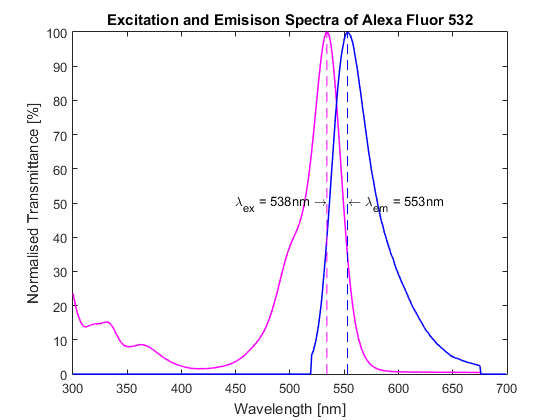
\includegraphics[width=\columnwidth]{alexafluor532_spectra.png}
	\caption{Normalised Excitation and Emmision Spectra of the Alexa Fluor 532 flurophore.
	The emmission maximum is at $553nm$ which is a more yellow-green than excitation maximum at $5534nm$.
	Data obtained from ThermoFisher Scientific \citep{AlexaFluor532}.}
	\addloflink{https://www.thermofisher.com/us/en/home/life-science/cell-analysis/labeling-chemistry/fluorescence-spectraviewer.html}
	\label{fig:excitationandemissionspectra}
\end{figure}

%----------------------------------------------------------------------------------------
%	SECTION 2
%----------------------------------------------------------------------------------------

\section{Specimen Labelling}
\label{sec:SpecimenLabelling}

%\textcolor{red}{Why do specimens have to be stained? What is is staining?}
Many of the components of interest, such as cell nuclei, cytoplasm, genes, chrosomes, proteins, do not possess a high degree of, if not any,  autofluorescence. 
In this scenario, these components can be marked with a fluorescent dye \citep{Tsien1998}, also known as a fluorophore or fluorochrome, a substance that can bind to a specific target whose excitation and emission spectra are well known. 
This is known as staining \citep{Danek2012,Hubeny2008,Dobrucki2013}. 
Once the specimen is stained it can be indirectly observed using a fluorescence microscope.

%\textcolor{red}{What are the most common staining protocols?}
The most prevalent staining techniques are fluorescence in-situ hybridisation (FISH) and immunostaining \citep{Danek2012,Fatima2008,Kozubek2001_2,Theodosiou2007}.

\begin{definition}[FISH staining]
	%\textcolor{red}{What is FISH?	What is the FISH staining techniques used for?}
	FISH is a molecular cytogenetic technique that uses flourophores that bind to selected regions in nucleic acids \citep{Danek2012,Fatima2008}.
	FISH is the most frequently used staining technique used primarily for visualisation and localisation of nucleic acid sequences, chromosomes, cytplasm or organelles which contain those acids \citep{Hubeny2008}.
	This makes FISH highly attractive for finding specific features in DNA and RNA used in genetic diagnosis and research, medicine and species identification \citep{Amann2008,Fatima2008}.
	Figure \ref{fig:FISH} is a microscope image of mouse chromosomes using the FISH staining technique.
\end{definition}

\begin{definition}[Immunostaining]
	%\textcolor{red}{What is Immunofluorescence and the two main types, what is the difference between the two, and which is more common? What is the Immunofluorescence staining techniques used for?}
	Immunofluorescence is the detection method where an antibody is used to detect an antigen in a tissue or a cell using fluorescence. Flourophores are usually conjugated onto antibodies, which are proteins that are designed bind to specific antigens, target proteins, on a cell \citep{CudeBurke2014}.
	The two types of immunofluorescent detection are immunocytofluorescence (ICF) and immunohystofluorescence (IHF).
	These must not be confused with immunocytochemistry (ICC) and immunohistochemistry (IHC).
	\textit{Immuno} refers to the immunological technique, i.e. the binding of antibodies to antigens.
	\textit{Cyto} refers to cells, i.e. cells without the extracellular membrane.
	\textit{Histo} refers to tissue i.e. cells with the extracellular membrane.
	\textit{Chemistry} refers to the chemical method of detection, e.g. a change in colour.
	\textit{Fluorescence} detection by emission of light \citep{Katikireddy2011}.
	Figure \ref{fig:IHC} shows the detection of the p53 Binding Protein 1 in perfusion fixed frozen sections of rat kidney.
\end{definition}

\begin{definition}[Live-cell staining]
	%\textcolor{red}{FISH and IHC cannot stain live cells. Why? How can we stain live cells?}
	The staining techniques discussed previously are not suitable to observe living cells.
	The fluorescent dyes that are used are phototoxic and cause cells to die. To circumvent this problem an elegant solution has been devised.
	Instead of staining, the cells are modified to produce a fluorescent substance in the target structures.
	Derivatives of the \textit{green fluorescent protein} (GFP), isolated from the \textit{Aequorea victoria} jellyfish \citep{Tsien1998,LichtmanConchello2005,Fatima2008}, are used as it generates a strong photon emission and is non-toxic to living cells \citep{Danek2012,Hubeny2008,Dobrucki2013}.
\end{definition}

%\textcolor{red}{Important notes about fluorophores and the impact on image quality?}

\begin{figure}[!t]
	\centering
	\subfigure[]
	{
		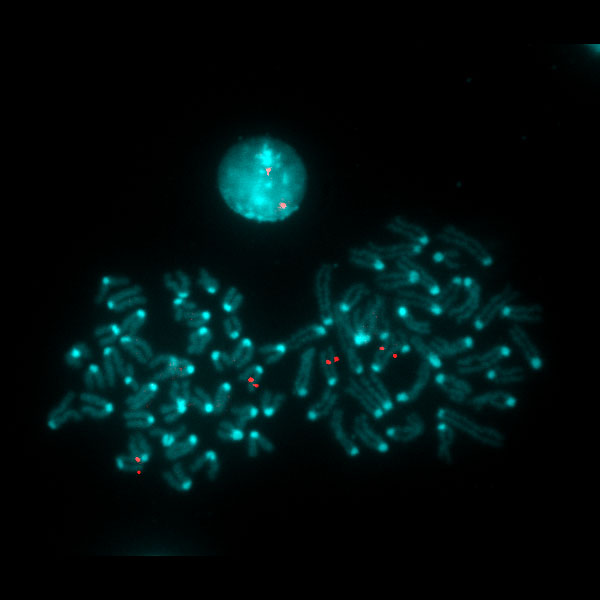
\includegraphics[width=0.495\columnwidth]{fish1.jpg}
		\label{fig:FISH}
	}
	\subfigure[]
	{
		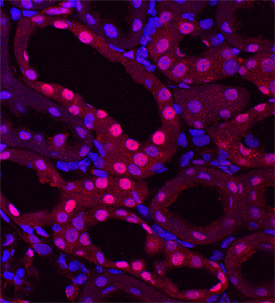
\includegraphics[width=0.45\columnwidth]{ihc1.jpg}
		\label{fig:IHC}
	}
	\caption{\textbf{(a)} FISH (Fluorescent 'in-situ' Hybridization) in mouse chromosomes using a BAC clone labeled with Spectrum Orange. The picture shows two metaphases and one interphase with two signals in each exampling a homozygous mouse for a transgenic clone. Image Source: "All About the Human Genome Project" Genetic and Genomic Image and Illustration Database. %\addloflink{https://unlockinglifescode.org/media/images/} %\url{https://unlockinglifescode.org/media/images/}. 
	\textbf{(b)} p53 Binding Protein 1 (53BP1) was detected in perfusion fixed frozen sections of rat kidney using Goat Anti-Human 53BP1 Antigen Affinity-purified Polyclonal Antibody (Catalog \# AF1877) at 15 $\mu$g/mL overnight at 4$^{\circ}$C. Tissue was stained using the NorthernLights\texttrademark 557-conjugated Anti-Goat IgG Secondary Antibody (red; Catalog \# NL001) and counterstained with DAPI (blue). Specific staining was localized to nuclei of epithelial cells in convoluted tubules. Image Source: R\&D Systems' IHC image database.}
	%\addloflink{https://www.rndsystems.com/resources/ihc-images/53bp1}}
	%\url{https://www.rndsystems.com/resources/ihc-images/53bp1}.}
	\addloflink{https://unlockinglifescode.org/media/images/}
	\addloflink{https://www.rndsystems.com/resources/ihc-images/53bp1}
	\label{fig:stainingtechniques}
\end{figure}

%----------------------------------------------------------------------------------------
%	SECTION 3
%----------------------------------------------------------------------------------------

\section{The Epifluorescence Microscope and Image Acquisition}
\label{sec:TheEpifluorescenceMicroscope}

\begin{figure}[!t]
	\centering
	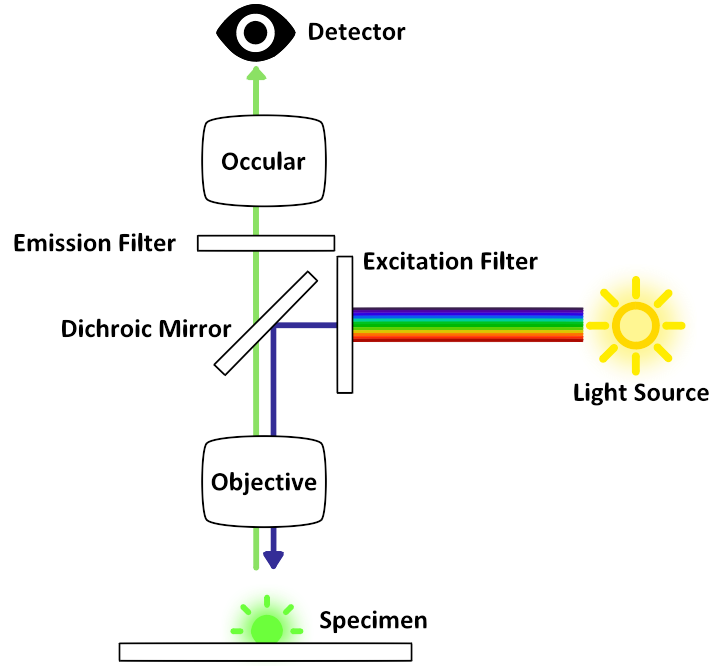
\includegraphics[width=0.4\columnwidth]{Epifluorescence_Microscope.png}
	\caption{The schematic of the epifluorescence microscope.}
	\label{fig:epifluorescencemicroscope}
\end{figure}

%\textcolor{red}{What is a fluorescent microscope? Schematic layout of a fluorescence microscope? Function and purpose of each component in the fluorescent microscope?}
A fluorescence microscope is an optical microscope that is designed specifically to exploit the principle of fluorescence to allow for the observation of flourescently labelled specimens \citep{Hubeny2008,Sarder2006,Dobrucki2013,Andrews2002,Fatima2008}.
There are many types of fluorescent micrcoscopes available but the preferred type among many biologists and geneticists is the epifluorescent microscope \citep{Rice2016,AbramowitzDavidson2016}.
A schematic of the epifluorescent micrcoscope is illustrated in \Cref{fig:epifluorescencemicroscope}.

\begin{definition}[Light source]
	%\textcolor{red}{What sort of light needs to be generated? What sort of lamps are used? Advantages and disadvantages of certain lamps.}
	The light source is typically a high-luminance light source e.g. Mercury or Xenon arc lamps, LEDs, lasers, etc  \citep{Danek2012,Hubeny2008,Aswani2012,Rice2016,ThermoFisher2016}.
	The primary criterion for choosing a light source is that its characeristic peaks must coincide with the excitation spectrum of the fluorophores being used \citep{LichtmanConchello2005,Spring2003,Fatima2008}.
	Wavelength coverage spans from near infra-red to UV.
	Mercury and Xenon arc lamps are expensive, an inexpensive and lightweight alternative are bright LEDs \citep{Fatima2008,Dobrucki2013,Aswani2012,Koch1972}.
\end{definition}

\begin{definition}[Excitation filter]
	%\textcolor{red}{What is an excitation filter? Why is it needed?}
	Typically, the incoming light from the light source is multispectral \citep{SpringDavisdson2016}. 
	The excitation filter is a wavelength selection filter which is placed in the path of the incoming light and filters through only those wavelengths in the absorption spectrum of the fluorescent dye \citep{ThermoFisher2016,Danek2012,Hubeny2008,LichtmanConchello2005,Spring2003,CudeBurke2014,Fatima2008,Dobrucki2013}.
\end{definition}

\begin{definition}[Dichroic mirror]
	%\textcolor{red}{What is a dichroic mirror? Why is it needed?}
	Also known as a \textit{dichroic beam splitter}.
	This is placed at a 45$^{\circ}$ angle and reflects the short-wavelenght light filtered through the excitation filter at a 90$^{\circ}$ angle towards the specimen \citep{Danek2012,Hubeny2008,Spring2003,CudeBurke2014} and allows the long-wavelength light from the fluorescing specimen to pass through to the detector \citep{LichtmanConchello2005,Koch1972}, thus serving as a separation filter between the absorption and emission light \citep{Fatima2008,Dobrucki2013}.
\end{definition}

\begin{definition}[Objective]
	%\textcolor{red}{What is the objective? Why is it needed?}
	The incoming light reflected of the dichroic mirror passes through the objective lens before reaching the specimen \citep{Danek2012,Hubeny2008,LichtmanConchello2005,Spring2003}.
	Emission light from the fluorescing specimen is gathered in the objective lens and passed through to the dichroic mirror.
\end{definition}

\begin{definition}[Specimen]
	%\textcolor{red}{Say something about the specimen, for wholeness sake.}
	The specimen is irradiated by the incoming light from the objective and emits long-wavelength light in all directions.
	The specimen is stained with a flourophore whose absorption and emission curves are well known.
	This is important since the light source and the interference filters are chosen using the peaks of these curves.
\end{definition}

\begin{definition}[Emission filter]
	%\textcolor{red}{What is an emission filter? Why is it needed?}
	Also known as a \textit{barrier filter} \citep{LichtmanConchello2005,Spring2003,Koch1972}.
	The light coming from the specimen contains multiple wavelengths and the dichroic mirror is used to filter out the shorter wavelength light.
	The emission filter is further  used to filter out the wavelengths that correspond to the emission wavelengths of the fluorophore \citep{CudeBurke2014,Danek2012,Hubeny2008,SpringDavisdson2016,ThermoFisher2016}.
\end{definition}

%\begin{definition}[Occular]
%	\textcolor{red}{What is the occular why is it needed?}
%	Purpose of the occular.
%\end{definition}

\begin{definition}[Detector]
	%\textcolor{red}{What is the detector why is it needed?}
	A detector is used to capture the emission light and can further digital form the image.
	The detector is usually a photodetector such as a charge-coupled device (CCD) camera or a photomultipler tube \citep{Danek2012,Hubeny2008,LichtmanConchello2005,Spring2003,Murphy2001}.
	It is vital that an appropriate detector is chosen as this has a direct impact on the image quality \citep{Fatima2008}.
\end{definition}

%\textcolor{red}{Other Types of Fluorescence Microscopes: Confocal, TIRF. Acquisition: CCD, Hardware setup effect on image quality, Numerical Aperture, Sub-diffraction}
The type of fluorescence image data that needs to be captured is application dependant and this impacts the decision on which type of microscope is to be used.
The \textit{widefield}, or conventional, microscope produces 2D image data.
3D image data cannot be captured directly.
Instead, a series of 2D images are captured to form a 2D stack. The 3D image is then constructed in software.
In this scenario, the most common choice of micrscope is the \textit{confocal laser scanning microscope} (CLSM).
This microscope system is expensive and acquisition is slower.
An economical alternative is the \textit{confocal spinning disk miscroscope}.
To detect single molecules, the preffered technique is \textit{total internal reflection fluorescence} (TIRF) which can be achieved by a modification of the epifluorescence micrcoscope.

%----------------------------------------------------------------------------------------
%	SECTION 4
%----------------------------------------------------------------------------------------

\section{Image Processing}
\label{sec:ImageProcessing}

%\textcolor{red}{Limitations in Fluorescence Imaging. Preprocessing: Point Spread Function deconvolution, etc. Segmentation }
Due to the physical nature of the fluorescence and image acquisition process, there are many factors that can degrade image quality.
There are measures that can be taken to largely mitigate some problems but they can never be completely eliminated.
The presence of these factors directly affect segmentation accuracy and subsequently higher level analysis.
Therefore, images are processed prior to segmentation to suppress the artefacts and reconstruct the original data \citep{Danek2012} or to enhance it.
\Cref{chap:Chapter7} takes a step in this vein.
Here we present some of the commonly occuring factors that reduce image quality and the methods used to mitigate them, and some of the techniques employed for segmentation.

\subsection{Preprocessing}
%\textcolor{red}{Write a little something on preprocessing.}

\begin{definition}[Nonuniform illumination]
	%\textcolor{red}{What causes uneven illumination? What techniques are done to reduce it's effect. Vignette effect, etc.}
	There are many factors that could contribute to nonuniform illumination.
	The specimen layer will not be uniformly lit if the  arc lamp is not properly focussed on the black aperture.
	To prevent this from happening a liquid light guide-based light source, which provides even illumination, may be used \citep{LichtmanConchello2005}.
	If the light brightness diminished towards the edges of the image then this is known as the \textit{Vignette effect}.
	Common techniques to suppress this distortion is \textit{background correction}, also known as \textit{flat-field correction}, \textit{background flattening} or \textit{shading correction} \citep{Danek2012,Fatima2008,Murphy2001}.
	Other causes of nonuniform illumination are inhomogenous detector sensitivity, autofluorescence, dirt particles in the optical system or nonspecific sample staining.
	An example of the Vignette effect is illustrated in \Cref{fig:Vignette}.
	Computational schemes to eliminate nonuniform illumination have been well researched, although recently it has not received too much attention \citep{Young2001,Ghauharali1998,Model2001,Model2001_2}.
	
	\begin{figure}[!t]
		\centering
		\subfigure[]
		{
			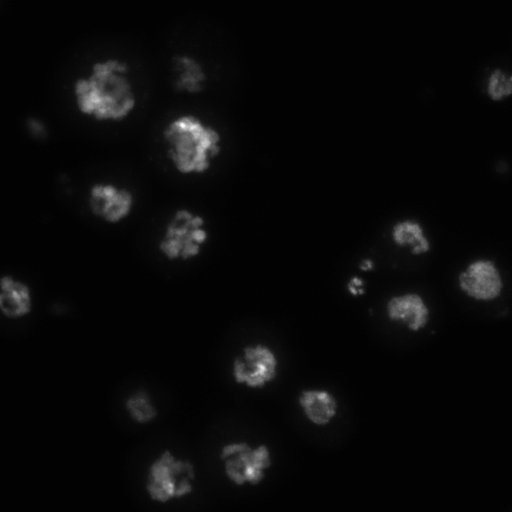
\includegraphics[width=0.31\columnwidth]{uneven_orig.jpg}
			\label{fig:ImageProcessingOriginal}
		}
		\subfigure[]
		{
			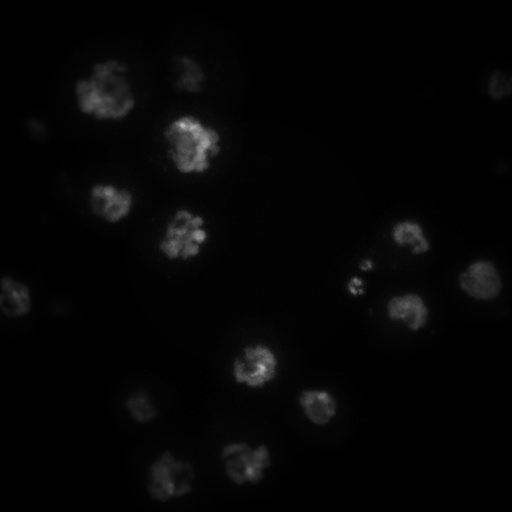
\includegraphics[width=0.31\columnwidth]{uneven.jpg}
			\label{fig:Vignette}
		}
		\subfigure[]
		{
			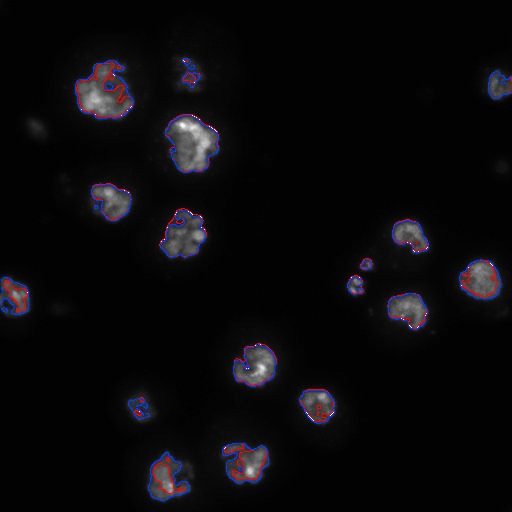
\includegraphics[width=0.31\columnwidth]{uneven_final.jpg}
			\label{fig:IlluminationSegmented}
		}
		\caption{The effect of nonuniform illumination on segmentation. \textbf{(a)} Original image. Image source: The Cell Image Library \citep{cil:21739}. \textbf{(b)} Nonuniformly illuminated image. The Vignette effect. \textbf{(c)} K-means clustering using the Euclidean distance metric and 2 clusters. The blue curve is from the original, the red curve is from the nonuniformly illuminated image. Notice that less of the object is recognised towards the edges.}
		\addloflink{http://www.cellimagelibrary.org/images/2173}
		\label{fig:illumination}
	\end{figure}
\end{definition}

\begin{definition}[Fading]
	%\textcolor{red}{What causes quenching and bleaching? What techniques are done to reduce it's effect. Why is photobleaching worse?}
	The reduction of emission intensity is called \textit{fading}, of which there are two types: \textit{quenching} and \textit{bleaching}.
	
	Quenching is a reversible loss of fluorescence owing to a variety of nonradiative energy-loss mechanisms such as collisions with nearby acceptor molecules, a phenomenon known as \textit{resonance energy transfer}.
	This phenomenon is useful in studying molelcular interactions below the lateral resolution of the light microscope through a technique called \textit{fluorescence resonance energy transfer} (FRET) \cite{Spring2003,Danek2012,LichtmanConchello2005}.
	
	Bleaching refers to all processes that cause a fluorescent signal to fade permanently \citep{LichtmanConchello2005}.
	From the fluorescence process presented in \Cref{sec:PhysicsOfFluorescence}, one may assume that, under the proper conditions, a fluorochrome has the ability to fluoresce indefinitely.
	However, this is not the case. There is a limited number of cycles before permanent bleaching \citep{LichtmanConchello2005}.
	\Cref{fig:bleaching} illustrates the effect of photobleaching.
	\textit{Photobleaching} is the most prominent form of bleaching.
	It is due the interaction of the fluorophore with an oxygen molecule.
	This can move the oxygen molecule to an excited singlet state, which then becomes a reactive molecule.
	When in this state, the oxygen molecule can participate in many chemically destructive reactions with organic molecules causing \textit{phototoxicity} \citep{Danek2012}.
	Photobleaching is used to study diffusion and motion through a technique called \textit{fluorescence recovery after photobleaching} (FRAP) \citep{LichtmanConchello2005,AbramowitzDavidson2016}.
	
	Photobleaching cannot be avoided but it be can pushed back.
	The aim in the measures to avoid photobleaching is to take a longer time to reach \textit{reciprocity failure} \citep{AbramowitzDavidson2016}.
	This is done by shortening exposure times and using less intensive excitation light.
	This, however, yields low contrast images.
	These images with low signal-to-noise \citep{Murphy2001} ratio (SNR) are more difficult to segment hence contrast enhancement must be performed on the images prior to segmentation \citep{Boppart2005}.
	\begin{figure}[!t]
		\centering
		\subfigure[]
		{
			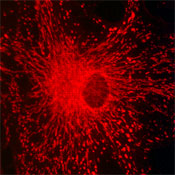
\includegraphics[width=0.31\columnwidth]{canvas.png}
			\label{fig:ImageProcessingOriginal2}
		}
		\subfigure[]
		{
			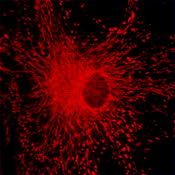
\includegraphics[width=0.31\columnwidth]{canvas10.png}
			\label{fig:Photobleach1}
		}
		\subfigure[]
		{
			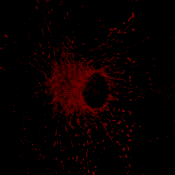
\includegraphics[width=0.31\columnwidth]{canvas20.png}
			\label{fig:Photobleach2}
		}
		\caption{The effect of photobleaching. Image Source: Molecular Expressions \citep{MolecularExpressionsPhotobleaching}. 
			\textbf{(a)} Original image at $t=0s$.
			\textbf{(b)} Image after $t=10s$.
			\textbf{(c)} Image after $t=20s$.
			}
		\label{fig:bleaching}
	\end{figure}
\end{definition}

\begin{definition}[Image distortion]
	%\textcolor{red}{What causes image distortion (PSF)? What techniques are done to reduce it's effect.}
	The major contributing factors to image distortion are: The \textit{point spread function} (PSF) and noise \citep{Sarder2006}.
	Image formation can be approximated by 
	\begin{equation}
		O = n(s \otimes h),
	\end{equation}
	where $O$ is the formed image, $n$ is the noise function, $s$ is the exact image and $h$ is the specific PSF of the optical system.
	We discuss the PSF first.
	The observed image is not an exact representation of the real object.
	Optical systems have an inherent property called 'the point spread function' which is the systems optical response to a point light source \citep{Danek2012}.
	The final image is dependant on the spatial position of a point, numerical aperture (NA) and furthermore differs for various emission wavelengths \citep{Hubeny2008,Keuper2012}.
	The final image is a superposition of all points in the illuminated volume where the contribution of each is described by the PSF.
	
	Theoretically the exact image can be obtained by deconvolution of the observed image with the PSF.
	However, there are secondary factors that prevent this.
	Deconvolution seeks to reconstruct the original image given the PSF and certain assumptions about noise \citep{Keuper2012}.
	This is an \textit{ill-posed problem} as little is known about the specific PSF or the noise model.
	Additionally, if the image is corrupted by too much of noise, deconvolution might still produce unsatisfactory results.
	The PSF is generally experimentally determined or theorectically modelled, and so the true PSF is never attained.
	Hence, the original image can never be attained by deconvolving with an approximated PSF.
	The image formation and restroration process is illustrated in \Cref{fig:imageformation}.
	
	\begin{figure}[!t]
		\centering
		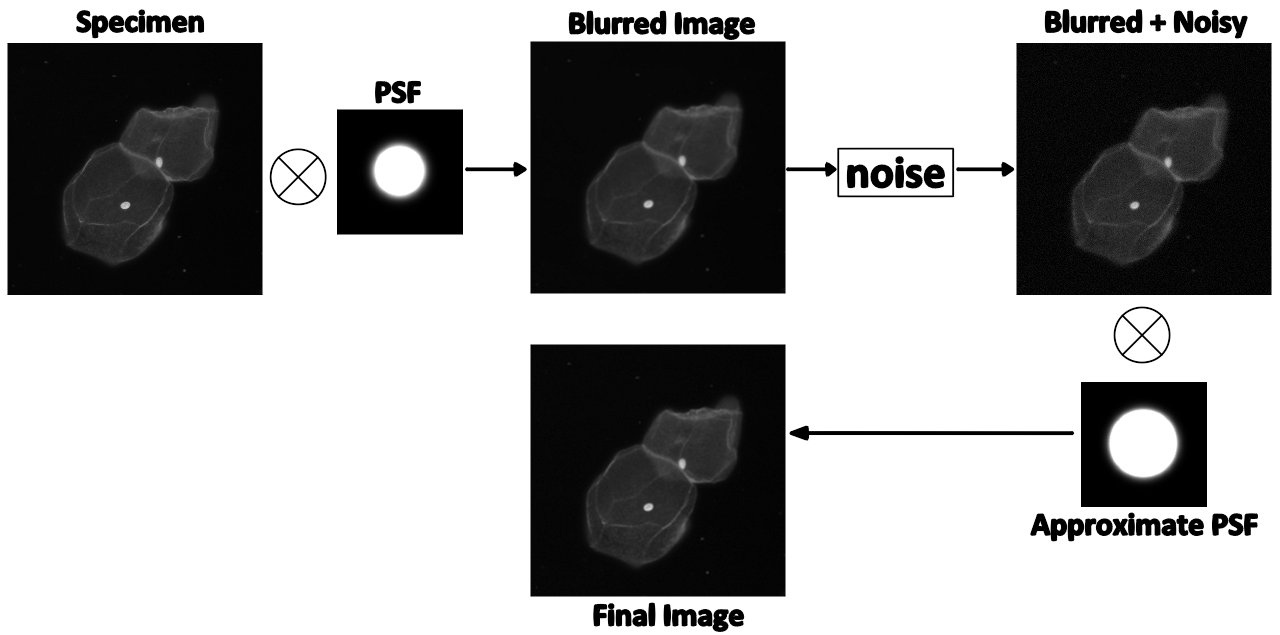
\includegraphics[width=\columnwidth]{image_formation.png}
		\caption{The image formation process. Image source: \citep{cil:40968}}
		\label{fig:imageformation}
	\end{figure}
	
	%Image deconvolution is a well researched and still an ongoing research topic.
	Deconvolution has recieved a lot of attention in the past with very creative approaches \citep{Mukamel2012,Verveer2007,Periasamy1999,Swedlow2007,Rooi2014}.
	Fluorescence microscopy deconvolution is still a very active field of research.
	Bayesian methods have become popular in fluorescence microscopy image deconvolution, however noise in low SNR imaging conditions still poses a challenge \citep{Wong2015}.
	Recent trends in 3D deconvolution in widefield microscopy use blind depth-invariant of the PSF \citep{Kim2015}.
	Most PSF deconvolution systems na{\"i}vely assume depth-invariance however, the PSF changes significantly along the optical axis.
	There are also deconvolution methods that can preserve detail and possibly enhance image quality in diffraction-limited/superresolution imaging modalilities \citep{Qin2016}.
\end{definition}

\begin{definition}[Noise]
%\textcolor{red}{What types of noise are most prevalent? How do they arise? What techniques are done to reduce it's effect.}
As previously stated, fluorescence imaging is a low light, low constrast and low SNR imaging technique to counter the effects of bleaching.
For these reasons, noise becomes prominent. The three types of noise recorded by a camera is \textit{dark noise}, \textit{read noise} and \textit{photon noise} \citep{Dobrucki2013,Danek2012,Matula2012,Hubeny2008}.

The electrons in a CCD of film are always in motion due to thermal energy.
Dark current is due to the extraneous electrons which are excited into the signal.
This signal carries a statistical fluctuation known as dark noise.
Dark current effects can be reduced by ground image subtraction or cooling the CCD.
If there is a significant amount of dark noise then the background will not be as black as is necessary.
For this reason it is common to mistake dark noise for low-level autofluorescence \citep{Ryan2016,Dobrucki2013}.

Read noise is a result of the conversion process from charge build-up to a voltage and then digitisation.

Photon noise, also known as \textit{shot noise}, is the signal dependant statical variation of the counting of photons incident on the CCD or film.
This is a naturally occuring phenomenon and cannot be reduced by camera design of system optimisation \cite{Ryan2016}.

In low-light imaging techniques, such as is common in fluorescence imaging, the dominant form of noise is photon noise.
Photon noise and dark noise are Poisson distributed \citep{Danek2012,Ryan2016,Kempen1999}.
Noise is low-light images used to modelled using the Gaussian distribution but was found to be a poor description of the noise.
The Poisson distribution provides a more physically accurate model especially in photon-limited recording \citep{Sarder2006}.
We study deonising in \Cref{sec:PoissonDenoising}.
The effect of noise on segementation accuracy is illustrated in \Cref{fig:Noise}.

\begin{figure}[!t]
	\centering
	\subfigure[]
	{
		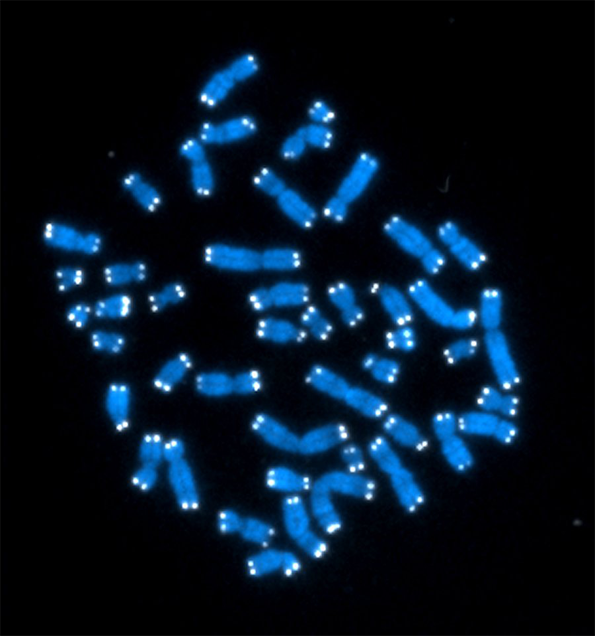
\includegraphics[width=0.31\columnwidth]{poisson2.png}
		\label{fig:ImageProcessingOriginal3}
	}
	\subfigure[]
	{
		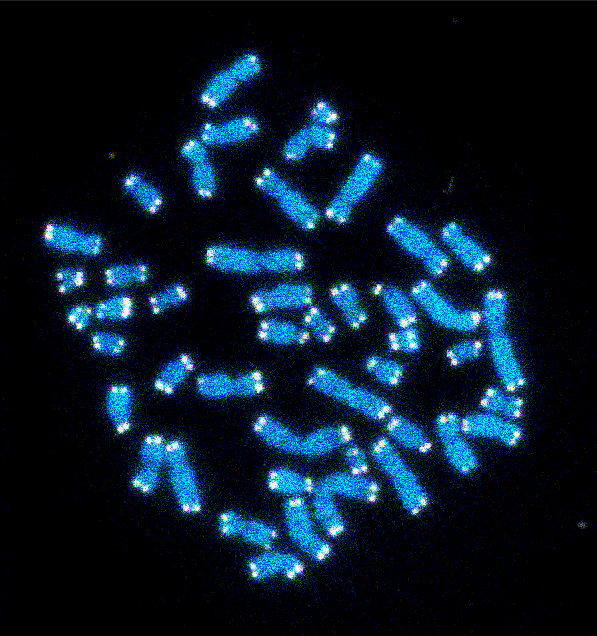
\includegraphics[width=0.31\columnwidth]{poisson.png}
		\label{fig:PoissonNoise}
	}
	\subfigure[]
	{
		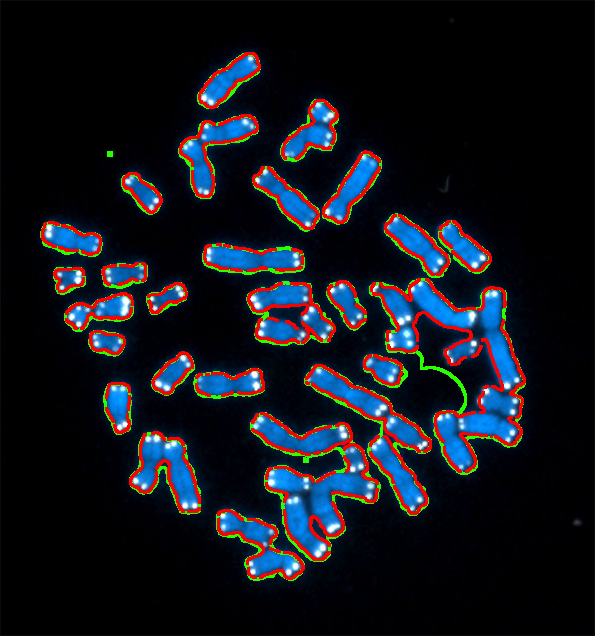
\includegraphics[width=0.31\columnwidth]{poisson_final.png}
		\label{fig:NoiseSegmented}
	}
	\caption{The effect of noise on segmentation. 
		\textbf{(a)} Original image. 
		\textbf{(b)} Poisson noise corrupted image.
		\textbf{(c)} ACWE Chan-Vese segmentated output. The red curve is from the original, the green curve is from the Poisson noise corrupted image. Notice that there are more artifacts and the segmented output is less accurate especially towards the bottom left from the green curve.}
	\label{fig:Noise}
\end{figure}
\end{definition}

\subsection{Segmentation}
%\textcolor{red}{Write a little something on segmentation in cell imaging. Basic historical track of cell segmentation. Focus on specfic segmentation techniques.}
The primary aim of using fluorescence microscopy imaging is to make diagnoses and to study molecular behaviour and interaction.
This means that biologists, geneticists and other professionals alike, not only have a superabundance of microscopic imaging techniques at their disposal, but also have an immense amount of image data to analyse since the outburst of image acquisition technology.
The abundance, diversity, dimensionality and complexity of fluorescence image data obviates manual image processing as this isn't tractable, by any means, in terms of time or quality \citep{Meijering2012,Ryan2016}.
Consequently, the task has fallen to computers to perform these tasks and has now become essential in advancing these fields \citep{Alberts2007,Vonesch2006}.
The crux of image analysis lies on the accuracy of image segmentation and has become the principle focus in many studies \citep{Bengtsson2004}.\\

Anton van Leeuwenhoek, a Dutch draper and scientist, is credited with the invention of the first real compound microscope in the late 17th century.
However, it wasn't until the mid-1950s that computers became involved when systems were developed to automate the classification of smears of exfoliated cells.
These systems used simple thresholding rules on 1D scanning of microscopic lines \citep{Tolles1955}.
In the 1960s, automated systems were developed to count leukocytes on 2D image data based on their colour and morphological measurements \citep{Prewitt1966}.
In the 1980s the invention of the confocal microscope made it possible to study cells in 3D but it wasn't until the 1990s that the computer became powerful enough to process 3D image data or complex 2D images \citep{Gurcan2009}.
The trends of increased computing power has made possible the use of more sophisticated cell analysis techniques as well as the ability to use more computationally demanding segmentation methods.
The literature on cell segmentation and analysis has experienced exponential growth in the last couple of decades.
Many studies comparing segmentation algorithms for cells have been pubished \citep{Dima2011,Pincus2007,Coelho2009}.
We review some of the common techniques used in fluorescence microscopy image segmentation.

\begin{definition}[Intensity thresholding]
	%\textcolor{red}{Say something about this section.}
	Intensity thresholding assumes a non-overlapping intensity levels between the objects and the background.
	It is still one of the most common thresholding methods for cell segmentation \citep{WuMerchantCastleman2008,Meijering2004,Quanli2011}.
	Locally adaptive thresholding techniques are used when illumination varies across the image.
	Automated threshold segmentation techniques are usually based on global or local intensity using the histogram \citep{Bengtsson2004}.
	Thresholding produces suboptimal results due to the na{\"i}ve assumption of mutually exclusive intensity levels.
\end{definition}

\begin{definition}[Morphological segmentation]
	%\textcolor{red}{Say something about this section.}
	This method uses non-linear mathematical morphological operators like erosion, dilation, opening, closing, etc with geometrical and topological properties to segment the image \citep{GonzalezWoods2002,Meijering2004,Dorini2007,Anoraganingrum1999,Kumar2002}.
	Generally, this method is used as a post-processing step to refine a coarse segmentation; or as a pre-processing step to suppress certain image structures \citep{Bengtsson2004}.
\end{definition}

\begin{definition}[Region accumulation]
	%\textcolor{red}{Say something about this section.}
	This method starts with selected points, called seeds.
	The idea is to iteratively add points neighboring previously labelled pixels based on some conformity measure, usually intensity.
	The most common implementation is called \textit{region growing}.
	Most cases assume an image model similar to that of thresholding and suffers the same segmented results problems.
	Another approach is called the \textit{watershed method} which converts the image into an open 3D shape and "fills the shape with water".
	The different regions are separated by those "filled with water" and those that aren't.
	A common problem with this method is oversegmentation and usually requires post-processing methods, like \textit{region merging}, to achieve a meaningful result \citep{Jiang2003,Lin2003,Bengtsson2004}.
\end{definition}

\begin{definition}[Edge-based segmentation]
	%\textcolor{red}{Say something about this section.}
	There are basically two types of edge-based segmentation: \textit{gradient based methods} and \textit{Laplacian based methods}.
	
	Gradient methods are based on the assumption that there is a rapid intensity gradient between the object and the background.
	Edges are detected by searching for the maximum and minimum in the first derivative, e.g. Prewitt, Roberts and Sobel operators.
	
	Laplacian methods search for zero-crossings in the second derivative, e.g. Marr-Hildreth, Laplacian of Gaussian (LoG), Canny edge detection.
	
	These algorithms are very fast to compute but the drawback is when closed curves are desired \citep{Bengtsson2004}, which is a common criterion in biological and molecular segmentation.
	A solution to this is to use snakes or active shape models.
\end{definition}

\begin{definition}[Energy minimisation]
	%\textcolor{red}{Two types: Deformable models and Graph cuts}
	The most recent segmentation methods are based on energy minimisation.
	Most current state-of-the-art techniques fall under this category.
	This is due to their flexibility and robustness \citep{Danek2012}.
	This group encompasses two main subgroups: \textit{deformable models} and \textit{discrete combinatorial optimisation}.
	
	The aim of deformable model techniques is to fit a deformable model, either a curve or a surface, to the image data.
	They may be formulated either explicitely, as a parametric contour (2D) or a surface, e.g. snakes \citep{Kass1988} or active contours \citep{Caselles1997,Li2009,Cheng2009}, or implicitely as a zero-level of a function with one dimension higher than that of the image data, e.g. as a level set \citep{Osher2003}.
	This technique widely used in fluorescence image segmentation \citep{Dzyubachyk2008,Ortiz2001,Dufour2005,Dzyubachyk2010,Boukari2014,Maska2007}.
	
	The aim discrete combinatorial optimisation is to search a finite countable solution space for the optimal solution.
	Optimality is defined with respect to some energy function, which embeds one or more criteria, which is to be minimised.
	The most common implementation exploits the graph cut framework.
	Graph cut segmentation has recently gained a lot of popularity and momentum in medical image segmentation (MIS) \citep{Danek2009,Chen2008,Kofahi2010,Kong2011,Yang2009,Zhang2014,Liu2008,Vu2008}.
\end{definition}

\begin{definition}[Other miscellaneous techniques]
	%\textcolor{red}{Unsupervised clustering (k-means), Otsu binarization , dynamic programming , Voronoi diagrams , ellipse fitting, template matching, model matching, gradient flow tracking.}
	The techniques presented are just a select few in a plethora segmentation techniques that have been used in microscopy image segmentation.
	A few other common techniques are unsupervised clustering segmentation using the k-means \citep{Ng2006,Shrivastava2014,Dhanachandra2015}, Otsu binarization \citep{Chen2006}, dynamic programming \citep{Liu2007,Zhang2007}, Voronoi diagrams \citep{Cardenes2003,Jiang2005}, gradient flow tracking \citep{Li2007}, etc.
	This is just a few more.
	Instead of cell segmentation converging to a robust, flexible and unified solution, the number of available options is steadily increasing \citep{Meijering2012}.
	There probably exists as many individual unique solutions for cell segmentation as there are problems.
\end{definition}

%----------------------------------------------------------------------------------------
%	SECTION 5
%----------------------------------------------------------------------------------------

\section{Object Measurement and Analysis}
\label{sec:Measurements}

%\textcolor{red}{What is the purpose of object analysis in FM? What is measured?}
The aim in fluorescence image analysis is to measure specific properties of interest which enable higher level decision making.
Typically, these properties are quantitative measures.
In this section we review some of the important quantitative measurements in digital image analysis.
It is important to note that for some of the properties of interest, the accuracy of the measurements depend heavily on the accuracy on the segmentation.
The properties of interest are application dependent, one might require solely the object morphology of structure and hence properties like perimeter, area, shape, intensity, colour, etc, are of significance.
Alternatively, if one requires the colocalisation of cells, then distance discriminants, such as Euclidean distance, Manhattan distance, Chessboard distance, etc, are of significance \citep{Fatima2008_2,Danek2012}.

Object measures can be loosely classified into four catergories: geometric measures, histogram-based measures, intensity based measures and temporal measures. One can also argue a fifth catergory statistical classifiers although this is generally used in higher level analysis.

\begin{definition}[Size measures]
	Perimeter, area and volume are common measures to describe the size of objects.
	Area and volume are suitable measures to describe the general size of an object.
	The perimeter of an object is distinctly useful in discriminating its shape complexity. Complex and irregular shapes need a larger perimeter to enclose its area.
\end{definition}

\begin{definition}[Pose measures]
	This measure is defines an objects location and orientation.
	The centroid is used as an objects' locale and its orientation is the measure of the angle subtended by its major axis.
\end{definition}

\begin{definition}[Shape measures]
	Shape features are used to distinguish objects from one another.
	These measures are generally translationally, rotationally and scale invariant and can be used independent of, or in conjunction with, the size measures.
	Commonly assessed shape parameters are thinness ratio to describe the regularity of an object, rectangularity, circularity, Euler number, moments, central moments, object dispersion, rotationally invariant moments, Zernike moments and elongation.
\end{definition}

\begin{definition}[Shape descriptors]
	Shapes descriptors provide a more wholesome way of decribing an object's shape than compared to the single parameter shape measures.
	Differential chain codes, and its two most common descriptors boundary chain code (BCC) and differential chain code (DCC), are used to represent the distance around an object.
	Fourier descriptors is another object distance measure that expliots the periodicity of BCC.
	There are also graph respresentations of which the two most common are minimum spanning tree (MST) \citep{Giesen2014,Yuan2009} and Delaunay triagulation (DT) \citep{Kozubek2000,Attali1997}.
\end{definition}

\begin{definition}[Distance measures]
	There are many ways to compute the separation between objects.
	The most commonly assessed distance measures are Euclidean distance, Manhattan distance (also known as the City-block distance or absolute value metric), which is a more computationally efficient approximation of Euclidean distance, and the Chessboard distance (also known as the maximum value metric) \citep{French2008,Zinchuk2007}.
\end{definition}

\begin{definition}[Intensity measures]
	Images are segmented generally into region with low intra-region intensity distribution and high inter-region intensity distribution \citep{Pinkel1986,Meijering2004}.
	Common intensity measures are integrated optical density (IOD) \citep{Loferer1998,Watanabe1991}, is simply the sum of all the gray levels that compose the object, its a reflection of  the object's "mass" or "weight", average optical density (AOD), is the IOD divided by the objects area, and contrast.
\end{definition}

\begin{definition}[Histogram measures]
	These measure provide a measure of an object's intensity distribution.
	Common histogram-based measures are mean, standard deviation, skew, entropy and energy \citep{Rust2006,Boland2001}.
\end{definition}

\begin{definition}[Texture measures]
	In image analysis texture refers to the spatial arrangement of gray level values \citep{Duda2001} and hence a texture feature quantifies some characteristic of the intensity variation within an object.
	Common texture measures are statistical texture measures, gray-level co-occurrence matrix (GLCM) \citep{Atlamazoglou2001,Cicchi2010} and power spectrum features \citep{Erik1999,Xu1996}.
\end{definition}

\begin{definition}[Ratiometric measures]
	Some fluorescent dye respond to the changes in Calcium and Hydrogen ion concentration by changing its spectral properties of the fluorescent emission bands. In this case, a ratio of the intensity can be used to calculate concentration of calcium of pH value \citep{Dobrucki2013}.
\end{definition}

\begin{definition}[Temporal measures]
	Considering the time domain, many interesting properties can be observed.
	Commonly computed properties of interest are motility \citep{Sekar2003,Miller1869,Mathur2000}, like velocity and acceleration, rate of growth, rate of change of colour, etc.
\end{definition}

These measures are used in higher decision making processes such as the evaluation of a hypothesis to detect the presence of a certain disease. They are also used to aid in the understanding of biological mechanisms, events and interatctions \citep{Danek2012}. % Fluorescence Microscopy
%% Chapter Template

\chapter{Mathematical Background} % Main chapter title

\label{chap:Chapter2} % Change X to a consecutive number; for referencing this chapter elsewhere, use \ref{ChapterX}

%----------------------------------------------------------------------------------------
%	SECTION 1
%----------------------------------------------------------------------------------------

\section{Graph Theory and Flow Networks}
\label{sec:GraphTheory}

In this section we cover Graph Theory and specifically Flow Networks, which is a branch of Graph Theory, which is fundamental to the understanding of image segmentation via graph cuts. With it roots in Germany where Euler tried to find the solution to the Konigsberg bridge problem, graph theory has since blossomed into a rich field of Mathematics with seemingly endless amounts of application. Graph Theory is a huge topic in mathematics and can be applied to many other sciences. Graph theory is part of another more encompassing field of Mathematics known as Combinatronics. Graph theory and applications are more useful than the average person would recognise. They're used in Google Maps to find shortest routes to destinations, in Molecular Chemistry to model the structure of atoms, and the list goes on for quite a while. It is no surprise that it is also found to be useful in image segmentation.

\begin{definition}[Graph]\label{def_graph}
	A graph $G$ is a pair $(V,E)$, where $V$ is the set of nodes/vertices and $E$ is the set of edges consisting of pairs $(u,v)$ where $u,v \in V$. The graph is assumed to be finite i.e. $|V| = n$ and $|E| = m$.
\end{definition}

In an \textbf{undirected graph}, the edge $(u,v)$ and $(v,u)$ are not distinct. That is, they refer to the same edge. However, in a \textbf{directed graph}, the two edge are now distinct. In a directed graph with edge $(u,v)$, $u$ is known as the \textbf{tail} and $v$ is know as the \textbf{head}. In directed graphs, edges, also known as arcs, are depicted by placing arrowheads at the head of the edge. Given an edge $e = (u,v)$, $u$ and $v$ are said to be \textbf{incident} on $e$. A graph is said to be \textbf{simple} if it does not contain any self-loops. A \textbf{self-loop} is an edge with of its end points being the same vertex.

\begin{definition}[Degree]
	The degree of a vertex $v$ is the number of edges incident on it. $deg(v) = |\{(u,v), (v,u) \in E\}|$. A self-loop counts for 2.
\end{definition}

If a graph is directed, also known as a \textbf{digraph}, then a node $v$ has an \textbf{in-degree} $d_{in}(v)$ and an \textbf{out-degree} $d_{out}(v)$. A digraph is said to be \textbf{balanced} if $d_{in}(v) = d_{out}(v), \forall v \in V$.

\tikzstyle{vertex}=[circle,thick,draw]
\tikzstyle{edge} = [draw=black!24, very thick,-]
\tikzstyle{weight} = [font=\small]
\begin{figure}[!h]
	\centering
	\resizebox {\columnwidth} {!} {
		\begin{tikzpicture}[scale=1.5, auto, swap, background rectangle/.style={fill=blue!10}, show background rectangle]
		\draw[black] node at (-0.2,2.8) [font=\large,right,rounded corners,inner sep=1ex] {$\textbf{G}$};
		% draw the vertices
		\foreach \pos/\name in {{(0,2)/a}, {(2,2)/b}, {(4,1)/c},{(0,0)/d}, {(3,0)/e}, 
			{(4,-1)/g}, {(1,-1)/f}}
		\node[vertex] (\name) at \pos {$\name$};
		% connect vertices with edges and draw weights
		\foreach \source/ \dest /\weight in {b/a/10,c/b/3,d/a/5,d/b/7, e/b/9, e/c/7,e/d/5,
			f/d/3,f/e/1, g/e/3,g/f/5}
		\path[edge] (\source) -- node[weight] {$\weight$} (\dest);
		% info box
		\draw[yshift=0cm,xshift=4.5cm]
		node [right,text width=5cm,rounded corners,fill=red!20,inner sep=1ex]
		{
			$V_{G} = \{a,b,c,d,e,f,g\}$, \\
			$|V_{G}| = 7$\\
			$E_{G} = \{ab,ad,bc,bd,be,ce,de,df,ef,$\\$eg,fg\}$, \\ 
			$|E_{G}| = 11$
		};	
		% degrees
		\draw[orange] node at (-0.2,2.4) [font=\footnotesize,right,rounded corners,inner sep=1ex] {$d(a)=2$};
		\draw[orange] node at (1.8,2.4) [font=\footnotesize,right,rounded corners,inner sep=1ex] {$d(b)=3$};
		\draw[orange] node at (3.8,1.4) [font=\footnotesize,right,rounded corners,inner sep=1ex] {$d(c)=2$};
		\draw[orange] node at (-0.3,-0.5) [font=\footnotesize,right,rounded corners,inner sep=1ex] {$d(d)=4$};
		\draw[orange] node at (3.2,0.0) [font=\footnotesize,right,rounded corners,inner sep=1ex] {$d(e)=5$};
		\draw[orange] node at (0.8,-1.5) [font=\footnotesize,right,rounded corners,inner sep=1ex] {$d(f)=3$};
		\draw[orange] node at (3.8,-1.5) [font=\footnotesize,right,rounded corners,inner sep=1ex] {$d(g)=2$};
		\end{tikzpicture}
	}
	\caption{Undirected weighted graph \textbf{G}. The degree of each node is shown next to the corresponding node. The graph is simple. The red box shows the vertex set, $V_{G}$, and edge set, $E_{G}$, and their corresponding norm.}
\end{figure}

\tikzstyle{vertex}=[circle,thick,draw]
\tikzstyle{edge} = [draw=black!24, very thick,<-]
\tikzstyle{weight} = [font=\small]
\begin{figure}[!h]
	\centering
	\resizebox {\columnwidth} {!} {
		\begin{tikzpicture}[scale=1.5, auto, swap, background rectangle/.style={fill=blue!10}, show background rectangle, >={Stealth[black!24]}]
		\draw[black] node at (-0.2,3.1) [font=\large,right,rounded corners,inner sep=1ex] {$\textbf{D}$};
		% draw the vertices
		\foreach \pos/\name in {{(0,2)/a}, {(2,2)/b}, {(4,1)/c},{(0,0)/d}, {(3,0)/e}, 
			{(4,-1)/g}, {(1,-1)/f}}
		\node[vertex] (\name) at \pos {$\name$};
		% connect vertices with edges and draw weights
		\foreach \source/ \dest /\weight in {b/a/10,c/b/3,d/a/5,e/b/9,e/d/5,
			f/d/3,f/e/1, g/e/3,g/f/5}
		\path[edge] (\source) edge node[weight] {$\weight$} (\dest);
		% bend edges
		\path [edge] (b) edge[bend right=20] node {$7$} (d);
		\path [edge] (d) edge[bend left=-20] node {$4$} (b);
		\path [edge] (e) edge[bend right=20] node {$7$} (c); 
		\path [edge] (c) edge[bend right=20] node {$2$} (e);
		% info box
		\draw[yshift=0cm,xshift=4.5cm]
		node [right,text width=5cm,rounded corners,fill=red!20,inner sep=1ex]
		{
			$V_{D} = \{a,b,c,d,e,f,g\}$, \\
			$|V_{D}| = 7$\\
			$E_{D} = \{ab,ad,bc,bd,be,ce,db,de,df,$\\$ec,ef,eg,fg\}$, \\
			$|E_{D}| = 13$
		};
		% degrees
		% a	
		\draw[orange] node at (-0.2,2.7) [font=\footnotesize,right,rounded corners,inner sep=1ex] {$d_{in}=0$};
		\draw[orange] node at (-0.2,2.4) [font=\footnotesize,right,rounded corners,inner sep=1ex] {$d_{out}=2$};	
		% b
		\draw[orange] node at (1.8,2.7) [font=\footnotesize,right,rounded corners,inner sep=1ex] {$d_{in}=2$};
		\draw[orange] node at (1.8,2.4) [font=\footnotesize,right,rounded corners,inner sep=1ex] {$d_{out}=5$};
		% c
		\draw[orange] node at (3.8,1.7) [font=\footnotesize,right,rounded corners,inner sep=1ex] {$d_{in}=2$};
		\draw[orange] node at (3.8,1.4) [font=\footnotesize,right,rounded corners,inner sep=1ex] {$d_{out}=1$};
		% d
		\draw[orange] node at (-0.3,-0.5) [font=\footnotesize,right,rounded corners,inner sep=1ex] {$d_{in}=2$};
		\draw[orange] node at (-0.3,-0.8) [font=\footnotesize,right,rounded corners,inner sep=1ex] {$d_{out}=2$};
		% e
		\draw[orange] node at (3.2,0.08) [font=\footnotesize,right,rounded corners,inner sep=1ex] {$d_{in}=3$};
		\draw[orange] node at (3.2,-0.12) [font=\footnotesize,right,rounded corners,inner sep=1ex] {$d_{out}=3$};
		% f
		\draw[orange] node at (0.8,-1.5) [font=\footnotesize,right,rounded corners,inner sep=1ex] {$d_{in}=2$};
		\draw[orange] node at (0.8,-1.8) [font=\footnotesize,right,rounded corners,inner sep=1ex] {$d_{out}=1$};
		%g
		\draw[orange] node at (3.8,-1.5) [font=\footnotesize,right,rounded corners,inner sep=1ex] {$d_{in}=2$};
		\draw[orange] node at (3.8,-1.8) [font=\footnotesize,right,rounded corners,inner sep=1ex] {$d_{out}=0$};
		\end{tikzpicture}
	}
	\caption{Directed weighted graph (Digraph) \textbf{D}. The in-degree and out-degree is shown next to each node. The graph is simple and not balanced. The red box shows the vertex set, $V_{D}$, and edge set, $E_{D}$, and their corresponding norm.}
\end{figure}

\begin{definition}[Subgraph]
	A graph $G' = (V', E')$ is said to be a sub-graph of $G = (V, E)$, denoted as $G' \subseteq G$, if $V' \subseteq V$ and $E' \subseteq E$.
\end{definition}

\tikzstyle{vertex}=[circle,thick,draw]
\tikzstyle{edge} = [draw=black!24, very thick,-]
\tikzstyle{weight} = [font=\small]
\begin{figure}[!h]
	\centering
	\resizebox {\columnwidth} {!} {
		\begin{tikzpicture}[scale=1.5, auto, swap, background rectangle/.style={fill=blue!10}, show background rectangle]
		\draw[black] node at (-0.2,2.8) [font=\large,right,rounded corners,inner sep=1ex] {$\textbf{H}$};
		% draw the vertices
		\foreach \pos/\name in {{(0,2)/a}, {(2,2)/b}, {(0,0)/d}, {(3,0)/e}}
		\node[vertex] (\name) at \pos {$\name$};
		% connect vertices with edges and draw weights
		\foreach \source/ \dest /\weight in {b/a/10,d/a/5,d/b/7,e/b/9,e/d/5}
		\path[edge] (\source) -- node[weight] {$\weight$} (\dest);
		% info box
		\draw[yshift=-1.6cm,xshift=0cm]
		node [right,text width=5cm,rounded corners,fill=red!20,inner sep=1ex]
		{
			$V_{H} = \{a,b,d,e\} \subseteq V_{G}$, \\
			$|V_{H}| = 4$\\
			$E_{H} = \{ab,ad,bd,be,de\} \subseteq E_{G}$, \\ 
			$|E_{H}| = 5$
		};	
		% degrees
		\draw[orange] node at (-0.2,2.4) [font=\footnotesize,right,rounded corners,inner sep=1ex] {$d(a)=2$};
		\draw[orange] node at (1.8,2.4) [font=\footnotesize,right,rounded corners,inner sep=1ex] {$d(b)=3$};
		\draw[orange] node at (-0.2,-0.4) [font=\footnotesize,right,rounded corners,inner sep=1ex] {$d(d)=4$};
		\draw[orange] node at (2.5,-0.4) [font=\footnotesize,right,rounded corners,inner sep=1ex] {$d(e)=5$};
		
		
		\draw[black] node at (4.2,2.8) [font=\large,right,rounded corners,inner sep=1ex] {$\textbf{I}$};
		% draw the vertices
		\foreach \pos/\name in {{(4.4,2)/a}, {(6.4,2)/b}, {(4.4,0)/d}, {(7.4,0)/e}}
		\node[vertex] (\name) at \pos {$\name$};
		% connect vertices with edges and draw weights
		\foreach \source/ \dest /\weight in {b/a/10,d/a/5,e/b/9,e/d/5}
		\path[draw=black!24, very thick,<-] (\source) -- node[weight] {$\weight$} (\dest);
		% bends
		\path [draw=black!24, very thick,<-] (d) edge[bend left=-20] node {$4$} (b);
		% info box
		\draw[yshift=-1.6cm,xshift=4.4cm]
		node [right,text width=5cm,rounded corners,fill=red!20,inner sep=1ex]
		{
			$V_{I} = \{a,b,d,e\} \subseteq V_{D}$, \\
			$|V_{I}| = 4$\\
			$E_{I} = \{ab,ad,bd,be,de\} \subseteq E_{D}$, \\ 
			$|E_{I}| = 5$
		};	
		% degrees
		% a	
		\draw[orange] node at (4.2,2.5) [font=\footnotesize,right,rounded corners,inner sep=1ex] {$d_{in}=0$};
		\draw[orange] node at (4.2,2.3) [font=\footnotesize,right,rounded corners,inner sep=1ex] {$d_{out}=2$};	
		% b
		\draw[orange] node at (6.2,2.5) [font=\footnotesize,right,rounded corners,inner sep=1ex] {$d_{in}=1$};
		\draw[orange] node at (6.2,2.3) [font=\footnotesize,right,rounded corners,inner sep=1ex] {$d_{out}=2$};
		% d
		\draw[orange] node at (4.1,-0.4) [font=\footnotesize,right,rounded corners,inner sep=1ex] {$d_{in}=2$};
		\draw[orange] node at (4.1,-0.6) [font=\footnotesize,right,rounded corners,inner sep=1ex] {$d_{out}=1$};
		% e
		\draw[orange] node at (7.1,-0.4) [font=\footnotesize,right,rounded corners,inner sep=1ex] {$d_{in}=2$};
		\draw[orange] node at (7.1,-0.6) [font=\footnotesize,right,rounded corners,inner sep=1ex] {$d_{out}=0$};
		\end{tikzpicture}
	}
	\caption{Undirected weighted graph \textbf{H} is a subgraph of \textbf{G} in Figure XX, $\textbf{H} \subseteq \textbf{G}$. Directed weighted graph \textbf{I} is a subgraph of \textbf{D} in Figure XX, $\textbf{I} \subseteq \textbf{D}$. The degree of each node is shown next to the corresponding node. The red box shows the vertex set, the edge set and their corresponding norms.}
\end{figure}


\begin{definition}[Clique]
	A clique is a maximal subgraph.
\end{definition}

\begin{definition}[Network]
	A network $N = (V,E)$ is a directed graph with a source node $s$, a sink node $t$ and a strictly positive capacity on every edge. That is, for each edge $e \in E$, the capacity, $c(.)$, obeys $c(e) \in \Re^{+}$.
\end{definition}

\tikzstyle{vertex}=[circle,thick,draw]
\tikzstyle{edge} = [draw=black!24, very thick,->]
\tikzstyle{weight} = [font=\small]
\begin{figure}[!h]
	\centering
	\resizebox {\columnwidth} {!} {
		\begin{tikzpicture}[scale=1.5, auto, swap, background rectangle/.style={fill=blue!10}, show background rectangle, >={Stealth[black!24]}]
		\draw[black] node at (-0.2,1.5) [font=\large,right,rounded corners,inner sep=1ex] {$\textbf{N}$};
		
		\draw node[circle,thick,right,fill=red!20,text=red!20] at (-0.2,0) {$s$};
		\draw node[circle,thick,right,fill=red!20,text=red!20] at (5.8,0) {$t$};
		\draw[dashed,draw=red!24,very thick] (0.0,0) -- (0.5,-1.5);
		\draw[dashed,draw=red!24,very thick] (6.0,0) -- (6.5,-1.5);
		\draw[dashed,draw=red!24,very thick] (2.65,1.25) -- (4,1.5);
		
		% draw the vertices
		\foreach \pos/\name in {{(0,0)/s},{(2,1)/a},{(4,1)/b},{(2,-1)/c},{(4,-1)/d}, {(6,0)/t}}
		\node[vertex] (\name) at \pos {$\name$};
		% connect vertices with edges and draw weights
		\foreach \source/ \dest /\weight in {s/a/7,s/c/2,a/b/{},c/d/2,b/t/5,d/t/3}
		\path[edge] (\source) edge node[weight] {$\weight$} (\dest);
		% bends
		\path [draw=black!24, very thick,->] (a) edge[bend left=-30] node {$3$} (d);
		\path [draw=black!24, very thick,->] (c) edge[bend left=30] node {$3$} (b);
		% info box		
		\draw node[circle,right,fill=red!20] at (2.65,1.25) {$5$};
		\draw node[right,rounded corners,fill=red!20,inner sep=1ex] at (4,1.5){$capacity$};
		\draw node[right,rounded corners,fill=red!20,inner sep=1ex] at (0,-1.5){$source$};
		\draw node[right,rounded corners,fill=red!20,inner sep=1ex] at (6,-1.5){$sink$};
		% s	
		\draw[orange] node at (-0.2,0.4) [font=\footnotesize,right,rounded corners,inner sep=1ex] {$d_{in}=0$};
		\draw[orange] node at (-0.2,0.7) [font=\footnotesize,right,rounded corners,inner sep=1ex] {$d_{out}=2$};	
		% t
		\draw[orange] node at (5.8,0.4) [font=\footnotesize,right,rounded corners,inner sep=1ex] {$d_{in}=2$};
		\draw[orange] node at (5.8,0.7) [font=\footnotesize,right,rounded corners,inner sep=1ex] {$d_{out}=0$};
		\end{tikzpicture}
	}
	\caption{Network \textbf{N} with no flow. The in-degree and out-degree for the source, \textbf{s}, and the sink, \textbf{t}, are shown next to the corresponding node.}
\end{figure}

The \textbf{source node} only has out-going edges, $d_{in}(s) = 0$ and $d_{out}(s) \geq 0$. The \textbf{sink node} only has incoming edges, $d_{in} \geq 0$ and $d_out = 0$.

\begin{definition}[Flow]
	A flow $f : V^2 \longrightarrow \Re^{+}$ is associated with each edge $e = (u,v)$ such that:
	\begin{enumerate}
		\item for each edge $e \in E$ we have $0 \leq f(e) \leq c(e)$. That is, the flow is positive and cannot excees the capacity of the edge.
		
		\item for each intermediate node $v \in V\setminus \{s,t\}$ the in- and out-flow of that node $\sum_{u \in V^-(v)} f(u,v) = \sum_{u \in V^+(v)} f(v,u)$.
	\end{enumerate}
\end{definition}

The \textbf{total flow} $F$ of a network is then what leave the source $s$ or reaches the sink $t$:
\begin{equation}
F(N) := \sum_{u \in V} f(s,u) - \sum_{u \in V}f(u,s) = \sum_{u \in V} f(u,t) - \sum_{u \in V}f(t,u)
\end{equation}

\tikzstyle{vertex}=[circle,thick,draw]
\tikzstyle{edge} = [draw=black!24, very thick,->]
\tikzstyle{weight} = [font=\small]
\begin{figure}[!h]
	\centering
	\resizebox {\columnwidth} {!} {
		\begin{tikzpicture}[scale=1.5, auto, swap, background rectangle/.style={fill=blue!10}, show background rectangle, >={Stealth[black!24]}]
		\draw[black] node at (-0.2,1.5) [font=\large,right,rounded corners,inner sep=1ex] {$\textbf{N}$};
		\draw node[circle,thick,right,fill=red!20,text=red!20] at (-0.2,0) {$s$};
		\draw node[circle,thick,right,fill=red!20,text=red!20] at (5.8,0) {$t$};
		\draw[dashed,draw=red!24,very thick] (2.65,1.25) -- (4,1.5);
		\draw[dashed,draw=red!24,very thick] (0.0,0) -- (0.5,-1.5);
		\draw[dashed,draw=red!24,very thick] (6.0,0) -- (6.5,-1.5);
		% draw the vertices
		\foreach \pos/\name in {{(0,0)/s},{(2,1)/a},{(4,1)/b},{(2,-1)/c},{(4,-1)/d}, {(6,0)/t}}
		\node[vertex] (\name) at \pos {$\name$};
		% connect vertices with edges and draw weights
		\foreach \source/ \dest /\weight in {s/a/{5/7},s/c/{2/2},a/b/{},c/d/{1/2},b/t/{4/5},d/t/{3/3}}
		\path[edge] (\source) edge node[weight] {$\weight$} (\dest);
		% bends
		\path [draw=black!24, very thick,->] (a) edge[bend left=-30] node {$1/3$} (d);
		\path [draw=black!24, very thick,->] (c) edge[bend left=30] node {$2/3$} (b);
		% info box		
		\draw node[rounded corners,right,fill=red!20] at (2.65,1.25) {$3/5$};
		\draw node[right,rounded corners,fill=red!20,inner sep=1ex] at (4,1.5){$flow/capacity$};
		% s	
		\draw node[right,rounded corners,fill=red!20,inner sep=1ex] at (0,-1.5) [font=\footnotesize,right,rounded corners,inner sep=1ex] {$\sum\limits_{u \in V_N} f(s,u)=7$};
		% t
		\draw node[right,rounded corners,fill=red!20,inner sep=1ex] at (6,-1.5) [font=\footnotesize,right,rounded corners,inner sep=1ex] {$\sum\limits_{u \in V_N} f(u,t)=7$};
		\end{tikzpicture}
	}
	\caption{Network \textbf{N} with flow. The flow out of the source node, \textbf{s}, is equal to the flow into the sink node, \textbf{t}. For all other nodes, the flow-in is equal to the flow-out. This is the conservation of flow principle. This is only part of the network. The remaining part is the residual graph which shows the amount of reverse flow is available on an edge.}
\end{figure}

\begin{definition}[Cut]
	A cut of a network $N = (V,E)$ is a partitioning of the vertex set $V = P \bigcup \bar{P}$ into two disjoint sets $P$ containining the source node $s$ and $\bar{P}$ containing the sink node $t$. $P \bigcap \bar{P} = \emptyset$.
\end{definition}

\tikzstyle{vertex}=[circle,thick,draw]
\tikzstyle{edge} = [draw=black!24, very thick,->]
\tikzstyle{weight} = [font=\small]
\begin{figure}[!h]
	\centering
	\resizebox {\columnwidth} {!} {
		\begin{tikzpicture}[scale=1.5, auto, swap, background rectangle/.style={fill=blue!10}, show background rectangle, >={Stealth[black!24]}]
		\draw[black] node at (-0.2,1.5) [font=\large,right,rounded corners,inner sep=1ex] {$\textbf{N}$};
		\path[fill=red!20,,use Hobby shortcut,closed=true] (-0.3,-0.1) .. (1,1) .. (2.3,1.2) .. (1.3,0.2);
		%		\draw node[text=blue] at (-0.3,0) {$1$};
		%		\draw node[text=blue] at (1,1) {$2$};
		%		\draw node[text=blue] at (2.5,1.2) {$3$};
		%		\draw node[text=blue] at (1,0.0) {$4$};
		\path[fill=blue!20,,use Hobby shortcut,closed=true] (1.5,-1) .. (2.5,0.5) .. (3.5,1.2) .. (5.2,1.0) .. (6.3,0.0) .. (5.0,-1);
		%		\draw node[text=blue] at (1,-1) {$1$};
		%		\draw node[text=blue] at (3.2,1.2) {$2$};
		%		\draw node[text=blue] at (5.0,1.2) {$3$};
		%		\draw node[text=blue] at (6.5,0.0) {$4$};
		% draw the vertices
		\foreach \pos/\name in {{(0,0)/s},{(2,1)/a},{(4,1)/b},{(2,-1)/c},{(4,-1)/d}, {(6,0)/t}}
		\node[vertex] (\name) at \pos {$\name$};
		% connect vertices with edges and draw weights
		\foreach \source/ \dest /\weight in {s/a/{},s/c/{},a/b/{},c/d/{},b/t/{},d/t/{}}
		{
			\path[edge] (\source) edge node[weight] {$\weight$} (\dest);
		}		
		% bends
		\path [draw=black!24,very thick,->,name path=curve1] (a) edge[bend left=-30] node {} (d);
		\path [draw=black!24,very thick,->,name path=curve2] (c) edge[bend left=30] node {} (b);
		% cut
		\draw node [text=orange] at (0,-0.7) {$C$};
		\path[dashed, very thick, draw=orange, name path=C] (0,-1) -- (3.5,1.5);
		% intersections
		\path [draw=black!24,name path=line1] (s) -- (c);		
		\path [draw=black!24,name path=line2] (a) -- (b);		
		\path [draw=blue!24,name path=line3] (a) edge [bend left=-30] (d);
		\fill [color=orange, name intersections={of=C and line1}] (intersection-1) circle (2pt);
		\fill [color=orange, name intersections={of=C and line2}] (intersection-1) circle (2pt);
		\fill [color=orange, name intersections={of=C and line3}] (2.15,0.53) circle (2pt);	
		% info box
		\draw[yshift=-2.1cm,xshift=-0.5cm]
		node [right,rounded corners,fill=orange!20,inner sep=1ex]
		{
			$S = \{s,a\}$, \, $T = \{t,b,c,d\}$, \,$C = \{(sc), (ab), (ad)\}$
		};
		\end{tikzpicture}
	}
	\caption{Network \textbf{N} with with a valid cut \textbf{C}. The nodes within the red region are reachable from the source and the nodes within the blue region are able to reach the sink. The cut set, \textbf{C}, is show in the orange filled block.}
\end{figure}

\tikzstyle{vertex}=[circle,thick,draw]
\tikzstyle{edge} = [draw=black!24, very thick,->]
\tikzstyle{weight} = [font=\small]
\begin{figure}[!h]
	\centering
	\resizebox {\columnwidth} {!} {
		\begin{tikzpicture}[scale=1.5, auto, swap, background rectangle/.style={fill=blue!10}, show background rectangle, >={Stealth[black!24]}]
		\draw[black] node at (-0.2,1.5) [font=\large,right,rounded corners,inner sep=1ex] {$\textbf{N}$};
		\path[fill=red!20,,use Hobby shortcut,closed=true] (-0.3,-0.1) .. (2,1.5) .. (4,1.5) .. (6.4,-0.1) .. (4,0) .. (2,0) ;
		%				\draw node[text=blue] at (-0.3,0) {$1$};
		%				\draw node[text=blue] at (2,1.5) {$2$};
		%				\draw node[text=blue] at (4,1.5) {$3$};
		%				\draw node[text=blue] at (6.3,0.0) {$4$};
		%				\draw node[text=blue] at (4,0.0) {$5$};
		%				\draw node[text=blue] at (2,0.0) {$6$};
		\path[fill=blue!20,,use Hobby shortcut,closed=true] (1.5,-1) .. (3.0,-0.7) .. (4.5,-1.0) .. (3.0,-1.2);
		%				\draw node[text=blue] at (1.5,-1) {$1$};
		%				\draw node[text=blue] at (3.0,-0.7) {$2$};
		%				\draw node[text=blue] at (4.5,-1.0) {$3$};
		%				\draw node[text=blue] at (3.0,-1.2) {$4$};			
		% draw the vertices
		\foreach \pos/\name in {{(0,0)/s},{(2,1)/a},{(4,1)/b},{(2,-1)/c},{(4,-1)/d}, {(6,0)/t}}
		\node[vertex] (\name) at \pos {$\name$};
		% connect vertices with edges and draw weights
		\foreach \source/ \dest /\weight in {s/a/{},s/c/{},a/b/{},c/d/{},b/t/{},d/t/{}}
		{
			\path[edge] (\source) edge node[weight] {$\weight$} (\dest);
		}		
		% bends
		\path [draw=black!24,very thick,->,name path=curve1] (a) edge[bend left=-30] node {} (d);
		\path [draw=black!24,very thick,->,name path=curve2] (c) edge[bend left=30] node {} (b);
		% cut
		\draw node [text=orange] at (0,-0.7) {$C$};
		\path[dashed, very thick, draw=orange, name path=C] (0,-1) edge[bend left=30] (6,-1);
		% intersections
		\fill [color=orange] (1.0,-0.5) circle (2pt);
		\fill [color=orange] (5.0,-0.5) circle (2pt);
		\fill [color=orange] (2.28,-0.18) circle (2pt);
		\fill [color=orange] (2.52,-0.165) circle (2pt);
		% info box
		%		\draw[yshift=-2.1cm,xshift=-0.5cm]
		%		node [right,rounded corners,fill=orange!20,inner sep=1ex]
		%		{
		%			$S = \{s,a\}$, \, $T = \{t,b,c,d\}$, \,$C = \{(sc), (ab), (ad)\}$
		%		};
		\end{tikzpicture}
	}
	\caption{Network \textbf{N} with with a invalid cut \textbf{C}. The cut does not partition source node \textbf{s} and sink node \textbf{t} into distinct sets.}
\end{figure}

\tikzstyle{vertex}=[circle,thick,draw]
\tikzstyle{edge} = [draw=black!24, very thick,->]
\tikzstyle{weight} = [font=\small]
\begin{figure}[!h]
	\centering
	\resizebox {\columnwidth} {!} {
		\begin{tikzpicture}[scale=1.5, auto, swap, background rectangle/.style={fill=blue!10}, show background rectangle, >={Stealth[black!24]}]
		\draw[black] node at (-0.2,1.5) [font=\large,right,rounded corners,inner sep=1ex] {$\textbf{N}$};
		%		\path[fill=red!20,,use Hobby shortcut,closed=true] (-0.3,-0.1) .. (2,1.5) .. (4,1.5) .. (6.4,-0.1) .. (4,0) .. (2,0) ;
		%				\draw node[text=blue] at (-0.3,0) {$1$};
		%				\draw node[text=blue] at (2,1.5) {$2$};
		%				\draw node[text=blue] at (4,1.5) {$3$};
		%				\draw node[text=blue] at (6.3,0.0) {$4$};
		%				\draw node[text=blue] at (4,0.0) {$5$};
		%				\draw node[text=blue] at (2,0.0) {$6$};
		%		\path[fill=blue!20,,use Hobby shortcut,closed=true] (1.5,-1) .. (3.0,-0.7) .. (4.5,-1.0) .. (3.0,-1.2);
		%				\draw node[text=blue] at (1.5,-1) {$1$};
		%				\draw node[text=blue] at (3.0,-0.7) {$2$};
		%				\draw node[text=blue] at (4.5,-1.0) {$3$};
		%				\draw node[text=blue] at (3.0,-1.2) {$4$};			
		% draw the vertices
		\foreach \pos/\name in {{(0,0)/s},{(2,1)/a},{(4,1)/b},{(2,-1)/c},{(4,-1)/d}, {(6,0)/t}}
		\node[vertex] (\name) at \pos {$\name$};
		% connect vertices with edges and draw weights
		\foreach \source/ \dest /\weight in {s/a/{},s/c/{},a/b/{},c/d/{},b/t/{},d/t/{}}
		{
			\path[edge] (\source) edge node[weight] {$\weight$} (\dest);
		}		
		% bends
		\path [draw=black!24,very thick,->,name path=curve1] (a) edge[bend left=-30] node {} (d);
		\path [draw=black!24,very thick,->,name path=curve2] (c) edge[bend left=30] node {} (b);
		% cut
		\draw node [text=orange] at (0,-0.7) {$C$};
		\draw [dashed, orange, very thick] plot [smooth] coordinates {(0,-1) (2.5,1) (3,1.2) (3.5,-1.5)};
		% intersections
		\fill [color=orange] (0.77,-0.37) circle (2pt);
		\fill [color=orange] (2.09,0.68) circle (2pt);
		\fill [color=orange] (2.5,1) circle (2pt);
		\fill [color=orange] (3.05,1) circle (2pt);
		\fill [color=orange] (3.12,0.7) circle (2pt);
		\fill [color=orange] (3.40,-0.82) circle (2pt);
		\fill [color=orange] (3.42,-1) circle (2pt);
		% info box
		%		\draw[yshift=-2.1cm,xshift=-0.5cm]
		%		node [right,rounded corners,fill=orange!20,inner sep=1ex]
		%		{
		%			$S = \{s,a\}$, \, $T = \{t,b,c,d\}$, \,$C = \{(sc), (ab), (ad)\}$
		%		};
		\end{tikzpicture}
	}
	\caption{Network \textbf{N} with with a invalid cut \textbf{C}. The cut partition partitions the graph into more than two sets and the cut intersects the edges $ab$ and $ad$ twice.}
\end{figure}

The \textbf{capacity} of a cut is the sum of the edges $(u,v) \in V$ where $u \in P$ and $v \in \bar{P}$:
\begin{equation}
\kappa (P, \bar{P}) = \sum_{u \in P; v \in \bar{P}} c(u,v)
\end{equation}

\begin{definition}[Maximal Flow]
	The largest amount of flow that can be sent through the source that is able to reach the sink is known as the maximal flow.
\end{definition}

\tikzstyle{vertex}=[circle,thick,draw]
\tikzstyle{edge} = [draw=black!24, very thick,->]
\tikzstyle{weight} = [font=\small]
\begin{figure}[!h]
	\centering
	\resizebox {\columnwidth} {!} {
		\begin{tikzpicture}[scale=1.5, auto, swap, background rectangle/.style={fill=blue!10}, show background rectangle, >={Stealth[black!24]}]
		\draw[black] node at (-0.2,1.5) [font=\large,right,rounded corners,inner sep=1ex] {$\textbf{N}$};
		\draw node[circle,thick,right,fill=red!20,text=red!20] at (-0.2,0) {$s$};
		\draw node[circle,thick,right,fill=red!20,text=red!20] at (5.8,0) {$t$};
		\draw[dashed,draw=red!24,very thick] (0.0,0) -- (0.5,-1.5);
		\draw[dashed,draw=red!24,very thick] (6.0,0) -- (6.5,-1.5);
		% draw the vertices
		\foreach \pos/\name in {{(0,0)/s},{(2,1)/a},{(4,1)/b},{(2,-1)/c},{(4,-1)/d}, {(6,0)/t}}
		\node[vertex] (\name) at \pos {$\name$};
		% connect vertices with edges and draw weights
		\foreach \source/ \dest /\weight in {s/a/{6/7},s/c/{2/2},a/b/{5/5},c/d/{2/2},b/t/{5/5},d/t/{3/3}}
		\path[edge] (\source) edge node[weight] {$\weight$} (\dest);
		% bends
		\path [draw=black!24, very thick,->] (a) edge[bend left=-30] node {$0/3$} (d);
		\path [draw=black!24, very thick,->] (c) edge[bend left=30] node {$1/3$} (b);
		%info
		% s	
		\draw node[right,rounded corners,fill=red!20,inner sep=1ex] at (0,-1.5) [font=\footnotesize,right,rounded corners,inner sep=1ex] {$\sum\limits_{u \in V_N} f(s,u)=8$};
		% t
		\draw node[right,rounded corners,fill=red!20,inner sep=1ex] at (6,-1.5) [font=\footnotesize,right,rounded corners,inner sep=1ex] {$\sum\limits_{u \in V_N} f(u,t)=8$};
		\end{tikzpicture}
	}
	\caption{Network \textbf{N} with maximum flow. There is no way to push more flow out of the source into the sink without breaking the rules for conservation of flow.}
\end{figure}

\begin{definition}[Minimal Cut]
	A cut $C$ on a network $N = (V,E)$ is a minimal cut if there exists no other cut $C'$ where $\kappa (C') < \kappa(C)$.
\end{definition}

\tikzstyle{vertex}=[circle,thick,draw]
\tikzstyle{edge} = [draw=black!24,very thick,->]
\tikzstyle{weight} = [font=\small]
\begin{figure}[!h]
	\centering
	\resizebox {\columnwidth} {!} {
		\begin{tikzpicture}[scale=1.5, auto, swap, background rectangle/.style={fill=blue!10}, show background rectangle, >={Stealth[black!24]}]
		\draw[black] node at (-0.2,1.5) [font=\large,right,rounded corners,inner sep=1ex] {$\textbf{N}$};	
		\path[fill=red!20,,use Hobby shortcut,closed=true] (-0.3,-0.1) .. (2,1.5) .. (4,1.5) .. (4.5,-0.1) .. (4,-1.5) .. (2,-1.5) ;
		%			\draw node[text=blue] at (-0.3,0) {$1$};
		%			\draw node[text=blue] at (2,1.5) {$2$};
		%			\draw node[text=blue] at (4,1.5) {$3$};
		%			\draw node[text=blue] at (6.3,0.0) {$4$};
		%			\draw node[text=blue] at (4,-1.5) {$5$};
		%			\draw node[text=blue] at (2,-1.5) {$6$};
		\path[fill=blue!20,use Hobby shortcut,closed=true] (5.5,0) .. (6.0,0.5) .. (6.5,0) .. (6.0,-0.5);
		%			\draw node[text=blue] at (5.5,0) {$1$};
		%			\draw node[text=blue] at (6.0,0.5) {$2$};
		%			\draw node[text=blue] at (6.5,0) {$3$};
		%			\draw node[text=blue] at (6.0,-0.5) {$4$};
		% draw the vertices
		\foreach \pos/\name in {{(0,0)/s},{(2,1)/a},{(4,1)/b},{(2,-1)/c},{(4,-1)/d}, {(6,0)/t}}
		\node[vertex] (\name) at \pos {$\name$};
		% connect vertices with edges and draw weights
		\foreach \source/ \dest /\weight in {s/a/7,s/c/2,a/b/{5},c/d/2,b/t/5,d/t/3}
		\path[edge] (\source) edge node[weight] {$\weight$} (\dest);
		% bends
		\path [draw=black!24, very thick,->] (a) edge[bend left=-30] node {$3$} (d);
		\path [draw=black!24, very thick,->] (c) edge[bend left=30] node {$3$} (b);
		% cut
		\draw node [text=orange] at (4.8,-1.0) {$C$};
		\path[dashed, very thick, draw=orange, name path=C] (5,-1.2) -- (5,1.2);
		% intersections
		\path [draw=black!24,name path=line1] (b) -- (t);
		\path [draw=black!24,name path=line2] (d) -- (t);
		\fill [color=orange, name intersections={of=C and line1}] (intersection-1) circle (2pt);
		\fill [color=orange, name intersections={of=C and line2}] (intersection-1) circle (2pt);
		%info
		% minimum capacity	
		\draw node[right,rounded corners,fill=orange!20,inner sep=1ex] at (5,-1.5) [font=\footnotesize,right,rounded corners,inner sep=1ex] {$\sum\limits_{e \in C} c(e)=8$};
		\end{tikzpicture}
	}
	\caption{Network \textbf{N} with minimal cut \textbf{C}. The sum of the capacity of all the edges in the cut set is the minimum of all possible valid cuts on the network \textbf{N}.}
\end{figure}

In the next section we show that the Maximal Flow problem and the Minimal Cut problem are duals of each other, commonly known as the Max-Flow/Min-Cut problem.

%----------------------------------------------------------------------------------------
%	SECTION 2
%----------------------------------------------------------------------------------------

\section{Markov Random Fields}
\label{sec:MarkovRandomFields}

In this section we review MRF's as a pure mathematical/statistical tool used used specifically for vision. That is, we only cover the necessary concepts related to understanding 
the problem of modelling images for analysis and inference purposes. In sub-section 1 we cover the basics, in sub-section 2 we cover how to model an image using MRF, and 
in sub-section 3 we cover how to find the MAP, or a close enough approximation, to the MRF.

%-----------------------------------
%	SUBSECTION 1
%-----------------------------------

\subsection{Markov Random Fields Theory and Concepts}

MRF theory and concepts. Purely mathematical/statistical.
Markov Properties\\
Markov Blankets

%-----------------------------------
%	SUBSECTION 2
%-----------------------------------

\subsection{Markov Random Fields in Image Modelling}

Modelling the joint probability of of image using MRFs.
Nearby pixels exhibit high correlation in natural images. This is where we can take advantage of Markov Modelling.

%-----------------------------------
%	SUBSECTION 3
%-----------------------------------

\subsection{MAP-MRF Approxiamtion via Graph Cuts}

How to make MAP estimates on the MRF. How does the graph-cut approach ensure an MAP solution.

%----------------------------------------------------------------------------------------
%	SECTION 3
%----------------------------------------------------------------------------------------

\section{Max-Flow/Min-Cut Problem}
\label{sec:MaxFlowMinCutProblem}

Sed ullamcorper quam eu nisl interdum at interdum enim egestas. Aliquam placerat justo sed lectus lobortis ut porta nisl porttitor. Vestibulum mi dolor, lacinia molestie gravida at, tempus vitae ligula. Donec eget quam sapien, in viverra eros. Donec pellentesque justo a massa fringilla non vestibulum metus vestibulum. Vestibulum in orci quis felis tempor lacinia. Vivamus ornare ultrices facilisis. Ut hendrerit volutpat vulputate. Morbi condimentum venenatis augue, id porta ipsum vulputate in. Curabitur luctus tempus justo. Vestibulum risus lectus, adipiscing nec condimentum quis, condimentum nec nisl. Aliquam dictum sagittis velit sed iaculis. Morbi tristique augue sit amet nulla pulvinar id facilisis ligula mollis. Nam elit libero, tincidunt ut aliquam at, molestie in quam. Aenean rhoncus vehicula hendrerit.

%----------------------------------------------------------------------------------------
%	SECTION 4
%----------------------------------------------------------------------------------------

\section{Modelling Images as Graphs}
\label{sec:MRFImageModelling}

Lorem ipsum dolor sit amet, consectetur adipiscing elit. Aliquam ultricies lacinia euismod. Nam tempus risus in dolor rhoncus in interdum enim tincidunt. Donec vel nunc neque. In condimentum ullamcorper quam non consequat. Fusce sagittis tempor feugiat. Fusce magna erat, molestie eu convallis ut, tempus sed arcu. Quisque molestie, ante a tincidunt ullamcorper, sapien enim dignissim lacus, in semper nibh erat lobortis purus. Integer dapibus ligula ac risus convallis pellentesque.

%-----------------------------------
%	SUBSECTION 1
%-----------------------------------
\subsection{Sub-modularity Conditions for Discrete Systems}

Nunc posuere quam at lectus tristique eu ultrices augue venenatis. Vestibulum ante ipsum primis in faucibus orci luctus et ultrices posuere cubilia Curae; Aliquam erat volutpat. Vivamus sodales tortor eget quam adipiscing in vulputate ante ullamcorper. Sed eros ante, lacinia et sollicitudin et, aliquam sit amet augue. In hac habitasse platea dictumst.

%-----------------------------------
%	SUBSECTION 2
%-----------------------------------

\subsection{Connectivity}
Morbi rutrum odio eget arcu adipiscing sodales. Aenean et purus a est pulvinar pellentesque. Cras in elit neque, quis varius elit. Phasellus fringilla, nibh eu tempus venenatis, dolor elit posuere quam, quis adipiscing urna leo nec orci. Sed nec nulla auctor odio aliquet consequat. Ut nec nulla in ante ullamcorper aliquam at sed dolor. Phasellus fermentum magna in augue gravida cursus. Cras sed pretium lorem. Pellentesque eget ornare odio. Proin accumsan, massa viverra cursus pharetra, ipsum nisi lobortis velit, a malesuada dolor lorem eu neque.

%-----------------------------------
%	SUBSECTION 3
%-----------------------------------

\subsection{Distance Metrics}
Morbi rutrum odio eget arcu adipiscing sodales. Aenean et purus a est pulvinar pellentesque. Cras in elit neque, quis varius elit. Phasellus fringilla, nibh eu tempus venenatis, dolor elit posuere quam, quis adipiscing urna leo nec orci. Sed nec nulla auctor odio aliquet consequat. Ut nec nulla in ante ullamcorper aliquam at sed dolor. Phasellus fermentum magna in augue gravida cursus. Cras sed pretium lorem. Pellentesque eget ornare odio. Proin accumsan, massa viverra cursus pharetra, ipsum nisi lobortis velit, a malesuada dolor lorem eu neque.

%-----------------------------------
%	SUBSUBSECTION 1
%-----------------------------------

\subsubsection{Euclidean Distance}
Morbi rutrum odio eget arcu adipiscing sodales. Aenean et purus a est pulvinar pellentesque. Cras in elit neque, quis varius elit. Phasellus fringilla, nibh eu tempus venenatis, dolor elit posuere quam, quis adipiscing urna leo nec orci. Sed nec nulla auctor odio aliquet consequat. Ut nec nulla in ante ullamcorper aliquam at sed dolor. Phasellus fermentum magna in augue gravida cursus. Cras sed pretium lorem. Pellentesque eget ornare odio. Proin accumsan, massa viverra cursus pharetra, ipsum nisi lobortis velit, a malesuada dolor lorem eu neque.

%-----------------------------------
%	SUBSUBSECTION 2
%-----------------------------------

\subsubsection{Riemannian Distance}
Morbi rutrum odio eget arcu adipiscing sodales. Aenean et purus a est pulvinar pellentesque. Cras in elit neque, quis varius elit. Phasellus fringilla, nibh eu tempus venenatis, dolor elit posuere quam, quis adipiscing urna leo nec orci. Sed nec nulla auctor odio aliquet consequat. Ut nec nulla in ante ullamcorper aliquam at sed dolor. Phasellus fermentum magna in augue gravida cursus. Cras sed pretium lorem. Pellentesque eget ornare odio. Proin accumsan, massa viverra cursus pharetra, ipsum nisi lobortis velit, a malesuada dolor lorem eu neque.

%	SUBSUBSECTION 3
%-----------------------------------

\subsubsection{Learned Distance from Seeds}
Morbi rutrum odio eget arcu adipiscing sodales. Aenean et purus a est pulvinar pellentesque. Cras in elit neque, quis varius elit. Phasellus fringilla, nibh eu tempus venenatis, dolor elit posuere quam, quis adipiscing urna leo nec orci. Sed nec nulla auctor odio aliquet consequat. Ut nec nulla in ante ullamcorper aliquam at sed dolor. Phasellus fermentum magna in augue gravida cursus. Cras sed pretium lorem. Pellentesque eget ornare odio. Proin accumsan, massa viverra cursus pharetra, ipsum nisi lobortis velit, a malesuada dolor lorem eu neque.

%----------------------------------------------------------------------------------------
%	SECTION 5
%----------------------------------------------------------------------------------------

\section{Max-Flow/Min-Cut Algorithms}
\label{sec:MaxFlowMinCutAlgoithms}

Lorem ipsum dolor sit amet, consectetur adipiscing elit. Aliquam ultricies lacinia euismod. Nam tempus risus in dolor rhoncus in interdum enim tincidunt. Donec vel nunc neque. In condimentum ullamcorper quam non consequat. Fusce sagittis tempor feugiat. Fusce magna erat, molestie eu convallis ut, tempus sed arcu. Quisque molestie, ante a tincidunt ullamcorper, sapien enim dignissim lacus, in semper nibh erat lobortis purus. Integer dapibus ligula ac risus convallis pellentesque.

%-----------------------------------
%	SUBSECTION 1
%-----------------------------------
\subsection{Ford-Fulkerson}

Nunc posuere quam at lectus tristique eu ultrices augue venenatis. Vestibulum ante ipsum primis in faucibus orci luctus et ultrices posuere cubilia Curae; Aliquam erat volutpat. Vivamus sodales tortor eget quam adipiscing in vulputate ante ullamcorper. Sed eros ante, lacinia et sollicitudin et, aliquam sit amet augue. In hac habitasse platea dictumst.

\begin{algorithm}
	\caption{Euclid’s algorithm}\label{alg:euclid}
	\begin{algorithmic}[1]
		\Procedure{Euclid}{$a,b$}\Comment{The g.c.d. of a and b}
		\State $r\gets a\bmod b$
		\While{$r\not=0$}\Comment{We have the answer if r is 0}
		\State $a\gets b$
		\State $b\gets r$
		\State $r\gets a\bmod b$
		\EndWhile\label{euclidendwhile}
		\State \textbf{return} $b$\Comment{The gcd is b}
		\EndProcedure
	\end{algorithmic}
\end{algorithm}

%-----------------------------------
%	SUBSECTION 2
%-----------------------------------

\subsection{Dinic/Edmond-Karp}
Morbi rutrum odio eget arcu adipiscing sodales. Aenean et purus a est pulvinar pellentesque. Cras in elit neque, quis varius elit. Phasellus fringilla, nibh eu tempus venenatis, dolor elit posuere quam, quis adipiscing urna leo nec orci. Sed nec nulla auctor odio aliquet consequat. Ut nec nulla in ante ullamcorper aliquam at sed dolor. Phasellus fermentum magna in augue gravida cursus. Cras sed pretium lorem. Pellentesque eget ornare odio. Proin accumsan, massa viverra cursus pharetra, ipsum nisi lobortis velit, a malesuada dolor lorem eu neque.

%-----------------------------------
%	SUBSECTION 3
%-----------------------------------

\subsection{Push-Relabel}
Originally developed by Andrew V. Goldberg and Robert E. Tarjan. Previous algorithms, such as Ford-Fulkerson, used the concept of residual networks and augmenting paths to determine max-flow.
Push-Relabel used the concept of preflow to determine  max-flow instead of augmenting paths. Sometimes referred as the Preflow-Push Algorithm.
Preflow is a concept originally developed by A.V. Karzanov.

The algorithm works at converting a preflow, $f$, into a normal flow and then terminates. This flow also turns out to be the maximum flow. Goldberg and Tarjan defined a generic Push-Relabel algorithm  which solves the maximum flow problem.

\begin{definition}[Preflow]
	A preflow is a real-valued function, $f$, on vertice pairs. The total flow into a vertex can exceed the flow out of a vertex but not vice versa.
\end{definition}
A preflow where all $v \in V-\{s, t\}$ has a flow excess of zero, $e_f(v) = 0$, is a normal flow. The preflow function is also referred to as the \textbf{s-t preflow}.

Preflow must satisfy:
\begin{enumerate}
	\item Capacity Constraint\\
	$\forall u,v \in V, f(u,v) \leq c(u,v)$
	
	\item Antisymmetry/Skew Symmetry\\
	$\forall u, v, \in V, f(u,v) = -f(v,u)$
	
	\item Nonnegative Constrain\\
	The flow into $v \in V-\{s\}$ must be greater than or equal to the flow out of $v$. $\forall u \in V, v \in V-\{s\}, \sum f(u,v)>0$
\end{enumerate}

\begin{definition}[Flow Excess]
	Flow excess, $e_f(v)$, is the net flow into $v$ where $v \in V$ for some preflow $f$.
\end{definition}

\[
e_f(v) =
\begin{cases} 
\hfill \infty \hfill & \text{ if $v=s$} \\
\hfill \sum_{u \in V}f(u,v) \hfill & \text{ if $v \in V-\{s\}$} \\
\end{cases}
\]

\begin{definition}[Active Vertex]
	An active vertex/node is a vertex $v$ which satisfies all of the properties:
	\begin{enumerate}
		\item Not a source or sink, $v \in V-\{s,t\}$
		\item Positive flow excess, $e_f(v) > 0$
		\item Has a valid label, $d(v) < \infty$
	\end{enumerate}
\end{definition}

Push-Relabel also uses the concept of a residual graph, $G_f=(V, E_f)$.

\begin{definition}[Residual Capacity]
	The residual capacity of a preflow is defined as $r_f(v,w) = c(v,w)-f(v,w)$.
\end{definition}

\begin{definition}[Residual Edges]
	The residual edges for a preflow $f$ is defined as the set of edges with positive residual capacity. $E_f = \{(v,w)\} | r-f(v,w) > 0$.
\end{definition}

\begin{definition}[Labelling]
	Push-Relabel also use a valid labelling function, $d$, to determine which vertex pairs should be selected for the push operation.
\end{definition}
A valid labelling , $d$, is a nonnegative integer function applied to all vertices to denote a label. The labelling is often referred as the height or distance from the sink node, $t$. This function is sometimes compared to the physical intuition that liquids naturally flow downhill.

A valid labelling for a preflow consists of:
\begin{enumerate}
	\item For $v \in V, 0 \leq d(v) \leq \infty$
	\item $d(s) = |V| \text{ (source condition)}$
	\item $d(t) = 0 \text{ (sink condition)}$
	\item $d(v) = d(w) + 1$ for every residual edge $(v,u) \in E_f$
\end{enumerate}
A labelling $d$ and a preflow $f$ are said to be compatible id $d$ adheres to the properties above.

The algorithm pushes flow excess starting at the source, $s$, along all vertices towards the sink, $t$. The algorithm maintains a compatible vertex labelling function, $d$, to the preflow, $f$. The labelling is usedto determine where to puch the flow excess. The algorithm repeatedly performs either a push or a relabel operation so long as there is an active vertex in $G_f$.

\begin{definition}[Push Operation]
	The push operation is used to move flow from one vertex to another. The transfer of excess can be performed across the vertex pair $(v,w) \in E_f$ if:
	\begin{enumerate}
		\item $v$ is an active vertex
		\item the edge has positive residual capacity, $r_f(v,w)>0$
		\item the label distance $d(v) = d(w)+1$
	\end{enumerate}
\end{definition}
This allows the algorithm to move $\delta$ excess flow: $\delta = min (e_f(v), r_f(v,w))$ from $v$ to $w$. A push is considered \textbf{saturating} if no more flow can be sent over the edge, $\delta = r_f(v,w)$. A push is considered to be \textbf{non-saturating} if all the excess from $v$ the push over the dge and the edge still has some cpacity, $\delta = e_f(v)$.

\begin{algorithm}
	\caption{Push Operation}\label{alg:push}
	\textbf{Input:} Preflow $f$, labels $d$, and $(v,w)$ where $v,w \in V$\\
	\textbf{Output:} Preflow $f$\\
	\textbf{Applicable:} if $v \in V-\{s,t\}$, $d(v) < \infty$, $e_f(v)>0$, $r_f(v,w)>0$ and $d(v)=d(w)+1$
	\begin{algorithmic}[1]
		\Procedure{Push}{$v,w$}
		\State $\delta \coloneqq min(e_f(v), r_f(v,w)$
		\State $f(v,w) \coloneqq f(v,w) + \delta$
		\State $f(w,v) \coloneqq f(w,v) - \delta$
		\State $e_f(v) \coloneqq e_f(v) - \delta$
		\State $e_f(w) \coloneqq e_f(w) + \delta$
		\State \textbf{return} $f$
		\EndProcedure
	\end{algorithmic}
\end{algorithm}
	
\begin{definition}[Relabel Operation]
	The relabel operation is used to increase the label value of a single active vertex so that excess flow can be pushed out of the active vertex. The relabel operation is performed when all the residual edges of the active vertex have positive residual capacity, $r_f(v,w)>0$. This implies that $v$'s label is less than or equal to all vertices, $d(v) \leq d(w)$, meaning that no push operation across the edges is possible given the push condition $d(v) = d(w)+1$.
\end{definition}
The relabel operation for some vertex $v$ selects the smallest label for the vertices with positive residual edges, $r_f(v,w)>0$. The active vertex is then assigned the smallest label value $+1$ such that $d(v) := min{d(v)+1 | (v,w) \in E_f}$. This will alow the vertex $v$ to potentially push its excess flow to atleast one of the othe vertices during the algorithm's next iteration.

\begin{algorithm}
	\caption{Relabel Operation}\label{alg:relabel}
	\textbf{Input:} Preflow $f$, labels $d$, and $v \in V-\{s,t\}$\\
	\textbf{Output:} Labels $d$\\
	\textbf{Applicable:} if $v \in V-\{s,t\}$, $d(v) < \infty$, $e_f(v)>0$, and $\forall w \in V, r_f(v,w)>0$ which implies $d(v) \leq d(w)$
	\begin{algorithmic}[1]
		\Procedure{Relabel}{$v$}
		\If {$\{(v,w) \in E_f\} \neq 0$}
		\State $d(v) \coloneqq min(d(w)+1 | (v,w) \in E_f)$
		\Else 
		\State $d(v) \coloneqq \infty$
		\EndIf
		\State \textbf{return} $d$
		\EndProcedure
	\end{algorithmic}
\end{algorithm}

The algorithm initialises the following values in the residual graph before the push andrelabel operations in the main loop.
\begin{enumerate}
	\item Initialise the preflow of all edges in the  residual graph
	
	\item Initialise the labellings such that:
	\begin{enumerate}
		\item $d(s) = |V|$
		\item $d(v) = 0 \text{for } v \in V-\{s\}$
	\end{enumerate}
	
	\item Performs saturation, pushes along all residual edges out of the source $(s,v) \in E_f$ and $v \in V$.
\end{enumerate}
Once complete the algorithm repeatedly performs either a push or a relabel operation against all vertices. The algorithm continues until no operation can be performed. The algorithm terminates when there are no more active vertices.

\begin{algorithm}
	\caption{Push-Relabel Main-loop}\label{alg:main_no_optimisation}
	\textbf{Input:} Network flow graph $G=(V,E)$, $s$, $t$ and $c$\\
	\textbf{Output:} Maximum flow $f$
	\begin{algorithmic}[1]
		\Procedure{Main}{$v$}
		\ForAll {$(v,w) \in (V-\{s\})(V-\{s\})$}
		\State $f(v,w) \coloneqq 0$
		\State $f(w,v) \coloneqq 0$
		\EndFor
		\item[]
		\ForAll {$v \in V$}
		\State $f(s,v) \coloneqq r_f(s,v)$
		\State $f(v,s) \coloneqq -r_f(s,v)$
		\EndFor
		\item[]
		\State $d(s) = |V|$
		\item[]
		\ForAll {$v \in V-\{s\}$}
		\State $d(v) \coloneqq 0$
		\State $e_f(v) \coloneqq f(s,v)$
		\EndFor
		\item[]
		\State While there exists an active vertex
		\While {$\exists v \in V-\{s,t\}$} \Comment{with either applicable PUSH() or RELABEL() operation}
		\State Perform either a PUSH or a RELABEL operation on $v$
		\EndWhile
		\item[]
		\State \textbf{return} $f$
		\EndProcedure
	\end{algorithmic}
\end{algorithm}

The analaysis and the proof of correctness of the Push-Relabel algorithm can be found in \autoref{AppendixB}.

%-----------------------------------
%	SUBSUBSECTION 1
%-----------------------------------

\subsubsection{Push-Relabel Speed Optimisation Heuristics}
\begin{definition}[Discharge]
	Push-Relabel also use a valid labelling function ,$d$, to determine which vertex pairs should be selected for the push operation.
\end{definition}

\begin{definition}[FIFO]
	Push-Relabel also use a valid labelling function ,$d$, to determine which vertex pairs should be selected for the push operation.
\end{definition}

\begin{definition}[Highest Label First]
	Push-Relabel also use a valid labelling function ,$d$, to determine which vertex pairs should be selected for the push operation.
\end{definition}

\begin{definition}[Global Relabel]
	Push-Relabel also use a valid labelling function ,$d$, to determine which vertex pairs should be selected for the push operation.
\end{definition}

\begin{definition}[Gap Relabel]
	Push-Relabel also use a valid labelling function ,$d$, to determine which vertex pairs should be selected for the push operation.
\end{definition}

%-----------------------------------
%	SUBSECTION 4
%-----------------------------------

\subsection{Alpha-Beta Swap}
Morbi rutrum odio eget arcu adipiscing sodales. Aenean et purus a est pulvinar pellentesque. Cras in elit neque, quis varius elit. Phasellus fringilla, nibh eu tempus venenatis, dolor elit posuere quam, quis adipiscing urna leo nec orci. Sed nec nulla auctor odio aliquet consequat. Ut nec nulla in ante ullamcorper aliquam at sed dolor. Phasellus fermentum magna in augue gravida cursus. Cras sed pretium lorem. Pellentesque eget ornare odio. Proin accumsan, massa viverra cursus pharetra, ipsum nisi lobortis velit, a malesuada dolor lorem eu neque.

%-----------------------------------
%	SUBSECTION 5
%-----------------------------------

\subsection{Alpha-Expansion}
Morbi rutrum odio eget arcu adipiscing sodales. Aenean et purus a est pulvinar pellentesque. Cras in elit neque, quis varius elit. Phasellus fringilla, nibh eu tempus venenatis, dolor elit posuere quam, quis adipiscing urna leo nec orci. Sed nec nulla auctor odio aliquet consequat. Ut nec nulla in ante ullamcorper aliquam at sed dolor. Phasellus fermentum magna in augue gravida cursus. Cras sed pretium lorem. Pellentesque eget ornare odio. Proin accumsan, massa viverra cursus pharetra, ipsum nisi lobortis velit, a malesuada dolor lorem eu neque. % Mathematical Background
%%% Chapter Template

\chapter{Fluorescence Imaging Specific Energy Function for Interactive Segmentation} % Main chapter title

\label{chap:Chapter6} % Change X to a consecutive number; for referencing this chapter elsewhere, use \ref{ChapterX}

\textcolor{red}{[Introduction] What is interactive segmentation and the associated energy function. Advantages, disadvantages (parameter estimation). Course of the chapter.}

%----------------------------------------------------------------------------------------
%	SECTION 1
%----------------------------------------------------------------------------------------

\section{Popular Weighting Systems}
\label{sec:interactivepopularweighting}

%\textcolor{red}{We compare the weighting schemes by Boykov and Jolly in \citep{Boykov2001_2} and Eriksson \textit{et al.} in \citep{Eriksson2006}.}
In this section we briefly cover the two weighting systems that are very popular for interactive graph cut segmentation.

\begin{definition}[Seeding only] In \citep{Eriksson2006}, Eriksson \textit{et al.} presented a weighting system that incorporates prior knownledge into the image partitioning process. The prior knowledge is given by the user by marking image regions that are either "object" ($\mathcal{O}$) or "background" ($\mathcal{B}$). From the histogram of the labelled regions, the intensity distribution is modelled as a Gaussian mixture model (GMM) which is fitted through Expectation Maximisation (EM). The terminal links are weighted as
	
\begin{align}
	D_p("obj") &= \frac{\Pr(I_p|\mathcal{O})}{\Pr(I_p|\mathcal{O})+\Pr(I_p|\mathcal{B})}, \\
	D_p("bkg") &= \frac{\Pr(I_p|\mathcal{B})}{\Pr(I_p|\mathcal{O})+\Pr(I_p|\mathcal{B})}.
\end{align}

The neighbourhood interaction function they used was
	
\begin{equation}
	V_{\{p,q\}} = \exp\left( \frac{r(p,q)}{\sigma_R} \right)\exp\left( -\frac{(I_p-I_q)^2}{\sigma_W} \right),
\end{equation}
	
where $r(\cdot)$ is the distance between pixels $p$ and $q$. Eriksson \textit{et al.} did not explicitely state the number of Guassian functions they've used in their intensity distribution model, therefore we've defaulted to using two curves.
	
\end{definition}

\begin{definition}[Seeding with hard constraints]
	In \citep{Boykov2001_2}, Boykov and Jolly proposed a general purpose interactive segmentation scheme for multi-dimensional images. As in the previous scheme, the user marks image regions that are either "object" ($\mathcal{O}$) or "background" ($\mathcal{B}$). An intensity distributions based on the histrogram from the seeded regions are calculated for each labelled region. Data weights for unseeded nodes are weighted as the negative log-likelihood from the intensity distribution. For the pixel $p$, the terminal weighting is

\begin{align}
	D_p("obj") &= -\ln\Pr(I_p|\mathcal{O}), \\
	D_p("bkg") &= -\ln\Pr(I_p|\mathcal{B}).
\end{align}

Boykov and Jolly did not explicitely state how the intensity distribution is to be derived from the histogram. Therefore, we've used a Gaussian mixture model (GMM) of two Guassian curves which approximates the histogram. The neighbourhood interaction function they've propsed is

\begin{equation}
	V_{\{p,q\}} = \exp\left( -\frac{(I_p-I_q)^2}{2 \sigma^2}\right)\cdot\frac{1}{r(p,q)},
\end{equation}

where $r(\cdot)$ is the distance between pixels $p$ and $q$. The distance function they used wasn't explicitely stated. Therefore, we've used the Euclidean norm.

For the marked pixels, in addition to serving as seeds, they're also hard constraints. To ensure that they retain the label that they're marked with, they're given a terminal link weight that cannot be saturated by the neighbourhood nodes. This unsaturable weight is calculated as

\begin{equation}
	K = 1 + \max_{p \in \mathcal{P}}\sum_{q \in N_p}V_{\{p,q\}}.
	\label{eq:hardconstraintweight}
\end{equation}

Then the object maked node $p$ is data weighted as $c(S,p)=K$ and $c(p,T)=0$, and background marked node $p$ is data weighted as $c(S,p)=0$ and $c(p,T)=K$, where $c(\cdot)$ is the capacity of an edge.
\end{definition}

%----------------------------------------------------------------------------------------
%	SECTION 2
%----------------------------------------------------------------------------------------

\section{Proposed Weighting}
\label{sec:interactiveproposedweighting}

In this section we introduce a novel weighting system that is based on the general properties of black background fluorescence images.

\begin{definition}[Object weighting function]
	We first normalise the intensity distribution. Let the maximum value of the intensity distribution be $k_{max}= max(P_{FG})$. Now $P_{FG}^{1} = \frac{P_{FG}}{k_{max}}$.
	
	Let the maximum intensity value in the image occur at $I_{max}$. Let the weight for this intensity value be $F$. The value of $F$ in the final function is the same as that of the intensity distribution from the Gaussian mixture model. Therefore $F = P_{FG}^{1}(I_{max})$.
	
	Let the intensity value at which $P_{FG}^{1}$ is a maximum be denoted by $\iota_{FG}$. The intensity distribution after the point where the maximum value occurs is replaced by a parabola where the turning point maximum is $\left(\iota_{FG}, P_{FG}^{1}(\iota_{FG})\right)$ and the end point is $(I_{max},F)$. The parabola defined by these points is 
	\begin{equation}
		P_{FG}^2(x) = \frac{F-1}{(I_{max}-\iota_{FG})^2}(x-\iota_{FG})^2 +1 
	\end{equation}
	where $x \in [\iota_{FG},I_{max}]$.
	The final object weighting function  is
	\begin{equation}
		D_p("obj") = \begin{cases} 
		P_{FG}^1(x) & x \in [0,\iota_{FG}) \\
		P_{FG}^2(x) & x \in [\iota_{FG},I_{max}]
		\end{cases}
	\end{equation}
	This function is plotted in \Cref{fig:proposedinteractiveS}. 
	
	\textcolor{red}{Ensure that it obeys the submodularity constraint.}
		
	\begin{figure}[!h]
		\centering
		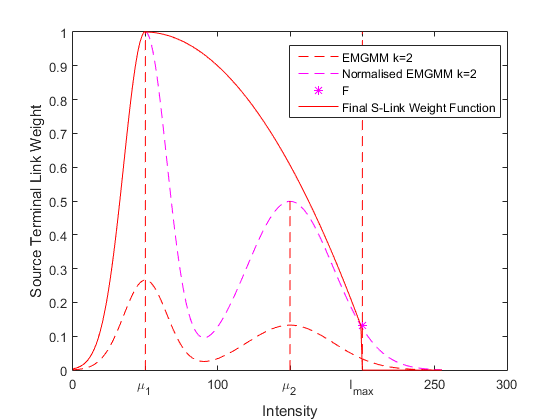
\includegraphics[scale=1]{/proposedinteractive/proposedinteractiveS}
		\caption{Object weighting function.}
		\label{fig:proposedinteractiveS}
	\end{figure}
\end{definition}


\begin{definition}[Background weighting function] 
	Similarly, the background weighting function is derived in the same way as the object weighting function. Let the maximum value of the intensity distribution be $k_{max} = P_{BG}$. Now $P_{BG}^{1} = \frac{P_{BG}}{k_{max}}$.
	
	Let the intensity value at which $P_{BG}^{1}$ is a maximum be denoted by $\iota_{BG}$. The intensity distribution before the point where the maximum value occurs is replaced by a parabola where the turning point maximum is $\left(\iota_{BG}, P_{BG}^{1}(\iota_{BG})\right)$ and the end point is $(0,B)$. The parabola defined by these points is 
	\begin{equation}
	P_{BG}^2(x) = \frac{B-1}{(\iota_{BG})^2}(x-\iota_{BG})^2 +1 
	\end{equation}
	where $x \in [0,\iota_{BG}]$.
	The final background weighitng function is
	\begin{equation}
	D_p("bkg") = \begin{cases} 
	P_{BG}^2(x) & x \in [0,\iota_{BG}) \\
	P_{BG}^1(x) & x \in [\iota_{BG},I_{max}]
	\end{cases}
	\end{equation}
	This function is plotted in \Cref{fig:proposedinteractiveT}.
	
	\textcolor{red}{Ensure that it obeys the submodularity constraint.}
	
	\begin{figure}[!h]
		\centering
		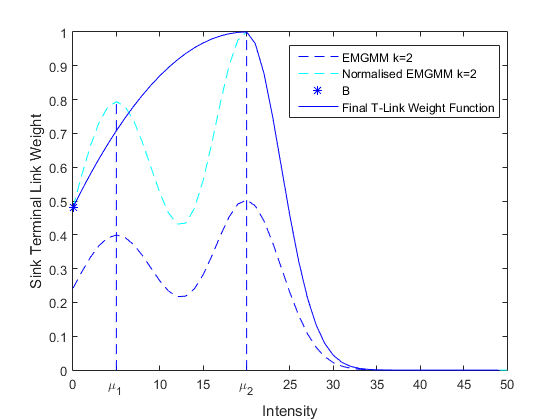
\includegraphics[scale=1]{/proposedinteractive/proposedinteractiveT}
		\caption{Background weighting function.}
		\label{fig:proposedinteractiveT}
	\end{figure}
\end{definition}

\begin{definition}[Hard Constraints]
	To enable the seeds marked by the user as hard constraints, we use the same technique in \citep{Boykov2001_2}. Background and object seeds are weighted using \Cref{eq:hardconstraintweight}.
\end{definition}



%----------------------------------------------------------------------------------------
%	SECTION 3
%----------------------------------------------------------------------------------------

\section{Determining Optimal Parameter Settings}
\label{sec:optimalparameters}

Although the weighting scheme presented by Eriksson \citep{Eriksson2006} and Boykov \citep{Boykov2001_2} are widely and probably one of the most common weighting schemes in use for interactive segmentation, there aren't any published parameters settings that work well specifically for fluorescent images. Therefore, we varied the tuning parameters for each weighting system and compared the segmentation results against the ground truth for the sample set in \Cref{fig:sampleset}. We ran the same test for the proposed scheme with and without hard constraints. We used the following parameter settings

\begin{align*}
	\lambda & = \{ 0.5, 1.25, 2.5, 5.0, 7.5, 10.0 \}\\
	\sigma & = \sigma_W = \{ 0.5, 1.25, 2.5, 5, 7.5 \}\\
	\sigma_R & = 1.
\end{align*}

To maintain as much commonality between the different weighting techniques we've used a common seed as illustrated in \Cref{fig:samplesetseed}. An extra seed is needed for the weighting systems by Eriksson \textit{et al.} and Boykov \textit{et al.} since, for all parameter settings, they were not able to register the cell nuclei as an object label. The results of the mean accuracy over the set for all parameter settings is plotted in \Cref{fig:interactiveweightingcomparison}. The parameter setting that performed the best is marked by a red asterisk. The optimal parameters over the range were found to be 

\begin{align*}
	( \lambda, \sigma_W, \sigma_R ) &= (10.0, 7.5, 1.0) & \text{Eriksson \textit{et al.}}\\
	( \lambda, \sigma) &= (7.5, 5.0) & \text{Boykov \textit{et al.}}\\
	( \lambda, \sigma) &= (0.5, 7.5) & \text{Proposed (No hard constraints)}\\
	( \lambda, \sigma) &= (0.5, 7.5) & \text{Proposed (Hard constraints)}
\end{align*}

The segmentation results with the optimal parameters for each weighting system is shown in \Cref{fig:interactivesampleseg1,fig:interactivesampleseg2,fig:interactivesampleseg3,fig:interactivesampleseg4,fig:interactivesampleseg5,fig:interactivesampleseg6}.

\begin{figure}[!h]
	\centering
	\subfigure[]
	{
		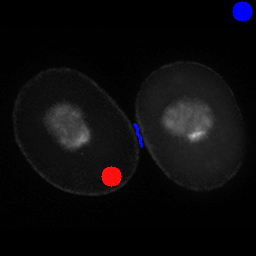
\includegraphics[width=0.23\columnwidth]{/proposedinteractive/sampleseeds/1seed}
		\label{fig:sampleseed1}
	}
	\subfigure[]
	{
		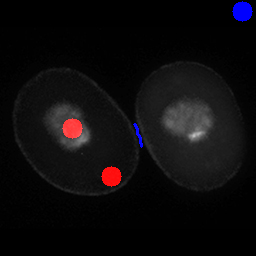
\includegraphics[width=0.23\columnwidth]{/proposedinteractive/sampleseeds/1seedboykov}
		\label{fig:sampleseed1b}
	}
	\subfigure[]
	{
		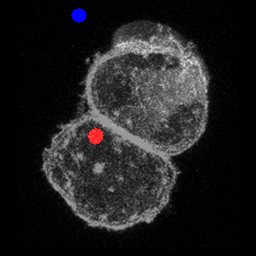
\includegraphics[width=0.23\columnwidth]{/proposedinteractive/sampleseeds/2seed}
		\label{fig:sampleseed2}
	}
	\subfigure[]
	{
		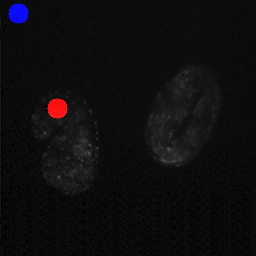
\includegraphics[width=0.23\columnwidth]{/proposedinteractive/sampleseeds/3seed}
		\label{fig:sampleseed3}
	}
	\subfigure[]
	{
		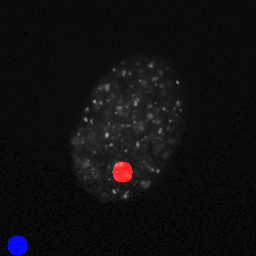
\includegraphics[width=0.23\columnwidth]{/proposedinteractive/sampleseeds/4seed}
		\label{fig:sampleseed4}
	}
	\subfigure[]
	{
		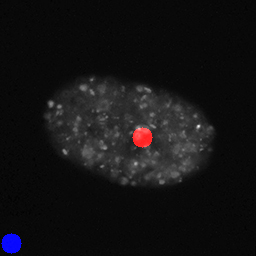
\includegraphics[width=0.23\columnwidth]{/proposedinteractive/sampleseeds/5seed}
		\label{fig:sampleseed5}
	}
	\subfigure[]
	{
		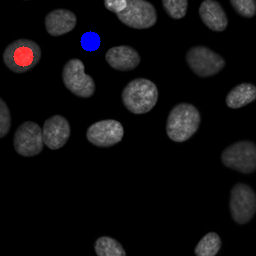
\includegraphics[width=0.23\columnwidth]{/proposedinteractive/sampleseeds/6seed}
		\label{fig:sampleseed6}
	}
	
	\caption{Seeds used over the sample set. The seeds for the first image differ in \textbf{(a)}, used for the proposed scheme, and \textbf{(b)} used for the weighting systems by Boykov and Eriksson as these were not able to grab the cell nuclei as part of the object.}
	\label{fig:samplesetseed}
\end{figure}

\begin{figure}[!t]
	\centering
	\subfigure[]
	{
		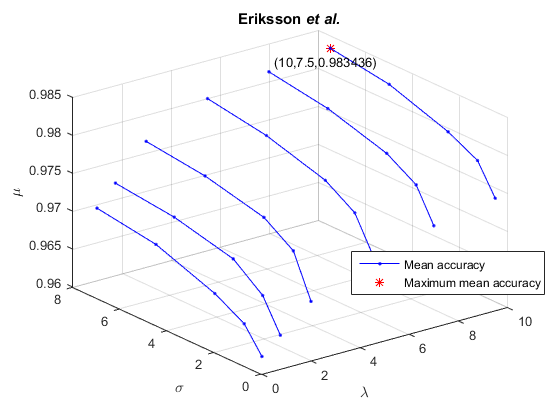
\includegraphics[width=0.48\columnwidth]{/proposedinteractive/eriksson}
		\label{fig:erikssoninteractive}
	}
	\subfigure[]
	{
		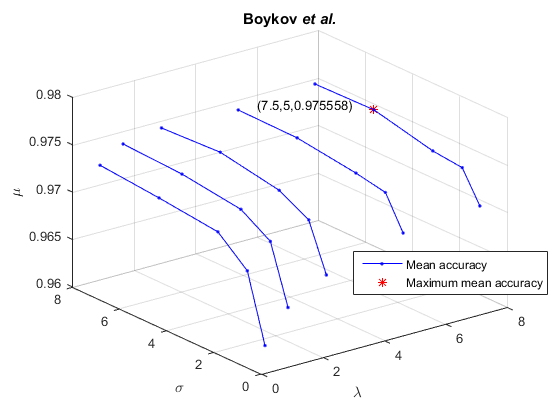
\includegraphics[width=0.48\columnwidth]{/proposedinteractive/boykov}
		\label{fig:boykovinteractive}
	}

	\subfigure[]
	{
		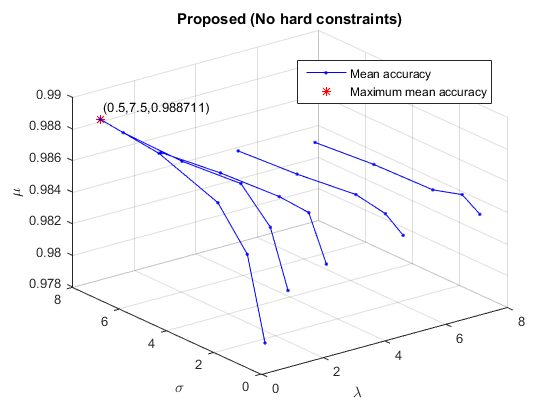
\includegraphics[width=0.48\columnwidth]{/proposedinteractive/proposed}
		\label{fig:proposedinteractive}
	}
	\subfigure[]
	{
		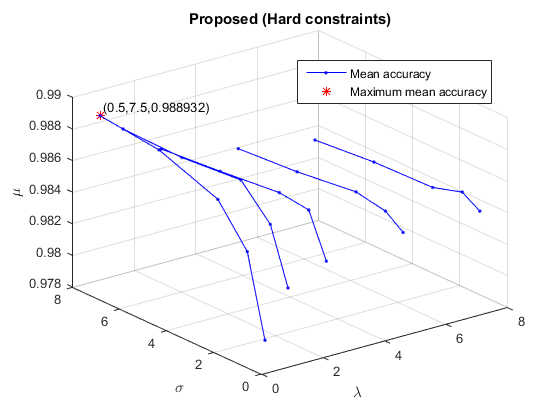
\includegraphics[width=0.48\columnwidth]{/proposedinteractive/proposedhc}
		\label{fig:proposedhcinteractive}
	}

	\caption{Plots of mean segmentation accuracy against the corresponding method tuning parameters.\textbf{(a)} Weighting system proposed by Eriksson \textit{et al.} The remaining parameter is set to $\sigma_R=1$. \textbf{(b)} Weighting system with hard constraints proposed by Boykov \textit{et al.} \textbf{(c)} Proposed weighting system without hard constraints. \textbf{(d)} Proposed weighting system with hard constraints.}
	\label{fig:interactiveweightingcomparison}
\end{figure}

\begin{figure}[!t]
	\centering
	\subfigure[]
	{
		\includegraphics[width=0.22\columnwidth]{/proposedinteractive/sampleeriksson/1seg}
		\label{fig:eriksson1}
	}
	\subfigure[]
	{
		\includegraphics[width=0.22\columnwidth]{/proposedinteractive/sampleboykov/1seg}
		\label{fig:boykov1}
	}
	\subfigure[]
	{
		\includegraphics[width=0.22\columnwidth]{/proposedinteractive/sampleproposed/1seg}
		\label{fig:proposed1}
	}
	\subfigure[]
	{
		\includegraphics[width=0.22\columnwidth]{/proposedinteractive/sampleproposedHC/1seg}
		\label{fig:proposedhc1}
	}
	
	\caption{Interactive segmentation of Image 1 in sample set (\Cref{fig:sampleset}). \textbf{(a)} Eriksson \textit{et al.} \textbf{(b)} Boykov \textit{et al.} \textbf{(c)} Proposed (No hard constraints) \textbf{(d)} Proposed with hard constraints.}
	\label{fig:interactivesampleseg1}
\end{figure}

\begin{figure}[!t]
	\centering
	\subfigure[]
	{
		\includegraphics[width=0.21\columnwidth]{/proposedinteractive/sampleeriksson/2seg}
		\label{fig:eriksson2}
	}
	\subfigure[]
	{
		\includegraphics[width=0.22\columnwidth]{/proposedinteractive/sampleboykov/2seg}
		\label{fig:boykov2}
	}
	\subfigure[]
	{
		\includegraphics[width=0.22\columnwidth]{/proposedinteractive/sampleproposed/2seg}
		\label{fig:proposed2}
	}
	\subfigure[]
	{
		\includegraphics[width=0.22\columnwidth]{/proposedinteractive/sampleproposedHC/2seg}
		\label{fig:proposedhc2}
	}
	
	\caption{Interactive segmentation of Image 2 in sample set (\Cref{fig:sampleset}). \textbf{(a)} Eriksson \textit{et al.} \textbf{(b)} Boykov \textit{et al.} \textbf{(c)} Proposed (No hard constraints) \textbf{(d)} Proposed with hard constraints.}
	\label{fig:interactivesampleseg2}
\end{figure}

\begin{figure}[!h]
	\centering
	\subfigure[]
	{
		\includegraphics[width=0.22\columnwidth]{/proposedinteractive/sampleeriksson/3seg}
		\label{fig:eriksson3}
	}
	\subfigure[]
	{
		\includegraphics[width=0.22\columnwidth]{/proposedinteractive/sampleboykov/3seg}
		\label{fig:boykov3}
	}
	\subfigure[]
	{
		\includegraphics[width=0.22\columnwidth]{/proposedinteractive/sampleproposed/3seg}
		\label{fig:proposed3}
	}
	\subfigure[]
	{
		\includegraphics[width=0.22\columnwidth]{/proposedinteractive/sampleproposedHC/3seg}
		\label{fig:proposedhc3}
	}
	
	\caption{Interactive segmentation of Image 3 in sample set (\Cref{fig:sampleset}). \textbf{(a)} Eriksson \textit{et al.} \textbf{(b)} Boykov \textit{et al.} \textbf{(c)} Proposed (No hard constraints) \textbf{(d)} Proposed with hard constraints.}
	\label{fig:interactivesampleseg3}
\end{figure}

\begin{figure}[!h]
	\centering
	\subfigure[]
	{
		\includegraphics[width=0.22\columnwidth]{/proposedinteractive/sampleeriksson/4seg}
		\label{fig:eriksson4}
	}
	\subfigure[]
	{
		\includegraphics[width=0.22\columnwidth]{/proposedinteractive/sampleboykov/4seg}
		\label{fig:boykov4}
	}
	\subfigure[]
	{
		\includegraphics[width=0.22\columnwidth]{/proposedinteractive/sampleproposed/4seg}
		\label{fig:proposed4}
	}
	\subfigure[]
	{
		\includegraphics[width=0.22\columnwidth]{/proposedinteractive/sampleproposedHC/4seg}
		\label{fig:proposedhc4}
	}
	
	\caption{Interactive segmentation of Image 4 in sample set (\Cref{fig:sampleset}). \textbf{(a)} Eriksson \textit{et al.} \textbf{(b)} Boykov \textit{et al.} \textbf{(c)} Proposed (No hard constraints) \textbf{(d)} Proposed with hard constraints.}
	\label{fig:interactivesampleseg4}
\end{figure}

\begin{figure}[!h]
	\centering
	\subfigure[]
	{
		\includegraphics[width=0.22\columnwidth]{/proposedinteractive/sampleeriksson/5seg}
		\label{fig:eriksson5}
	}
	\subfigure[]
	{
		\includegraphics[width=0.22\columnwidth]{/proposedinteractive/sampleboykov/5seg}
		\label{fig:boykov5}
	}
	\subfigure[]
	{
		\includegraphics[width=0.22\columnwidth]{/proposedinteractive/sampleproposed/5seg}
		\label{fig:proposed5}
	}
	\subfigure[]
	{
		\includegraphics[width=0.22\columnwidth]{/proposedinteractive/sampleproposedHC/5seg}
		\label{fig:proposedhc5}
	}
	
	\caption{Interactive segmentation of Image 5 in sample set (\Cref{fig:sampleset}). \textbf{(a)} Eriksson \textit{et al.} \textbf{(b)} Boykov \textit{et al.} \textbf{(c)} Proposed (No hard constraints) \textbf{(d)} Proposed with hard constraints.}
	\label{fig:interactivesampleseg5}
\end{figure}

\begin{figure}[!t]
	\centering
	\subfigure[]
	{
		\includegraphics[width=0.22\columnwidth]{/proposedinteractive/sampleeriksson/6seg}
		\label{fig:eriksson6}
	}
	\subfigure[]
	{
		\includegraphics[width=0.22\columnwidth]{/proposedinteractive/sampleboykov/6seg}
		\label{fig:boykov6}
	}
	\subfigure[]
	{
		\includegraphics[width=0.22\columnwidth]{/proposedinteractive/sampleproposed/6seg}
		\label{fig:proposed6}
	}
	\subfigure[]
	{
		\includegraphics[width=0.22\columnwidth]{/proposedinteractive/sampleproposedHC/6seg}
		\label{fig:proposedhc6}
	}
	
	\caption{Interactive segmentation of Image 6 in sample set (\Cref{fig:sampleset}). \textbf{(a)} Eriksson \textit{et al.} \textbf{(b)} Boykov \textit{et al.} \textbf{(c)} Proposed (No hard constraints) \textbf{(d)} Proposed with hard constraints.}
	\label{fig:interactivesampleseg6}
\end{figure}

%-----------------------------------
%	SECTION 4
%-----------------------------------
\clearpage
\section{Experimental Results}
\label{sec:interactiveresults}

We compared the segmentation results for optimal parameters found in \Cref{sec:optimalparameters}. We used a common seed for all images which is shown in \Cref{fig:188seed,fig:195seed,fig:228seed,fig:1057seed,fig:1265seed,fig:10093seed,fig:10102seed,fig:10104seed,fig:12294seed,fig:12627seed,fig:13432seed,fig:13438seed,fig:13899seed,fig:13901seed,fig:21749seed,fig:21759seed,fig:32140seed,fig:35278seed,fig:37338seed,fig:37339seed,fig:38974seed,fig:40217seed,fig:40968seed,fig:41066seed,fig:42451seed}. From the seeds we calculated a probability distribution based on EMGMM for $k=2$, each for the background and the object seeds.

The segmentation results where compared using the same method as in \Cref{sec:cvgc_experimentalresults}. That is, we've compiled a label for label comparison on the segmentation mask and the ground truth. The parameter settings with the corresponding segmentation results are shown in \Cref{tab:interactiveresults} including the efficiency measures \textit{precision}, \textit{recall}, \textit{accuracy} and \textit{Matthews Correlation Coefficient (MCC)}. The overview results are shown in \Cref{tab:overallinteractivesegmentationefficiency}. For each image we've highlighted the method which performs the best in blue and the worst in red.

We differentiate between methods on the same image as follows:

\textbf{[imageno]-[method]}, 

where \textit{imageno} goes from $1$ to $25$ and \textit{method} is defined as follows:
\begin{enumerate}
	\item [\textbf{e}] - using the optimal parameter setting for the weighting described by Eriksson \textit{et al.}
	\item [\textbf{b}] - using the optimal parameter setting for the weighting described by Boykov \textit{et al.}
	\item [\textbf{r1}] - Proposed method with optimal parameters found on the sample set.
	\item [\textbf{rh1}] - Proposed method with hard costraints for optimal parameters found on the sample set.
\end{enumerate}

\clearpage
%%%%%%%%%%%%%%%%%%%%%%%%%%%%%%%%%%%%%%%%%%%%%%%%%%%%%%%
% 188
\begin{figure}[!h]
	\centering
	\subfigure[Seeds.]
	{
		\includegraphics[width=0.23\columnwidth]{proposedinteractive/testseeds/188seg}
		\label{fig:188seed}
	}

	\subfigure[Eriksson \textit{et al.} $\lambda = 10$, $\sigma_W = 7.5$, $\sigma_R = 1$.]
	{
		\includegraphics[width=0.23\columnwidth]{proposedinteractive/testeriksson/188seg}
		\label{fig:eriksson188}
	}
	\subfigure[Boykov \textit{et al.} $\lambda=7.5$, $\sigma=5$.]
	{
		\includegraphics[width=0.23\columnwidth]{proposedinteractive/testboykov/188seg}
		\label{fig:boykov188}
	}
	\subfigure[Proposed $\lambda=0.5$, $\sigma=7.5$.]
	{
		\includegraphics[width=0.23\columnwidth]{proposedinteractive/testproposed/188seg}
		\label{fig:propsed188}
	}
	\subfigure[Proposed with hard constraints $\lambda=0.5$, $\sigma=7.5$.]
	{
		\includegraphics[width=0.23\columnwidth]{proposedinteractive/testproposedHC/188seg}
		\label{fig:propsedHC188}
	}
	\caption{Image 1 from test set \Cref{AppendixA} interactive segmentation results.}
	\label{fig:interactivetestresult188}
\end{figure}
%%%%%%%%%%%%%%%%%%%%%%%%%%%%%%%%%%%%%%%%%%%%%%%%%%%%%%%
% 195
\begin{figure}[!h]
	\centering
	\subfigure[Seeds.]
	{
		\includegraphics[width=0.23\columnwidth]{proposedinteractive/testseeds/195seg}
		\label{fig:195seed}
	}
	
	\subfigure[Eriksson \textit{et al.} $\lambda = 10$, $\sigma_W = 7.5$, $\sigma_R = 1$.]
	{
		\includegraphics[width=0.23\columnwidth]{proposedinteractive/testeriksson/195seg}
		\label{fig:eriksson195}
	}
	\subfigure[Boykov \textit{et al.} $\lambda=7.5$, $\sigma=5$.]
	{
		\includegraphics[width=0.23\columnwidth]{proposedinteractive/testboykov/195seg}
		\label{fig:boykov195}
	}
	\subfigure[Proposed $\lambda=0.5$, $\sigma=7.5$.]
	{
		\includegraphics[width=0.23\columnwidth]{proposedinteractive/testproposed/195seg}
		\label{fig:propsed195}
	}
	\subfigure[Proposed with hard constraints $\lambda=0.5$, $\sigma=7.5$.]
	{
		\includegraphics[width=0.23\columnwidth]{proposedinteractive/testproposedHC/195seg}
		\label{fig:propsedHC195}
	}
	\caption{Image 2 from test set \Cref{AppendixA} interactive segmentation results.}
	\label{fig:interactivetestresult195}
\end{figure}
%%%%%%%%%%%%%%%%%%%%%%%%%%%%%%%%%%%%%%%%%%%%%%%%%%%%%%%
% 228
\begin{figure}[!h]
	\centering
	\subfigure[Seeds.]
	{
		\includegraphics[width=0.23\columnwidth]{proposedinteractive/testseeds/228seg}
		\label{fig:228seed}
	}
	
	\subfigure[Eriksson \textit{et al.} $\lambda = 10$, $\sigma_W = 7.5$, $\sigma_R = 1$.]
	{
		\includegraphics[width=0.23\columnwidth]{proposedinteractive/testeriksson/228seg}
		\label{fig:eriksson228}
	}
	\subfigure[Boykov \textit{et al.} $\lambda=7.5$, $\sigma=5$.]
	{
		\includegraphics[width=0.23\columnwidth]{proposedinteractive/testboykov/228seg}
		\label{fig:boykov228}
	}
	\subfigure[Proposed $\lambda=0.5$, $\sigma=7.5$.]
	{
		\includegraphics[width=0.23\columnwidth]{proposedinteractive/testproposed/228seg}
		\label{fig:propsed228}
	}
	\subfigure[Proposed with hard constraints $\lambda=0.5$, $\sigma=7.5$.]
	{
		\includegraphics[width=0.23\columnwidth]{proposedinteractive/testproposedHC/228seg}
		\label{fig:propsedHC228}
	}
	\caption{Image 3 from test set \Cref{AppendixA} interactive segmentation results.}
	\label{fig:interactivetestresult228}
\end{figure}
%%%%%%%%%%%%%%%%%%%%%%%%%%%%%%%%%%%%%%%%%%%%%%%%%%%%%%%
% 1057
\begin{figure}[!h]
	\centering
	\subfigure[Seeds.]
	{
		\includegraphics[width=0.23\columnwidth]{proposedinteractive/testseeds/1057seg}
		\label{fig:1057seed}
	}
	
	\subfigure[Eriksson \textit{et al.} $\lambda = 10$, $\sigma_W = 7.5$, $\sigma_R = 1$.]
	{
		\includegraphics[width=0.23\columnwidth]{proposedinteractive/testeriksson/1057seg}
		\label{fig:eriksson1057}
	}
	\subfigure[Boykov \textit{et al.} $\lambda=7.5$, $\sigma=5$.]
	{
		\includegraphics[width=0.23\columnwidth]{proposedinteractive/testboykov/1057seg}
		\label{fig:boykov1057}
	}
	\subfigure[Proposed $\lambda=0.5$, $\sigma=7.5$.]
	{
		\includegraphics[width=0.23\columnwidth]{proposedinteractive/testproposed/1057seg}
		\label{fig:propsed1057}
	}
	\subfigure[Proposed with hard constraints $\lambda=0.5$, $\sigma=7.5$.]
	{
		\includegraphics[width=0.23\columnwidth]{proposedinteractive/testproposedHC/1057seg}
		\label{fig:propsedHC1057}
	}
	\caption{Image 4 from test set \Cref{AppendixA} interactive segmentation results.}
	\label{fig:interactivetestresult1057}
\end{figure}
%%%%%%%%%%%%%%%%%%%%%%%%%%%%%%%%%%%%%%%%%%%%%%%%%%%%%%%
% 1265
\begin{figure}[!h]
	\centering
	\subfigure[Seeds.]
	{
		\includegraphics[width=0.23\columnwidth]{proposedinteractive/testseeds/1265seg}
		\label{fig:1265seed}
	}
	
	\subfigure[Eriksson \textit{et al.} $\lambda = 10$, $\sigma_W = 7.5$, $\sigma_R = 1$.]
	{
		\includegraphics[width=0.23\columnwidth]{proposedinteractive/testeriksson/1265seg}
		\label{fig:eriksson1265}
	}
	\subfigure[Boykov \textit{et al.} $\lambda=7.5$, $\sigma=5$.]
	{
		\includegraphics[width=0.23\columnwidth]{proposedinteractive/testboykov/1265seg}
		\label{fig:boykov1265}
	}
	\subfigure[Proposed $\lambda=0.5$, $\sigma=7.5$.]
	{
		\includegraphics[width=0.23\columnwidth]{proposedinteractive/testproposed/1265seg}
		\label{fig:propsed1265}
	}
	\subfigure[Proposed with hard constraints $\lambda=0.5$, $\sigma=7.5$.]
	{
		\includegraphics[width=0.23\columnwidth]{proposedinteractive/testproposedHC/1265seg}
		\label{fig:propsedHC1265}
	}
	\caption{Image 5 from test set \Cref{AppendixA} interactive segmentation results.}
	\label{fig:interactivetestresult1265}
\end{figure}
%%%%%%%%%%%%%%%%%%%%%%%%%%%%%%%%%%%%%%%%%%%%%%%%%%%%%%%
% 10093
\begin{figure}[!h]
	\centering
	\subfigure[Seeds.]
	{
		\includegraphics[width=0.23\columnwidth]{proposedinteractive/testseeds/10093seg}
		\label{fig:10093seed}
	}
	
	\subfigure[Eriksson \textit{et al.} $\lambda = 10$, $\sigma_W = 7.5$, $\sigma_R = 1$.]
	{
		\includegraphics[width=0.23\columnwidth]{proposedinteractive/testeriksson/10093seg}
		\label{fig:eriksson10093}
	}
	\subfigure[Boykov \textit{et al.} $\lambda=7.5$, $\sigma=5$.]
	{
		\includegraphics[width=0.23\columnwidth]{proposedinteractive/testboykov/10093seg}
		\label{fig:boykov10093}
	}
	\subfigure[Proposed $\lambda=0.5$, $\sigma=7.5$.]
	{
		\includegraphics[width=0.23\columnwidth]{proposedinteractive/testproposed/10093seg}
		\label{fig:propsed10093}
	}
	\subfigure[Proposed with hard constraints $\lambda=0.5$, $\sigma=7.5$.]
	{
		\includegraphics[width=0.23\columnwidth]{proposedinteractive/testproposedHC/10093seg}
		\label{fig:propsedHC10093}
	}
	\caption{Image 6 from test set \Cref{AppendixA} interactive segmentation results.}
	\label{fig:interactivetestresult10093}
\end{figure}
%%%%%%%%%%%%%%%%%%%%%%%%%%%%%%%%%%%%%%%%%%%%%%%%%%%%%%%
% 10102
\begin{figure}[!h]
	\centering
	\subfigure[Seeds.]
	{
		\includegraphics[width=0.23\columnwidth]{proposedinteractive/testseeds/10102seg}
		\label{fig:10102seed}
	}
	
	\subfigure[Eriksson \textit{et al.} $\lambda = 10$, $\sigma_W = 7.5$, $\sigma_R = 1$.]
	{
		\includegraphics[width=0.23\columnwidth]{proposedinteractive/testeriksson/10102seg}
		\label{fig:eriksson10102}
	}
	\subfigure[Boykov \textit{et al.} $\lambda=7.5$, $\sigma=5$.]
	{
		\includegraphics[width=0.23\columnwidth]{proposedinteractive/testboykov/10102seg}
		\label{fig:boykov10102}
	}
	\subfigure[Proposed $\lambda=0.5$, $\sigma=7.5$.]
	{
		\includegraphics[width=0.23\columnwidth]{proposedinteractive/testproposed/10102seg}
		\label{fig:propsed10102}
	}
	\subfigure[Proposed with hard constraints $\lambda=0.5$, $\sigma=7.5$.]
	{
		\includegraphics[width=0.23\columnwidth]{proposedinteractive/testproposedHC/10102seg}
		\label{fig:propsedHC10102}
	}
	\caption{Image 7 from test set \Cref{AppendixA} interactive segmentation results.}
	\label{fig:interactivetestresult10102}
\end{figure}
%%%%%%%%%%%%%%%%%%%%%%%%%%%%%%%%%%%%%%%%%%%%%%%%%%%%%%%
% 10104
\begin{figure}[!h]
	\centering
	\subfigure[Seeds.]
	{
		\includegraphics[width=0.23\columnwidth]{proposedinteractive/testseeds/10104seg}
		\label{fig:10104seed}
	}
	
	\subfigure[Eriksson \textit{et al.} $\lambda = 10$, $\sigma_W = 7.5$, $\sigma_R = 1$.]
	{
		\includegraphics[width=0.23\columnwidth]{proposedinteractive/testeriksson/10104seg}
		\label{fig:eriksson10104}
	}
	\subfigure[Boykov \textit{et al.} $\lambda=7.5$, $\sigma=5$.]
	{
		\includegraphics[width=0.23\columnwidth]{proposedinteractive/testboykov/10104seg}
		\label{fig:boykov10104}
	}
	\subfigure[Proposed $\lambda=0.5$, $\sigma=7.5$.]
	{
		\includegraphics[width=0.23\columnwidth]{proposedinteractive/testproposed/10104seg}
		\label{fig:propsed10104}
	}
	\subfigure[Proposed with hard constraints $\lambda=0.5$, $\sigma=7.5$.]
	{
		\includegraphics[width=0.23\columnwidth]{proposedinteractive/testproposedHC/10104seg}
		\label{fig:propsedHC10104}
	}
	\caption{Image 8 from test set \Cref{AppendixA} interactive segmentation results.}
	\label{fig:interactivetestresult10104}
\end{figure}
%%%%%%%%%%%%%%%%%%%%%%%%%%%%%%%%%%%%%%%%%%%%%%%%%%%%%%%
% 12294
\begin{figure}[!h]
	\centering
	\subfigure[Seeds.]
	{
		\includegraphics[width=0.23\columnwidth]{proposedinteractive/testseeds/12294seg}
		\label{fig:12294seed}
	}
	
	\subfigure[Eriksson \textit{et al.} $\lambda = 10$, $\sigma_W = 7.5$, $\sigma_R = 1$.]
	{
		\includegraphics[width=0.23\columnwidth]{proposedinteractive/testeriksson/12294seg}
		\label{fig:eriksson12294}
	}
	\subfigure[Boykov \textit{et al.} $\lambda=7.5$, $\sigma=5$.]
	{
		\includegraphics[width=0.23\columnwidth]{proposedinteractive/testboykov/12294seg}
		\label{fig:boykov12294}
	}
	\subfigure[Proposed $\lambda=0.5$, $\sigma=7.5$.]
	{
		\includegraphics[width=0.23\columnwidth]{proposedinteractive/testproposed/12294seg}
		\label{fig:propsed12294}
	}
	\subfigure[Proposed with hard constraints $\lambda=0.5$, $\sigma=7.5$.]
	{
		\includegraphics[width=0.23\columnwidth]{proposedinteractive/testproposedHC/12294seg}
		\label{fig:propsedHC12294}
	}
	\caption{Image 9 from test set \Cref{AppendixA} interactive segmentation results.}
	\label{fig:interactivetestresult12294}
\end{figure}
%%%%%%%%%%%%%%%%%%%%%%%%%%%%%%%%%%%%%%%%%%%%%%%%%%%%%%%
% 12627
\begin{figure}[!h]
	\centering
	\subfigure[Seeds.]
	{
		\includegraphics[width=0.23\columnwidth]{proposedinteractive/testseeds/12627seg}
		\label{fig:12627seed}
	}
	
	\subfigure[Eriksson \textit{et al.} $\lambda = 10$, $\sigma_W = 7.5$, $\sigma_R = 1$.]
	{
		\includegraphics[width=0.23\columnwidth]{proposedinteractive/testeriksson/12627seg}
		\label{fig:eriksson12627}
	}
	\subfigure[Boykov \textit{et al.} $\lambda=7.5$, $\sigma=5$.]
	{
		\includegraphics[width=0.23\columnwidth]{proposedinteractive/testboykov/12627seg}
		\label{fig:boykov12627}
	}
	\subfigure[Proposed $\lambda=0.5$, $\sigma=7.5$.]
	{
		\includegraphics[width=0.23\columnwidth]{proposedinteractive/testproposed/12627seg}
		\label{fig:propsed12627}
	}
	\subfigure[Proposed with hard constraints $\lambda=0.5$, $\sigma=7.5$.]
	{
		\includegraphics[width=0.23\columnwidth]{proposedinteractive/testproposedHC/12627seg}
		\label{fig:propsedHC12627}
	}
	\caption{Image 10 from test set \Cref{AppendixA} interactive segmentation results.}
	\label{fig:interactivetestresult12627}
\end{figure}
%%%%%%%%%%%%%%%%%%%%%%%%%%%%%%%%%%%%%%%%%%%%%%%%%%%%%%%
% 13432
\begin{figure}[!h]
	\centering
	\subfigure[Seeds.]
	{
		\includegraphics[width=0.23\columnwidth]{proposedinteractive/testseeds/13432seg}
		\label{fig:13432seed}
	}
	
	\subfigure[Eriksson \textit{et al.} $\lambda = 10$, $\sigma_W = 7.5$, $\sigma_R = 1$.]
	{
		\includegraphics[width=0.23\columnwidth]{proposedinteractive/testeriksson/13432seg}
		\label{fig:eriksson13432}
	}
	\subfigure[Boykov \textit{et al.} $\lambda=7.5$, $\sigma=5$.]
	{
		\includegraphics[width=0.23\columnwidth]{proposedinteractive/testboykov/13432seg}
		\label{fig:boykov13432}
	}
	\subfigure[Proposed $\lambda=0.5$, $\sigma=7.5$.]
	{
		\includegraphics[width=0.23\columnwidth]{proposedinteractive/testproposed/13432seg}
		\label{fig:propsed13432}
	}
	\subfigure[Proposed with hard constraints $\lambda=0.5$, $\sigma=7.5$.]
	{
		\includegraphics[width=0.23\columnwidth]{proposedinteractive/testproposedHC/13432seg}
		\label{fig:propsedHC13432}
	}
	\caption{Image 11 from test set \Cref{AppendixA} interactive segmentation results.}
	\label{fig:interactivetestresult13432}
\end{figure}
%%%%%%%%%%%%%%%%%%%%%%%%%%%%%%%%%%%%%%%%%%%%%%%%%%%%%%%
% 13438
\begin{figure}[!h]
	\centering
	\subfigure[Seeds.]
	{
		\includegraphics[width=0.23\columnwidth]{proposedinteractive/testseeds/13438seg}
		\label{fig:13438seed}
	}
	
	\subfigure[Eriksson \textit{et al.} $\lambda = 10$, $\sigma_W = 7.5$, $\sigma_R = 1$.]
	{
		\includegraphics[width=0.23\columnwidth]{proposedinteractive/testeriksson/13438seg}
		\label{fig:eriksson13438}
	}
	\subfigure[Boykov \textit{et al.} $\lambda=7.5$, $\sigma=5$.]
	{
		\includegraphics[width=0.23\columnwidth]{proposedinteractive/testboykov/13438seg}
		\label{fig:boykov13438}
	}
	\subfigure[Proposed $\lambda=0.5$, $\sigma=7.5$.]
	{
		\includegraphics[width=0.23\columnwidth]{proposedinteractive/testproposed/13438seg}
		\label{fig:propsed13438}
	}
	\subfigure[Proposed with hard constraints $\lambda=0.5$, $\sigma=7.5$.]
	{
		\includegraphics[width=0.23\columnwidth]{proposedinteractive/testproposedHC/13438seg}
		\label{fig:propsedHC13438}
	}
	\caption{Image 12 from test set \Cref{AppendixA} interactive segmentation results.}
	\label{fig:interactivetestresult13438}
\end{figure}
%%%%%%%%%%%%%%%%%%%%%%%%%%%%%%%%%%%%%%%%%%%%%%%%%%%%%%%
% 13899
\begin{figure}[!h]
	\centering
	\subfigure[Seeds.]
	{
		\includegraphics[width=0.23\columnwidth]{proposedinteractive/testseeds/13899seg}
		\label{fig:13899seed}
	}
	
	\subfigure[Eriksson \textit{et al.} $\lambda = 10$, $\sigma_W = 7.5$, $\sigma_R = 1$.]
	{
		\includegraphics[width=0.23\columnwidth]{proposedinteractive/testeriksson/13899seg}
		\label{fig:eriksson13899}
	}
	\subfigure[Boykov \textit{et al.} $\lambda=7.5$, $\sigma=5$.]
	{
		\includegraphics[width=0.23\columnwidth]{proposedinteractive/testboykov/13899seg}
		\label{fig:boykov13899}
	}
	\subfigure[Proposed $\lambda=0.5$, $\sigma=7.5$.]
	{
		\includegraphics[width=0.23\columnwidth]{proposedinteractive/testproposed/13899seg}
		\label{fig:propsed13899}
	}
	\subfigure[Proposed with hard constraints $\lambda=0.5$, $\sigma=7.5$.]
	{
		\includegraphics[width=0.23\columnwidth]{proposedinteractive/testproposedHC/13899seg}
		\label{fig:propsedHC13899}
	}
	\caption{Image 13 from test set \Cref{AppendixA} interactive segmentation results.}
	\label{fig:interactivetestresult13899}
\end{figure}
%%%%%%%%%%%%%%%%%%%%%%%%%%%%%%%%%%%%%%%%%%%%%%%%%%%%%%%
% 13901
\begin{figure}[!h]
	\centering
	\subfigure[Seeds.]
	{
		\includegraphics[width=0.23\columnwidth]{proposedinteractive/testseeds/13901seg}
		\label{fig:13901seed}
	}
	
	\subfigure[Eriksson \textit{et al.} $\lambda = 10$, $\sigma_W = 7.5$, $\sigma_R = 1$.]
	{
		\includegraphics[width=0.23\columnwidth]{proposedinteractive/testeriksson/13901seg}
		\label{fig:eriksson13901}
	}
	\subfigure[Boykov \textit{et al.} $\lambda=7.5$, $\sigma=5$.]
	{
		\includegraphics[width=0.23\columnwidth]{proposedinteractive/testboykov/13901seg}
		\label{fig:boykov13901}
	}
	\subfigure[Proposed $\lambda=0.5$, $\sigma=7.5$.]
	{
		\includegraphics[width=0.23\columnwidth]{proposedinteractive/testproposed/13901seg}
		\label{fig:propsed13901}
	}
	\subfigure[Proposed with hard constraints $\lambda=0.5$, $\sigma=7.5$.]
	{
		\includegraphics[width=0.23\columnwidth]{proposedinteractive/testproposedHC/13901seg}
		\label{fig:propsedHC13901}
	}
	\caption{Image 14 from test set \Cref{AppendixA} interactive segmentation results.}
	\label{fig:interactivetestresult13901}
\end{figure}
%%%%%%%%%%%%%%%%%%%%%%%%%%%%%%%%%%%%%%%%%%%%%%%%%%%%%%%
% 21749
\begin{figure}[!h]
	\centering
	\subfigure[Seeds.]
	{
		\includegraphics[width=0.23\columnwidth]{proposedinteractive/testseeds/21749seg}
		\label{fig:21749seed}
	}
	
	\subfigure[Eriksson \textit{et al.} $\lambda = 10$, $\sigma_W = 7.5$, $\sigma_R = 1$.]
	{
		\includegraphics[width=0.23\columnwidth]{proposedinteractive/testeriksson/21749seg}
		\label{fig:eriksson21749}
	}
	\subfigure[Boykov \textit{et al.} $\lambda=7.5$, $\sigma=5$.]
	{
		\includegraphics[width=0.23\columnwidth]{proposedinteractive/testboykov/21749seg}
		\label{fig:boykov21749}
	}
	\subfigure[Proposed $\lambda=0.5$, $\sigma=7.5$.]
	{
		\includegraphics[width=0.23\columnwidth]{proposedinteractive/testproposed/21749seg}
		\label{fig:propsed21749}
	}
	\subfigure[Proposed with hard constraints $\lambda=0.5$, $\sigma=7.5$.]
	{
		\includegraphics[width=0.23\columnwidth]{proposedinteractive/testproposedHC/21749seg}
		\label{fig:propsedHC21749}
	}
	\caption{Image 15 from test set \Cref{AppendixA} interactive segmentation results.}
	\label{fig:interactivetestresult21749}
\end{figure}
%%%%%%%%%%%%%%%%%%%%%%%%%%%%%%%%%%%%%%%%%%%%%%%%%%%%%%%
% 21759
\begin{figure}[!h]
	\centering
	\subfigure[Seeds.]
	{
		\includegraphics[width=0.23\columnwidth]{proposedinteractive/testseeds/21759seg}
		\label{fig:21759seed}
	}
	
	\subfigure[Eriksson \textit{et al.} $\lambda = 10$, $\sigma_W = 7.5$, $\sigma_R = 1$.]
	{
		\includegraphics[width=0.23\columnwidth]{proposedinteractive/testeriksson/21759seg}
		\label{fig:eriksson21759}
	}
	\subfigure[Boykov \textit{et al.} $\lambda=7.5$, $\sigma=5$.]
	{
		\includegraphics[width=0.23\columnwidth]{proposedinteractive/testboykov/21759seg}
		\label{fig:boykov21759}
	}
	\subfigure[Proposed $\lambda=0.5$, $\sigma=7.5$.]
	{
		\includegraphics[width=0.23\columnwidth]{proposedinteractive/testproposed/21759seg}
		\label{fig:propsed21759}
	}
	\subfigure[Proposed with hard constraints $\lambda=0.5$, $\sigma=7.5$.]
	{
		\includegraphics[width=0.23\columnwidth]{proposedinteractive/testproposedHC/21759seg}
		\label{fig:propsedHC21759}
	}
	\caption{Image 16 from test set \Cref{AppendixA} interactive segmentation results.}
	\label{fig:interactivetestresult21759}
\end{figure}
%%%%%%%%%%%%%%%%%%%%%%%%%%%%%%%%%%%%%%%%%%%%%%%%%%%%%%%
% 32140
\begin{figure}[!h]
	\centering
	\subfigure[Seeds.]
	{
		\includegraphics[width=0.23\columnwidth]{proposedinteractive/testseeds/32140seg}
		\label{fig:32140seed}
	}
	
	\subfigure[Eriksson \textit{et al.} $\lambda = 10$, $\sigma_W = 7.5$, $\sigma_R = 1$.]
	{
		\includegraphics[width=0.23\columnwidth]{proposedinteractive/testeriksson/32140seg}
		\label{fig:eriksson32140}
	}
	\subfigure[Boykov \textit{et al.} $\lambda=7.5$, $\sigma=5$.]
	{
		\includegraphics[width=0.23\columnwidth]{proposedinteractive/testboykov/32140seg}
		\label{fig:boykov32140}
	}
	\subfigure[Proposed $\lambda=0.5$, $\sigma=7.5$.]
	{
		\includegraphics[width=0.23\columnwidth]{proposedinteractive/testproposed/32140seg}
		\label{fig:propsed32140}
	}
	\subfigure[Proposed with hard constraints $\lambda=0.5$, $\sigma=7.5$.]
	{
		\includegraphics[width=0.23\columnwidth]{proposedinteractive/testproposedHC/32140seg}
		\label{fig:propsedHC32140}
	}
	\caption{Image 17 from test set \Cref{AppendixA} interactive segmentation results.}
	\label{fig:interactivetestresult32140}
\end{figure}
%%%%%%%%%%%%%%%%%%%%%%%%%%%%%%%%%%%%%%%%%%%%%%%%%%%%%%%
% 35278
\begin{figure}[!h]
	\centering
	\subfigure[Seeds.]
	{
		\includegraphics[width=0.23\columnwidth]{proposedinteractive/testseeds/35278seg}
		\label{fig:35278seed}
	}
	
	\subfigure[Eriksson \textit{et al.} $\lambda = 10$, $\sigma_W = 7.5$, $\sigma_R = 1$.]
	{
		\includegraphics[width=0.23\columnwidth]{proposedinteractive/testeriksson/35278seg}
		\label{fig:eriksson35278}
	}
	\subfigure[Boykov \textit{et al.} $\lambda=7.5$, $\sigma=5$.]
	{
		\includegraphics[width=0.23\columnwidth]{proposedinteractive/testboykov/35278seg}
		\label{fig:boykov35278}
	}
	\subfigure[Proposed $\lambda=0.5$, $\sigma=7.5$.]
	{
		\includegraphics[width=0.23\columnwidth]{proposedinteractive/testproposed/35278seg}
		\label{fig:propsed35278}
	}
	\subfigure[Proposed with hard constraints $\lambda=0.5$, $\sigma=7.5$.]
	{
		\includegraphics[width=0.23\columnwidth]{proposedinteractive/testproposedHC/35278seg}
		\label{fig:propsedHC35278}
	}
	\caption{Image 18 from test set \Cref{AppendixA} interactive segmentation results.}
	\label{fig:interactivetestresult35278}
\end{figure}
%%%%%%%%%%%%%%%%%%%%%%%%%%%%%%%%%%%%%%%%%%%%%%%%%%%%%%%
% 37338
\begin{figure}[!h]
	\centering
	\subfigure[Seeds.]
	{
		\includegraphics[width=0.23\columnwidth]{proposedinteractive/testseeds/37338seg}
		\label{fig:37338seed}
	}
	
	\subfigure[Eriksson \textit{et al.} $\lambda = 10$, $\sigma_W = 7.5$, $\sigma_R = 1$.]
	{
		\includegraphics[width=0.23\columnwidth]{proposedinteractive/testeriksson/37338seg}
		\label{fig:eriksson37338}
	}
	\subfigure[Boykov \textit{et al.} $\lambda=7.5$, $\sigma=5$.]
	{
		\includegraphics[width=0.23\columnwidth]{proposedinteractive/testboykov/37338seg}
		\label{fig:boykov37338}
	}
	\subfigure[Proposed $\lambda=0.5$, $\sigma=7.5$.]
	{
		\includegraphics[width=0.23\columnwidth]{proposedinteractive/testproposed/37338seg}
		\label{fig:propsed37338}
	}
	\subfigure[Proposed with hard constraints $\lambda=0.5$, $\sigma=7.5$.]
	{
		\includegraphics[width=0.23\columnwidth]{proposedinteractive/testproposedHC/37338seg}
		\label{fig:propsedHC37338}
	}
	\caption{Image 19 from test set \Cref{AppendixA} interactive segmentation results.}
	\label{fig:interactivetestresult37338}
\end{figure}
%%%%%%%%%%%%%%%%%%%%%%%%%%%%%%%%%%%%%%%%%%%%%%%%%%%%%%%
% 37339
\begin{figure}[!h]
\centering
\subfigure[Seeds.]
{
	\includegraphics[width=0.23\columnwidth]{proposedinteractive/testseeds/37339seg}
	\label{fig:37339seed}
}

\subfigure[Eriksson \textit{et al.} $\lambda = 10$, $\sigma_W = 7.5$, $\sigma_R = 1$.]
{
	\includegraphics[width=0.23\columnwidth]{proposedinteractive/testeriksson/37339seg}
	\label{fig:eriksson37339}
}
\subfigure[Boykov \textit{et al.} $\lambda=7.5$, $\sigma=5$.]
{
	\includegraphics[width=0.23\columnwidth]{proposedinteractive/testboykov/37339seg}
	\label{fig:boykov37339}
}
\subfigure[Proposed $\lambda=0.5$, $\sigma=7.5$.]
{
	\includegraphics[width=0.23\columnwidth]{proposedinteractive/testproposed/37339seg}
	\label{fig:propsed37339}
}
\subfigure[Proposed with hard constraints $\lambda=0.5$, $\sigma=7.5$.]
{
	\includegraphics[width=0.23\columnwidth]{proposedinteractive/testproposedHC/37339seg}
	\label{fig:propsedHC37339}
}
\caption{Image 20 from test set \Cref{AppendixA} interactive segmentation results.}
\label{fig:interactivetestresult37339}
\end{figure}
%%%%%%%%%%%%%%%%%%%%%%%%%%%%%%%%%%%%%%%%%%%%%%%%%%%%%%%
% 38974
\begin{figure}[!h]
	\centering
	\subfigure[Seeds.]
	{
		\includegraphics[width=0.23\columnwidth]{proposedinteractive/testseeds/38974seg}
		\label{fig:38974seed}
	}
	
	\subfigure[Eriksson \textit{et al.} $\lambda = 10$, $\sigma_W = 7.5$, $\sigma_R = 1$.]
	{
		\includegraphics[width=0.23\columnwidth]{proposedinteractive/testeriksson/38974seg}
		\label{fig:eriksson38974}
	}
	\subfigure[Boykov \textit{et al.} $\lambda=7.5$, $\sigma=5$.]
	{
		\includegraphics[width=0.23\columnwidth]{proposedinteractive/testboykov/38974seg}
		\label{fig:boykov38974}
	}
	\subfigure[Proposed $\lambda=0.5$, $\sigma=7.5$.]
	{
		\includegraphics[width=0.23\columnwidth]{proposedinteractive/testproposed/38974seg}
		\label{fig:propsed38974}
	}
	\subfigure[Proposed with hard constraints $\lambda=0.5$, $\sigma=7.5$.]
	{
		\includegraphics[width=0.23\columnwidth]{proposedinteractive/testproposedHC/38974seg}
		\label{fig:propsedHC38974}
	}
	\caption{Image 21 from test set \Cref{AppendixA} interactive segmentation results.}
	\label{fig:interactivetestresult38974}
\end{figure}
%%%%%%%%%%%%%%%%%%%%%%%%%%%%%%%%%%%%%%%%%%%%%%%%%%%%%%%
% 40217
\begin{figure}[!h]
	\centering
	\subfigure[Seeds.]
	{
		\includegraphics[width=0.23\columnwidth]{proposedinteractive/testseeds/40217seg}
		\label{fig:40217seed}
	}
	
	\subfigure[Eriksson \textit{et al.} $\lambda = 10$, $\sigma_W = 7.5$, $\sigma_R = 1$.]
	{
		\includegraphics[width=0.23\columnwidth]{proposedinteractive/testeriksson/40217seg}
		\label{fig:eriksson40217}
	}
	\subfigure[Boykov \textit{et al.} $\lambda=7.5$, $\sigma=5$.]
	{
		\includegraphics[width=0.23\columnwidth]{proposedinteractive/testboykov/40217seg}
		\label{fig:boykov40217}
	}
	\subfigure[Proposed $\lambda=0.5$, $\sigma=7.5$.]
	{
		\includegraphics[width=0.23\columnwidth]{proposedinteractive/testproposed/40217seg}
		\label{fig:propsed40217}
	}
	\subfigure[Proposed with hard constraints $\lambda=0.5$, $\sigma=7.5$.]
	{
		\includegraphics[width=0.23\columnwidth]{proposedinteractive/testproposedHC/40217seg}
		\label{fig:propsedHC40217}
	}
	\caption{Image 22 from test set \Cref{AppendixA} interactive segmentation results.}
	\label{fig:interactivetestresult40217}
\end{figure}
%%%%%%%%%%%%%%%%%%%%%%%%%%%%%%%%%%%%%%%%%%%%%%%%%%%%%%%
% 40968
\begin{figure}[!h]
	\centering
	\subfigure[Seeds.]
	{
		\includegraphics[width=0.23\columnwidth]{proposedinteractive/testseeds/40968seg}
		\label{fig:40968seed}
	}
	
	\subfigure[Eriksson \textit{et al.} $\lambda = 10$, $\sigma_W = 7.5$, $\sigma_R = 1$.]
	{
		\includegraphics[width=0.23\columnwidth]{proposedinteractive/testeriksson/40968seg}
		\label{fig:eriksson40968}
	}
	\subfigure[Boykov \textit{et al.} $\lambda=7.5$, $\sigma=5$.]
	{
		\includegraphics[width=0.23\columnwidth]{proposedinteractive/testboykov/40968seg}
		\label{fig:boykov40968}
	}
	\subfigure[Proposed $\lambda=0.5$, $\sigma=7.5$.]
	{
		\includegraphics[width=0.23\columnwidth]{proposedinteractive/testproposed/40968seg}
		\label{fig:propsed40968}
	}
	\subfigure[Proposed with hard constraints $\lambda=0.5$, $\sigma=7.5$.]
	{
		\includegraphics[width=0.23\columnwidth]{proposedinteractive/testproposedHC/40968seg}
		\label{fig:propsedHC40968}
	}
	\caption{Image 23 from test set \Cref{AppendixA} interactive segmentation results.}
	\label{fig:interactivetestresult40968}
\end{figure}
%%%%%%%%%%%%%%%%%%%%%%%%%%%%%%%%%%%%%%%%%%%%%%%%%%%%%%%
% 41066
\begin{figure}[!h]
	\centering
	\subfigure[Seeds.]
	{
		\includegraphics[width=0.23\columnwidth]{proposedinteractive/testseeds/41066seg}
		\label{fig:41066seed}
	}
	
	\subfigure[Eriksson \textit{et al.} $\lambda = 10$, $\sigma_W = 7.5$, $\sigma_R = 1$.]
	{
		\includegraphics[width=0.23\columnwidth]{proposedinteractive/testeriksson/41066seg}
		\label{fig:eriksson41066}
	}
	\subfigure[Boykov \textit{et al.} $\lambda=7.5$, $\sigma=5$.]
	{
		\includegraphics[width=0.23\columnwidth]{proposedinteractive/testboykov/41066seg}
		\label{fig:boykov41066}
	}
	\subfigure[Proposed $\lambda=0.5$, $\sigma=7.5$.]
	{
		\includegraphics[width=0.23\columnwidth]{proposedinteractive/testproposed/41066seg}
		\label{fig:propsed41066}
	}
	\subfigure[Proposed with hard constraints $\lambda=0.5$, $\sigma=7.5$.]
	{
		\includegraphics[width=0.23\columnwidth]{proposedinteractive/testproposedHC/41066seg}
		\label{fig:propsedHC41066}
	}
	\caption{Image 24 from test set \Cref{AppendixA} interactive segmentation results.}
	\label{fig:interactivetestresult41066}
\end{figure}
%%%%%%%%%%%%%%%%%%%%%%%%%%%%%%%%%%%%%%%%%%%%%%%%%%%%%%%
% 42451
\begin{figure}[!h]
	\centering
	\subfigure[Seeds.]
	{
		\includegraphics[width=0.23\columnwidth]{proposedinteractive/testseeds/42451seg}
		\label{fig:42451seed}
	}
	
	\subfigure[Eriksson \textit{et al.} $\lambda = 10$, $\sigma_W = 7.5$, $\sigma_R = 1$.]
	{
		\includegraphics[width=0.23\columnwidth]{proposedinteractive/testeriksson/42451seg}
		\label{fig:eriksson42451}
	}
	\subfigure[Boykov \textit{et al.} $\lambda=7.5$, $\sigma=5$.]
	{
		\includegraphics[width=0.23\columnwidth]{proposedinteractive/testboykov/42451seg}
		\label{fig:boykov42451}
	}
	\subfigure[Proposed $\lambda=0.5$, $\sigma=7.5$.]
	{
		\includegraphics[width=0.23\columnwidth]{proposedinteractive/testproposed/42451seg}
		\label{fig:propsed42451}
	}
	\subfigure[Proposed with hard constraints $\lambda=0.5$, $\sigma=7.5$.]
	{
		\includegraphics[width=0.23\columnwidth]{proposedinteractive/testproposedHC/42451seg}
		\label{fig:propsedHC42451}
	}
	\caption{Image 25 from test set \Cref{AppendixA} interactive segmentation results.}
	\label{fig:interactivetestresult42451}
\end{figure}

\clearpage
\begin{longtable}[!h]{|c|c|c|c|c|c|c|c|c|}
	\caption{Interactive segmentation results.} \label{tab:interactiveresults}\\
	\hline	Image	&	TP	&	TN	&	FP	&	FN	&	Precision	&	Recall	&	Accuracy	&	MCC	\\
	\hline \rowcolor{closest} 1-e	&	39901	&	24637	&	879	&	119	&	0.978445	&	0.997026	&	0.984772	&	0.968092	\\
	\hline \rowcolor{bad}	1-b	&	40020	&	23280	&	2236	&	0	&	0.947084	&	1.000000	&	0.965881	&	0.929565	\\
	\hline	1-r1	&	38125	&	25489	&	27	&	1895	&	0.999292	&	0.952649	&	0.970673	&	0.940780	\\
	\hline	1-rh1	&	38125	&	25489	&	27	&	1895	&	0.999292	&	0.952649	&	0.970673	&	0.940780	\\
	
	\hline \rowcolor{closest} 2-e	&	20880	&	40848	&	2742	&	1066	&	0.883922	&	0.951426	&	0.941895	&	0.873376	\\
	\hline	2-b	&	20417	&	40801	&	2789	&	1529	&	0.879816	&	0.930329	&	0.934113	&	0.854946	\\
	\hline \rowcolor{bad}	2-r1	&	21798	&	38965	&	4625	&	148	&	0.824963	&	0.993256	&	0.927170	&	0.853529	\\
	\hline \rowcolor{bad}	2-rh1	&	21798	&	38965	&	4625	&	148	&	0.824963	&	0.993256	&	0.927170	&	0.853529	\\
	
	\hline	3-e	&	10043	&	55027	&	404	&	62	&	0.961329	&	0.993864	&	0.992889	&	0.973300	\\
	\hline \rowcolor{closest}	3-b	&	10105	&	55056	&	375	&	0	&	0.964218	&	1.000000	&	0.994278	&	0.978619	\\
	\hline \rowcolor{bad}	3-r1	&	9387	&	55215	&	216	&	718	&	0.977507	&	0.928946	&	0.985748	&	0.944652	\\
	\hline \rowcolor{bad}	3-rh1	&	9387	&	55215	&	216	&	718	&	0.977507	&	0.928946	&	0.985748	&	0.944652	\\
	
	\hline \rowcolor{bad}	4-e	&	726	&	49547	&	396	&	14867	&	0.647059	&	0.046559	&	0.767105	&	0.126807	\\
	\hline	4-b	&	606	&	49943	&	0	&	14987	&	1.000000	&	0.038864	&	0.771317	&	0.172896	\\
	\hline	4-r1	&	15593	&	47243	&	2700	&	0	&	0.852403	&	1.000000	&	0.958801	&	0.897953	\\
	\hline \rowcolor{closest}	4-rh1	&	15593	&	47246	&	2697	&	0	&	0.852542	&	1.000000	&	0.958847	&	0.898056	\\
	
	\hline \rowcolor{bad}	5-e	&	2001	&	40188	&	679	&	22668	&	0.746642	&	0.081114	&	0.643753	&	0.157788	\\
	\hline	5-b	&	1709	&	40781	&	86	&	22960	&	0.952089	&	0.069277	&	0.648346	&	0.199395	\\
	\hline	5-r1	&	24112	&	37964	&	2903	&	557	&	0.892541	&	0.977421	&	0.947205	&	0.892121	\\
	\hline \rowcolor{closest}	5-rh1	&	24112	&	37968	&	2899	&	557	&	0.892673	&	0.977421	&	0.947266	&	0.892237	\\
	
	\hline	6-e	&	36339	&	25698	&	57	&	3442	&	0.998434	&	0.913476	&	0.946609	&	0.895655	\\
	\hline \rowcolor{closest}	6-b	&	36441	&	25708	&	47	&	3340	&	0.998712	&	0.916040	&	0.948318	&	0.898843	\\
	\hline \rowcolor{bad}	6-r1	&	35795	&	25670	&	85	&	3986	&	0.997631	&	0.899801	&	0.937881	&	0.879705	\\
	\hline \rowcolor{bad}	6-rh1	&	35795	&	25670	&	85	&	3986	&	0.997631	&	0.899801	&	0.937881	&	0.879705	\\
	
	\hline	7-e	&	18125	&	39494	&	7857	&	60	&	0.697598	&	0.996701	&	0.879196	&	0.760449	\\
	\hline \rowcolor{bad}	7-b	&	18184	&	37646	&	9705	&	1	&	0.652013	&	0.999945	&	0.851898	&	0.719945	\\
	\hline \rowcolor{closest}	7-r1	&	17865	&	42666	&	4685	&	320	&	0.792239	&	0.982403	&	0.923630	&	0.832668	\\
	\hline \rowcolor{closest}	7-rh1	&	17865	&	42666	&	4685	&	320	&	0.792239	&	0.982403	&	0.923630	&	0.832668	\\
	
	\hline	8-e	&	43065	&	21953	&	205	&	313	&	0.995262	&	0.992784	&	0.992096	&	0.982368	\\
	\hline \rowcolor{bad}	8-b	&	43262	&	21549	&	609	&	116	&	0.986118	&	0.997326	&	0.988937	&	0.975287	\\
	\hline \rowcolor{closest}	8-r1	&	43148	&	21880	&	278	&	230	&	0.993598	&	0.994698	&	0.992249	&	0.982674	\\
	\hline \rowcolor{closest}	8-rh1	&	43148	&	21880	&	278	&	230	&	0.993598	&	0.994698	&	0.992249	&	0.982674	\\
	
	\hline	9-e	&	12118	&	52960	&	250	&	208	&	0.979787	&	0.983125	&	0.993011	&	0.977150	\\
	\hline \rowcolor{bad}	9-b	&	12263	&	52689	&	521	&	63	&	0.959246	&	0.994889	&	0.991089	&	0.971480	\\
	\hline \rowcolor{closest}	9-r1	&	12085	&	53035	&	175	&	241	&	0.985726	&	0.980448	&	0.993652	&	0.979179	\\
	\hline \rowcolor{closest}	9-rh1	&	12085	&	53035	&	175	&	241	&	0.985726	&	0.980448	&	0.993652	&	0.979179	\\
	
	\hline	10-e	&	34360	&	7816	&	23332	&	28	&	0.595577	&	0.999186	&	0.643555	&	0.384800	\\
	\hline \rowcolor{bad}	10-b	&	34388	&	6963	&	24185	&	0	&	0.587096	&	1.000000	&	0.630966	&	0.362275	\\
	\hline \rowcolor{closest}	10-r1	&	34297	&	31105	&	43	&	91	&	0.998748	&	0.997354	&	0.997955	&	0.995902	\\
	\hline \rowcolor{closest}	10-rh1	&	34297	&	31105	&	43	&	91	&	0.998748	&	0.997354	&	0.997955	&	0.995902	\\
	
	\hline \rowcolor{closest}	11-e	&	22982	&	38696	&	2156	&	1702	&	0.914233	&	0.931048	&	0.941132	&	0.875182	\\
	\hline	11-b	&	23205	&	38353	&	2499	&	1479	&	0.902778	&	0.940083	&	0.939301	&	0.872254	\\
	\hline \rowcolor{bad}	11-r1	&	21035	&	39776	&	1076	&	3649	&	0.951336	&	0.852171	&	0.927902	&	0.846315	\\
	\hline \rowcolor{bad}	11-rh1	&	21035	&	39776	&	1076	&	3649	&	0.951336	&	0.852171	&	0.927902	&	0.846315	\\
	
	\hline \rowcolor{bad}	12-e	&	19092	&	40749	&	5212	&	483	&	0.785550	&	0.975326	&	0.913101	&	0.816694	\\
	\hline	12-b	&	19172	&	40683	&	5278	&	403	&	0.784131	&	0.979413	&	0.913315	&	0.818206	\\
	\hline \rowcolor{closest}	12-r1	&	19243	&	40656	&	5305	&	332	&	0.783893	&	0.983040	&	0.913986	&	0.820421	\\
	\hline \rowcolor{closest}	12-rh1	&	19243	&	40656	&	5305	&	332	&	0.783893	&	0.983040	&	0.913986	&	0.820421	\\
	
	\hline \rowcolor{bad}	13-e	&	877	&	53053	&	1896	&	9710	&	0.316264	&	0.082837	&	0.822906	&	0.088365	\\
	\hline	13-b	&	1249	&	52310	&	2639	&	9338	&	0.321245	&	0.117975	&	0.817245	&	0.108974	\\
	\hline \rowcolor{closest}	13-r1	&	10343	&	44375	&	10574	&	244	&	0.494478	&	0.976953	&	0.834930	&	0.619385	\\
	\hline \rowcolor{closest}	13-rh1	&	10343	&	44375	&	10574	&	244	&	0.494478	&	0.976953	&	0.834930	&	0.619385	\\
	
	\hline \rowcolor{closest}	14-e	&	13304	&	42783	&	9112	&	337	&	0.593505	&	0.975295	&	0.855820	&	0.684384	\\
	\hline \rowcolor{bad}	14-b	&	13517	&	41200	&	10695	&	124	&	0.558277	&	0.990910	&	0.834915	&	0.660146	\\
	\hline	14-r1	&	13518	&	41344	&	10551	&	123	&	0.561635	&	0.990983	&	0.837128	&	0.663360	\\
	\hline	14-rh1	&	13518	&	41344	&	10551	&	123	&	0.561635	&	0.990983	&	0.837128	&	0.663360	\\
	
	\hline	15-e	&	3322	&	53662	&	8504	&	48	&	0.280906	&	0.985757	&	0.869507	&	0.487566	\\
	\hline \rowcolor{bad}	15-b	&	3370	&	50812	&	11354	&	0	&	0.228878	&	1.000000	&	0.826752	&	0.432523	\\
	\hline \rowcolor{closest}	15-r1	&	2439	&	62155	&	11	&	931	&	0.995510	&	0.723739	&	0.985626	&	0.842398	\\
	\hline \rowcolor{closest}	15-rh1	&	2439	&	62155	&	11	&	931	&	0.995510	&	0.723739	&	0.985626	&	0.842398	\\
	
	\hline	16-e	&	7439	&	55023	&	3070	&	4	&	0.707869	&	0.999463	&	0.953094	&	0.818543	\\
	\hline \rowcolor{bad}	16-b	&	7443	&	54644	&	3449	&	0	&	0.683346	&	1.000000	&	0.947372	&	0.801733	\\
	\hline \rowcolor{closest}	16-r1	&	7320	&	57448	&	645	&	123	&	0.919021	&	0.983474	&	0.988281	&	0.944220	\\
	\hline \rowcolor{closest}	16-rh1	&	7320	&	57448	&	645	&	123	&	0.919021	&	0.983474	&	0.988281	&	0.944220	\\
	
	\hline \rowcolor{closest}	17-e	&	8541	&	51662	&	4325	&	1008	&	0.663843	&	0.894439	&	0.918625	&	0.725841	\\
	\hline \rowcolor{bad}	17-b	&	8611	&	50915	&	5072	&	938	&	0.629321	&	0.901770	&	0.908295	&	0.704143	\\
	\hline	17-r1	&	9180	&	50237	&	5750	&	369	&	0.614869	&	0.961357	&	0.906631	&	0.722288	\\
	\hline	17-rh1	&	9180	&	50237	&	5750	&	369	&	0.614869	&	0.961357	&	0.906631	&	0.722288	\\
	
	\hline \rowcolor{bad}	18-e	&	31177	&	27384	&	991	&	5984	&	0.969193	&	0.838971	&	0.893570	&	0.796921	\\
	\hline	18-b	&	34038	&	26721	&	1654	&	3123	&	0.953659	&	0.915960	&	0.927109	&	0.853331	\\
	\hline \rowcolor{closest}	18-r1	&	35776	&	27921	&	454	&	1385	&	0.987469	&	0.962730	&	0.971939	&	0.943464	\\
	\hline \rowcolor{closest}	18-rh1	&	35776	&	27921	&	454	&	1385	&	0.987469	&	0.962730	&	0.971939	&	0.943464	\\
	
	\hline	19-e	&	15551	&	39888	&	10097	&	0	&	0.606324	&	1.000000	&	0.845932	&	0.695591	\\
	\hline \rowcolor{bad}	19-b	&	15551	&	38006	&	11979	&	0	&	0.564875	&	1.000000	&	0.817215	&	0.655364	\\
	\hline \rowcolor{closest}	19-r1	&	15545	&	43925	&	6060	&	6	&	0.719509	&	0.999614	&	0.907440	&	0.794909	\\
	\hline \rowcolor{closest}	19-rh1	&	15545	&	43925	&	6060	&	6	&	0.719509	&	0.999614	&	0.907440	&	0.794909	\\
	
	\hline \rowcolor{bad}	20-e	&	12134	&	50512	&	1907	&	983	&	0.864183	&	0.925059	&	0.955902	&	0.866613	\\
	\hline \rowcolor{closest}	20-b	&	12496	&	51789	&	630	&	621	&	0.952004	&	0.952657	&	0.980911	&	0.940397	\\
	\hline	20-r1	&	12751	&	51106	&	1313	&	366	&	0.906641	&	0.972097	&	0.974380	&	0.922984	\\
	\hline	20-rh1	&	12751	&	51106	&	1313	&	366	&	0.906641	&	0.972097	&	0.974380	&	0.922984	\\
	
	\hline	21-e	&	11464	&	32586	&	21443	&	43	&	0.348376	&	0.996263	&	0.672150	&	0.456093	\\
	\hline \rowcolor{bad}	21-b	&	11498	&	5333	&	48696	&	9	&	0.191016	&	0.999218	&	0.256821	&	0.136162	\\
	\hline \rowcolor{closest}	21-r1	&	11199	&	53750	&	279	&	308	&	0.975693	&	0.973234	&	0.991043	&	0.969032	\\
	\hline \rowcolor{closest}	21-rh1	&	11199	&	53750	&	279	&	308	&	0.975693	&	0.973234	&	0.991043	&	0.969032	\\
	
	\hline	22-e	&	29332	&	27618	&	8472	&	114	&	0.775897	&	0.996129	&	0.868988	&	0.766566	\\
	\hline \rowcolor{bad}	22-b	&	29377	&	27242	&	8848	&	69	&	0.768528	&	0.997657	&	0.863937	&	0.759217	\\
	\hline \rowcolor{closest}	22-r1	&	29359	&	28654	&	7436	&	87	&	0.797907	&	0.997045	&	0.885208	&	0.792940	\\
	\hline \rowcolor{closest}	22-rh1	&	29359	&	28654	&	7436	&	87	&	0.797907	&	0.997045	&	0.885208	&	0.792940	\\
	
	\hline	23-e	&	15993	&	47936	&	1603	&	4	&	0.908900	&	0.999750	&	0.975479	&	0.937647	\\
	\hline \rowcolor{bad}	23-b	&	15997	&	47310	&	2229	&	0	&	0.877702	&	1.000000	&	0.965988	&	0.915538	\\
	\hline \rowcolor{closest}	23-r1	&	15754	&	49292	&	247	&	243	&	0.984563	&	0.984810	&	0.992523	&	0.979741	\\
	\hline \rowcolor{closest}	23-rh1	&	15754	&	49292	&	247	&	243	&	0.984563	&	0.984810	&	0.992523	&	0.979741	\\
	
	\hline	24-e	&	7791	&	53310	&	4365	&	70	&	0.640918	&	0.991095	&	0.932327	&	0.765182	\\
	\hline \rowcolor{bad}	24-b	&	7823	&	52446	&	5229	&	38	&	0.599372	&	0.995166	&	0.919632	&	0.735852	\\
	\hline \rowcolor{closest}	24-r1	&	7705	&	54773	&	2902	&	156	&	0.726407	&	0.980155	&	0.953339	&	0.820244	\\
	\hline \rowcolor{closest}	24-rh1	&	7705	&	54773	&	2902	&	156	&	0.726407	&	0.980155	&	0.953339	&	0.820244	\\
	
	\hline	25-e	&	4850	&	30953	&	1076	&	28657	&	0.818427	&	0.144746	&	0.546310	&	0.193738	\\
	\hline \rowcolor{bad}	25-b	&	1301	&	32010	&	19	&	32206	&	0.985606	&	0.038828	&	0.508286	&	0.136046	\\
	\hline	25-r1	&	33203	&	28333	&	3696	&	304	&	0.899835	&	0.990927	&	0.938965	&	0.882349	\\
	\hline \rowcolor{closest}	25-rh1	&	33203	&	28337	&	3692	&	304	&	0.899932	&	0.990927	&	0.939026	&	0.882461	\\
	\hline 
\end{longtable} 

\begin{longtable}[!h]{|c|c|c|c|c|c|c|}
	\caption{Overall Interactive Segmentation Efficiency.} \label{tab:overallinteractivesegmentationefficiency}\\
	\hline 
	\multirow{2}{*}{Method} & \multicolumn{2}{c|}{Precision} & \multicolumn{2}{c|}{Recall} & \multicolumn{2}{c|}{Accuracy} \\ 
	\hhline{~------}
	& Mean & Std. Dev. & Mean & Std. Dev & Mean & Std. Dev.  \\ 
	\hline	Eriksson \textit{et al.}	&	0.747138	&	0.212337	&	0.827658	&	0.331833	&	0.869989	&	0.123919	\\
	\hline \rowcolor{bad}	Boykov \textit{et al.}	&	0.757085	&	0.246706	&	0.831052	&	0.342374	&	0.846089	&	0.173522	\\
	\hline	Proposed	&	0.865337	&	0.147243	&	0.961572	&	0.059908	&	0.945771	&	0.046453	\\
	\hline \rowcolor{closest}	Proposed with Hard Constraints	&	0.865351	&	0.147245	&	0.961572	&	0.059908	&	0.945778	&	0.046454	\\	
	\hline
\end{longtable}

From the accuracy and Matthews Correlation Coeffieient measures shown in \Cref{tab:interactiveresults}, it seems as if there is a close four-way "tug-o' war" between the methods. All methods seem to produce very good results over the test set. However, closer inspection reveals that the proposed method with hard constraints outperforms the least efficient weighting method by Boykov \textit{et al.} by 9.9689\% and the second least efficient weighting method by Eriksson \textit{et al.} by 7.5789\%. This is shown in \Cref{tab:overallinteractivesegmentationefficiency}. The graph of precision versus recall for all weighting methods is shown in \Cref{fig:interactiveprecisionvsrecall}. As can be seen, the proposed method is much more stable, producing high precision and recall consistently. The accuracy variation over the test set is shown in \Cref{fig:interactiveaccuracy}. This further shows the consistency and efficiency of the propsed weighting method with hard constraints over more general fluorescent images.

\begin{figure}[!h]
	\centering
	\includegraphics[scale=1]{/proposedinteractive/precisionvsrecall}
	\caption{Interactive segmentation precision against recall over test set.}
	\label{fig:interactiveprecisionvsrecall}
\end{figure}

\begin{figure}[!t]
	\centering
	\includegraphics[scale=1]{/proposedinteractive/accuracy}
	\caption{Interactive segmentation accuracy over test set.}
	\label{fig:interactiveaccuracy}
\end{figure}

%----------------------------------------------------------------------------------------
%	SECTION 5
%----------------------------------------------------------------------------------------
\newpage
\section{Discussion}
\textcolor{red}{Results dependant on the seeds. The proposed method requires less seed therefore less user interaction. There are less only two tuning paramaters. Results have a lot of speckle. Can be removed throught morphological erosion or connected components. The proposed weighting system is highly robust against multi-modal object distributions.}
 % Interactive Segmentation
%% Chapter Template

\chapter{Semi-Analytical Determination of $\lambda$ and $\sigma$ for Gaussian Smoothing Energies and Non-Uniform Graph Construction for Automatic Graph Cuts} % Main chapter title

\label{chap:Chapter5} % Change X to a consecutive number; for referencing this chapter elsewhere, use \ref{ChapterX}

%----------------------------------------------------------------------------------------
%	SECTION 1
%----------------------------------------------------------------------------------------

\section{Determining FG and BG seeds/probability distributions}


%----------------------------------------------------------------------------------------
%	SECTION 2
%----------------------------------------------------------------------------------------

\section{Determining Optimal Paramters Settings}


%----------------------------------------------------------------------------------------
%	SECTION 3
%----------------------------------------------------------------------------------------

\section{Single-Channel Data}


%----------------------------------------------------------------------------------------
%	SECTION 4
%----------------------------------------------------------------------------------------

\section{Multi-Channel Data}
 % Automatic Segmentation
%% Chapter Template

\chapter{Parameter Estimation for ACWE Chan-Vese Segmentation} % Main chapter title

\label{chap:Chapter5} % Change X to a consecutive number; for referencing this chapter elsewhere, use \ref{ChapterX}

%\textcolor{red}{[Introduction] What is special about the Chan-Vese formulation to the Mumford-Shah evolution energy function. Advantages, disadvantages (parameter estimation). Course of the chapter.}

The Mumford-Shah functional \citep{Mumford1989} is used to find optimal sub-regions of an image. The image is modelled to as a piece-wise smooth function. This functional is difficult to optimise and is usually done by optimising an approximation. Chan and Vese, in \citep{Chan2001}, optimises an approximation of the Mumford-Shah functional by using variational level sets. Hence, the curves are not explicitly manipulated. Instead, they are implicitly manipulated by evolving the level set function. This was found to be highly robust and accurate in practice, even when algorithms terminated at near optimums. In the following section we cover how this functional can be adapted for graph cut optimisation, for global optimisation. We then tweak the energy function for easier mathematical analysis and tune the parameter specifically for fluorescence image segmentation in \Cref{sec:cvgc_weightingandparameterestimation}. We present the results of our proposed energy function and parameter estimation method against other published parameter settings in \Cref{sec:cvgc_experimentalresults}. A discussion follows in \Cref{sec:cvgc_discussion}.

\section{Graph Cut Model for Chan-Vese Segmentation}
\label{sec:chanveseGC}

%\textcolor{red}{Chan-Vese formulation of the Mumford-Shah formulation. Length approximation using discrete representations (cut-metrics). Discrete representation of Chan-Vese formulation. Graph representation and sub-modularity constraint. Insensitivity to initialisation. What do the parameters mean and how do they influence the final result.}
In this section we briefly reintroduce the graph cut formulation for the Chan-Vese formulation of the Mumford-Shah evolution energy function for image segmentation. The Mumford-Shah model uses gradient descent techniques to obtain a minimum; but as previously discussed in \Cref{sec:MAPMRFEstimation}, they usually terminate at local minima. By reformulating the energy function in a discrete form that allows for appropriate graph representability, we can use graph cuts which are able to terminate at a global minimum, to iteratively converge to the optimal solution. For an in-depth exposition into this technique, look to \citep{Mumford1989,Chan2001,ElZehiry2007}.

The level set representation of the Mumford-Shah energy function is 
\begin{equation}
	\begin{split}
		F(c_1, c_2, \phi) & = \mu \int_\Omega \delta(\phi(x,y))|\nabla\phi(x,y)|dxdy \\
		& + \nu \int_\Omega H(\phi(x,y))dxdy \\
		& + \lambda_1 \int_\Omega |u(x,y)-c_1|^2H(\phi(x,y))dxdy \\
		& + \lambda_2 \int_\Omega |u(x,y)-c_2|^2(1-H(\phi(x,y)))dxdy,
	\end{split}
	\label{eq:mumfordshahfunction}
\end{equation}
where $u(x,y)$ is the image, $H(\cdot)$ is the Heaviside step function, $\delta(\cdot)$ is the Dirac delta function and $\phi:\Omega \rightarrow \mathbb{R}$ is the level set function, such that:
\begin{equation}
	\begin{split}
		\omega & = \{(x,y) \in \Omega|\Phi(x_p)>0\} \text{ Inside the boundary} \\
		\bar{\omega} & = \{(x,y) \in \Omega|\Phi(x_p)<0\} \text{ Outside the boundary} \\
		C = \partial\omega & = \{(x,y) \in \Omega|\Phi(x_p)=0\} \text{ Along the boundary},
	\end{split}
	\label{eq:levelsetrepresentation}
\end{equation}
$c_1$ and $c_2$ are the arithmetic means given by:
\begin{equation}
	c_1(\phi) = \frac{\int_\Omega u(x,y)H(\phi(x,y))dxdy}{\int_\Omega H(\phi(x,y))dxdy},
	\label{eq:c1}
\end{equation}
\begin{equation}
c_2(\phi) = \frac{\int_\Omega u(x,y)(1-H(\phi(x,y)))dxdy}{\int_\Omega (1-H(\phi(x,y)))dxdy}.
\label{eq:c2}
\end{equation}
The piece-wise smooth approximation of the image is then 
\begin{equation}
	u(x,y) = c_1 H(\phi(x,y)) + c_2(1-H(\phi(x,y))).
	\label{eq:piecewiseapproximation}
\end{equation}

\begin{definition}[Discrete Approximation of Contour Length]
	For the energy function to be represented as a graph, one of the requirements is that it must be in a discrete representation. This means that the length of the contour, the first term in \Cref{eq:mumfordshahfunction}, must be approximated discretely and be graph representable. This work has already been done by Kolmogorov and Boykov in \citep{Kolmogorov2005_2,Boykov2003} where they used the Cauchy-Crofton thereom. The thereom states that the length of a curve can be approximated by drawing a large number of straight lines from $0$ to $2\pi$ and counting the number of intersections between the lines and the contour. The mathematical representation is
	\begin{equation}
		\int_L n_L dL = \int_{0}^{\pi}\int_{-\infty}^{\infty} n_L d\rho d\theta = 2 \lVert C \rVert_E,
	\end{equation}
	where $n_L$ is the number of intersections between the contour $C$ and the line $L$, $ \lVert C \rVert_E$ is the Euclidean length of the contour, $0 < \rho < \infty$ and $0 < \theta < 2\pi$. From this the discrete approximation used by Boykov and Zabih is 
	\begin{equation}
		\lVert C \rVert_E = \frac{1}{2}\sum_k n_k \frac{\delta^2 \Delta\theta_k}{|e_k|} = \frac{1}{2}\sum_k n_k w_k
		\label{eq:discretelength}
	\end{equation}
\end{definition}
An example of approximating the contour by two grids is illustrated in \Cref{fig:chanveselength} using four families of parallel lines which are $45^\text{o}$ apart.

\begin{figure}[!t]
	\centering
	\subfigure[]
	{
		\includegraphics[width=0.45\columnwidth]{chan_vese_length.png}
		\label{fig:chanveselength}
	}
	\subfigure[]
	{
		\includegraphics[width=0.45\columnwidth]{chan_vese_cauchycrofton.png}
		\label{fig:chanvesediscretelength}
	}
	\caption{\textbf{(a)} Cauchy-Crofton length approximation. \textbf{(b)} 8-connected neighbourhood system.}
	\label{fig:chanveseN8}
\end{figure}

\begin{definition}[Discrete Representation of Mumford-Shah Function]
	With the exception of the second term in \Cref{eq:mumfordshahfunction}, the remaining terms are represented easily discretely. For each pixel $p \in \Omega$, let $x_p$ be a binary variable such that
	\begin{equation}
		x_p = 
		\begin{cases} 
			0 & \phi(p)\leq 0 \\
			1 & \phi(p)> 0
		\end{cases}
	\end{equation}
	The means can now be calculated using 
	\begin{equation}
		c_1 = \frac{\sum_p u(x,y)x_p}{\sum_p x_p},
	\end{equation}
	\begin{equation}
		c_2 = \frac{\sum_p u(x,y)(1-x_p)}{\sum_p (1-x_p)}.
	\end{equation}
	For simplification, $\nu=0$. To determine contour length using an 8-neighbourhood system, as illustrated in \Cref{fig:chanvesediscretelength}, we set $\Delta\rho=1$. The weight $w_k$ is assigned to it's corresponding edge $e_k$. The Euclidean length of the  edges is $|e_1|=|e_3| = 1$ and $|e_2|=|e_4|=\sqrt{2}$, therefore the corresponding weights, which are determined using \Cref{eq:discretelength}, is $w_1 = w_3 = \frac{\pi}{8}$ and $w_2 = w_4 = \frac{\pi}{8\sqrt{2}}$. To calculate $n_k$ we need to count the intersections between the lines and the contour. An intersection between two pixels $p$ and $q$ exists \textit{if and only if} $x_p$ and $x_q$ have different labels.
	\begin{equation}
		n_{k} = x_p(1-x_q) + x_q(1-x_p) \text{; } \, k={(pq) \in \mathcal{N}_p}. 
	\end{equation}
	The contour length can now fully be expressed discretely as 
	\begin{equation}
		\lVert C \rVert_E = \sum_{p,q \in e_k} w_k( x_p(1-x_q) + x_q(1-x_p)).
	\end{equation}
	
	The discrete representation of \Cref{eq:mumfordshahfunction} is
	\begin{equation}
		\begin{split}
			F(x_1, \ldots, x_n) & = \mu \sum_{p,q \in e_k} w_k( x_p(1-x_q) + x_q(1-x_p)) \\
			& + \lambda_1 \sum_p |u(x,y)-c_1|^2x_p \\
			& + \lambda_2 \sum_p |u(x,y)-c_2|^2(1-x_p)
		\end{split}
		\label{eq:discretemumfordshah}
	\end{equation}
\end{definition}

\begin{definition}[Graph Representation] The discrete energy function \Cref{eq:discretemumfordshah} has been shown that it obey the submodularity constraint for graph representability. Therefore the data energy and regularistion energy is
	\begin{equation}
		E^p(x_p) = \lambda_1 |u(x,y)-c_1|^2 x_p + \lambda_2 |u(x,y)-c_2|^2 (1-x_p)
	\end{equation}
	\begin{equation}
	E^{pq}(x_p,x_q) = (x_p + x_q - 2x_px_q)w_{pq}
	\end{equation}
\end{definition}
The graph for the energy function is constructed as in \citep{Kolmogorov2004}.

\section{Modified Weighting and Parameter Estimation}
\label{sec:cvgc_weightingandparameterestimation}

%\textcolor{red}{What is wrong with the previously described graph weighting. What would we expect from a better weighting system. Problem images are multi-modal and extremely low contrast.}
In this section we introduce a novel idea to weighting  a graph for image segmentation based on the Chan-Vese formulation of the Mumford-Shah evolution function. Previous parameter estimation schemes focused very specifically on a certain image and this resutled in hard-coded. In \citep{ElZehiry2007}, were this method was first devised, they used the parameter settings $\mu = 0.1 \times 255^2$, $\lambda_1 = \lambda_2 = 1$. This worked very well on their synthetic images proving a strong resilience to noise and initial conditions. However, for fluorescence microscopy images, the results to be a bit too over-segemented for practical use. These parameters were used to segment the images in the sample set, \Cref{fig:sampleset}, the segmentation result is shown in \Cref{fig:samplesetdefaultcv}.

\begin{figure}[!h]
	\centering
	\subfigure[]
	{
		\includegraphics[width=0.3\columnwidth]{default_cv/1gray.jpg}
		\label{fig:1graydefaultcv}
	}
	\subfigure[]
	{
		\includegraphics[width=0.3\columnwidth]{default_cv/2gray.jpg}
		\label{fig:2graydefaultcv}
	}
	\subfigure[]
	{
		\includegraphics[width=0.3\columnwidth]{default_cv/3gray.jpg}
		\label{fig:3graydefaultcv}
	}
	\subfigure[]
	{
		\includegraphics[width=0.3\columnwidth]{default_cv/4gray.jpg}
		\label{fig:4graydefaultcv}
	}
	\subfigure[]
	{
		\includegraphics[width=0.3\columnwidth]{default_cv/5gray.jpg}
		\label{fig:5graydefaultcv}
	}
	\subfigure[]
	{
		\includegraphics[width=0.3\columnwidth]{default_cv/6gray.jpg}
		\label{fig:6graydefaultcv}
	}
	\caption{Segmentation results on fluorescence images using the default parameters settings provides by El-Zehiry \textit{et al.}}
	\label{fig:samplesetdefaultcv}
\end{figure}

In \citep{Maska2013}, the authors propsed a segmentation and tracking scheme for whole fluorescent cells in a timelapse series. The result was another set of hard-coded parameters which were based on maximising the Jacard coefficient of the automatically segmented cells in each frame of the timelapse series which was also manually segmented. The optimal parameter settings were $\mu=0.01$, $\lambda_1=1$ and $\lambda_2 = 85$. These parameters were used on the sample set in \Cref{fig:sampleset} and the results proved to be less useful as shown in \Cref{fig:samplesetcelltrack}. It can be deduced that the parameters were specifically tuned to the image type that was studied in the timelapse series.

\begin{figure}[!t]
	\centering
	\subfigure[]
	{
		\includegraphics[width=0.3\columnwidth]{cell_tracking/1gray.jpg}
		\label{fig:1graycelltrack}
	}
	\subfigure[]
	{
		\includegraphics[width=0.3\columnwidth]{cell_tracking/2gray.jpg}
		\label{fig:2graycelltrack}
	}
	\subfigure[]
	{
		\includegraphics[width=0.3\columnwidth]{cell_tracking/3gray.jpg}
		\label{fig:3graycelltrack}
	}
	\subfigure[]
	{
		\includegraphics[width=0.3\columnwidth]{cell_tracking/4gray.jpg}
		\label{fig:4graycelltrack}
	}
	\subfigure[]
	{
		\includegraphics[width=0.3\columnwidth]{cell_tracking/5gray.jpg}
		\label{fig:5graycelltrack}
	}
	\subfigure[]
	{
		\includegraphics[width=0.3\columnwidth]{cell_tracking/6gray.jpg}
		\label{fig:6graycelltrack}
	}
	\caption{Segmentation results on fluorescence images using the parameters settings provides by Maska \textit{et al.}}
	\label{fig:samplesetcelltrack}
\end{figure}

It can be seen that hard-coded parameter values do not produce very consistent results over a large range of image types as that found in fluorescence microscopy imaging. In the following sections, \Cref{sec:cvgc_weighting,sec:cvgc_analysis}, we devise a novel weighting scheme, parameter estimation as well as a new way to think of the parameters involved, in terms of \textit{proxy parameters}. We then specifically focus on tuning these parameter for fluorescence images in \Cref{sec:cvgc_parameterestimation}.

\subsection{Graph Weighting}
\label{sec:cvgc_weighting}

The first thing we do is normalise the weighting for both the data and smoothing connections. For the weighting of the neighbourhood connections we use the Euclidean distance between adjacent nodes. This results in neigbourhood connections as illustrated in \Cref{fig:singlenodeconstruction}. The range of pixel intensities is also normlised i.e. $p \in [0,1]$. The weight of the connection from the source to the node $p$ is given by $E^i(0)|_{i=p} = \lambda_0|p-c_0|^2$. This is seen as how far away the pixel is from $c_0$. Similarly, the weight of the connection from the node to the sink is given by $E^i(1)|_{i=p}=\lambda_1|p-c_1|^2$, i.e. how far way the pixel is from $c_1$. The fully connected graph for a single node in te 8-connected neighbourhood system is illustrated in \Cref{fig:singlenodeconstruction}.

\tikzstyle{vertex}=[circle,thick,draw]
\begin{figure}[!h]
	\centering
	\begin{tikzpicture}[scale=1.0]
	\draw (0,0) -- (2,0);
	\draw (0,0) -- (-2,0);
	\draw (0,0) -- (0,1) node[right] {$\mu$} -- (0,2);
	\draw (0,0) -- (0,-2);
	
	\draw (0,0) -- (-2,2);
	\draw (0,0) -- (2,2);
	\draw (0,0) -- (-1,-1) node[right] {$\frac{\mu}{\sqrt{2}}$} -- (-2,-2);
	\draw (0,0) -- (2,-2);
	
	\draw[red,thick] (-5,2) .. controls(-4,-1) and (-2,1.5) .. (0,0);
	\draw[red,->,thick] (-2.5,0.48) -- (-2.4,0.485) node[above] {$E^i(0)$};
	\node[vertex,red,fill=red!20] at (-5,2) {$S$};
	\draw[blue,thick] (5,-2) .. controls(4,1) and (2,-1.5) .. (0,0);
	\draw[blue,<-,thick] (2.5,-0.48) -- (2.4,-0.485) node[below] {$E^i(1)$};
	\node[vertex,blue,fill=blue!20] at (5,-2) {$T$};
	
	\draw[fill=white] (0,0) circle (0.35);
	\draw[fill=black] (-2,0) circle (0.25);
	\draw[fill=black] (2,0) circle (0.25);
	
	\draw[fill=black] (0,2) circle (0.25);
	\draw[fill=black] (-2,2) circle (0.25);
	\draw[fill=black] (2,2) circle (0.25);
	
	\draw[fill=black] (0,-2) circle (0.25);
	\draw[fill=black] (-2,-2) circle (0.25);
	\draw[fill=black] (2,-2) circle (0.25);
	\end{tikzpicture}
	\caption{Fully connected single node.}
	\label{fig:singlenodeconstruction}
\end{figure}

%\textcolor{red}{Describe the modified weighting and parameter relations.}

\subsection{Analysis of Weighting System and Parameter Relationships}
\label{sec:cvgc_analysis}

%\textcolor{red}{Describe the relationship between various parameters including their limits and ranges.}

To better understand the relationship between $\lambda_0$ and $\lambda_1$ and its impact on the final solution we explicitely formalise the dependancy and set
\begin{equation}
	\lambda_0 = \alpha\lambda_1.
	\label{eq:l0l1dependancy}
\end{equation}
Forcing this relation between $\lambda_0$ and $\lambda_1$ makes further analysis simpler and more intuitive. We can immediately see a constraint on $\alpha$. Since, we require data connections to be positive, i.e. $E^i(0), E^i(1) \geq 0$ , see \Cref{eq:markovpositivity}, this gives us a lowerbound on $\alpha$ for positive concavity of the energy functions
\begin{equation}
	\alpha > 0 \,\text{ lowerbound on } \alpha
\end{equation}

We will now analyse the flow through a single node. We use  \Cref{fig:singlenodeconstruction} to facilitate our explanation. From the neighbourhood connections, in an 8-connected neihgbourhood construction, the maximum flow into or out of a node to its neighbours is 
\begin{equation}
	f_{max} = 4\mu + 4\frac{\mu}{\sqrt{2}} = \mu \left( 2\sqrt{2} + 4\right).
	\label{eq:neighbourhoodsaturation}
\end{equation}
To guarantee that a node $p$ will be place in the source set, $p \in S$, we know that the incoming flow from the source must completely saturate all flow outlets, this can be expressed as
\begin{equation}
	E^i(0) > E^i(1) + \mu \left( 2\sqrt{2} + 4\right).
	\label{eq:sourcesaturation}
\end{equation}
This can be read as \textit{"The source saturates the sink and all neighbourhood connections"}.
Similarly to guarantee the node will be in the sink set, $p \in T$
\begin{equation}
E^i(1) > E^i(0) + \mu \left( 2\sqrt{2} + 4\right).
\end{equation}
This can be read as \textit{"The sink is larger than the source and all neighbourhood connections"}. To aid in understanding the energies we use \Cref{fig:dataenergyplot}.

For quadratic energies with $0 < c_0 < c_1 < 1$, there is a point, between $c_0$ and $c_1$, where the incoming flow from the source is completely saturates the sink with no excess remaining. This point, where the energies are equal, we call $p_e$, i.e. $E_0(p_e) = E_1(p_e)$. This point of zero net flow can be found as follows
\begin{equation*}\begin{split}
	E^{i=p_e}(1) & = E^{i=p_e}(0) \\
	\lambda_1(p_e - c_1)^2 & = \lambda_0(p_e - c_0)^2 \\
	\frac{(p_e - c_0)^2}{(p_e - c_1)^2} & = \frac{\lambda_1}{\lambda_0}\\
	\frac{p_e - c_0}{p_e - c_1}  = \sqrt{\frac{\lambda_1}{\lambda_0}} \hspace{20pt}&\text{or}\hspace{20pt}\frac{p_e - c_0}{p_e - c_1}  = -\sqrt{\frac{\lambda_1}{\lambda_0}}
\end{split}\end{equation*}
We know that 
\begin{equation*}\begin{split}
	c_0 < &\,\, p_e < c_1 \\
	\therefore p_e-c_0 >0 \hspace{20pt}&\text{and}\hspace{20pt} p_e-c_1 < 0 
\end{split}\end{equation*}
It follows directly that
\begin{equation*}\begin{split}
	\frac{p_e-c_1}{p_e-c_0} &= -\sqrt{\frac{\lambda_1}{\lambda_0}} \\
	\frac{(p_e-c_0)+(c_0-c_1)}{p_e-c_0} &= -\sqrt{\frac{\lambda_1}{\lambda_0}}\\
	\frac{c_0-c_1}{p_e-c_0} &= -\left( \sqrt{\frac{\lambda_1}{\lambda_0}} + 1\right)\\
	p_e = c_0 + \frac{c_1-c_0}{\sqrt{\frac{\lambda_1}{\lambda_0}} + 1}
\end{split}\end{equation*}
After substituting the relation in \Cref{eq:l0l1dependancy} we get
\begin{equation}
	p_e = c_0 + \frac{c_1-c_0}{\sqrt{\alpha} + 1}
	\label{eq:pe}
\end{equation}
The point where the energies are equal, $p_e$, is shown in \Cref{fig:dataenergyplot}.

\begin{figure}[!t]
	\centering
	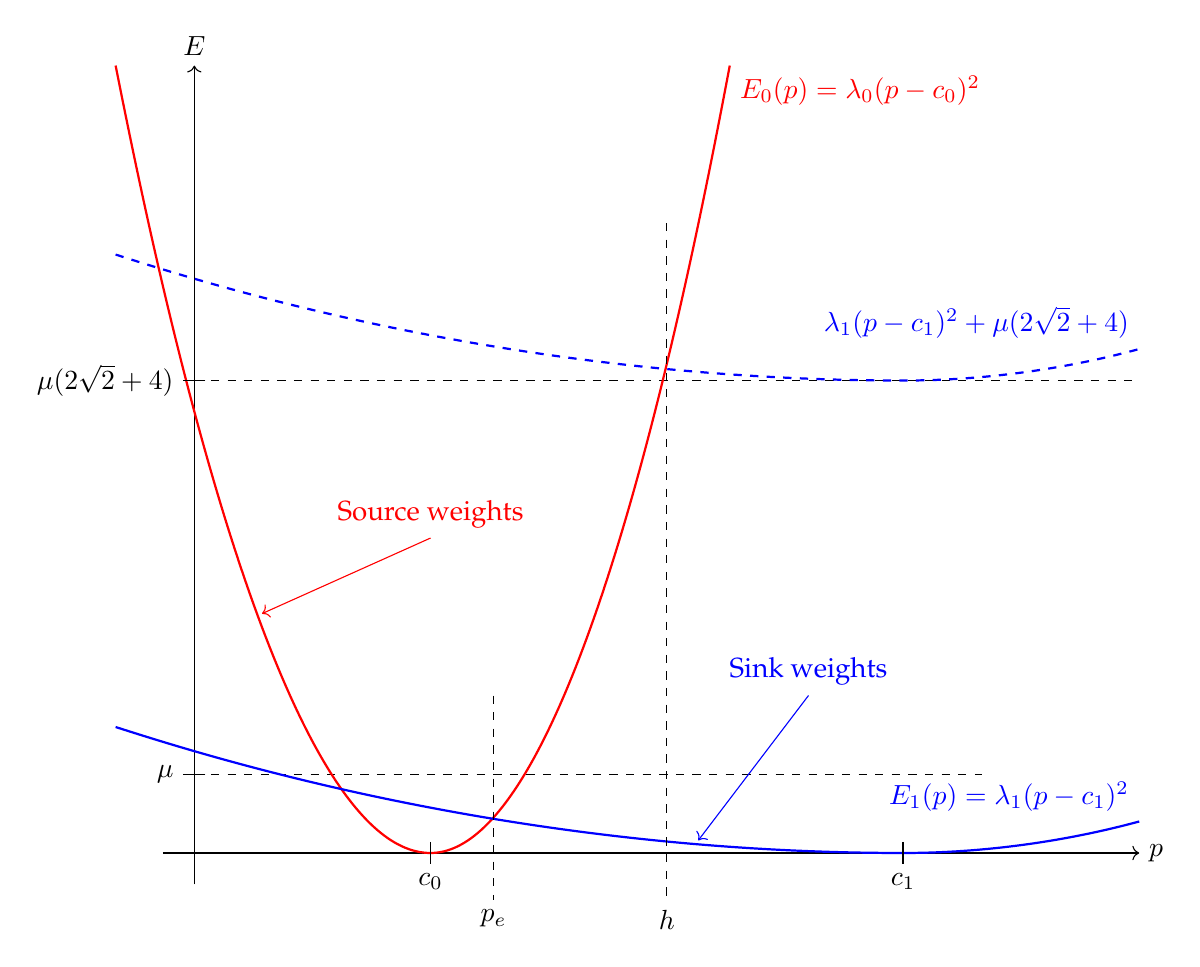
\begin{tikzpicture}[scale=2]
	\draw[->] (-0.2,0) -- (6,0) node[right] {$p$};
	\draw[->] (0,-0.2) -- (0,5) node[above] {$E$};
	
	\draw[dashed] (0,0.5) -- (5,0.5);
	\draw[dashed] (0,3) -- (6,3);
	\draw[red,thick] (-0.5,5) parabola bend (1.5,0) (3.4,5) node[below right] {$E_0(p) = \lambda_0 (p-c_0)^2$};
	\draw[blue,thick] (-0.5,0.8) parabola bend (4.5,0) (6,0.2) node[above left] {$E_1(p) = \lambda_1 (p-c_1)^2$};
	\draw[dashed,blue,thick] (-0.5,3.8) parabola bend (4.5,3) (6,3.2) node[above left] {$\lambda_1 (p-c_1)^2 + \mu(2\sqrt{2}+4)$};
	\draw[shift={(1.5,0)}] (0pt,2pt) -- (0pt,-2pt) node[below] {$c_0$};
	\draw[shift={(4.5,0)}] (0pt,2pt) -- (0pt,-2pt) node[below] {$c_1$};
	\draw[shift={(0,0.5)}] (2pt,0pt) -- (-2pt,0pt) node[left] {$\mu$};
	\draw[shift={(0,3)}] (2pt,0pt) -- (-2pt,0pt) node[left] {$\mu(2\sqrt{2}+4)$};
	
	\draw[dashed,black] (3.0,4) -- (3.0,-0.3) node[below] {$h$};
	\draw[dashed,black] (1.9,1) -- (1.9,-0.3) node[below] {$p_e$};
	%\draw[dashed,black] (0.94,1) -- (0.94,-0.3) node[below] {$p_e$};
	
	\draw[red,<-] (0.43,1.52) -- (1.5,2) node[above] {Source weights};
	\draw[blue,<-] (3.2,0.08) -- (3.9,1) node[above] {Sink weights};
	\end{tikzpicture}
	\caption{Data energy functions plot.}
	\label{fig:dataenergyplot}
\end{figure}

\begin{definition}[Analysis of the relationship between $p_e$ and $\alpha$]
	From \Cref{eq:pe} we note that there is one tunable parameter, i.e. $\alpha$. We can see that $p_e$ and $\alpha$ are inversely related. This is expressed mathematically as
\begin{equation*}\begin{split}
		\text{if } \alpha=1, p_e=c_0+\frac{c_1-c_0}{1+\sqrt{1}} = \frac{c_0+c_1}{2} \hspace{30pt}&\text{(midpoint between $c_0$ and $c_1$)}\\
		\lim_{\alpha\to\infty}p_e = \lim_{\alpha\to\infty}c_0+\frac{c_1-c_0}{1+\sqrt{\infty}} = c_0\hspace{30pt} &\text{(maximum $\alpha$ yields lowerbound on $p_e$)}\\
		\lim_{\alpha\to0}p_e = \lim_{\alpha\to0}c_0+\frac{c_1-c_0}{1+\sqrt{0}} = c_1\hspace{30pt} &\text{(minimum $\alpha$ yields upperbound on $p_e$)}
	\end{split}\end{equation*}
\end{definition}
The relationship between $p_e$ and $\alpha$ is illustrated in \Cref{fig:alphaperelationship}.
\begin{figure}[!h]
	\centering
	\begin{tikzpicture}[scale=1]
	\draw[->] (0,0) -- (15,0) node[right] {$p$};
	\draw[shift={(3,0)}] (0pt,4pt) -- (0pt,-4pt) node[below] {$c_0$};
	\draw[shift={(12,0)}] (0pt,4pt) -- (0pt,-4pt) node[below] {$c_1$};
	\draw[dashed,black] (7.5,1.5) node[above] {$p_e = \frac{c_0+c_1}{2}$} -- (7.5,-0.3) node[below] {$\alpha=1$};
	\draw[black,->,thick] (7.5,0.5) -- (5.5,0.5) node[above] {increasing $\alpha$} -- (4.5,0.5);
	\draw[black,->,thick] (7.5,0.5) -- (9.5,0.5) node[above] {decreasing $\alpha$} -- (10.5,0.5);
	\end{tikzpicture}
	\caption{Relationship between $\alpha$ and $p_e$.}
	\label{fig:alphaperelationship}
\end{figure}

\begin{definition}[Figuring $\alpha$]
	If we are able to make good estimates on $p_e$, $c_0$ and $c_1$ for the final segmented image, then it is possible to calculate $\alpha$ as follows:
	\begin{equation*}\begin{split}
		p_e &= c_0 + \frac{c_1-c_0}{\sqrt{\alpha} + 1} \\
		1+\sqrt{\alpha} &= \frac{c_1-c_0}{p_e-c_0}
		%\alpha &= \left( \frac{c_1-c_0}{p_e-c_0}-1 \right)^2
	\end{split}\end{equation*}
	\begin{equation}
		\alpha = \left( \frac{c_1-c_0}{p_e-c_0}-1 \right)^2
		\label{eq:alphaapproximation}
	\end{equation}
\end{definition}

\begin{definition}[Lowerbound on $\mu$]
	When we found the point, $p_e$, where the energies are equal in \Cref{eq:pe}, we ignored the other solution as it was not within the range from $c_0$ to $c_1$. Let this point be $p_{e^*}$. If this point is positive and $0<p_{e^*}<c_0$ then we must ensure that at no point within this range that the source flow saturates all the outgoing edges. This force a limit on how low $\mu$ can be. This is only of significant concern when $\alpha>1$. We only need to concern ourselve with the point $p=0$ as this is the point where the difference $E^i(0)-E^i(1)$ is the largest. The lowerbound on $\mu$ can be obtained as follows
	\begin{equation*}\begin{split}
		E^i(0)|_{p_i=0} &< E^i(1)|_{p_i=0} + \mu \left( 2\sqrt{2} + 4\right) \\
		\lambda_0c_0^2 &< \lambda_1c_1^2 + \mu \left( 2\sqrt{2} + 4\right) \\
		\therefore \mu \left( 2\sqrt{2} + 4\right) &> \lambda_0c_0^2 - \lambda_1c_1^2\\
		\mu &> \frac{\lambda_0c_0^2 - \lambda_1c_1^2}{\left( 2\sqrt{2} + 4\right)}
	\end{split}\end{equation*} 
\end{definition}
Taking into account the relation in \Cref{eq:l0l1dependancy} this becomes
\begin{equation}
	\mu > \frac{\lambda_1(\alpha c_0^2-c_1^2)}{\left( 2\sqrt{2} + 4\right)}
	\label{eq:mulowerbound}
\end{equation}

\begin{definition}[Absolutely in the source set] From \Cref{eq:sourcesaturation} we can see that there is a point beyond which all nodes which correspond to pixel value higher than that point will be saturated and have excess flow which means that they will be in the source set. We will call this point the \textit{saturation point} and denote it by $h$. This is shown in \Cref{fig:dataenergyplot}. This point can be determined as follows:
\begin{equation*}\begin{split}
	\lambda_0(h-c_0)^2 &> \lambda_1(h-c_1)^2 + f_{max} \\
	\lambda_0(h-c_0)^2 - \lambda_1(h-c_1)^2 &> f_{max} \\
	(\lambda_0-\lambda_1)h^2 + (-2\lambda_0 c_0 + 2\lambda_1 c_1)h + (\lambda_0 c_0^2 - \lambda_1 c_1^2-f_{max}) &> 0
\end{split}\end{equation*}
The solutions to $h$ are
\begin{equation*}\begin{split}
	h = \frac{ (2\lambda_0 c_0 - 2\lambda_1 c_1) \pm \sqrt{(-2\lambda_0 c_0 + 2\lambda_1 c_1)^2-4(\lambda_0-\lambda_1)(\lambda_0 c_0^2 - \lambda_1 c_1^2-f_{max})}}{2(\lambda_0-\lambda_1)}
\end{split}\end{equation*}
Substituting the relation in \Cref{eq:l0l1dependancy}
\begin{equation*}\begin{split}
	h &= \frac{(\alpha c_0-c_1)\pm\sqrt{(c_1-\alpha c_0)^2-(\alpha-1)(\alpha c_0^2-c_1^2-\frac{f_{max}}{\lambda_1})}}{\alpha-1}\\
	&= \frac{(\alpha c_0-c_1)\pm\sqrt{\alpha(c_0-c_1)^2+\frac{f_{max}}{\lambda_1}(\alpha-1)}}{\alpha-1}
\end{split}\end{equation*}
If the $\mu$ is greater than the lowerbound in \Cref{eq:mulowerbound} then there is only one solution to $h$ which is of importance. This is the positive solution for $h$ which is
\begin{equation}
	h = \frac{(\alpha c_0-c_1)+\sqrt{\alpha(c_0-c_1)^2+\frac{\mu(2\sqrt{2}+4)}{\lambda_1}(\alpha-1)}}{\alpha-1}
	\label{eq:h}
\end{equation}
This point is marked off in \Cref{fig:dataenergyplot}.
\end{definition}

\begin{definition}[Determining $\lambda_1$] Given good approximations for $c_0$, $c_1$, $\alpha$, $h$ and $\mu$, we can calculate the appropriate value for $\lambda_1$. We proceed from \Cref{eq:sourcesaturation} as follows
\begin{equation*}\begin{split}
	\lambda_0(h-c_0)^2 &= \lambda_1(h-c_1)^2 + \mu(2\sqrt{2}+4)\\
	\lambda_1 \left( \alpha(h-c_0)^2-(h-c_1)^2 \right) &= \mu(2\sqrt{2}+4)
\end{split}\end{equation*}
\begin{equation}
	\lambda_1 = \frac{\mu(2\sqrt{2}+4)}{\alpha(h-c_0)^2-(h-c_1)^2}
	\label{eq:lambda1approximation}
\end{equation}
\end{definition}

\begin{definition}[Parameter estimation process]
	The parameter estimation is based on the assumption that sufficiently good approximations for $c_0$, $c_1$, $p_e$ and $h$ can be obtained. By sufficiently good we are referring to the closeness to the values these parameters would take for an ideal segmetation. From these approximations, we calculate the approximation for $\alpha$ using \Cref{eq:alphaapproximation}. The parameters $\mu$ and $\lambda_1$ are related and aren't seperable, therefore we set choose to set $\mu$. We can then calculate $\lambda_1$ using \Cref{eq:lambda1approximation}. For the chosen $\mu$ we can calculate the upperbound on $\lambda_1$ to ensure that the constraint \Cref{eq:mulowerbound} is met. The constraint on $\lambda_1$ is calculated as follows
\begin{equation*}
\mu\left( 2\sqrt{2} + 4 \right) > \lambda_1(\alpha c_0^2 - c_1^2)
\end{equation*}
\begin{equation}
	\lambda_1 < \frac{\mu\left( 2\sqrt{2} + 4 \right)}{\alpha c_0^2 - c_1^2}
\end{equation}
Finally $\lambda_0$ can be calculated using \Cref{eq:l0l1dependancy}.
\end{definition}

\subsection{Tuning Parameters for Fluorescence Microscopy}
\label{sec:cvgc_parameterestimation}

%\textcolor{red}{What sort of image properties are we tuning for? E.g. dark bg, low contrast, etc. Parameters limits and ranges.}
The properties of the images obtained in fluorescence microscopy imaging can be used to guide the parameter estimation process. We focus, specifically, on black background images. Due to the fact that the predominant form of noise in the imaging system in Poisson distributed, we can further assume that the darker the background, the less noise that is present therein. The Poisson process also tells us that brighter regions exhibit a greater intensity variation due to the sampling process. Therefore, the curve for $E^i(1)$ is less convex than $E^i(0)$ as in \Cref{fig:dataenergyplot} and, resultantly, the value for $p_e$, in \Cref{fig:alphaperelationship}, is shifted to the left. This places a new lowerbound on $\alpha$ for fluorescence images
\begin{equation}
	\alpha \geq 1.
	\label{eq:alphalowerboundFM}
\end{equation}

\begin{definition}[Manual Tuning] Before moving further into analysis of the relationships between the parameters, we first peform a manual tuning of parameters and observing the effect on the segmented results. This allows us to understand how strongly correlated the parameter is to the final result. We note that the curves, $E^i(0)$ and $E^i(1)$, can be tuned relative to a fixed value for $\mu$ and this wouldn't impact significantly on the range of possible solution sets. Therefore, we set $\mu=1$ in all our manual parameter tuning. We use a stopping criterion of $\epsilon=1\times10^{-3}$.
	
We cover a relatively wide range of parameter settings and note the output, i.e. over-segmented, under-segmented, almost ideal, etc. At this point, catergorising the segemented output is largely subjective. We also use various initial conditions. Specifically, we use the segmented output from Otsu binarization, K-means ($k=2$) and Expectation-Maximisation for Gaussian Mixture Modelling (EMGMM) with ($k=2$). The initial and final means are of significant important in this study.

For \Cref{fig:1gray}, we used show the output for the following combinations of $\alpha$ and $\lambda_1$. $(\alpha,\lambda_1) = \{(30,150), (40,50), (40,100), (40,150), (40,200), (45,150), (50,150)\}$. The initial segmentation masks are shown in \Cref{fig:image1init}. The segmented output for the combinations are shown in \Cref{fig:image1mytune}.

For \Cref{fig:2gray}, we used show the output for the following combinations of $\alpha$ and $\lambda_1$. $(\alpha,\lambda_1) = \{(30,150), (40,50), (40,100), (40,150), (40,200), (45,150), (50,150)\}$. The initial segmentation masks are shown in \Cref{fig:image2init}. The segmented output for the combinations are shown in \Cref{fig:image2mytune}.

For \Cref{fig:3gray}, we used show the output for the following combinations of $\alpha$ and $\lambda_1$. $(\alpha,\lambda_1) = \{(1,150), (10,150), (10,200), (10,400), (10,800), (20,150), (30,150), (40,150), (50,150)\}$. The initial segmentation masks are shown in \Cref{fig:image3init}. The segmented output for the combinations are shown in \Cref{fig:image3mytune}.

For \Cref{fig:4gray}, we used show the output for the following combinations of $\alpha$ and $\lambda_1$. $(\alpha,\lambda_1) = \{(30,50), (30,100), (30,150), (40,100), (40,150), (50,150)\}$. The initial segmentation masks are shown in \Cref{fig:image4init}. The segmented output for the combinations are shown in \Cref{fig:image4mytune}.

For \Cref{fig:5gray}, we used show the output for the following combinations of $\alpha$ and $\lambda_1$. $(\alpha,\lambda_1) = \{(30,50), (30,100), (30,150), (40,100), (40,150), (50,150)\}$. The initial segmentation masks are shown in \Cref{fig:image5init}. The segmented output for the combinations are shown in \Cref{fig:image5mytune}.

For \Cref{fig:6gray}, we used show the output for the following combinations of $\alpha$ and $\lambda_1$. $(\alpha,\lambda_1) = \{(20,20), (20,150), (30,150), (40,50), (40,150), (50,150)\}$. The initial segmentation masks are shown in \Cref{fig:image6init}. The segmented output for the combinations are shown in \Cref{fig:image6mytune}.

The means and standard deviations for the initial masks obtained are shown in \Cref{tab:initmaskvalues}.

\clearpage

\begin{figure}[!t]
	\centering
	\subfigure[Otsu]
	{
		\includegraphics[width=0.3\columnwidth]{mymanualtuning/image1/otsu_init.jpg}
		\label{fig:1grayotsu}
	}
	\subfigure[K-Means ($k=2$)]
	{
		\includegraphics[width=0.3\columnwidth]{mymanualtuning/image1/kmeans_init.jpg}
		\label{fig:1graykmeans}
	}
	\subfigure[EMGMM ($k=2$)]
	{
		\includegraphics[width=0.3\columnwidth]{mymanualtuning/image1/emgmm_init.jpg}
		\label{fig:1grayemgmm}
	}
	\caption{Image 1 from sample set \Cref{fig:sampleset} initial masks.}
	\label{fig:image1init}
\end{figure}

\begin{figure}[!t]
	\centering
	\subfigure[$\mu=1$, $\alpha=30$, $\lambda_1=150$]
	{
		\includegraphics[width=0.3\columnwidth]{mymanualtuning/image1/1_30_150.jpg}
		\label{fig:1graymytune1}
	}
	\subfigure[$\mu=1$, $\alpha=40$, $\lambda_1=50$]
	{
		\includegraphics[width=0.3\columnwidth]{mymanualtuning/image1/1_40_50.jpg}
		\label{fig:1graymytune2}
	}
	\subfigure[$\mu=1$, $\alpha=40$, $\lambda_1=100$]
	{
		\includegraphics[width=0.3\columnwidth]{mymanualtuning/image1/1_40_100.jpg}
		\label{fig:1graymytune3}
	}
	\subfigure[$\mu=1$, $\alpha=40$, $\lambda_1=150$]
	{
		\includegraphics[width=0.3\columnwidth]{mymanualtuning/image1/1_40_150.jpg}
		\label{fig:1graymytune4}
	}
	\subfigure[$\mu=1$, $\alpha=40$, $\lambda_1=200$]
	{
		\includegraphics[width=0.3\columnwidth]{mymanualtuning/image1/1_40_200.jpg}
		\label{fig:1graymytune5}
	}
%	\subfigure[$\mu=1$, $\alpha=45$, $\lambda_1=150$]
%	{
%		\includegraphics[width=0.3\columnwidth]{mymanualtuning/image1/1_45_150.jpg}
%		\label{fig:1graymytune6}
%	}
	\subfigure[$\mu=1$, $\alpha=50$, $\lambda_1=150$]
	{
		\includegraphics[width=0.3\columnwidth]{mymanualtuning/image1/1_50_150.jpg}
		\label{fig:1graymytune7}
	}
	\caption{Segmented output for various combination of $\alpha$ and $\lambda_1$ for Image 1 in the sample set.}
	\label{fig:image1mytune}
\end{figure}

\begin{figure}[!t]
	\centering
	\subfigure[Otsu]
	{
		\includegraphics[width=0.3\columnwidth]{mymanualtuning/image2/otsu_init.jpg}
		\label{fig:2grayotsu}
	}
	\subfigure[K-Means ($k=2$)]
	{
		\includegraphics[width=0.3\columnwidth]{mymanualtuning/image2/kmeans_init.jpg}
		\label{fig:2graykmeans}
	}
	\subfigure[EMGMM ($k=2$)]
	{
		\includegraphics[width=0.3\columnwidth]{mymanualtuning/image2/emgmm_init.jpg}
		\label{fig:2grayemgmm}
	}
	\caption{Image 2 from sample set \Cref{fig:sampleset} initial masks.}
	\label{fig:image2init}
\end{figure}

\begin{figure}[!t]
	\centering
	\subfigure[$\mu=1$, $\alpha=30$, $\lambda_1=150$]
	{
		\includegraphics[width=0.3\columnwidth]{mymanualtuning/image2/1_30_150.jpg}
		\label{fig:2graymytune1}
	}
	\subfigure[$\mu=1$, $\alpha=40$, $\lambda_1=50$]
	{
		\includegraphics[width=0.3\columnwidth]{mymanualtuning/image2/1_40_50.jpg}
		\label{fig:2graymytune2}
	}
%	\subfigure[$\mu=1$, $\alpha=40$, $\lambda_1=100$]
%	{
%		\includegraphics[width=0.3\columnwidth]{mymanualtuning/image2/1_40_100.jpg}
%		\label{fig:2graymytune3}
%	}
	\subfigure[$\mu=1$, $\alpha=40$, $\lambda_1=150$]
	{
		\includegraphics[width=0.3\columnwidth]{mymanualtuning/image2/1_40_150.jpg}
		\label{fig:2graymytune4}
	}
	\subfigure[$\mu=1$, $\alpha=40$, $\lambda_1=200$]
	{
		\includegraphics[width=0.3\columnwidth]{mymanualtuning/image2/1_40_200.jpg}
		\label{fig:2graymytune5}
	}
	\subfigure[$\mu=1$, $\alpha=45$, $\lambda_1=150$]
	{
		\includegraphics[width=0.3\columnwidth]{mymanualtuning/image2/1_45_150.jpg}
		\label{fig:2graymytune6}
	}
	\subfigure[$\mu=1$, $\alpha=50$, $\lambda_1=150$]
	{
		\includegraphics[width=0.3\columnwidth]{mymanualtuning/image2/1_50_150.jpg}
		\label{fig:2graymytune7}
	}
	\caption{Segmented output for various combination of $\alpha$ and $\lambda_1$ for Image 2 in the sample set.}
	\label{fig:image2mytune}
\end{figure}

\begin{figure}[!t]
	\centering
	\subfigure[Otsu]
	{
		\includegraphics[width=0.3\columnwidth]{mymanualtuning/image3/otsu_init.jpg}
		\label{fig:3grayotsu}
	}
	\subfigure[K-means ($k=2$)]
	{
		\includegraphics[width=0.3\columnwidth]{mymanualtuning/image3/kmeans_init.jpg}
		\label{fig:3graykmeans}
	}
	\subfigure[EMGMM ($k=2$)]
	{
		\includegraphics[width=0.3\columnwidth]{mymanualtuning/image3/emgmm_init.jpg}
		\label{fig:3grayemgmm}
	}
	\caption{Image 3 from sample set \Cref{fig:sampleset} initial masks.}
	\label{fig:image3init}
\end{figure}

\begin{figure}[!t]
	\centering
	\subfigure[$\mu=1$, $\alpha=1$, $\lambda_1=150$]
	{
		\includegraphics[width=0.3\columnwidth]{mymanualtuning/image3/1_1_150.jpg}
		\label{fig:3graymytune1}
	}
%	\subfigure[$\mu=1$, $\alpha=10$, $\lambda_1=150$]
%	{
%		\includegraphics[width=0.3\columnwidth]{mymanualtuning/image3/1_10_150.jpg}
%		\label{fig:3graymytune2}
%	}
%	\subfigure[$\mu=1$, $\alpha=10$, $\lambda_1=200$]
%	{
%		\includegraphics[width=0.3\columnwidth]{mymanualtuning/image3/1_10_200.jpg}
%		\label{fig:3graymytune3}
%	}
	\subfigure[$\mu=1$, $\alpha=10$, $\lambda_1=400$]
	{
		\includegraphics[width=0.3\columnwidth]{mymanualtuning/image3/1_10_400.jpg}
		\label{fig:3graymytune4}
	}
	\subfigure[$\mu=1$, $\alpha=10$, $\lambda_1=800$]
	{
		\includegraphics[width=0.3\columnwidth]{mymanualtuning/image3/1_10_800.jpg}
		\label{fig:3graymytune5}
	}
	\subfigure[$\mu=1$, $\alpha=20$, $\lambda_1=150$]
	{
		\includegraphics[width=0.3\columnwidth]{mymanualtuning/image3/1_20_150.jpg}
		\label{fig:3graymytune6}
	}
	\subfigure[$\mu=1$, $\alpha=30$, $\lambda_1=150$]
	{
		\includegraphics[width=0.3\columnwidth]{mymanualtuning/image3/1_30_150.jpg}
		\label{fig:3graymytune7}
	}
	\subfigure[$\mu=1$, $\alpha=40$, $\lambda_1=150$]
	{
		\includegraphics[width=0.3\columnwidth]{mymanualtuning/image3/1_40_150.jpg}
		\label{fig:3graymytune8}
	}
%	\subfigure[$\mu=1$, $\alpha=50$, $\lambda_1=150$]
%	{
%		\includegraphics[width=0.3\columnwidth]{mymanualtuning/image3/1_50_150.jpg}
%		\label{fig:3graymytune9}
%	}
	\caption{Segmented output for various combination of $\alpha$ and $\lambda_1$ for Image 3 in the sample set.}
	\label{fig:image3mytune}
\end{figure}

\begin{figure}[!t]
	\centering
	\subfigure[Otsu]
	{
		\includegraphics[width=0.3\columnwidth]{mymanualtuning/image4/otsu_init.jpg}
		\label{fig:4grayotsu}
	}
	\subfigure[K-means ($k=2$)]
	{
		\includegraphics[width=0.3\columnwidth]{mymanualtuning/image4/kmeans_init.jpg}
		\label{fig:4graykmeans}
	}
	\subfigure[EMGMM ($k=2$)]
	{
		\includegraphics[width=0.3\columnwidth]{mymanualtuning/image4/emgmm_init.jpg}
		\label{fig:4grayemgmm}
	}
	\caption{Image 4 from sample set \Cref{fig:sampleset} initial masks.}
	\label{fig:image4init}
\end{figure}

\begin{figure}[!t]
	\centering
	\subfigure[$\mu=1$, $\alpha=30$, $\lambda_1=50$]
	{
		\includegraphics[width=0.3\columnwidth]{mymanualtuning/image4/1_30_50.jpg}
		\label{fig:4graymytune1}
	}
	\subfigure[$\mu=1$, $\alpha=30$, $\lambda_1=100$]
	{
		\includegraphics[width=0.3\columnwidth]{mymanualtuning/image4/1_30_100.jpg}
		\label{fig:4graymytune2}
	}
	\subfigure[$\mu=1$, $\alpha=30$, $\lambda_1=150$]
	{
		\includegraphics[width=0.3\columnwidth]{mymanualtuning/image4/1_30_150.jpg}
		\label{fig:4graymytune3}
	}
	\subfigure[$\mu=1$, $\alpha=40$, $\lambda_1=100$]
	{
		\includegraphics[width=0.3\columnwidth]{mymanualtuning/image4/1_40_100.jpg}
		\label{fig:4graymytune4}
	}
	\subfigure[$\mu=1$, $\alpha=40$, $\lambda_1=150$]
	{
		\includegraphics[width=0.3\columnwidth]{mymanualtuning/image4/1_40_150.jpg}
		\label{fig:4graymytune5}
	}
	\subfigure[$\mu=1$, $\alpha=50$, $\lambda_1=150$]
	{
		\includegraphics[width=0.3\columnwidth]{mymanualtuning/image4/1_50_150.jpg}
		\label{fig:4graymytune6}
	}
	\caption{Segmented output for various combination of $\alpha$ and $\lambda_1$ for Image 4 in the sample set.}
	\label{fig:image4mytune}
\end{figure}

\begin{figure}[!t]
	\centering
	\subfigure[Otsu]
	{
		\includegraphics[width=0.3\columnwidth]{mymanualtuning/image5/otsu_init.jpg}
		\label{fig:5grayotsu}
	}
	\subfigure[K-means ($k=2$)]
	{
		\includegraphics[width=0.3\columnwidth]{mymanualtuning/image5/kmeans_init.jpg}
		\label{fig:5graykmeans}
	}
	\subfigure[EMGMM ($k=2$)]
	{
		\includegraphics[width=0.3\columnwidth]{mymanualtuning/image5/emgmm_init.jpg}
		\label{fig:5grayemgmm}
	}
	\caption{Image 5 from sample set \Cref{fig:sampleset} initial masks.}
	\label{fig:image5init}
\end{figure}

\begin{figure}[!t]
	\centering
	\subfigure[$\mu=1$, $\alpha=30$, $\lambda_1=50$]
	{
		\includegraphics[width=0.3\columnwidth]{mymanualtuning/image5/1_30_50.jpg}
		\label{fig:5graymytune1}
	}
	\subfigure[$\mu=1$, $\alpha=30$, $\lambda_1=100$]
	{
		\includegraphics[width=0.3\columnwidth]{mymanualtuning/image5/1_30_100.jpg}
		\label{fig:5graymytune2}
	}
	\subfigure[$\mu=1$, $\alpha=30$, $\lambda_1=150$]
	{
		\includegraphics[width=0.3\columnwidth]{mymanualtuning/image5/1_30_150.jpg}
		\label{fig:5graymytune3}
	}
	\subfigure[$\mu=1$, $\alpha=40$, $\lambda_1=150$]
	{
		\includegraphics[width=0.3\columnwidth]{mymanualtuning/image5/1_40_100.png}
		\label{fig:5graymytune4}
	}
	\subfigure[$\mu=1$, $\alpha=40$, $\lambda_1=150$]
	{
		\includegraphics[width=0.3\columnwidth]{mymanualtuning/image5/1_40_150.jpg}
		\label{fig:5graymytune5}
	}
	\subfigure[$\mu=1$, $\alpha=50$, $\lambda_1=150$]
	{
		\includegraphics[width=0.3\columnwidth]{mymanualtuning/image5/1_50_150.jpg}
		\label{fig:5graymytune6}
	}
	\caption{Segmented output for various combination of $\alpha$ and $\lambda_1$ for Image 5 in the sample set.}
	\label{fig:image5mytune}
\end{figure}

\begin{figure}[!t]
	\centering
	\subfigure[Otsu]
	{
		\includegraphics[width=0.3\columnwidth]{mymanualtuning/image6/otsu_init.jpg}
		\label{fig:6grayotsu}
	}
	\subfigure[K-means ($k=2$)]
	{
		\includegraphics[width=0.3\columnwidth]{mymanualtuning/image6/kmeans_init.jpg}
		\label{fig:6graykmeans}
	}
	\subfigure[EMGMM ($k=2$)]
	{
		\includegraphics[width=0.3\columnwidth]{mymanualtuning/image6/emgmm_init.jpg}
		\label{fig:6grayemgmm}
	}
	\caption{Image 6 from sample set \Cref{fig:sampleset} initial masks.}
	\label{fig:image6init}
\end{figure}

\begin{figure}[!t]
	\centering
	\subfigure[$\mu=1$, $\alpha=20$, $\lambda_1=20$]
	{
		\includegraphics[width=0.3\columnwidth]{mymanualtuning/image6/1_20_20.jpg}
		\label{fig:6graymytune1}
	}
%	\subfigure[$\mu=1$, $\alpha=20$, $\lambda_1=50$]
%	{
%		\includegraphics[width=0.3\columnwidth]{mymanualtuning/image6/1_20_50.jpg}
%		\label{fig:6graymytune2}
%	}
	\subfigure[$\mu=1$, $\alpha=20$, $\lambda_1=150$]
	{
		\includegraphics[width=0.3\columnwidth]{mymanualtuning/image6/1_20_150.jpg}
		\label{fig:6graymytune2}
	}
	\subfigure[$\mu=1$, $\alpha=30$, $\lambda_1=150$]
	{
		\includegraphics[width=0.3\columnwidth]{mymanualtuning/image6/1_30_150.jpg}
		\label{fig:6graymytune3}
	}
	\subfigure[$\mu=1$, $\alpha=40$, $\lambda_1=50$]
	{
		\includegraphics[width=0.3\columnwidth]{mymanualtuning/image6/1_40_50.jpg}
		\label{fig:6graymytune4}
	}
	\subfigure[$\mu=1$, $\alpha=40$, $\lambda_1=150$]
	{
		\includegraphics[width=0.3\columnwidth]{mymanualtuning/image6/1_40_150.jpg}
		\label{fig:6graymytune5}
	}
	\subfigure[$\mu=1$, $\alpha=50$, $\lambda_1=150$]
	{
		\includegraphics[width=0.3\columnwidth]{mymanualtuning/image6/1_50_150.jpg}
		\label{fig:6graymytune6}
	}
	\caption{Segmented output for various combination of $\alpha$ and $\lambda_1$ for Image 6 in the sample set.}
	\label{fig:image6mytune}
\end{figure}

\end{definition}

\clearpage

\begin{table}[t!]
	\centering
	\caption{Initial means and standard deviations for all images in the sample set for Otsu, K-means and EMGMM clustering.}
	\begin{tabular}{|c|c|c|c|c|}
	\hline
	& $c_0$ & $c_1$ & $s_0$ & $s_1$\\
	\hline
	Image 1 & & & & \\
	\hline
	Otsu & $0.0307515$ & $0.26466$ & $0.0385001$ & $0,0803506$ \\
	\hline
	K-means($k=2$) & $0.0308984$ & $0.267192$ & $0.0387009$ & $0.0793621$ \\
	\hline
	EMGMM ($k=2$) & $0.0305648$ & $0.261392$ & $0.0382529$ & $0.081608$ \\
	\hline
	Image 2 & & & & \\
	\hline
	Otsu & $0.0293218$ & $0.373293$ & $0.054652$ & $0.124376$ \\
	\hline
	K-means($k=2$) & $0.0293218$ & $0.373293$ & $0.054652$ & $0.124376$ \\
	\hline
	EMGMM ($k=2$) & $0.010789$ & $0.321058$ & $0.0211362$ & $0.140498$ \\
	\hline
	Image 3 & & & & \\
	\hline
	Otsu & $0.0422978$ & $0.105043$ & $0.0104066$ & $0.0269333$ \\
	\hline
	K-means($k=2$) & $0.0422978$ & $0.105043$ & $0.0104066$ & $0.0269333$ \\
	\hline
	EMGMM ($k=2$) & $0.042026$ & $0.103124$ & $0.0100784$ & $0.0273395$ \\
	\hline
	Image 4 & & & & \\
	\hline
	Otsu & $0.0424602$ & $0.147303$ & $0.0133024$ & $0.0513289$ \\
	\hline
	K-means($k=2$) & $0.0420671$ & $0.145145$ & $0.0125633$ & $0.0513602$ \\
	\hline
	EMGMM ($k=2$) & $0.0407566$ & $0.136167$ & $0.0102742$ & $0.052472$ \\
	\hline
	Image 5 & & & & \\
	\hline
	Otsu & $0.037086$ & $0.216513$ & $0.0138978$ & $0.0626164$ \\
	\hline
	K-means($k=2$) & $-$ & $-$ & $-$ & $-$ \\
	\hline
	EMGMM ($k=2$) & $0.0343141$ & $0.190501$ & $0.00456055$ & $0.0782783$ \\
	\hline
	Image 6 & & & & \\
	\hline
	Otsu & $0.270483$ & $0.00657006$ & $0.0228327$ & $0.0916426$ \\
	\hline
	K-means($k=2$) & $0.270483$ & $0.00657006$ & $0.0228327$ & $0.0916426$ \\
	\hline
	EMGMM ($k=2$) & $0$ & $0.187883$ & $0$ & $0.133022$ \\
	\hline
\end{tabular}
\label{tab:initmaskvalues}
\end{table}

The final values for the segmentation results are shown in \Cref{tab:manualresults}. The table shows for each image, given the values for the input parameters, whether the degree of acceptance of the output. We take the  final results are the means of object and the background. From the final results, we calculate the values for $p_e$, \Cref{eq:pe}, and $h$ ,\Cref{eq:h}. The means for each image can vary greatly. To put the values of $p_e$ and $h$ into a relative perspective, they are also shown as a fraction of the distance between $c_0$ and $c_1$. Let $k_p \in (0,1)$ be the fraction of the distance $p_e-c_0$ and $c_1-c_0$ as illustrated in \Cref{fig:kp}. Let $k_h \in (k_h,1)$ be the fraction of the distance $h-c_0$ and $c_1-c_0$ as illustrated in \Cref{fig:kh}. The following relation holds $0 < k_p < k_h$.

\begin{figure}[!h]
	\centering
	\begin{tikzpicture}[scale=1]
	\draw[-] (0,0) -- (15,0) node[right] {$p$};
	\draw[shift={(3,0)}] (0pt,4pt) -- (0pt,-4pt) node[below] {$c_0$};
	\draw[shift={(12,0)}] (0pt,4pt) -- (0pt,-4pt) node[below] {$c_1$};
	
	\draw[dashed,black] (5.0,1.5) -- (5.0,-0.3) node[below] {$p_e$};
	
	\draw[black,*-*,thick] (5.0,0.5) -- (4.0,0.5) node[above] {$k_p(c_1-c_0)$} -- (3.0,0.5);
	
	\end{tikzpicture}
	\caption{$p_e$ as a fraction of the distance between $c_0$ and $c_1$.}
	\label{fig:kp}
\end{figure}

\begin{figure}[!h]
	\centering
	\begin{tikzpicture}[scale=1]
	\draw[-] (0,0) -- (15,0) node[right] {$p$};
	\draw[shift={(3,0)}] (0pt,4pt) -- (0pt,-4pt) node[below] {$c_0$};
	\draw[shift={(12,0)}] (0pt,4pt) -- (0pt,-4pt) node[below] {$c_1$};
	
	\draw[dashed,black] (9.0,1.5) -- (9.0,-0.3) node[below] {$h$};
	
	\draw[black,*-*,thick] (9.0,0.5) -- (6.0,0.5) node[above] {$k_h(c_1-c_0)$} -- (3.0,0.5);
	\draw[black,*-*,thick] (9.0,0.5) -- (10.5,0.5) node[above] {$(1-k_h)(c_1-c_0)$} -- (12.0,0.5);
	\end{tikzpicture}
	\caption{$h$ as a fraction of the distance between $c_0$ and $c_1$.}
	\label{fig:kh}
\end{figure}

\begin{center}
	\begin{longtable}{|c|c|c|c|c|c|c|c|c|}
	\caption{Results from manual tuning.} \label{tab:manualresults}\\
	\hline 
	Image & $\alpha$ & $\lambda_1$ & $c_0$ & $c_1$ & $p_e$ & $h$ & $k_p$ & $k_h$ \\ 	
	\hline \rowcolor{bad} 1-O &	30 &	100 &	0.009171 &	0.117209 &	0.025851 &	0.058086 &	0.154387 &	0.452755 \\
	\hline 1-O &	40 &	100	&	0.006909 &	0.110953 &	0.021114 &	0.049359 &	0.136527 &	0.407996 \\
	\hline 1-O &	40 &	50	&	0.006803 &	0.110618 &	0.020976 &	0.065665 &	0.136527 &	0.566987 \\
	\hline \rowcolor{acceptable} 1-O &	40 & 	150	&	0.006953 &	0.111119 &	0.021175 &	0.042396 &	0.136527 &	0.340248 \\
	\hline \rowcolor{acceptable} 1-O &	40 &	200 &	0.007093 &	0.111541 &	0.021353 &	0.038508 &	0.136527 &	0.300772 \\
	\hline \rowcolor{acceptable} 1-O &	45 &	150 &	0.006832 &	0.110758 &	0.020314 &	0.040326 &	0.129732 &	0.322287 \\
	\hline \rowcolor{acceptable} 1-O &	50 &	150 &	0.006681 &	0.110301 &	0.019519 &	0.038516 &	0.123899 &	0.307235 \\
	\hline \rowcolor{bad} 1-K &	30 &	100 &	0.009557 &	0.118306 &	0.026346 &	0.058499 &	0.154387 &	0.450049 \\
	\hline \rowcolor{acceptable} 1-K &	40 &	100 &	0.006928 &	0.111013 &	0.021138 &	0.049379 &	0.136527 &	0.407847 \\
	\hline 1-K &	40 &	50  &	0.006818 &	0.110658 &	0.020995 &	0.065680 &	0.136527 &	0.566856 \\
	\hline \rowcolor{acceptable} 1-K &	40 &	150 &	0.007063 &	0.111430 &	0.021312 &	0.042514 &	0.136527 &	0.339679 \\
	\hline \rowcolor{acceptable} 1-K &	40 &	200 &	0.007176 &	0.111789 &	0.021459 &	0.038600 &	0.136527 &	0.300384 \\
	\hline \rowcolor{acceptable} 1-K &	45 &	150 &	0.006852 &	0.110824 &	0.020340 &	0.040348 &	0.129732 &	0.322165 \\
	\hline \rowcolor{acceptable} 1-K &	50 &	150 &	0.006685 &	0.110311 &	0.019524 &	0.038521 &	0.123899 &	0.307219 \\
	\hline \rowcolor{bad} 1-E &	30 &	150 &	0.008876 &	0.116478 &	0.025489 &	0.049694 &	0.154387 &	0.379343 \\
	\hline \rowcolor{acceptable} 1-E &	40 &	100 &	0.006687 &	0.110890 &	0.020913 &	0.049142 &	0.136527 &	0.407426 \\
	\hline 1-E &	40 &	50  &	0.006788 &	0.110583 &	0.020959 &	0.065649 &	0.136527 &	0.567093 \\
	\hline \rowcolor{acceptable} 1-E &	40 &	150 &	0.006944 &	0.111087 &	0.021163 &	0.042385 &	0.136527 &	0.340313 \\
	\hline \rowcolor{acceptable} 1-E &	40 &	200 &	0.007058 &	0.111434 &	0.021308 &	0.038469 &	0.136527 &	0.300940 \\
	\hline 1-E &	45 &	150 &	0.006800 &	0.110654 &	0.020273 &	0.040291 &	0.129732 &	0.322481 \\
	\hline \rowcolor{acceptable} 1-E &	50 &	150 &	0.006676 &	0.110283 &	0.019512 &	0.038510 &	0.123899 &	0.307268 \\	
	\hline 2-O &	30 &	150 &	0.007640 &	0.309246 &	0.054204 &	0.066628 &	0.154387 &	0.195579 \\
	\hline 2-O &	40 &	50	&	0.007449 &	0.308057 &	0.048489 &	0.076410 &	0.136527 &	0.229407 \\
	\hline 2-O &	40 &	100	&	0.007428 &	0.307890 &	0.048449 &	0.063950 &	0.136527 &	0.188118 \\
	\hline 2-O &	40 &	150	& 	0.007424 &	0.307975 &	0.048457 &	0.059239 &	0.136527 &	0.172400 \\
	\hline 2-O &	40 &	200	&	0.007441 &	0.308094 &	0.048488 &	0.056764 &	0.136527 &	0.164052 \\
	\hline 2-O &	45 &	150	&	0.007423 &	0.307976 &	0.046415 &	0.056577 &	0.129732 &	0.163545 \\
	\hline 2-O &	50 &	150	&	0.007297 &	0.307166 &	0.044450 &	0.054107 &	0.123899 &	0.156103 \\
	\hline 2-K &	30 &	150	&	0.007640 &	0.309246 &	0.054204 &	0.066628 &	0.154387 &	0.195579 \\
	\hline 2-K &	40 &	50	&	0.007449 &	0.308057 &	0.048489 &	0.076410 &	0.136527 &	0.229407 \\
	\hline 2-K &	40 &	100	&	0.007428 &	0.307890 &	0.048449 &	0.063950 &	0.136527 &	0.188118 \\
	\hline 2-K &	40 &	150	&	0.007424 &	0.307975 &	0.048457 &	0.059239 &	0.136527 &	0.172400 \\
	\hline 2-K &	40 &	200	&	0.007441 &	0.308094 &	0.048488 &	0.056764 &	0.136527 &	0.164052 \\
	\hline 2-K &	45 &	150	&	0.007423 &	0.307976 &	0.046415 &	0.056577 &	0.129732 &	0.163545 \\
	\hline 2-K &	50 &	150	&	0.007297 &	0.307166 &	0.044450 &	0.054107 &	0.123899 &	0.156103 \\
	\hline 2-E &	30 &	150	&	0.007556 &	0.308779 &	0.054061 &	0.066498 &	0.154387 &	0.195674 \\
	\hline 2-E &	40 &	50	&	0.007568 &	0.308796 &	0.048694 &	0.076578 &	0.136527 &	0.229095 \\
	\hline 2-E &	40 &	100	&	0.007564 &	0.308815 &	0.048693 &	0.064163 &	0.136527 &	0.187881 \\
	\hline 2-E &	40 &	150	&	0.007566 &	0.308838 &	0.048697 &	0.059458 &	0.136527 &	0.172244 \\
	\hline 2-E &	40 &	200	&	0.007558 &	0.308800 &	0.048686 &	0.056948 &	0.136527 &	0.163952 \\
	\hline 2-E &	45 &	150	&	0.007467 &	0.308260 &	0.046489 &	0.056646 &	0.129732 &	0.163496 \\
	\hline 2-E &	50 &	150	&	0.007343 &	0.307470 &	0.044528 &	0.054178 &	0.123899 &	0.156053 \\
	\hline 3-O &	10 &	150	&	0.041366 &	0.096327 &	0.054571 &	0.108955 &	0.240253 &	1.229755 \\
	\hline 3-O &	10 &	200	&	0.041364 &	0.096323 &	0.054568 &	0.099806 &	0.240253 &	1.063370 \\
	\hline 3-O &	10 &	400	&	0.041359 &	0.096339 &	0.054568 &	0.082894 &	0.240253 &	0.755457 \\
	\hline \rowcolor{bad} 3-O &	10 &	800	&	0.041371 &	0.096708 &	0.054666 &	0.071643 &	0.240253 &	0.547049 \\
	\hline 3-O &	20 &	150	&	0.041323 &	0.095848 &	0.051287 &	0.089056 &	0.182743 &	0.875426 \\
	\hline 3-O &	30 &	150	&	0.041267 &	0.094999 &	0.049563 &	0.080313 &	0.154387 &	0.726674 \\
	\hline \rowcolor{bad} 3-O &	40 &	150	&	0.044802 &	0.057616 &	0.046551 &	0.078701 &	0.136527 &	2.645434 \\
	\hline 3-K &	10 &	150	&	0.041366 &	0.096327 &	0.054571 &	0.108955 &	0.240253 &	1.229755 \\
	\hline 3-K &	10 &	200	&	0.041364 &	0.096323 &	0.054568 &	0.099806 &	0.240253 &	1.063370 \\
	\hline 3-K &	10 &	400	&	0.041359 &	0.096339 &	0.054568 &	0.082894 &	0.240253 &	0.755457 \\
	\hline \rowcolor{bad} 3-K &	10 &	800	&	0.041371 &	0.096708 &	0.054666 &	0.071643 &	0.240253 &	0.547049 \\
	\hline 3-K &	20 &	150	&	0.041323 &	0.095848 &	0.051287 &	0.089056 &	0.182744 &	0.875426 \\
	\hline 3-K &	30 &	150	&	0.041267 &	0.094999 &	0.049563 &	0.080313 &	0.154387 &	0.726674 \\
	\hline \rowcolor{bad} 3-K &	40 &	150	&	0.044802 &	0.057616 &	0.046551 &	0.078701 &	0.136527 &	2.645434 \\
	\hline 3-E &	10 &	150	&	0.041362 &	0.096283 &	0.054557 &	0.108952 &	0.240253 &	1.230667 \\
	\hline 3-E &	10 &	200	&	0.041357 &	0.096260 &	0.054548 &	0.099799 &	0.240253 &	1.064463 \\
	\hline 3-E &	10 &	400	&	0.041356 &	0.096309 &	0.054559 &	0.082890 &	0.240253 &	0.755812 \\
	\hline \rowcolor{bad} 3-E &	10 &	800	&	0.041367 &	0.096932 &	0.054717 &	0.071656 &	0.240253 &	0.545117 \\
	\hline 3-E &	20 &	150	&	0.041321 &	0.095836 &	0.051284 &	0.089054 &	0.182744 &	0.875599 \\
	\hline 3-E &	30 &	150	&	0.041262 &	0.094923 &	0.049545 &	0.080307 &	0.154387 &	0.727635 \\
	\hline \rowcolor{bad} 3-E &	40 &	150	&	0.044849 &	0.057396 &	0.046562 &	0.078753 &	0.136527 &	2.702195 \\
	\hline 4-O &	30 &	50	&	0.040339 &	0.131121 &	0.054355 &	0.107943 &	0.154387 &	0.744683 \\
	\hline 4-O &	30 &	100	&	0.040328 &	0.131038 &	0.054332 &	0.088659 &	0.154387 &	0.532819 \\
	\hline 4-O &	30 &	150	&	0.040319 &	0.130976 &	0.054315 &	0.080354 &	0.154387 &	0.441615 \\
	\hline 4-O &	40 &	100	&	0.040240 &	0.129694 &	0.052453 &	0.082233 &	0.136527 &	0.469438 \\
	\hline 4-O &	40 &	150	&	0.040264 &	0.130244 &	0.052549 &	0.075108 &	0.136527 &	0.387237 \\
	\hline \rowcolor{acceptable} 4-O &	50 &	150	&	0.040232 &	0.129761 &	0.051324 &	0.071509 &	0.123899 &	0.349362 \\
	\hline 4-K &	30 &	50	&	0.040356 &	0.131362 &	0.054406 &	0.107962 &	0.154387 &	0.742875 \\
	\hline 4-K &	30 &	100	&	0.040343 &	0.131304 &	0.054386 &	0.088682 &	0.154387 &	0.531430 \\
	\hline 4-K &	30 &	150	&	0.040339 &	0.131307 &	0.054383 &	0.080387 &	0.154387 &	0.440244 \\
	\hline 4-K &	40 &	100	&	0.040233 &	0.129556 &	0.052428 &	0.082222 &	0.136527 &	0.470084 \\
	\hline 4-K &	40 &	150	&	0.040260 &	0.130177 &	0.052536 &	0.075101 &	0.136527 &	0.387482 \\
	\hline \rowcolor{acceptable} 4-K &	50 &	150	&	0.040223 &	0.129553 &	0.051291 &	0.071494 &	0.123899 &	0.350061 \\
	\hline 4-E &	30 &	50	&	0.040262 &	0.129873 &	0.054097 &	0.107852 &	0.154387 &	0.754261 \\
	\hline 4-E &	30 &	100	&	0.040254 &	0.129884 &	0.054091 &	0.088555 &	0.154387 &	0.538901 \\
	\hline 4-E &	30 &	150	&	0.040237 &	0.129708 &	0.054049 &	0.080225 &	0.154387 &	0.446937 \\
	\hline 4-E &	40 &	100	&	0.040236 &	0.129624 &	0.052439 &	0.082227 &	0.136527 &	0.469763 \\
	\hline 4-E &	40 &	150	&	0.040225 &	0.129532 &	0.052418 &	0.075043 &	0.136527 &	0.389868 \\
	\hline \rowcolor{acceptable} 4-E &	50 &	150	&	0.040201 &	0.129085 &	0.051213 &	0.071456 &	0.123899 &	0.351638 \\
	\hline 5-O &	30 &	50	&	0.034756 &	0.201631 &	0.060519 &	0.104517 &	0.154387 &	0.418045 \\
	\hline 5-O &	30 &	150	&	0.034757 &	0.201659 &	0.060525 &	0.079633 &	0.154387 &	0.268872 \\
	\hline 5-O &	40 &	150	&	0.034675 &	0.200630 &	0.057333 &	0.073912 &	0.136527 &	0.236429 \\
	\hline 5-O &	50 &	150	&	0.034487 &	0.197806 &	0.054722 &	0.069683 &	0.123899 &	0.215506 \\
	\hline 5-K &	30 &	50	&	0.034756 &	0.201631 &	0.060519 &	0.104517 &	0.154387 &	0.418045 \\
	\hline 5-K &	30 &	150	&	0.034757 &	0.201659 &	0.060525 &	0.079633 &	0.154387 &	0.268872 \\
	\hline 5-K &	40 &	150	&	0.034675 &	0.200630 &	0.057333 &	0.073912 &	0.136527 &	0.236429 \\
	\hline 5-K &	50 &	150	&	0.034487 &	0.197806 &	0.054722 &	0.069683 &	0.123899 &	0.215506 \\
	\hline 5-E &	30 &	50	&	0.034683 &	0.200718 &	0.060316 &	0.104407 &	0.154387 &	0.419937 \\
	\hline 5-E &	30 &	150	&	0.034681 &	0.200701 &	0.060313 &	0.079483 &	0.154387 &	0.269859 \\
	\hline 5-E &	40 &	150	&	0.034582 &	0.199297 &	0.057069 &	0.073726 &	0.136527 &	0.237648 \\
	\hline 5-E &	50 &	150	&	0.034580 &	0.199280 &	0.054986 &	0.069870 &	0.123899 &	0.214269 \\
	\hline 6-O &	20 &	20	&	0.002964 &	0.251959 &	0.048466 &	0.136161 &	0.182744 &	0.534939 \\
	\hline 6-O &	20 &	150	&	0.002932 &	0.251781 &	0.048407 &	0.066168 &	0.182744 &	0.254113 \\
	\hline 6-O &	30 &	50	&	0.001533 &	0.228802 &	0.036620 &	0.074639 &	0.154387 &	0.321672 \\
	\hline 6-O &	30 &	150	&	0.001521 &	0.238690 &	0.038137 &	0.053144 &	0.154387 &	0.217666 \\
	\hline 6-O &	40 &	50	&	0.001817 &	0.242106 &	0.034623 &	0.066509 &	0.136527 &	0.269226 \\
	\hline 6-O &	40 &	150	&	0.001815 &	0.242097 &	0.034619 &	0.047477 &	0.136527 &	0.190034 \\
	\hline 6-O &	50 &	50	&	0.001259 &	0.235130 &	0.030236 &	0.059146 &	0.123899 &	0.247513 \\
	\hline 6-O &	50 &	150	&	0.001239 &	0.234857 &	0.030184 &	0.041921 &	0.123899 &	0.174135 \\
	\hline 6-K &	20 &	20	&	0.002964 &	0.251959 &	0.048466 &	0.136161 &	0.182744 &	0.534939 \\
	\hline 6-K &	20 &	150	&	0.002932 &	0.251781 &	0.048407 &	0.066168 &	0.182744 &	0.254113 \\
	\hline 6-K &	30 &	50	&	0.001533 &	0.228802 &	0.036620 &	0.074639 &	0.154387 &	0.321672 \\
	\hline 6-K &	30 &	150	&	0.001521 &	0.238690 &	0.038137 &	0.053144 &	0.154387 &	0.217666 \\
	\hline 6-K &	40 &	50	&	0.001817 &	0.242106 &	0.034623 &	0.066509 &	0.136527 &	0.269226 \\
	\hline 6-K &	40 &	150	&	0.001814 &	0.242097 &	0.034619 &	0.047476 &	0.136527 &	0.190034 \\
	\hline 6-K &	50 &	50	&	0.001259 &	0.235130 &	0.030236 &	0.059146 &	0.123899 &	0.247513 \\
	\hline 6-K &	50 &	150	&	0.001239 &	0.234857 &	0.030185 &	0.041921 &	0.123899 &	0.174135 \\
	\hline 6-E &	20 &	20	&	0.002643 &	0.249529 &	0.047759 &	0.135753 &	0.182744 &	0.539155 \\
	\hline 6-E &	20 &	150	&	0.002584 &	0.249164 &	0.047645 &	0.065530 &	0.182744 &	0.255277 \\
	\hline 6-E &	30 &	50	&	0.002252 &	0.246370 &	0.039940 &	0.076508 &	0.154387 &	0.304183 \\
	\hline 6-E &	30 &	150	&	0.002246 &	0.246324 &	0.039928 &	0.054615 &	0.154387 &	0.214558 \\
	\hline 6-E &	40 &	50	&	0.001527 &	0.238746 &	0.033914 &	0.066025 &	0.136527 &	0.271893 \\
	\hline 6-E &	40 &	150	&	0.001519 &	0.238667 &	0.033896 &	0.046879 &	0.136527 &	0.191277 \\
	\hline 6-E &	50 &	50	&	0.001655 &	0.240298 &	0.031222 &	0.059817 &	0.123899 &	0.243720 \\
	\hline 6-E &	50 &	150	&	0.001645 &	0.240193 &	0.031201 &	0.042755 &	0.123899 &	0.172337 \\
	\hline
\end{longtable} 
\end{center}

Upon comparing the initial means in \Cref{tab:initmaskvalues} and final means for the acceptable and good segmentation results in \Cref{tab:manualresults}, the values of the initial means are larger. This is dues to over-segmentation produced by Otsu, K-means and EMGMM clustering. A na{\"i}ve approach to shifiting the initial means closer to the final means is to dilate the initial mask. This pushes the boundaries of the contour for the object to accept the lower intensity neighbouring pixels as well as removes these relatively higher values from the background mask.

%\textcolor{red}{Dilated table results and final radius for dilation.}
To determine the optimal dilation size, we compare the difference of the mean values for each image in \Cref{tab:manualresults}, for the good segmentation results only. These values are shown in \Cref{tab:meanofmeans}. We use an elliptical element for dilation. The results of the dilation and the difference from the respective final means is shown in \Cref{tab:dilateotsu}, \Cref{tab:dilatekmeans} and \Cref{tab:dilateemgmm} for the initial masks obtained from Otsu binarization, K-means and EMGMM clustering respectively. The closest values to the average final mean is highlighted in blue. From the tables it can be seen that a diation size of 3 for a elliptical dilation element results in mean values that are closest to the average final means.

\begin{table}[!h]
	\centering
	\caption{Average of final means for good segmentations.}
	\begin{tabular}{|c|c|c|}
		\hline 
		Image & $\bar{c_0}$ & $\bar{c_1}$ \\ 
		\hline 
		1 & 0,006824 & 0,110693 \\ 
		\hline 
		2 & 0,007468 & 0,308217 \\ 
		\hline 
		3 & 0,041334 & 0,095952 \\ 
		\hline 
		4 & 0,040282 & 0,130360 \\ 
		\hline 
		5 & 0,034656 & 0,200287 \\ 
		\hline 
		6 & 0,001926 & 0,241672 \\ 
		\hline 
	\end{tabular}
	\label{tab:meanofmeans}
\end{table}


\begin{longtable}{|c|c|c|c|c|c|c|}
	\caption{Dilation after Otsu binarization.} \label{tab:dilateotsu}\\
	\hline 
	Image & Size & $c_0$ & $c_1$ & $|c_0-\bar{c_0}|$ & $|c_1-\bar{c_1}|$ & $\sum_i |c_i-\bar{c_i}|$ \\ 
	\hline 1 &	3 &	0.027716 &	0.205161 &	0.020892 &	0.094468 &	0.115360 \\
	\hline 1 &	5 &	0.026188 &	0.173038 &	0.019364 &	0.062345 &	0.081709 \\
	\hline 1 &	7 &	0.024682 &	0.151369 &	0.017858 &	0.040676 &	0.058534 \\
	\hline 1 &	9 &	0.023158 &	0.136273 &	0.016334 &	0.025580 &	0.041914 \\
	\hline 1 &	11 &	0.021564 &	0.124931 &	0.014739 &	0.014238 &	0.028978 \\
	\hline 1 &	13 &	0.019981 &	0.116536 &	0.013157 &	0.005843 &	0.018999 \\
	\hline \rowcolor{closest} 1 &	15 &	0.018341 &	0.109705 &	0.011517 &	0.000988 &	0.012505 \\
	\hline \rowcolor{closest} 2 &	3 &	0.007563 &	0.301761 &	9.47e-05 &	0.006456 &	0.006551 \\
	\hline 2 &	5 &	0.006025 &	0.286271 &	0.001443 &	0.021946 &	0.023389 \\
	\hline 2 &	7 &	0.005386 &	0.273472 &	0.002082 &	0.034745 &	0.036827 \\
	\hline 2 &	9 &	0.004936 &	0.262053 &	0.002532 &	0.046164 &	0.048696 \\
	\hline 2 &	11 &	0.004587 &	0.250695 &	0.002881 &	0.057522 &	0.060403 \\
	\hline 2 &	13 &	0.004277 &	0.240651 &	0.003191 &	0.067566 &	0.070757 \\
	\hline 2 &	15 &	0.004041 &	0.231146 &	0.003428 &	0.077071 &	0.080498 \\
	\hline \rowcolor{closest} 3 &	3 &	0.041796 &	0.090729 &	0.000462 &	0.005223 &	0.005685 \\
	\hline 3 &	5 &	0.041641 &	0.084544 &	0.000307 &	0.011408 &	0.011715 \\
	\hline 3 &	7 &	0.041535 &	0.080118 &	0.000201 &	0.015834 &	0.016034 \\
	\hline 3 &	9 &	0.042983 &	0.076541 &	0.001649 &	0.019411 &	0.021059 \\
	\hline 3 &	11 &	0.041439 &	0.073293 &	0.000105 &	0.022659 &	0.022764 \\
	\hline 3 &	13 &	0.041397 &	0.070676 &	6.27e-05 &	0.025276 &	0.025339 \\
	\hline 3 &	15 &	0.041369 &	0.068354 &	3.48e-05 &	0.027599 &	0.027633 \\
	\hline 4 &	3 &	0.041060 &	0.133918 &	0.000778 &	0.003558 &	0.004336 \\
	\hline \rowcolor{closest} 4 &	5 &	0.040715 &	0.128101 &	0.000433 &	0.002259 &	0.002692 \\
	\hline 4 &	7 &	0.040534 &	0.122898 &	0.000252 &	0.007462 &	0.007714 \\
	\hline 4 &	9 &	0.040429 &	0.118341 &	0.000147 &	0.012019 &	0.012166 \\
	\hline 4 &	11 &	0.040354 &	0.113853 &	7.17e-05 &	0.016507 &	0.016579 \\
	\hline 4 &	13 &	0.040297 &	0.109960 &	1.53e-05 &	0.020400 &	0.020415 \\
	\hline 4 &	15 &	0.040235 &	0.106414 &	4.70e-05 &	0.023946 &	0.023993 \\
	\hline \rowcolor{closest} 5 &	3 &	0.035322 &	0.203137 &	0.000666 &	0.002850 &	0.003516 \\
	\hline 5 &	5 &	0.034726 &	0.193711 &	7.02e-05 &	0.006576 &	0.006646 \\
	\hline 5 &	7 &	0.034434 &	0.184644 &	0.000222 &	0.015643 &	0.015865 \\
	\hline 5 &	9 &	0.034281 &	0.176477 &	0.000375 &	0.023810 &	0.024185 \\
	\hline 5 &	11 &	0.034188 &	0.168599 &	0.000468 &	0.031688 &	0.032156 \\
	\hline 5 &	13 &	0.034120 &	0.161732 &	0.000536 &	0.038555 &	0.039091 \\
	\hline 5 &	15 &	0.034056 &	0.155296 &	0.000600 &	0.044991 &	0.045591 \\
	\hline \rowcolor{closest} 6 &	3 &	0.000457 &	0.209125 &	0.001469 &	0.032547 &	0.034016 \\
	\hline 6 &	5 &	7.29e-05 &	0.171123 &	0.001853 &	0.070549 &	0.072402 \\
	\hline 6 &	7 &	1.84e-05 &	0.144280 &	0.001908 &	0.097392 &	0.099299 \\
	\hline 6 &	9 &	1.08e-05 &	0.125501 &	0.001915 &	0.116171 &	0.118086 \\
	\hline 6 &	11 &	1.15e-05 &	0.110706 &	0.001914 &	0.130966 &	0.132880 \\
	\hline 6 &	13 &	1.27e-05 &	0.100486 &	0.001913 &	0.141186 &	0.143099 \\
	\hline 6 &	15 &	1.44e-05 &	0.092725 &	0.001912 &	0.148947 &	0.150858 \\
	\hline 
\end{longtable} 

\begin{longtable}{|c|c|c|c|c|c|c|}
	\caption{Dilation after K-means clustering.} \label{tab:dilatekmeans}\\
	\hline
	Image & Size & $c_0$ & $c_1$ & $|c_0-\bar{c_0}|$ & $|c_1-\bar{c_1}|$ & $\sum_i |c_i-\bar{c_i}|$ \\ 
	\hline 1 &	3 &	0.027716 &	0.205161 &	0.020892 &	0.094468 &	0.115360 \\
	\hline 1 &	5 &	0.026188 &	0.173038 &	0.019364 &	0.062345 &	0.081709 \\
	\hline 1 &	7 &	0.024682 &	0.151369 &	0.017858 &	0.040676 &	0.058534 \\
	\hline 1 &	9 &	0.023158 &	0.136273 &	0.016334 &	0.025580 &	0.041914 \\
	\hline 1 &	11 &	0.021564 &	0.124931 &	0.014739 &	0.014238 &	0.028978 \\
	\hline 1 &	13 &	0.019981 &	0.116536 &	0.013157 &	0.005843 &	0.018999 \\
	\hline \rowcolor{closest} 1 &	15 &	0.018341 &	0.109705 &	0.011517 &	0.000988 &	0.012505 \\
	\hline \rowcolor{closest} 2 &	3 &	0.007563 &	0.301761 &	9.47e-05 &	0.006456 &	0.006551 \\
	\hline 2 &	5 &	0.006025 &	0.286271 &	0.001443 &	0.021946 &	0.023389 \\
	\hline 2 &	7 &	0.005386 &	0.273472 &	0.002082 &	0.034745 &	0.036827 \\
	\hline 2 &	9 &	0.004936 &	0.262053 &	0.002532 &	0.046164 &	0.048696 \\
	\hline 2 &	11 &	0.004587 &	0.250695 &	0.002881 &	0.057522 &	0.060403 \\
	\hline 2 &	13 &	0.004277 &	0.240651 &	0.003191 &	0.067566 &	0.070757 \\
	\hline 2 &	15 &	0.004041 &	0.231146 &	0.003427 &	0.077071 &	0.080499 \\
	\hline \rowcolor{closest} 3 &	3 &	0.041796 &	0.090729 &	0.000462 &	0.005223 &	0.005685 \\
	\hline 3 &	5 &	0.041641 &	0.084544 &	0.000307 &	0.011408 &	0.011715 \\
	\hline 3 &	7 &	0.041535 &	0.080118 &	0.000201 &	0.015834 &	0.016034 \\
	\hline 3 &	9 &	0.041480 &	0.076541 &	0.000146 &	0.019411 &	0.019557 \\
	\hline 3 &	11 &	0.041439 &	0.073293 &	0.000105 &	0.022659 &	0.022764 \\
	\hline 3 &	13 &	0.041397 &	0.070676 &	6.27e-05 &	0.025276 &	0.025339 \\
	\hline 3 &	15 &	0.041369 &	0.068354 &	3.48e-05 &	0.027599 &	0.027633 \\
	\hline \rowcolor{closest} 4 &	3 &	0.041060 &	0.133918 &	0.000778 &	0.003558 &	0.004336 \\
	\hline 4 &	5 &	0.040715 &	0.128101 &	0.000433 &	0.002259 &	0.002692 \\
	\hline 4 &	7 &	0.040534 &	0.122898 &	0.000252 &	0.007462 &	0.007714 \\
	\hline 4 &	9 &	0.040429 &	0.118341 &	0.000147 &	0.012019 &	0.012166 \\
	\hline 4 &	11 &	0.040354 &	0.113853 &	7.17e-05 &	0.016507 &	0.016579 \\
	\hline 4 &	13 &	0.040297 &	0.109960 &	1.53e-05 &	0.020400 &	0.020415 \\
	\hline 4 &	15 &	0.040235 &	0.106414 &	4.70e-05 &	0.023946 &	0.023993 \\
	\hline \rowcolor{closest} 5 &	3 &	0.035322 &	0.203137 &	0.000666 &	0.002850 &	0.003516 \\
	\hline 5 &	5 &	0.034726 &	0.193711 &	7.02e-05 &	0.006576 &	0.006646 \\
	\hline 5 &	7 &	0.034434 &	0.184644 &	0.000222 &	0.015643 &	0.015865 \\
	\hline 5 &	9 &	0.034281 &	0.176477 &	0.000375 &	0.023810 &	0.024185 \\
	\hline 5 &	11 &	0.034188 &	0.168599 &	0.000468 &	0.031688 &	0.032156 \\
	\hline 5 &	13 &	0.034120 &	0.161732 &	0.000536 &	0.038555 &	0.039091 \\
	\hline 5 &	15 &	0.034056 &	0.155296 &	0.000600 &	0.044991 &	0.045591 \\
	\hline \rowcolor{closest} 6 &	3 &	0.000457 &	0.209125 &	0.001469 &	0.032547 &	0.034016 \\
	\hline 6 &	5 &	7.29e-05 &	0.171123 &	0.001853 &	0.070549 &	0.072402 \\
	\hline 6 &	7 &	1.84e-05 &	0.144280 &	0.001908 &	0.097392 &	0.099299 \\
	\hline 6 &	9 &	1.08e-05 &	0.125501 &	0.001915 &	0.116171 &	0.118086 \\
	\hline 6 &	11 &	1.15e-05 &	0.110706 &	0.001914 &	0.130966 &	0.132880 \\
	\hline 6 &	13 &	1.27e-05 &	0.100486 &	0.001913 &	0.141186 &	0.143099 \\
	\hline 6 &	15 &	1.44e-05 &	0.092725 &	0.001912 &	0.148947 &	0.150858 \\
	\hline 
\end{longtable} 

\begin{longtable}{|c|c|c|c|c|c|c|}
	\caption{Dilation after EM-GMM clustering.} \label{tab:dilateemgmm}\\
	\hline
	Image & Size & $c_0$ & $c_1$ & $|c_0-\bar{c_0}|$ & $|c_1-\bar{c_1}|$ & $\sum_i |c_i-\bar{c_i}|$ \\ 
	\hline 1 &	3 &	0.027251 &	0.198511 &	0.020427 &	0.087818 &	0.108245 \\
	\hline 1 &	5 &	0.025597 &	0.166707 &	0.018773 &	0.056014 &	0.074787 \\
	\hline 1 &	7 &	0.023968 &	0.146071 &	0.017144 &	0.035378 &	0.052522 \\
	\hline 1 &	9 &	0.022313 &	0.131983 &	0.015489 &	0.021290 &	0.036779 \\
	\hline 1 &	11 &	0.020595 &	0.121338 &	0.013771 &	0.010645 &	0.024416 \\
	\hline 1 &	13 &	0.018866 &	0.113441 &	0.012042 &	0.002748 &	0.014789 \\
	\hline \rowcolor{closest} 1 &	15 &	0.017084 &	0.107025 &	0.010260 &	0.003668 &	0.013928 \\
	\hline \rowcolor{closest} 2 &	3 &	0.006516 &	0.294763 &	0.000952 &	0.013454 &	0.014406 \\
	\hline 2 &	5 &	0.005719 &	0.280590 &	0.001748 &	0.027627 &	0.029375 \\
	\hline 2 &	7 &	0.005165 &	0.268079 &	0.002303 &	0.040138 &	0.042441 \\
	\hline 2 &	9 &	0.004774 &	0.256867 &	0.002694 &	0.051350 &	0.054044 \\
	\hline 2 &	11 &	0.004438 &	0.245779 &	0.003030 &	0.062438 &	0.065468 \\
	\hline 2 &	13 &	0.004165 &	0.235995 &	0.003303 &	0.072222 &	0.075525 \\
	\hline 2 &	15 &	0.003947 &	0.226736 &	0.003521 &	0.081481 &	0.085002 \\
	\hline \rowcolor{closest} 3 &	3 &	0.041729 &	0.089955 &	0.000395 &	0.005997 &	0.006392 \\
	\hline 3 &	5 &	0.041603 &	0.083968 &	0.000269 &	0.011984 &	0.012252 \\
	\hline 3 &	7 &	0.041502 &	0.079529 &	0.000168 &	0.016423 &	0.016590 \\
	\hline 3 &	9 &	0.041435 &	0.075914 &	0.000101 &	0.020038 &	0.020138 \\
	\hline 3 &	11 &	0.041384 &	0.072717 &	5.00e-05 &	0.023236 &	0.023285 \\
	\hline 3 &	13 &	0.041335 &	0.070134 &	1.30e-06 &	0.025819 &	0.025819 \\
	\hline 3 &	15 &	0.041299 &	0.067855 &	3.52e-05 &	0.028097 &	0.028132 \\
	\hline \rowcolor{closest} 4 &	3 &	0.040788 &	0.114645 &	0.000506 &	0.015715 &	0.016221 \\
	\hline 4 &	5 &	0.040886 &	0.099155 &	0.000604 &	0.031205 &	0.031809 \\
	\hline 4 &	7 &	0.041119 &	0.087943 &	0.000838 &	0.042417 &	0.043255 \\
	\hline 4 &	9 &	0.041369 &	0.080176 &	0.001087 &	0.050184 &	0.051271 \\
	\hline 4 &	11 &	0.041665 &	0.074350 &	0.001383 &	0.056010 &	0.057393 \\
	\hline 4 &	13 &	0.042029 &	0.070365 &	0.001747 &	0.059995 &	0.061742 \\
	\hline 4 &	15 &	0.042324 &	0.067586 &	0.002042 &	0.062774 &	0.064816 \\
	\hline \rowcolor{closest} 5 &	3 &	0.034368 &	0.147707 &	0.000288 &	0.052580 &	0.052868 \\
	\hline 5 &	5 &	0.034298 &	0.119630 &	0.000358 &	0.080657 &	0.081015 \\
	\hline 5 &	7 &	0.034222 &	0.102563 &	0.000434 &	0.097724 &	0.098158 \\
	\hline 5 &	9 &	0.034181 &	0.092259 &	0.000475 &	0.108028 &	0.108504 \\
	\hline 5 &	11 &	0.034143 &	0.085251 &	0.000513 &	0.115036 &	0.115549 \\
	\hline 5 &	13 &	0.034105 &	0.080911 &	0.000551 &	0.119377 &	0.119928 \\
	\hline 5 &	15 &	0.034075 &	0.077899 &	0.000581 &	0.122388 &	0.122969 \\
	\hline \rowcolor{closest} 6 &	3 &	0.000000 &	0.136655 &	0.001926 &	0.105017 &	0.106943 \\
	\hline 6 &	5 &	0.000000 &	0.116893 &	0.001926 &	0.124779 &	0.126705 \\
	\hline 6 &	7 &	0.000000 &	0.103734 &	0.001926 &	0.137938 &	0.139864 \\
	\hline 6 &	9 &	0.000000 &	0.094463 &	0.001926 &	0.147209 &	0.149135 \\
	\hline 6 &	11 &	0.000000 &	0.087325 &	0.001926 &	0.154347 &	0.156273 \\
	\hline 6 &	13 &	0.000000 &	0.082486 &	0.001926 &	0.159186 &	0.161112 \\
	\hline 6 &	15 &	0.000000 &	0.079177 &	0.001926 &	0.162495 &	0.164421 \\
	\hline 
\end{longtable} 


%\textcolor{red}{Updated equations taking into account $k_p$ and $k_h$.}
When defining the values for $p_e$ and $h$ implicitely and $k_p$ and $k_h$ respectively, we can find the updated equation for determining $\alpha$ following from \Cref{eq:alphaapproximation}
\begin{equation*}\begin{split}
		\alpha & = \left( \frac{c_1-c_0}{p_e-c_0} -1 \right)^2 \\
		& = \left( \frac{c_1-c_0-p_e+c_0}{p_e-c_0} \right)^2 \\
		& = \left( \frac{c_1-c_0 -c_0-k_p(c_1-c_0)+c_0}{c_0 + k_p(c_1-c_0)-c_0} \right)^2\\
		& = \left( \frac{c_1-c_0-k_p(c_1-c_0)}{k_p(c_1-c_0)} \right)^2\\
		& = \left( \frac{(1-k_p)(c_1-c_0)}{k_p(c_1-c_0)} \right)^2
\end{split}\end{equation*}

Therefore, given $k_p$, the equation to calculate $\alpha$ is
\begin{equation}
	\alpha = \left( \frac{1-k_p}{k_p} \right)^2
	\label{eq:alphafromkp}
\end{equation}

\begin{equation}\begin{split}
	\alpha-1 = \frac{1-2k_p+k_p^2-k_p^2}{k_p^2} = \frac{1-2k_p}{k_p^2}
\end{split}\end{equation}

Following from \Cref{eq:lambda1approximation}...

\begin{equation*}
	h = c_0+k_h(c_1-c_0) = c_1-(1-k_h)(c_1-c_0)
\end{equation*}
\begin{equation*}\begin{split}
	&\alpha (c_0+k_h(c_1-c_0)-c_0)^2-(c_1-(1-k_h)(c_1-c_0)-c_1)^2\\
	=\,& \alpha k_h^2 (c_1-c_0)^2 + (k_h-1)^2(c_1-c_0)^2 \\
	=\,& \alpha k_h^2(c_1-c_0)^2-(k_h-1)^2(c_1-c_0)^2 \\
	=\,& (c_1-c_0)^2(\alpha k_h^2-(k_h-1)^2)\\
	=\,& (c_1-c_0)^2 \left( \alpha k_h^2 - k_h^2 + 2k_h - 1 \right)\\
	=\,& (c_1-c_0)^2 \left( k_h^2(\alpha-1) + 2k_h -1 \right) \\
	=\,& (c_1-c_0)^2\left( \left( \frac{1-2k_p}{k_p^2} \right)k_h^2 +2k_h -1 \right)
\end{split}\end{equation*}

\begin{equation}
	\lambda_1 = \frac{\mu \left( 2\sqrt{2}+4\right)}{(c_1-c_0)^2\left( \left( \frac{1-2k_p}{k_p^2} \right)k_h^2 +2k_h -1 \right)}
	\label{eq:lambda1fromkpandkh}
\end{equation}

\section{Experimental Results}
\label{sec:cvgc_experimentalresults}

%\textcolor{red}{Present and analyse the experimental results.}
The parameters $\alpha$ and $\lambda_1$, in the proposed parameter estimation method, depend greatly on predicting good final means, $c_0$ and $c_1$, as well as $p_e$ and $h$ for the ideal segmentation. For determining $\alpha$ we find the average of all $k_p$ in \Cref{tab:manualresults} for all good segmentations. This is calculated to be
\begin{equation*}
	k_p = 0.154494.
\end{equation*}
From this we can calculate the value for $\alpha$ immediately using \Cref{eq:alphafromkp}. This turns out to be
\begin{equation}
\alpha = 29.9509.
\end{equation}
Similarly, to determine $h$ we find the average of all $k_h$ in \Cref{tab:manualresults} for all good segmentations. This is calculated to be
\begin{equation*}
	k_h = 0.412737.
\end{equation*}
It is rarely the case where this is known or can be calculated, if ever at all. Instead, we use the results from three popular unsupervised clustering algorithms and compare the final segmented result against a ground truth. The algorithms chosen to generate an initial mask, from which we calculate $c_0$ and $c_1$ are: \textit{Otsu} \citep{Otsu1979}, $k$-means \citep{Kanungo2002} with $k=2$ and Expectation Maximisation Gaussian Mixture Modelling (EMGMM) \citep{Figueiredo2002} with $k=2$. From observations we see that these algorithms tend to generate over-segmented results. In light of this, we generate a fourth mask which is an EMGMM output with dilation. For dilation we used an elliptical shape with a radius of $3px$. Once we have the initial mask and have calculated the initial $c_0$ and $c_1$ from this initial mask, we calculate $\lambda_1$ using \Cref{eq:lambda1fromkpandkh}. Now that we have $\alpha$ and $\lambda_1$ we calculate $\lambda_0$ using \Cref{eq:l0l1dependancy}. We set the termination criterion at $\epsilon=1 \times 10^{-3}$.

We also compare our results  to two previously published parameter settings.
The first is the parameter settings used in \citep{ElZehiry2007}, by El Zehiry \textit{et al.}, which is where this technique was first published. Their results showed excellent segmentation ouptput on synthetic images and mammography images with very high robustness against noise. They do not specify the noise type.
The second parameter setting which we test against is presented in \citep{Maska2013}, by Masaka \textit{et al.}. Their parameter setting where based on a timelapse series of fluorescence images. Their scheme is a hybrid of algorithms design to segmente whole fluorescent cells, however, we use the parameters settings they've presented for segmentation only. Their parameters were obtained by minimising the Jaccard coefficient over the timelapse series. Their results show a greater area of cell detection and smoother boundaries. Although, the smoother contours are a result of CED-ORI \citep{Weickert2002} which is part of the scheme before segmentation.

The initial masks used in subsequent parameter estimation is shown in \Cref{fig:test188,fig:test195,fig:test228,fig:test1057,fig:test1265,fig:test10093,fig:test10102,fig:test10104,fig:test12294,fig:test12627,fig:test13432,fig:test13438,fig:test13899,fig:test13901,fig:test21749,fig:test21759,fig:test32140,fig:test35278,fig:test37338,fig:test37339,fig:test38974,fig:test40217,fig:test40968,fig:test41066,fig:test42451}.

The segmented outputs are shown in \Cref{fig:testresult188,fig:testresult195,fig:testresult228,fig:testresult1057,fig:testresult1265,fig:testresult10093,fig:testresult10102,fig:testresult10104,fig:testresult12294,fig:testresult12627,fig:testresult13432,fig:testresult13438,fig:testresult13899,fig:testresult13901,fig:testresult21749,fig:testresult21759,fig:testresult32140,fig:testresult35278,fig:testresult37338,fig:testresult37339,fig:testresult38974,fig:testresult40217,fig:testresult40968,fig:testresult41066,fig:testresult42451}.

The parameter settings and corresponding resutls are summarised in \Cref{tab:segmentationresults}. The last column, labelled \textit{"Diff"}, is a measure of how far off the final means are from the ideal. It is calculated as 
\begin{equation*}
	Diff = |c_{0}^{Final}-c_{0}^{Ideal}| + |c_{1}^{Final}-c_{1}^{Ideal}|.
\end{equation*}

In \Cref{tab:segmentationresults} differentiate between methods on the same image as follows:

\textbf{[imageno]-[method]}, 

where \textit{imageno} goes from $1$ to $25$ and \textit{method} is defined as follows:
\begin{enumerate}
	\item [\textbf{n}] - using parameter setting presented in \citep{ElZehiry2007}.
	\item [\textbf{m}] - using parameter setting presented in \citep{Maska2013}.
	\item [\textbf{o}] - Proposed method with parameters estimated from an initial Otsu segmentation.
	\item [\textbf{k}] - Proposed method with parameters estimated from an initial K-means segmentation with $k=2$.
	\item [\textbf{e}] - Proposed method with parameters estimated from an initial EMGMM segmentation with $k=2$.
	\item [\textbf{d}] - Proposed method with parameters estimated from an initial EMGMM segmentation with $k=2$ and an elliptical dilation of $3px$.
\end{enumerate}

\clearpage
%%%%%%%%%%%%%%%%%%%%%%%%%%%%%%%%%%%%%%%%%%%%%%%%%%%%%%%
% 188
\begin{figure}[!h]
	\centering
	\subfigure[Otsu.]
	{
		\includegraphics[width=0.23\columnwidth]{propsedcv/otsu/otsu188initmask}
		\label{fig:otsu188}
	}
	\subfigure[K-means.]
	{
		\includegraphics[width=0.23\columnwidth]{propsedcv/kmeans/kmeans2188initmask}
		\label{fig:kmeans188}
	}
	\subfigure[EMGMM.]
	{
		\includegraphics[width=0.23\columnwidth]{propsedcv/emgmm/emgmm2188initmask}
		\label{fig:emgmm188}
	}
	\subfigure[EMGMM and dilation.]
	{
		\includegraphics[width=0.23\columnwidth]{propsedcv/dilated/emgmm2188initmask}
		\label{fig:emgmmdilate188}
	}
	\caption{Image 1 from test set \Cref{AppendixA} initial masks.}
	\label{fig:test188}
\end{figure}

\begin{figure}[!h]
	\centering
	\subfigure[$\mu=0.1\times255^2$, $\lambda_0=\lambda_1=1$ .]
	{
		\includegraphics[width=0.315\columnwidth]{propsedcv/def/def188}
		\label{fig:default188}
	}
	\subfigure[$\mu=0.01$, $\lambda_0=85$, $\lambda_1=1$, $c_0=0.005861$, $c_1=0.436831$.]
	{
		\includegraphics[width=0.315\columnwidth]{propsedcv/shapetrack/shapetrack188}
		\label{fig:shapetrack188}
	}
	\subfigure[Proposed with initial Otsu. $\mu=1$, $\alpha=29.9509$, $\lambda_1=7.47524$.]
	{
		\includegraphics[width=0.315\columnwidth]{propsedcv/otsu/otsu188finmask}
		\label{fig:propsedCVotsu188}
	}
	\subfigure[Proposed with initial K-means. $\mu=1$, $\alpha=29.9509$, $\lambda_1=7.47525$.]
	{
		\includegraphics[width=0.315\columnwidth]{propsedcv/kmeans/kmeans2188finmask}
		\label{fig:propsedCVkmeans188}
	}
	\subfigure[Proposed with initial EMGMM. $\mu=1$, $\alpha=29.9509$, $\lambda_1=7.61164$.]
	{
		\includegraphics[width=0.315\columnwidth]{propsedcv/emgmm/emgmm2188finmask}
		\label{fig:propsedCVemgmm188}
	}
	\subfigure[Proposed with initial EMGMM and dilation. $\mu=1$, $\alpha=29.9509$, $\lambda_1=8.17148$.]
	{
		\includegraphics[width=0.315\columnwidth]{propsedcv/dilated/emgmm2188finmask}
		\label{fig:propsedCVemgmmdilate188}
	}
	\caption{Image 1 from test set \Cref{AppendixA} segmentation results.}
	\label{fig:testresult188}
\end{figure}
%%%%%%%%%%%%%%%%%%%%%%%%%%%%%%%%%%%%%%%%%%%%%%%%%%%%%%%
% 195
\begin{figure}[!h]
	\centering
	\subfigure[Otsu.]
	{
		\includegraphics[width=0.23\columnwidth]{propsedcv/otsu/otsu195initmask}
		\label{fig:otsu195}
	}
	\subfigure[K-means.]
	{
		\includegraphics[width=0.23\columnwidth]{propsedcv/kmeans/kmeans2195initmask}
		\label{fig:kmeans195}
	}
	\subfigure[EMGMM.]
	{
		\includegraphics[width=0.23\columnwidth]{propsedcv/emgmm/emgmm2195initmask}
		\label{fig:emgmm195}
	}
	\subfigure[EMGMM and dilation.]
	{
		\includegraphics[width=0.23\columnwidth]{propsedcv/dilated/emgmm2195initmask}
		\label{fig:emgmmdilate195}
	}
	\caption{Image 2 from test set \Cref{AppendixA} initial masks.}
	\label{fig:test195}
\end{figure}

\begin{figure}[!h]
	\centering
	\subfigure[$\mu= 0.1\times255^2$, $\lambda_0=\lambda_1=1$.]
	{
		\includegraphics[width=0.315\columnwidth]{propsedcv/def/def195}
		\label{fig:default195}
	}
	\subfigure[$\mu=0.01$, $\lambda_0=85$, $\lambda_1=1$.]
	{
		\includegraphics[width=0.315\columnwidth]{propsedcv/shapetrack/shapetrack195}
		\label{fig:shapetrack195}
	}
	\subfigure[Proposed with initial Otsu. $\mu=1$, $\alpha=29.9509$, $\lambda_1=139.983$.]
	{
		\includegraphics[width=0.315\columnwidth]{propsedcv/otsu/otsu195finmask}
		\label{fig:propsedCVotsu195}
	}
	\subfigure[Proposed with initial K-means. $\mu=1$, $\alpha=29.9509$, $\lambda_1=139.984$.]
	{
		\includegraphics[width=0.315\columnwidth]{propsedcv/kmeans/kmeans2195finmask}
		\label{fig:propsedCVkmeans195}
	}
	\subfigure[Proposed with initial EMGMM. $\mu=1$, $\alpha=29.9509$, $\lambda_1=148.373$.]
	{
		\includegraphics[width=0.315\columnwidth]{propsedcv/emgmm/emgmm2195finmask}
		\label{fig:propsedCVemgmm195}
	}
	\subfigure[Proposed with initial EMGMM and dilation. $\mu=1$, $\alpha=29.9509$, $\lambda_1=606.199$.]
	{
		\includegraphics[width=0.315\columnwidth]{propsedcv/dilated/emgmm2195finmask}
		\label{fig:propsedCVemgmmdilate195}
	}
	\caption{Image 2 from test set \Cref{AppendixA} segmentation results.}
	\label{fig:testresult195}
\end{figure}
%%%%%%%%%%%%%%%%%%%%%%%%%%%%%%%%%%%%%%%%%%%%%%%%%%%%%%%
% 228
\begin{figure}[!h]
	\centering
	\subfigure[Otsu.]
	{
		\includegraphics[width=0.23\columnwidth]{propsedcv/otsu/otsu228initmask}
		\label{fig:otsu228}
	}
	\subfigure[K-means.]
	{
		\includegraphics[width=0.23\columnwidth]{propsedcv/kmeans/kmeans2228initmask}
		\label{fig:kmeans228}
	}
	\subfigure[EMGMM.]
	{
		\includegraphics[width=0.23\columnwidth]{propsedcv/emgmm/emgmm2228initmask}
		\label{fig:emgmm228}
	}
	\subfigure[EMGMM and dilation.]
	{
		\includegraphics[width=0.23\columnwidth]{propsedcv/dilated/emgmm2228initmask}
		\label{fig:emgmmdilate228}
	}
	\caption{Image 3 from test set \Cref{AppendixA} initial masks.}
	\label{fig:test228}
\end{figure}

\begin{figure}[!h]
	\centering
	\subfigure[$\mu= 0.1\times255^2$, $\lambda_0=\lambda_1=1$.]
	{
		\includegraphics[width=0.315\columnwidth]{propsedcv/def/def228}
		\label{fig:default228}
	}
	\subfigure[$\mu=0.01$, $\lambda_0=85$, $\lambda_1=1$.]
	{
		\includegraphics[width=0.315\columnwidth]{propsedcv/shapetrack/shapetrack228}
		\label{fig:shapetrack228}
	}
	\subfigure[Proposed with initial Otsu. $\mu=1$, $\alpha=29.9509$, $\lambda_1=9.93033
	$.]
	{
		\includegraphics[width=0.315\columnwidth]{propsedcv/otsu/otsu228finmask}
		\label{fig:propsedCVotsu228}
	}
	\subfigure[Proposed with initial K-means. $\mu=1$, $\alpha=29.9509$, $\lambda_1=9.93034$.]
	{
		\includegraphics[width=0.315\columnwidth]{propsedcv/kmeans/kmeans2228finmask}
		\label{fig:propsedCVkmeans228}
	}
	\subfigure[Proposed with initial EMGMM. $\mu=1$, $\alpha=29.9509$, $\lambda_1=14.4226$.]
	{
		\includegraphics[width=0.315\columnwidth]{propsedcv/emgmm/emgmm2228finmask}
		\label{fig:propsedCVemgmm228}
	}
	\subfigure[Proposed with initial EMGMM and dilation. $\mu=1$, $\alpha=29.9509$, $\lambda_1=32.3237$.]
	{
		\includegraphics[width=0.315\columnwidth]{propsedcv/dilated/emgmm2228finmask}
		\label{fig:propsedCVemgmmdilate228}
	}
	\caption{Image 3 from test set \Cref{AppendixA} segmentation results.}
	\label{fig:testresult228}
\end{figure}
%%%%%%%%%%%%%%%%%%%%%%%%%%%%%%%%%%%%%%%%%%%%%%%%%%%%%%%
% 1057
\begin{figure}[!h]
	\centering
	\subfigure[Otsu.]
	{
		\includegraphics[width=0.23\columnwidth]{propsedcv/otsu/otsu1057initmask}
		\label{fig:otsu1057}
	}
	\subfigure[K-means.]
	{
		\includegraphics[width=0.23\columnwidth]{propsedcv/kmeans/kmeans21057initmask}
		\label{fig:kmeans1057}
	}
	\subfigure[EMGMM.]
	{
		\includegraphics[width=0.23\columnwidth]{propsedcv/emgmm/emgmm21057initmask}
		\label{fig:emgmm1057}
	}
	\subfigure[EMGMM and dilation.]
	{
		\includegraphics[width=0.23\columnwidth]{propsedcv/dilated/emgmm21057initmask}
		\label{fig:emgmmdilate1057}
	}
	\caption{Image 4 from test set \Cref{AppendixA} initial masks.}
	\label{fig:test1057}
\end{figure}

\begin{figure}[!h]
	\centering
	\subfigure[$\mu= 0.1\times255^2$, $\lambda_0=\lambda_1=1$.]
	{
		\includegraphics[width=0.315\columnwidth]{propsedcv/def/def1057}
		\label{fig:default1057}
	}
	\subfigure[$\mu=0.01$, $\lambda_0=85$, $\lambda_1=1$.]
	{
		\includegraphics[width=0.315\columnwidth]{propsedcv/shapetrack/shapetrack1057}
		\label{fig:shapetrack1057}
	}
	\subfigure[Proposed with initial Otsu. $\mu=1$, $\alpha=29.9509$, $\lambda_1=8.03467$.]
	{
		\includegraphics[width=0.315\columnwidth]{propsedcv/otsu/otsu1057finmask}
		\label{fig:propsedCVotsu1057}
	}
	\subfigure[Proposed with initial K-means. $\mu=1$, $\alpha=29.9509$, $\lambda_1=8.03468$.]
	{
		\includegraphics[width=0.315\columnwidth]{propsedcv/kmeans/kmeans21057finmask}
		\label{fig:propsedCVkmeans1057}
	}
	\subfigure[Proposed with initial EMGMM. $\mu=1$, $\alpha=29.9509$, $\lambda_1=10.1158$.]
	{
		\includegraphics[width=0.315\columnwidth]{propsedcv/emgmm/emgmm21057finmask}
		\label{fig:propsedCVemgmm1057}
	}
	\subfigure[Proposed with initial EMGMM and dilation. $\mu=1$, $\alpha=29.9509$, $\lambda_1=11.5385$.]
	{
		\includegraphics[width=0.315\columnwidth]{propsedcv/dilated/emgmm21057finmask}
		\label{fig:propsedCVemgmmdilate1057}
	}
	\caption{Image 4 from test set \Cref{AppendixA} segmentation results.}
	\label{fig:testresult1057}
\end{figure}
%%%%%%%%%%%%%%%%%%%%%%%%%%%%%%%%%%%%%%%%%%%%%%%%%%%%%%%
% 1265
\begin{figure}[!h]
	\centering
	\subfigure[Otsu.]
	{
		\includegraphics[width=0.23\columnwidth]{propsedcv/otsu/otsu1265initmask}
		\label{fig:otsu1265}
	}
	\subfigure[K-means.]
	{
		\includegraphics[width=0.23\columnwidth]{propsedcv/kmeans/kmeans21265initmask}
		\label{fig:kmeans1265}
	}
	\subfigure[EMGMM.]
	{
		\includegraphics[width=0.23\columnwidth]{propsedcv/emgmm/emgmm21265initmask}
		\label{fig:emgmm1265}
	}
	\subfigure[EMGMM and dilation.]
	{
		\includegraphics[width=0.23\columnwidth]{propsedcv/dilated/emgmm21265initmask}
		\label{fig:emgmmdilate1265}
	}
	\caption{Image 5 from test set \Cref{AppendixA} initial masks.}
	\label{fig:test1265}
\end{figure}

\begin{figure}[!h]
	\centering
	\subfigure[$\mu= 0.1\times255^2$, $\lambda_0=\lambda_1=1$.]
	{
		\includegraphics[width=0.315\columnwidth]{propsedcv/def/def1265}
		\label{fig:default1265}
	}
	\subfigure[$\mu=0.01$, $\lambda_0=85$, $\lambda_1=1$.]
	{
		\includegraphics[width=0.315\columnwidth]{propsedcv/shapetrack/shapetrack1265}
		\label{fig:shapetrack1265}
	}
	\subfigure[Proposed with initial Otsu. $\mu=1$, $\alpha=29.9509$, $\lambda_1=10.3623$.]
	{
		\includegraphics[width=0.315\columnwidth]{propsedcv/otsu/otsu1265finmask}
		\label{fig:propsedCVotsu1265}
	}
	\subfigure[Proposed with initial K-means. $\mu=1$, $\alpha=29.9509$, $\lambda_1=10.3624$.]
	{
		\includegraphics[width=0.315\columnwidth]{propsedcv/kmeans/kmeans21265finmask}
		\label{fig:propsedCVkmeans1265}
	}
	\subfigure[Proposed with initial EMGMM. $\mu=1$, $\alpha=29.9509$, $\lambda_1=10.7002$.]
	{
		\includegraphics[width=0.315\columnwidth]{propsedcv/emgmm/emgmm21265finmask}
		\label{fig:propsedCVemgmm1265}
	}
	\subfigure[Proposed with initial EMGMM and dilation. $\mu=1$, $\alpha=29.9509$, $\lambda_1=11.2011$.]
	{
		\includegraphics[width=0.315\columnwidth]{propsedcv/dilated/emgmm21265finmask}
		\label{fig:propsedCVemgmmdilate1265}
	}
	\caption{Image 5 from test set \Cref{AppendixA} segmentation results.}
	\label{fig:testresult1265}
\end{figure}
%%%%%%%%%%%%%%%%%%%%%%%%%%%%%%%%%%%%%%%%%%%%%%%%%%%%%%%
% 10093
\begin{figure}[!h]
	\centering
	\subfigure[Otsu.]
	{
		\includegraphics[width=0.23\columnwidth]{propsedcv/otsu/otsu10093initmask}
		\label{fig:otsu10093}
	}
	\subfigure[K-means.]
	{
		\includegraphics[width=0.23\columnwidth]{propsedcv/kmeans/kmeans210093initmask}
		\label{fig:kmeans10093}
	}
	\subfigure[EMGMM.]
	{
		\includegraphics[width=0.23\columnwidth]{propsedcv/emgmm/emgmm210093initmask}
		\label{fig:emgmm10093}
	}
	\subfigure[EMGMM and dilation.]
	{
		\includegraphics[width=0.23\columnwidth]{propsedcv/dilated/emgmm210093initmask}
		\label{fig:emgmmdilate10093}
	}
	\caption{Image 6 from test set \Cref{AppendixA} initial masks.}
	\label{fig:test10093}
\end{figure}

\begin{figure}[!h]
	\centering
	\subfigure[$\mu= 0.1\times255^2$, $\lambda_0=\lambda_1=1$.]
	{
		\includegraphics[width=0.315\columnwidth]{propsedcv/def/def10093}
		\label{fig:default10093}
	}
	\subfigure[$\mu=0.01$, $\lambda_0=85$, $\lambda_1=1$.]
	{
		\includegraphics[width=0.315\columnwidth]{propsedcv/shapetrack/shapetrack10093}
		\label{fig:shapetrack10093}
	}
	\subfigure[Proposed with initial Otsu. $\mu=1$, $\alpha=29.9509$, $\lambda_1=96.1295$.]
	{
		\includegraphics[width=0.315\columnwidth]{propsedcv/otsu/otsu10093finmask}
		\label{fig:propsedCVotsu10093}
	}
	\subfigure[Proposed with initial K-means. $\mu=1$, $\alpha=29.9509$, $\lambda_1=90.7016$.]
	{
		\includegraphics[width=0.315\columnwidth]{propsedcv/kmeans/kmeans210093finmask}
		\label{fig:propsedCVkmeans10093}
	}
	\subfigure[Proposed with initial EMGMM. $\mu=1$, $\alpha=29.9509$, $\lambda_1=81.1216$.]
	{
		\includegraphics[width=0.315\columnwidth]{propsedcv/emgmm/emgmm210093finmask}
		\label{fig:propsedCVemgmm10093}
	}
	\subfigure[Proposed with initial EMGMM and dilation. $\mu=1$, $\alpha=29.9509$, $\lambda_1=161.108$.]
	{
		\includegraphics[width=0.315\columnwidth]{propsedcv/dilated/emgmm210093finmask}
		\label{fig:propsedCVemgmmdilate10093}
	}
	\caption{Image 6 from test set \Cref{AppendixA} segmentation results.}
	\label{fig:testresult10093}
\end{figure}
%%%%%%%%%%%%%%%%%%%%%%%%%%%%%%%%%%%%%%%%%%%%%%%%%%%%%%%
% 10102
\begin{figure}[!h]
	\centering
	\subfigure[Otsu.]
	{
		\includegraphics[width=0.23\columnwidth]{propsedcv/otsu/otsu10102initmask}
		\label{fig:otsu10102}
	}
	\subfigure[K-means.]
	{
		\includegraphics[width=0.23\columnwidth]{propsedcv/kmeans/kmeans210102initmask}
		\label{fig:kmeans10102}
	}
	\subfigure[EMGMM.]
	{
		\includegraphics[width=0.23\columnwidth]{propsedcv/emgmm/emgmm210102initmask}
		\label{fig:emgmm10102}
	}
	\subfigure[EMGMM and dilation.]
	{
		\includegraphics[width=0.23\columnwidth]{propsedcv/dilated/emgmm210102initmask}
		\label{fig:emgmmdilate10102}
	}
	\caption{Image 7 from test set \Cref{AppendixA} initial masks.}
	\label{fig:test10102}
\end{figure}

\begin{figure}[!h]
	\centering
	\subfigure[$\mu= 0.1\times255^2$, $\lambda_0=\lambda_1=1$.]
	{
		\includegraphics[width=0.315\columnwidth]{propsedcv/def/def10102}
		\label{fig:default10102}
	}
	\subfigure[$\mu=0.01$, $\lambda_0=85$, $\lambda_1=1$.]
	{
		\includegraphics[width=0.315\columnwidth]{propsedcv/shapetrack/shapetrack10102}
		\label{fig:shapetrack10102}
	}
	\subfigure[Proposed with initial Otsu. $\mu=1$, $\alpha=29.9509$, $\lambda_1=69.6183$.]
	{
		\includegraphics[width=0.315\columnwidth]{propsedcv/otsu/otsu10102finmask}
		\label{fig:propsedCVotsu10102}
	}
	\subfigure[Proposed with initial K-means. $\mu=1$, $\alpha=29.9509$, $\lambda_1=69.6184$.]
	{
		\includegraphics[width=0.315\columnwidth]{propsedcv/kmeans/kmeans210102finmask}
		\label{fig:propsedCVkmeans10102}
	}
	\subfigure[Proposed with initial EMGMM. $\mu=1$, $\alpha=29.9509$, $\lambda_1=119.128$.]
	{
		\includegraphics[width=0.315\columnwidth]{propsedcv/emgmm/emgmm210102finmask}
		\label{fig:propsedCVemgmm10102}
	}
	\subfigure[Proposed with initial EMGMM and dilation. $\mu=1$, $\alpha=29.9509$, $\lambda_1=331.532$.]
	{
		\includegraphics[width=0.315\columnwidth]{propsedcv/dilated/emgmm210102finmask}
		\label{fig:propsedCVemgmmdilate10102}
	}
	\caption{Image 7 from test set \Cref{AppendixA} segmentation results.}
	\label{fig:testresult10102}
\end{figure}
%%%%%%%%%%%%%%%%%%%%%%%%%%%%%%%%%%%%%%%%%%%%%%%%%%%%%%%
% 10104
\begin{figure}[!h]
	\centering
	\subfigure[Otsu.]
	{
		\includegraphics[width=0.23\columnwidth]{propsedcv/otsu/otsu10104initmask}
		\label{fig:otsu10104}
	}
	\subfigure[K-means.]
	{
		\includegraphics[width=0.23\columnwidth]{propsedcv/kmeans/kmeans210104initmask}
		\label{fig:kmeans10104}
	}
	\subfigure[EMGMM.]
	{
		\includegraphics[width=0.23\columnwidth]{propsedcv/emgmm/emgmm210104initmask}
		\label{fig:emgmm10104}
	}
	\subfigure[EMGMM and dilation.]
	{
		\includegraphics[width=0.23\columnwidth]{propsedcv/dilated/emgmm210104initmask}
		\label{fig:emgmmdilate10104}
	}
	\caption{Image 8 from test set \Cref{AppendixA} initial masks.}
	\label{fig:test10104}
\end{figure}

\begin{figure}[!h]
	\centering
	\subfigure[$\mu= 0.1\times255^2$, $\lambda_0=\lambda_1=1$.]
	{
		\includegraphics[width=0.315\columnwidth]{propsedcv/def/def10104}
		\label{fig:default10104}
	}
	\subfigure[$\mu=0.01$, $\lambda_0=85$, $\lambda_1=1$.]
	{
		\includegraphics[width=0.315\columnwidth]{propsedcv/shapetrack/shapetrack10104}
		\label{fig:shapetrack10104}
	}
	\subfigure[Proposed with initial Otsu. $\mu=1$, $\alpha=29.9509$, $\lambda_1=37.2522$.]
	{
		\includegraphics[width=0.315\columnwidth]{propsedcv/otsu/otsu10104finmask}
		\label{fig:propsedCVotsu10104}
	}
	\subfigure[Proposed with initial K-means. $\mu=1$, $\alpha=29.9509$, $\lambda_1=37.2523$.]
	{
		\includegraphics[width=0.315\columnwidth]{propsedcv/kmeans/kmeans210104finmask}
		\label{fig:propsedCVkmeans10104}
	}
	\subfigure[Proposed with initial EMGMM. $\mu=1$, $\alpha=29.9509$, $\lambda_1=41.9465$.]
	{
		\includegraphics[width=0.315\columnwidth]{propsedcv/emgmm/emgmm210104finmask}
		\label{fig:propsedCVemgmm10104}
	}
	\subfigure[Proposed with initial EMGMM and dilation. $\mu=1$, $\alpha=29.9509$, $\lambda_1=73.2113$.]
	{
		\includegraphics[width=0.315\columnwidth]{propsedcv/dilated/emgmm210104finmask}
		\label{fig:propsedCVemgmmdilate10104}
	}
	\caption{Image 8 from test set \Cref{AppendixA} segmentation results.}
	\label{fig:testresult10104}
\end{figure}
%%%%%%%%%%%%%%%%%%%%%%%%%%%%%%%%%%%%%%%%%%%%%%%%%%%%%%%
% 12294
\begin{figure}[!h]
	\centering
	\subfigure[Otsu.]
	{
		\includegraphics[width=0.23\columnwidth]{propsedcv/otsu/otsu12294initmask}
		\label{fig:otsu12294}
	}
	\subfigure[K-means.]
	{
		\includegraphics[width=0.23\columnwidth]{propsedcv/kmeans/kmeans212294initmask}
		\label{fig:kmeans12294}
	}
	\subfigure[EMGMM.]
	{
		\includegraphics[width=0.23\columnwidth]{propsedcv/emgmm/emgmm212294initmask}
		\label{fig:emgmm12294}
	}
	\subfigure[EMGMM and dilation.]
	{
		\includegraphics[width=0.23\columnwidth]{propsedcv/dilated/emgmm212294initmask}
		\label{fig:emgmmdilate12294}
	}
	\caption{Image 9 from test set \Cref{AppendixA} initial masks.}
	\label{fig:test12294}
\end{figure}

\begin{figure}[!h]
	\centering
	\subfigure[$\mu= 0.1\times255^2$, $\lambda_0=\lambda_1=1$.]
	{
		\includegraphics[width=0.315\columnwidth]{propsedcv/def/def12294}
		\label{fig:default12294}
	}
	\subfigure[$\mu=0.01$, $\lambda_0=85$, $\lambda_1=1$.]
	{
		\includegraphics[width=0.315\columnwidth]{propsedcv/shapetrack/shapetrack12294}
		\label{fig:shapetrack12294}
	}
	\subfigure[Proposed with initial Otsu. $\mu=1$, $\alpha=29.9509$, $\lambda_1=59.9044$.]
	{
		\includegraphics[width=0.315\columnwidth]{propsedcv/otsu/otsu12294finmask}
		\label{fig:propsedCVotsu12294}
	}
	\subfigure[Proposed with initial K-means. $\mu=1$, $\alpha=29.9509$, $\lambda_1=59.9045$.]
	{
		\includegraphics[width=0.315\columnwidth]{propsedcv/kmeans/kmeans212294finmask}
		\label{fig:propsedCVkmeans12294}
	}
	\subfigure[Proposed with initial EMGMM. $\mu=1$, $\alpha=29.9509$, $\lambda_1=88.4765$.]
	{
		\includegraphics[width=0.315\columnwidth]{propsedcv/emgmm/emgmm212294finmask}
		\label{fig:propsedCVemgmm12294}
	}
	\subfigure[Proposed with initial EMGMM and dilation. $\mu=1$, $\alpha=29.9509$, $\lambda_1=146.629$.]
	{
		\includegraphics[width=0.315\columnwidth]{propsedcv/dilated/emgmm212294finmask}
		\label{fig:propsedCVemgmmdilate12294}
	}
	\caption{Image 9 from test set \Cref{AppendixA} segmentation results.}
	\label{fig:testresult12294}
\end{figure}
%%%%%%%%%%%%%%%%%%%%%%%%%%%%%%%%%%%%%%%%%%%%%%%%%%%%%%%
% 12627
\begin{figure}[!h]
	\centering
	\subfigure[Otsu.]
	{
		\includegraphics[width=0.23\columnwidth]{propsedcv/otsu/otsu12627initmask}
		\label{fig:otsu12627}
	}
	\subfigure[K-means.]
	{
		\includegraphics[width=0.23\columnwidth]{propsedcv/kmeans/kmeans212627initmask}
		\label{fig:kmeans12627}
	}
	\subfigure[EMGMM.]
	{
		\includegraphics[width=0.23\columnwidth]{propsedcv/emgmm/emgmm212627initmask}
		\label{fig:emgmm12627}
	}
	\subfigure[EMGMM and dilation.]
	{
		\includegraphics[width=0.23\columnwidth]{propsedcv/dilated/emgmm212627initmask}
		\label{fig:emgmmdilate12627}
	}
	\caption{Image 10 from test set \Cref{AppendixA} initial masks.}
	\label{fig:test12627}
\end{figure}

\begin{figure}[!h]
	\centering
	\subfigure[$\mu= 0.1\times255^2$, $\lambda_0=\lambda_1=1$.]
	{
		\includegraphics[width=0.315\columnwidth]{propsedcv/def/def12627}
		\label{fig:default12627}
	}
	\subfigure[$\mu=0.01$, $\lambda_0=85$, $\lambda_1=1$.]
	{
		\includegraphics[width=0.315\columnwidth]{propsedcv/shapetrack/shapetrack12627}
		\label{fig:shapetrack12627}
	}
	\subfigure[Proposed with initial Otsu. $\mu=1$, $\alpha=29.9509$, $\lambda_1=138.712$.]
	{
		\includegraphics[width=0.315\columnwidth]{propsedcv/otsu/otsu12627finmask}
		\label{fig:propsedCVotsu12627}
	}
	\subfigure[Proposed with initial K-means. $\mu=1$, $\alpha=29.9509$, $\lambda_1=145.504$.]
	{
		\includegraphics[width=0.315\columnwidth]{propsedcv/kmeans/kmeans212627finmask}
		\label{fig:propsedCVkmeans12627}
	}
	\subfigure[Proposed with initial EMGMM. $\mu=1$, $\alpha=29.9509$, $\lambda_1=134.305$.]
	{
		\includegraphics[width=0.315\columnwidth]{propsedcv/emgmm/emgmm212627finmask}
		\label{fig:propsedCVemgmm12627}
	}
	\subfigure[Proposed with initial EMGMM and dilation. $\mu=1$, $\alpha=29.9509$, $\lambda_1=165.378$ .]
	{
		\includegraphics[width=0.315\columnwidth]{propsedcv/dilated/emgmm212627finmask}
		\label{fig:propsedCVemgmmdilate12627}
	}
	\caption{Image 10 from test set \Cref{AppendixA} segmentation results.}
	\label{fig:testresult12627}
\end{figure}
%%%%%%%%%%%%%%%%%%%%%%%%%%%%%%%%%%%%%%%%%%%%%%%%%%%%%%%
% 13432
\begin{figure}[!h]
	\centering
	\subfigure[Otsu.]
	{
		\includegraphics[width=0.23\columnwidth]{propsedcv/otsu/otsu13432initmask}
		\label{fig:otsu13432}
	}
	\subfigure[K-means.]
	{
		\includegraphics[width=0.23\columnwidth]{propsedcv/kmeans/kmeans213432initmask}
		\label{fig:kmeans13432}
	}
	\subfigure[EMGMM.]
	{
		\includegraphics[width=0.23\columnwidth]{propsedcv/emgmm/emgmm213432initmask}
		\label{fig:emgmm13432}
	}
	\subfigure[EMGMM and dilation.]
	{
		\includegraphics[width=0.23\columnwidth]{propsedcv/dilated/emgmm213432initmask}
		\label{fig:emgmmdilate13432}
	}
	\caption{Image 11 from test set \Cref{AppendixA} initial masks.}
	\label{fig:test13432}
\end{figure}

\begin{figure}[!h]
	\centering
	\subfigure[$\mu= 0.1\times255^2$, $\lambda_0=\lambda_1=1$.]
	{
		\includegraphics[width=0.315\columnwidth]{propsedcv/def/def13432}
		\label{fig:default13432}
	}
	\subfigure[$\mu=0.01$, $\lambda_0=85$, $\lambda_1=1$.]
	{
		\includegraphics[width=0.315\columnwidth]{propsedcv/shapetrack/shapetrack13432}
		\label{fig:shapetrack13432}
	}
	\subfigure[Proposed with initial Otsu. $\mu=1$, $\alpha=29.9509$, $\lambda_1=97.9168$.]
	{
		\includegraphics[width=0.315\columnwidth]{propsedcv/otsu/otsu13432finmask}
		\label{fig:propsedCVotsu13432}
	}
	\subfigure[Proposed with initial K-means. $\mu=1$, $\alpha=29.9509$, $\lambda_1=97.9168$.]
	{
		\includegraphics[width=0.315\columnwidth]{propsedcv/kmeans/kmeans213432finmask}
		\label{fig:propsedCVkmeans13432}
	}
	\subfigure[Proposed with initial EMGMM. $\mu=1$, $\alpha=29.9509$, $\lambda_1=105.429$.]
	{
		\includegraphics[width=0.315\columnwidth]{propsedcv/emgmm/emgmm213432finmask}
		\label{fig:propsedCVemgmm13432}
	}
	\subfigure[Proposed with initial EMGMM and dilation. $\mu=1$, $\alpha=29.9509$, $\lambda_1=154.458$.]
	{
		\includegraphics[width=0.315\columnwidth]{propsedcv/dilated/emgmm213432finmask}
		\label{fig:propsedCVemgmmdilate13432}
	}
	\caption{Image 11 from test set \Cref{AppendixA} segmentation results.}
	\label{fig:testresult13432}
\end{figure}
%%%%%%%%%%%%%%%%%%%%%%%%%%%%%%%%%%%%%%%%%%%%%%%%%%%%%%%
% 13438
\begin{figure}[!h]
	\centering
	\subfigure[Otsu.]
	{
		\includegraphics[width=0.23\columnwidth]{propsedcv/otsu/otsu13438initmask}
		\label{fig:otsu13438}
	}
	\subfigure[K-means.]
	{
		\includegraphics[width=0.23\columnwidth]{propsedcv/kmeans/kmeans213438initmask}
		\label{fig:kmeans13438}
	}
	\subfigure[EMGMM.]
	{
		\includegraphics[width=0.23\columnwidth]{propsedcv/emgmm/emgmm213438initmask}
		\label{fig:emgmm13438}
	}
	\subfigure[EMGMM and dilation.]
	{
		\includegraphics[width=0.23\columnwidth]{propsedcv/dilated/emgmm213438initmask}
		\label{fig:emgmmdilate13438}
	}
	\caption{Image 12 from test set \Cref{AppendixA} initial masks.}
	\label{fig:test13438}
\end{figure}

\begin{figure}[!h]
	\centering
	\subfigure[$\mu= 0.1\times255^2$, $\lambda_0=\lambda_1=1$.]
	{
		\includegraphics[width=0.315\columnwidth]{propsedcv/def/def13438}
		\label{fig:default13438}
	}
	\subfigure[$\mu=0.01$, $\lambda_0=85$, $\lambda_1=1$.]
	{
		\includegraphics[width=0.315\columnwidth]{propsedcv/shapetrack/shapetrack13438}
		\label{fig:shapetrack13438}
	}
	\subfigure[Proposed with initial Otsu. $\mu=1$, $\alpha=29.9509$, $\lambda_1=97.2781$.]
	{
		\includegraphics[width=0.315\columnwidth]{propsedcv/otsu/otsu13438finmask}
		\label{fig:propsedCVotsu13438}
	}
	\subfigure[Proposed with initial K-means. $\mu=1$, $\alpha=29.9509$, $\lambda_1=97.2781$.]
	{
		\includegraphics[width=0.315\columnwidth]{propsedcv/kmeans/kmeans213438finmask}
		\label{fig:propsedCVkmeans13438}
	}
	\subfigure[Proposed with initial EMGMM. $\mu=1$, $\alpha=29.9509$, $\lambda_1=114.161$.]
	{
		\includegraphics[width=0.315\columnwidth]{propsedcv/emgmm/emgmm213438finmask}
		\label{fig:propsedCVemgmm13438}
	}
	\subfigure[Proposed with initial EMGMM and dilation. $\mu=1$, $\alpha=29.9509$, $\lambda_1=160.407$.]
	{
		\includegraphics[width=0.315\columnwidth]{propsedcv/dilated/emgmm213438finmask}
		\label{fig:propsedCVemgmmdilate13438}
	}
	\caption{Image 12 from test set \Cref{AppendixA} segmentation results.}
	\label{fig:testresult13438}
\end{figure}
%%%%%%%%%%%%%%%%%%%%%%%%%%%%%%%%%%%%%%%%%%%%%%%%%%%%%%%
% 13899
\begin{figure}[!h]
	\centering
	\subfigure[Otsu.]
	{
		\includegraphics[width=0.23\columnwidth]{propsedcv/otsu/otsu13899initmask}
		\label{fig:otsu13899}
	}
	\subfigure[K-means.]
	{
		\includegraphics[width=0.23\columnwidth]{propsedcv/kmeans/kmeans213899initmask}
		\label{fig:kmeans13899}
	}
	\subfigure[EMGMM.]
	{
		\includegraphics[width=0.23\columnwidth]{propsedcv/emgmm/emgmm213899initmask}
		\label{fig:emgmm13899}
	}
	\subfigure[EMGMM and dilation.]
	{
		\includegraphics[width=0.23\columnwidth]{propsedcv/dilated/emgmm213899initmask}
		\label{fig:emgmmdilate13899}
	}
	\caption{Image 13 from test set \Cref{AppendixA} initial masks.}
	\label{fig:test13899}
\end{figure}

\begin{figure}[!h]
	\centering
	\subfigure[$\mu= 0.1\times255^2$, $\lambda_0=\lambda_1=1$.]
	{
		\includegraphics[width=0.315\columnwidth]{propsedcv/def/def13899}
		\label{fig:default13899}
	}
	\subfigure[$\mu=0.01$, $\lambda_0=85$, $\lambda_1=1$.]
	{
		\includegraphics[width=0.315\columnwidth]{propsedcv/shapetrack/shapetrack13899}
		\label{fig:shapetrack13899}
	}
	\subfigure[Proposed with initial Otsu. $\mu=1$, $\alpha=29.9509$, $\lambda_1=37.3133$.]
	{
		\includegraphics[width=0.315\columnwidth]{propsedcv/otsu/otsu13899finmask}
		\label{fig:propsedCVotsu13899}
	}
	\subfigure[Proposed with initial K-means. $\mu=1$, $\alpha=29.9509$, $\lambda_1=36.0075$.]
	{
		\includegraphics[width=0.315\columnwidth]{propsedcv/kmeans/kmeans213899finmask}
		\label{fig:propsedCVkmeans13899}
	}
	\subfigure[Proposed with initial EMGMM. $\mu=1$, $\alpha=29.9509$, $\lambda_1=47.2175$.]
	{
		\includegraphics[width=0.315\columnwidth]{propsedcv/emgmm/emgmm213899finmask}
		\label{fig:propsedCVemgmm13899}
	}
	\subfigure[Proposed with initial EMGMM and dilation. $\mu=1$, $\alpha=29.9509$, $\lambda_1=129.64$.]
	{
		\includegraphics[width=0.315\columnwidth]{propsedcv/dilated/emgmm213899finmask}
		\label{fig:propsedCVemgmmdilate13899}
	}
	\caption{Image 13 from test set \Cref{AppendixA} segmentation results.}
	\label{fig:testresult13899}
\end{figure}
%%%%%%%%%%%%%%%%%%%%%%%%%%%%%%%%%%%%%%%%%%%%%%%%%%%%%%%
% 13901
\begin{figure}[!h]
	\centering
	\subfigure[Otsu.]
	{
		\includegraphics[width=0.23\columnwidth]{propsedcv/otsu/otsu13901initmask}
		\label{fig:otsu13901}
	}
	\subfigure[K-means.]
	{
		\includegraphics[width=0.23\columnwidth]{propsedcv/kmeans/kmeans213901initmask}
		\label{fig:kmeans13901}
	}
	\subfigure[EMGMM.]
	{
		\includegraphics[width=0.23\columnwidth]{propsedcv/emgmm/emgmm213901initmask}
		\label{fig:emgmm13901}
	}
	\subfigure[EMGMM and dilation.]
	{
		\includegraphics[width=0.23\columnwidth]{propsedcv/dilated/emgmm213901initmask}
		\label{fig:emgmmdilate13901}
	}
	\caption{Image 14 from test set \Cref{AppendixA} initial masks.}
	\label{fig:test13901}
\end{figure}

\begin{figure}[!h]
	\centering
	\subfigure[$\mu= 0.1\times255^2$, $\lambda_0=\lambda_1=1$.]
	{
		\includegraphics[width=0.315\columnwidth]{propsedcv/def/def13901}
		\label{fig:default13901}
	}
	\subfigure[$\mu=0.01$, $\lambda_0=85$, $\lambda_1=1$.]
	{
		\includegraphics[width=0.315\columnwidth]{propsedcv/shapetrack/shapetrack13901}
		\label{fig:shapetrack13901}
	}
	\subfigure[Proposed with initial Otsu. $\mu=1$, $\alpha=29.9509$, $\lambda_1=20.4463$.]
	{
		\includegraphics[width=0.315\columnwidth]{propsedcv/otsu/otsu13901finmask}
		\label{fig:propsedCVotsu13901}
	}
	\subfigure[Proposed with initial K-means. $\mu=1$, $\alpha=29.9509$, $\lambda_1=20.4463$.]
	{
		\includegraphics[width=0.315\columnwidth]{propsedcv/kmeans/kmeans213901finmask}
		\label{fig:propsedCVkmeans13901}
	}
	\subfigure[Proposed with initial EMGMM. $\mu=1$, $\alpha=29.9509$, $\lambda_1=28.0516$.]
	{
		\includegraphics[width=0.315\columnwidth]{propsedcv/emgmm/emgmm213901finmask}
		\label{fig:propsedCVemgmm13901}
	}
	\subfigure[Proposed with initial EMGMM and dilation. $\mu=1$, $\alpha=29.9509$, $\lambda_1=84.6065$.]
	{
		\includegraphics[width=0.315\columnwidth]{propsedcv/dilated/emgmm213901finmask}
		\label{fig:propsedCVemgmmdilate13901}
	}
	\caption{Image 14 from test set \Cref{AppendixA} segmentation results.}
	\label{fig:testresult13901}
\end{figure}
%%%%%%%%%%%%%%%%%%%%%%%%%%%%%%%%%%%%%%%%%%%%%%%%%%%%%%%
% 21749
\begin{figure}[!h]
	\centering
	\subfigure[Otsu.]
	{
		\includegraphics[width=0.23\columnwidth]{propsedcv/otsu/otsu21749initmask}
		\label{fig:otsu21749}
	}
	\subfigure[K-means.]
	{
		\includegraphics[width=0.23\columnwidth]{propsedcv/kmeans/kmeans221749initmask}
		\label{fig:kmeans21749}
	}
	\subfigure[EMGMM.]
	{
		\includegraphics[width=0.23\columnwidth]{propsedcv/emgmm/emgmm221749initmask}
		\label{fig:emgmm21749}
	}
	\subfigure[EMGMM and dilation.]
	{
		\includegraphics[width=0.23\columnwidth]{propsedcv/dilated/emgmm221749initmask}
		\label{fig:emgmmdilate21749}
	}
	\caption{Image 15 from test set \Cref{AppendixA} initial masks.}
	\label{fig:test21749}
\end{figure}

\begin{figure}[!h]
	\centering
	\subfigure[$\mu= 0.1\times255^2$, $\lambda_0=\lambda_1=1$.]
	{
		\includegraphics[width=0.315\columnwidth]{propsedcv/def/def21749}
		\label{fig:default21749}
	}
	\subfigure[$\mu=0.01$, $\lambda_0=85$, $\lambda_1=1$.]
	{
		\includegraphics[width=0.315\columnwidth]{propsedcv/shapetrack/shapetrack21749}
		\label{fig:shapetrack21749}
	}
	\subfigure[Proposed with initial Otsu. $\mu=1$, $\alpha=29.9509$, $\lambda_1=38.3238$.]
	{
		\includegraphics[width=0.315\columnwidth]{propsedcv/otsu/otsu21749finmask}
		\label{fig:propsedCVotsu21749}
	}
	\subfigure[Proposed with initial K-means. $\mu=1$, $\alpha=29.9509$, $\lambda_1=38.3238$.]
	{
		\includegraphics[width=0.315\columnwidth]{propsedcv/kmeans/kmeans221749finmask}
		\label{fig:propsedCVkmeans21749}
	}
	\subfigure[Proposed with initial EMGMM. $\mu=1$, $\alpha=29.9509$, $\lambda_1=346.136$.]
	{
		\includegraphics[width=0.315\columnwidth]{propsedcv/emgmm/emgmm221749finmask}
		\label{fig:propsedCVemgmm21749}
	}
	\subfigure[Proposed with initial EMGMM and dilation. $\mu=1$, $\alpha=29.9509$, $\lambda_1=860.426$.]
	{
		\includegraphics[width=0.315\columnwidth]{propsedcv/dilated/emgmm221749finmask}
		\label{fig:propsedCVemgmmdilate21749}
	}
	\caption{Image 15 from test set \Cref{AppendixA} segmentation results.}
	\label{fig:testresult21749}
\end{figure}
%%%%%%%%%%%%%%%%%%%%%%%%%%%%%%%%%%%%%%%%%%%%%%%%%%%%%%%
% 21759
\begin{figure}[!h]
	\centering
	\subfigure[Otsu.]
	{
		\includegraphics[width=0.23\columnwidth]{propsedcv/otsu/otsu21759initmask}
		\label{fig:otsu21759}
	}
	\subfigure[K-means.]
	{
		\includegraphics[width=0.23\columnwidth]{propsedcv/kmeans/kmeans221759initmask}
		\label{fig:kmeans21759}
	}
	\subfigure[EMGMM.]
	{
		\includegraphics[width=0.23\columnwidth]{propsedcv/emgmm/emgmm221759initmask}
		\label{fig:emgmm21759}
	}
	\subfigure[EMGMM and dilation.]
	{
		\includegraphics[width=0.23\columnwidth]{propsedcv/dilated/emgmm221759initmask}
		\label{fig:emgmmdilate21759}
	}
	\caption{Image 16 from test set \Cref{AppendixA} initial masks.}
	\label{fig:test21759}
\end{figure}

\begin{figure}[!h]
	\centering
	\subfigure[$\mu= 0.1\times255^2$, $\lambda_0=\lambda_1=1$.]
	{
		\includegraphics[width=0.315\columnwidth]{propsedcv/def/def21759}
		\label{fig:default21759}
	}
	\subfigure[$\mu=0.01$, $\lambda_0=85$, $\lambda_1=1$.]
	{
		\includegraphics[width=0.315\columnwidth]{propsedcv/shapetrack/shapetrack21759}
		\label{fig:shapetrack21759}
	}
	\subfigure[Proposed with initial Otsu. $\mu=1$, $\alpha=29.9509$, $\lambda_1=9.5857$.]
	{
		\includegraphics[width=0.315\columnwidth]{propsedcv/otsu/otsu21759finmask}
		\label{fig:propsedCVotsu21759}
	}
	\subfigure[Proposed with initial K-means. $\mu=1$, $\alpha=29.9509$, $\lambda_1=9.5857$.]
	{
		\includegraphics[width=0.315\columnwidth]{propsedcv/kmeans/kmeans221759finmask}
		\label{fig:propsedCVkmeans21759}
	}
	\subfigure[Proposed with initial EMGMM. $\mu=1$, $\alpha=29.9509$, $\lambda_1=16.2015$.]
	{
		\includegraphics[width=0.315\columnwidth]{propsedcv/emgmm/emgmm221759finmask}
		\label{fig:propsedCVemgmm21759}
	}
	\subfigure[Proposed with initial EMGMM and dilation. $\mu=1$, $\alpha=29.9509$, $\lambda_1=37.6071$.]
	{
		\includegraphics[width=0.315\columnwidth]{propsedcv/dilated/emgmm221759finmask}
		\label{fig:propsedCVemgmmdilate21759}
	}
	\caption{Image 16 from test set \Cref{AppendixA} segmentation results.}
	\label{fig:testresult21759}
\end{figure}
%%%%%%%%%%%%%%%%%%%%%%%%%%%%%%%%%%%%%%%%%%%%%%%%%%%%%%%
% 32140
\begin{figure}[!h]
	\centering
	\subfigure[Otsu.]
	{
		\includegraphics[width=0.23\columnwidth]{propsedcv/otsu/otsu32140initmask}
		\label{fig:otsu32140}
	}
	\subfigure[K-means.]
	{
		\includegraphics[width=0.23\columnwidth]{propsedcv/kmeans/kmeans232140initmask}
		\label{fig:kmeans32140}
	}
	\subfigure[EMGMM.]
	{
		\includegraphics[width=0.23\columnwidth]{propsedcv/emgmm/emgmm232140initmask}
		\label{fig:emgmm32140}
	}
	\subfigure[EMGMM and dilation.]
	{
		\includegraphics[width=0.23\columnwidth]{propsedcv/dilated/emgmm232140initmask}
		\label{fig:emgmmdilate32140}
	}
	\caption{Image 17 from test set \Cref{AppendixA} initial masks.}
	\label{fig:test32140}
\end{figure}

\begin{figure}[!h]
	\centering
	\subfigure[$\mu= 0.1\times255^2$, $\lambda_0=\lambda_1=1$.]
	{
		\includegraphics[width=0.315\columnwidth]{propsedcv/def/def32140}
		\label{fig:default32140}
	}
	\subfigure[$\mu=0.01$, $\lambda_0=85$, $\lambda_1=1$.]
	{
		\includegraphics[width=0.315\columnwidth]{propsedcv/shapetrack/shapetrack32140}
		\label{fig:shapetrack32140}
	}
	\subfigure[Proposed with initial Otsu. $\mu=1$, $\alpha=29.9509$, $\lambda_1=21.0148$.]
	{
		\includegraphics[width=0.315\columnwidth]{propsedcv/otsu/otsu32140finmask}
		\label{fig:propsedCVotsu32140}
	}
	\subfigure[Proposed with initial K-means. $\mu=1$, $\alpha=29.9509$, $\lambda_1=21.0148$.]
	{
		\includegraphics[width=0.315\columnwidth]{propsedcv/kmeans/kmeans232140finmask}
		\label{fig:propsedCVkmeans32140}
	}
	\subfigure[Proposed with initial EMGMM. $\mu=1$, $\alpha=29.9509$, $\lambda_1=30.4718$.]
	{
		\includegraphics[width=0.315\columnwidth]{propsedcv/emgmm/emgmm232140finmask}
		\label{fig:propsedCVemgmm32140}
	}
	\subfigure[Proposed with initial EMGMM and dilation. $\mu=1$, $\alpha=29.9509$, $\lambda_1=43.33$.]
	{
		\includegraphics[width=0.315\columnwidth]{propsedcv/dilated/emgmm232140finmask}
		\label{fig:propsedCVemgmmdilate32140}
	}
	\caption{Image 17 from test set \Cref{AppendixA} segmentation results.}
	\label{fig:testresult32140}
\end{figure}
%%%%%%%%%%%%%%%%%%%%%%%%%%%%%%%%%%%%%%%%%%%%%%%%%%%%%%%
% 35278
\begin{figure}[!h]
	\centering
	\subfigure[Otsu.]
	{
		\includegraphics[width=0.23\columnwidth]{propsedcv/otsu/otsu35278initmask}
		\label{fig:otsu35278}
	}
	\subfigure[K-means.]
	{
		\includegraphics[width=0.23\columnwidth]{propsedcv/kmeans/kmeans235278initmask}
		\label{fig:kmeans35278}
	}
	\subfigure[EMGMM.]
	{
		\includegraphics[width=0.23\columnwidth]{propsedcv/emgmm/emgmm235278initmask}
		\label{fig:emgmm35278}
	}
	\subfigure[EMGMM and dilation.]
	{
		\includegraphics[width=0.23\columnwidth]{propsedcv/dilated/emgmm235278initmask}
		\label{fig:emgmmdilate35278}
	}
	\caption{Image 18 from test set \Cref{AppendixA} initial masks.}
	\label{fig:test35278}
\end{figure}

\begin{figure}[!h]
	\centering
	\subfigure[$\mu= 0.1\times255^2$, $\lambda_0=\lambda_1=1$.]
	{
		\includegraphics[width=0.315\columnwidth]{propsedcv/def/def35278}
		\label{fig:default35278}
	}
	\subfigure[$\mu=0.01$, $\lambda_0=85$, $\lambda_1=1$.]
	{
		\includegraphics[width=0.315\columnwidth]{propsedcv/shapetrack/shapetrack35278}
		\label{fig:shapetrack35278}
	}
	\subfigure[Proposed with initial Otsu. $\mu=1$, $\alpha=29.9509$, $\lambda_1=51.52$.]
	{
		\includegraphics[width=0.315\columnwidth]{propsedcv/otsu/otsu35278finmask}
		\label{fig:propsedCVotsu35278}
	}
	\subfigure[Proposed with initial K-means. $\mu=1$, $\alpha=29.9509$, $\lambda_1=52.5219$.]
	{
		\includegraphics[width=0.315\columnwidth]{propsedcv/kmeans/kmeans235278finmask}
		\label{fig:propsedCVkmeans35278}
	}
	\subfigure[Proposed with initial EMGMM. $\mu=1$, $\alpha=29.9509$, $\lambda_1=53.5287$.]
	{
		\includegraphics[width=0.315\columnwidth]{propsedcv/emgmm/emgmm235278finmask}
		\label{fig:propsedCVemgmm35278}
	}
	\subfigure[Proposed with initial EMGMM and dilation. $\mu=1$, $\alpha=29.9509$, $\lambda_1=85.0788$.]
	{
		\includegraphics[width=0.315\columnwidth]{propsedcv/dilated/emgmm235278finmask}
		\label{fig:propsedCVemgmmdilate35278}
	}
	\caption{Image 18 from test set \Cref{AppendixA} segmentation results.}
	\label{fig:testresult35278}
\end{figure}
%%%%%%%%%%%%%%%%%%%%%%%%%%%%%%%%%%%%%%%%%%%%%%%%%%%%%%%
% 37338
\begin{figure}[!h]
	\centering
	\subfigure[Otsu.]
	{
		\includegraphics[width=0.23\columnwidth]{propsedcv/otsu/otsu37338initmask}
		\label{fig:otsu37338}
	}
	\subfigure[K-means.]
	{
		\includegraphics[width=0.23\columnwidth]{propsedcv/kmeans/kmeans237338initmask}
		\label{fig:kmeans37338}
	}
	\subfigure[EMGMM.]
	{
		\includegraphics[width=0.23\columnwidth]{propsedcv/emgmm/emgmm237338initmask}
		\label{fig:emgmm37338}
	}
	\subfigure[EMGMM and dilation.]
	{
		\includegraphics[width=0.23\columnwidth]{propsedcv/dilated/emgmm237338initmask}
		\label{fig:emgmmdilate37338}
	}
	\caption{Image 19 from test set \Cref{AppendixA} initial masks.}
	\label{fig:test37338}
\end{figure}

\begin{figure}[!h]
	\centering
	\subfigure[$\mu= 0.1\times255^2$, $\lambda_0=\lambda_1=1$.]
	{
		\includegraphics[width=0.315\columnwidth]{propsedcv/def/def37338}
		\label{fig:default37338}
	}
	\subfigure[$\mu=0.01$, $\lambda_0=85$, $\lambda_1=1$.]
	{
		\includegraphics[width=0.315\columnwidth]{propsedcv/shapetrack/shapetrack37338}
		\label{fig:shapetrack37338}
	}
	\subfigure[Proposed with initial Otsu. $\mu=1$, $\alpha=29.9509$, $\lambda_1=19.9019$.]
	{
		\includegraphics[width=0.315\columnwidth]{propsedcv/otsu/otsu37338finmask}
		\label{fig:propsedCVotsu37338}
	}
	\subfigure[Proposed with initial K-means. $\mu=1$, $\alpha=29.9509$, $\lambda_1=19.9019$.]
	{
		\includegraphics[width=0.315\columnwidth]{propsedcv/kmeans/kmeans237338finmask}
		\label{fig:propsedCVkmeans37338}
	}
	\subfigure[Proposed with initial EMGMM. $\mu=1$, $\alpha=29.9509$, $\lambda_1=67.2144$.]
	{
		\includegraphics[width=0.315\columnwidth]{propsedcv/emgmm/emgmm237338finmask}
		\label{fig:propsedCVemgmm37338}
	}
	\subfigure[Proposed with initial EMGMM and dilation. $\mu=1$, $\alpha=29.9509$, $\lambda_1=309.766$.]
	{
		\includegraphics[width=0.315\columnwidth]{propsedcv/dilated/emgmm237338finmask}
		\label{fig:propsedCVemgmmdilate37338}
	}
	\caption{Image 19 from test set \Cref{AppendixA} segmentation results.}
	\label{fig:testresult37338}
\end{figure}
%%%%%%%%%%%%%%%%%%%%%%%%%%%%%%%%%%%%%%%%%%%%%%%%%%%%%%%
% 37339
\begin{figure}[!h]
	\centering
	\subfigure[Otsu.]
	{
		\includegraphics[width=0.23\columnwidth]{propsedcv/otsu/otsu37339initmask}
		\label{fig:otsu37339}
	}
	\subfigure[K-means.]
	{
		\includegraphics[width=0.23\columnwidth]{propsedcv/kmeans/kmeans237339initmask}
		\label{fig:kmeans37339}
	}
	\subfigure[EMGMM.]
	{
		\includegraphics[width=0.23\columnwidth]{propsedcv/emgmm/emgmm237339initmask}
		\label{fig:emgmm37339}
	}
	\subfigure[EMGMM and dilation.]
	{
		\includegraphics[width=0.23\columnwidth]{propsedcv/dilated/emgmm237339initmask}
		\label{fig:emgmmdilate37339}
	}
	\caption{Image 20 from test set \Cref{AppendixA} initial masks.}
	\label{fig:test37339}
\end{figure}

\begin{figure}[!h]
	\centering
	\subfigure[$\mu= 0.1\times255^2$, $\lambda_0=\lambda_1=1$ .]
	{
		\includegraphics[width=0.315\columnwidth]{propsedcv/def/def37339}
		\label{fig:default37339}
	}
	\subfigure[$\mu=0.01$, $\lambda_0=85$, $\lambda_1=1$ .]
	{
		\includegraphics[width=0.315\columnwidth]{propsedcv/shapetrack/shapetrack37339}
		\label{fig:shapetrack37339}
	}
	\subfigure[Proposed with initial Otsu. $\mu=1$, $\alpha=29.9509$, $\lambda_1=31.2275$.]
	{
		\includegraphics[width=0.315\columnwidth]{propsedcv/otsu/otsu37339finmask}
		\label{fig:propsedCVotsu37339}
	}
	\subfigure[Proposed with initial K-means. $\mu=1$, $\alpha=29.9509$, $\lambda_1=29.6411$.]
	{
		\includegraphics[width=0.315\columnwidth]{propsedcv/kmeans/kmeans237339finmask}
		\label{fig:propsedCVkmeans37339}
	}
	\subfigure[Proposed with initial EMGMM. $\mu=1$, $\alpha=29.9509$, $\lambda_1=94.5349$.]
	{
		\includegraphics[width=0.315\columnwidth]{propsedcv/emgmm/emgmm237339finmask}
		\label{fig:propsedCVemgmm37339}
	}
	\subfigure[Proposed with initial EMGMM and dilation. $\mu=1$, $\alpha=29.9509$, $\lambda_1=359.465$.]
	{
		\includegraphics[width=0.315\columnwidth]{propsedcv/dilated/emgmm237339finmask}
		\label{fig:propsedCVemgmmdilate37339}
	}
	\caption{Image 20 from test set \Cref{AppendixA} segmentation results.}
	\label{fig:testresult37339}
\end{figure}
%%%%%%%%%%%%%%%%%%%%%%%%%%%%%%%%%%%%%%%%%%%%%%%%%%%%%%%
% 38974
\begin{figure}[!h]
	\centering
	\subfigure[Otsu.]
	{
		\includegraphics[width=0.23\columnwidth]{propsedcv/otsu/otsu38974initmask}
		\label{fig:otsu38974}
	}
	\subfigure[K-means.]
	{
		\includegraphics[width=0.23\columnwidth]{propsedcv/kmeans/kmeans238974initmask}
		\label{fig:kmeans38974}
	}
	\subfigure[EMGMM.]
	{
		\includegraphics[width=0.23\columnwidth]{propsedcv/emgmm/emgmm238974initmask}
		\label{fig:emgmm38974}
	}
	\subfigure[EMGMM and dilation.]
	{
		\includegraphics[width=0.23\columnwidth]{propsedcv/dilated/emgmm238974initmask}
		\label{fig:emgmmdilate38974}
	}
	\caption{Image 21 from test set \Cref{AppendixA} initial masks.}
	\label{fig:test38974}
\end{figure}

\begin{figure}[!h]
	\centering
	\subfigure[$\mu= 0.1\times255^2$, $\lambda_0=\lambda_1=1$.]
	{
		\includegraphics[width=0.315\columnwidth]{propsedcv/def/def38974}
		\label{fig:default38974}
	}
	\subfigure[$\mu=0.01$, $\lambda_0=85$, $\lambda_1=1$.]
	{
		\includegraphics[width=0.315\columnwidth]{propsedcv/shapetrack/shapetrack38974}
		\label{fig:shapetrack38974}
	}
	\subfigure[Proposed with initial Otsu. $\mu=1$, $\alpha=29.9509$, $\lambda_1=9.67724$.]
	{
		\includegraphics[width=0.315\columnwidth]{propsedcv/otsu/otsu38974finmask}
		\label{fig:propsedCVotsu38974}
	}
	\subfigure[Proposed with initial K-means. $\mu=1$, $\alpha=29.9509$, $\lambda_1=9.67724$.]
	{
		\includegraphics[width=0.315\columnwidth]{propsedcv/kmeans/kmeans238974finmask}
		\label{fig:propsedCVkmeans38974}
	}
	\subfigure[Proposed with initial EMGMM. $\mu=1$, $\alpha=29.9509$, $\lambda_1=19.5846$.]
	{
		\includegraphics[width=0.315\columnwidth]{propsedcv/emgmm/emgmm238974finmask}
		\label{fig:propsedCVemgmm38974}
	}
	\subfigure[Proposed with initial EMGMM and dilation. $\mu=1$, $\alpha=29.9509$, $\lambda_1=359.465$.]
	{
		\includegraphics[width=0.315\columnwidth]{propsedcv/dilated/emgmm238974finmask}
		\label{fig:propsedCVemgmmdilate38974}
	}
	\caption{Image 21 from test set \Cref{AppendixA} segmentation results.}
	\label{fig:testresult38974}
\end{figure}
%%%%%%%%%%%%%%%%%%%%%%%%%%%%%%%%%%%%%%%%%%%%%%%%%%%%%%%
% 40217
\clearpage
\begin{figure}[!h]
	\centering
	\subfigure[Otsu.]
	{
		\includegraphics[width=0.23\columnwidth]{propsedcv/otsu/otsu40217initmask}
		\label{fig:otsu40217}
	}
	\subfigure[K-means.]
	{
		\includegraphics[width=0.23\columnwidth]{propsedcv/kmeans/kmeans240217initmask}
		\label{fig:kmeans40217}
	}
	\subfigure[EMGMM.]
	{
		\includegraphics[width=0.23\columnwidth]{propsedcv/emgmm/emgmm240217initmask}
		\label{fig:emgmm40217}
	}
	\subfigure[EMGMM and dilation.]
	{
		\includegraphics[width=0.23\columnwidth]{propsedcv/dilated/emgmm240217initmask}
		\label{fig:emgmmdilate40217}
	}
	\caption{Image 22 from test set \Cref{AppendixA} initial masks.}
	\label{fig:test40217}
\end{figure}

\begin{figure}[!h]
	\centering
	\subfigure[$\mu= 0.1\times255^2$, $\lambda_0=\lambda_1=1$.]
	{
		\includegraphics[width=0.315\columnwidth]{propsedcv/def/def40217}
		\label{fig:default40217}
	}
	\subfigure[$\mu=0.01$, $\lambda_0=85$, $\lambda_1=1$.]
	{
		\includegraphics[width=0.315\columnwidth]{propsedcv/shapetrack/shapetrack40217}
		\label{fig:shapetrack40217}
	}
	\subfigure[Proposed with initial Otsu. $\mu=1$, $\alpha=29.9509$, $\lambda_1=17.2027$.]
	{
		\includegraphics[width=0.315\columnwidth]{propsedcv/otsu/otsu40217finmask}
		\label{fig:propsedCVotsu40217}
	}
	\subfigure[Proposed with initial K-means. $\mu=1$, $\alpha=29.9509$, $\lambda_1=17.2027$.]
	{
		\includegraphics[width=0.315\columnwidth]{propsedcv/kmeans/kmeans240217finmask}
		\label{fig:propsedCVkmeans40217}
	}
	\subfigure[Proposed with initial EMGMM. $\mu=1$, $\alpha=29.9509$, $\lambda_1=18.5992$.]
	{
		\includegraphics[width=0.315\columnwidth]{propsedcv/emgmm/emgmm240217finmask}
		\label{fig:propsedCVemgmm40217}
	}
	\subfigure[Proposed with initial EMGMM and dilation. $\mu=1$, $\alpha=29.9509$, $\lambda_1=38.837$.]
	{
		\includegraphics[width=0.315\columnwidth]{propsedcv/dilated/emgmm240217finmask}
		\label{fig:propsedCVemgmmdilate40217}
	}
	\caption{Image 22 from test set \Cref{AppendixA} segmentation results.}
	\label{fig:testresult40217}
\end{figure}
%%%%%%%%%%%%%%%%%%%%%%%%%%%%%%%%%%%%%%%%%%%%%%%%%%%%%%%
% 40968
\clearpage
\begin{figure}[!h]
	\centering
	\subfigure[Otsu.]
	{
		\includegraphics[width=0.23\columnwidth]{propsedcv/otsu/otsu40968initmask}
		\label{fig:otsu40968}
	}
	\subfigure[K-means.]
	{
		\includegraphics[width=0.23\columnwidth]{propsedcv/kmeans/kmeans240968initmask}
		\label{fig:kmeans40968}
	}
	\subfigure[EMGMM.]
	{
		\includegraphics[width=0.23\columnwidth]{propsedcv/emgmm/emgmm240968initmask}
		\label{fig:emgmm40968}
	}
	\subfigure[EMGMM and dilation.]
	{
		\includegraphics[width=0.23\columnwidth]{propsedcv/dilated/emgmm240968initmask}
		\label{fig:emgmmdilate40968}
	}
	\caption{Image 23 from test set \Cref{AppendixA} initial masks.}
	\label{fig:test40968}
\end{figure}

\begin{figure}[!h]
	\centering
	\subfigure[$\mu= 0.1\times255^2$, $\lambda_0=\lambda_1=1$.]
	{
		\includegraphics[width=0.315\columnwidth]{propsedcv/def/def40968}
		\label{fig:default40968}
	}
	\subfigure[$\mu=0.01$, $\lambda_0=85$, $\lambda_1=1$.]
	{
		\includegraphics[width=0.315\columnwidth]{propsedcv/shapetrack/shapetrack40968}
		\label{fig:shapetrack40968}
	}
	\subfigure[Proposed with initial Otsu. $\mu=1$, $\alpha=29.9509$, $\lambda_1=23.1031$.]
	{
		\includegraphics[width=0.315\columnwidth]{propsedcv/otsu/otsu40968finmask}
		\label{fig:propsedCVotsu40968}
	}
	\subfigure[Proposed with initial K-means. $\mu=1$, $\alpha=29.9509$, $\lambda_1=23.1031$.]
	{
		\includegraphics[width=0.315\columnwidth]{propsedcv/kmeans/kmeans240968finmask}
		\label{fig:propsedCVkmeans40968}
	}
	\subfigure[Proposed with initial EMGMM. $\mu=1$, $\alpha=29.9509$, $\lambda_1=26.5433$.]
	{
		\includegraphics[width=0.315\columnwidth]{propsedcv/emgmm/emgmm240968finmask}
		\label{fig:propsedCVemgmm40968}
	}
	\subfigure[Proposed with initial EMGMM and dilation. $\mu=1$, $\alpha=29.9509$, $\lambda_1=34.8846$.]
	{
		\includegraphics[width=0.315\columnwidth]{propsedcv/dilated/emgmm240968finmask}
		\label{fig:propsedCVemgmmdilate40968}
	}
	\caption{Image 23 from test set \Cref{AppendixA} segmentation results.}
	\label{fig:testresult40968}
\end{figure}
%%%%%%%%%%%%%%%%%%%%%%%%%%%%%%%%%%%%%%%%%%%%%%%%%%%%%%%
% 41066
\clearpage
\begin{figure}[!h]
	\centering
	\subfigure[Otsu.]
	{
		\includegraphics[width=0.23\columnwidth]{propsedcv/otsu/otsu41066initmask}
		\label{fig:otsu41066}
	}
	\subfigure[K-means.]
	{
		\includegraphics[width=0.23\columnwidth]{propsedcv/kmeans/kmeans241066initmask}
		\label{fig:kmeans41066}
	}
	\subfigure[EMGMM.]
	{
		\includegraphics[width=0.23\columnwidth]{propsedcv/emgmm/emgmm241066initmask}
		\label{fig:emgmm41066}
	}
	\subfigure[EMGMM and dilation.]
	{
		\includegraphics[width=0.23\columnwidth]{propsedcv/dilated/emgmm241066initmask}
		\label{fig:emgmmdilate41066}
	}
	\caption{Image 24 from test set \Cref{AppendixA} initial masks.}
	\label{fig:test41066}
\end{figure}

\begin{figure}[!h]
	\centering
	\subfigure[$\mu= 0.1\times255^2$, $\lambda_0=\lambda_1=1$.]
	{
		\includegraphics[width=0.315\columnwidth]{propsedcv/def/def41066}
		\label{fig:default41066}
	}
	\subfigure[$\mu=0.01$, $\lambda_0=85$, $\lambda_1=1$.]
	{
		\includegraphics[width=0.315\columnwidth]{propsedcv/shapetrack/shapetrack41066}
		\label{fig:shapetrack41066}
	}
	\subfigure[Proposed with initial Otsu. $\mu=1$, $\alpha=29.9509$, $\lambda_1=81.6826$.]
	{
		\includegraphics[width=0.315\columnwidth]{propsedcv/otsu/otsu41066finmask}
		\label{fig:propsedCVotsu41066}
	}
	\subfigure[Proposed with initial K-means. $\mu=1$, $\alpha=29.9509$, $\lambda_1=81.6826$.]
	{
		\includegraphics[width=0.315\columnwidth]{propsedcv/kmeans/kmeans241066finmask}
		\label{fig:propsedCVkmeans41066}
	}
	\subfigure[Proposed with initial EMGMM. $\mu=1$, $\alpha=29.9509$, $\lambda_1=93.2325$.]
	{
		\includegraphics[width=0.315\columnwidth]{propsedcv/emgmm/emgmm241066finmask}
		\label{fig:propsedCVemgmm41066}
	}
	\subfigure[Proposed with initial EMGMM and dilation. $\mu=1$, $\alpha=29.9509$, $\lambda_1=249.515$.]
	{
		\includegraphics[width=0.315\columnwidth]{propsedcv/dilated/emgmm241066finmask}
		\label{fig:propsedCVemgmmdilate41066}
	}
	\caption{Image 24 from test set \Cref{AppendixA} segmentation results.}
	\label{fig:testresult41066}
\end{figure}
%%%%%%%%%%%%%%%%%%%%%%%%%%%%%%%%%%%%%%%%%%%%%%%%%%%%%%%
% 42451
\clearpage
\begin{figure}[!h]
	\centering
	\subfigure[Otsu.]
	{
		\includegraphics[width=0.23\columnwidth]{propsedcv/otsu/otsu42451initmask}
		\label{fig:otsu42451}
	}
	\subfigure[K-means.]
	{
		\includegraphics[width=0.23\columnwidth]{propsedcv/kmeans/kmeans242451initmask}
		\label{fig:kmeans42451}
	}
	\subfigure[EMGMM.]
	{
		\includegraphics[width=0.23\columnwidth]{propsedcv/emgmm/emgmm242451initmask}
		\label{fig:emgmm42451}
	}
	\subfigure[EMGMM and dilation.]
	{
		\includegraphics[width=0.23\columnwidth]{propsedcv/dilated/emgmm242451initmask}
		\label{fig:emgmmdilate42451}
	}
	\caption{Image 25 from test set \Cref{AppendixA} initial masks.}
	\label{fig:test42451}
\end{figure}

\begin{figure}[!h]
	\centering
	\subfigure[$\mu= 0.1\times255^2$, $\lambda_0=\lambda_1=1$.]
	{
		\includegraphics[width=0.315\columnwidth]{propsedcv/def/def42451}
		\label{fig:default42451}
	}
	\subfigure[$\mu=0.01$, $\lambda_0=85$, $\lambda_1=1$.]
	{
		\includegraphics[width=0.315\columnwidth]{propsedcv/shapetrack/shapetrack42451}
		\label{fig:shapetrack42451}
	}
	\subfigure[Proposed with initial Otsu. $\mu=1$, $\alpha=29.9509$, $\lambda_1=20.2207$.]
	{
		\includegraphics[width=0.315\columnwidth]{propsedcv/otsu/otsu42451finmask}
		\label{fig:propsedCVotsu42451}
	}
	\subfigure[Proposed with initial K-means. $\mu=1$, $\alpha=29.9509$, $\lambda_1=19.6022$.]
	{
		\includegraphics[width=0.315\columnwidth]{propsedcv/kmeans/kmeans242451finmask}
		\label{fig:propsedCVkmeans42451}
	}
	\subfigure[Proposed with initial EMGMM. $\mu=1$, $\alpha=29.9509$, $\lambda_1=20.2207$.]
	{
		\includegraphics[width=0.315\columnwidth]{propsedcv/emgmm/emgmm242451finmask}
		\label{fig:propsedCVemgmm42451}
	}
	\subfigure[Proposed with initial EMGMM and dilation. $\mu=1$, $\alpha=29.9509$, $\lambda_1=118.726$.]
	{
		\includegraphics[width=0.315\columnwidth]{propsedcv/dilated/emgmm242451finmask}
		\label{fig:propsedCVemgmmdilate42451}
	}
	\caption{Image 25 from test set \Cref{AppendixA} segmentation results.}
	\label{fig:testresult42451}
\end{figure}

\clearpage
%{|c|c|c|c|c|c|c|c|c|c|c|c|}
\begin{footnotesize}
	\begin{longtabu}{|c|X|X|X|X|X|X|X|X|X|X|X|}
	\caption{Parameter Settings and Segmentation Results.} \label{tab:segmentationresults}\\
	\hline 
	\multirow{2}{*}{Image} & \multicolumn{2}{c|}{Initial} & \multicolumn{4}{c|}{Calculated} & \multicolumn{2}{c|}{Final} & \multicolumn{2}{c|}{Ideal} &	Diff \\
	\hhline{~-----------}
	& \centering $c_0$ & \centering $c_1$ & \centering $p_e$ & \centering $h$ & \centering $\alpha$ &\centering $\lambda_1$ & \centering $c_0$ & \centering $c_1$ &  \centering $c_0$ & \centering $c_1$& \centering $|\Delta c_0| + |\Delta c_1|$\\ 
\hline	1-n	&	0.00895	&	0.40423	& \centering -	&	\centering-	&	\centering-	&	\centering-		&	0.13967	&	0.50221	& \multirow{6}{*}{0.00165} & \multirow{6}{*}{0.41653}	&	0.22371	\\
\hhline{---------~~-}	1-m	&	0.00895	&	0.40423	&	\centering-	&	\centering-	&\centering	-	&	\centering-		&	0.00586	&	0.43683	&		&		&	0.02452	\\
\hhline{---------~~-}	1-o	&	0.02625	&	0.46444	&	0.09395	&	0.20711	&	29.9509	&	7.47524 	&	0.00556	&	0.43593	&		&		&	0.02332	\\
\hhline{---------~~-}	1-k	&	0.02625	&	0.46444	&	0.09395	&	0.20711	&	29.9509	&	7.47525 	&	0.00556	&	0.43593	&		&		&	0.02333	\\
\hhline{---------~~-}	1-e	&	0.00873	&	0.44298	&	0.07582	&	0.18796	&	29.9509	&	7.61164 	&	0.00638	&	0.43808	&		&		&	0.02629	\\
\hhline{---------~~-}	1-d	&	0.00256	&	0.42168	&	0.06732	&	0.17555	&	29.9509	&	8.17148 	&	0.00785	&	0.44130	&		&		&	0.03098	\\
\hhline{-----------}	2-n	&	0.05448	&	0.06033	&	\centering-	&	\centering-	&	\centering-	&	\centering-		&	0.05264	&	0.11120	& \multirow{6}{*}{0.03371}	& \multirow{6}{*}{0.10663}	&	0.02352	\\
\hhline{---------~~-}	2-m	&	0.05448	&	0.06033	&	\centering-	&	\centering-	&	\centering-	&	\centering-		&	0.05490	&	0.05822	&		&		&	0.06960	\\
\hhline{---------~~-}	2-o	&	0.04080	&	0.14206	&	0.05645	&	0.08259	&	29.9509	&	139.983 	&	0.03037	&	0.09425	&		&		&	0.00905	\\
\hhline{---------~~-}	2-k	&	0.04080	&	0.14206	&	0.05645	&	0.08259	&	29.9509	&	139.984 	&	0.03037	&	0.09425	&		&		&	0.00905	\\
\hhline{---------~~-}	2-e	&	0.04001	&	0.13836	&	0.05521	&	0.08061	&	29.9509	&	148.373 	&	0.03014	&	0.09362	&		&		&	0.00945	\\
\hhline{---------~~-}	2-d	&	0.02952	&	0.07818	&	0.03704	&	0.04961	&	29.9509	&	606.199 	&	0.02838	&	0.09184	&		&		&	0.00945	\\
\hhline{------------}	3-n	&	0.42108	&	0.11303	&	\centering-	&	\centering-	&	\centering-	&	\centering-		&	0.03498	&	0.33562	& \multirow{6}{*}{0.01567}	& \multirow{6}{*}{0.37442}	&	0.05812	\\
\hhline{---------~~-}	3-m	&	0.42108	&	0.11303	&	\centering-	&	\centering-	&	\centering-	&	\centering-		&	0.00591	&	0.24458	&		&		&	0.12009	\\
\hhline{---------~~-}	3-o	&	0.01897	&	0.39916	&	0.07772	&	0.17589	&	29.9509	&	9.93033 	&	0.01364	&	0.35543	&		&		&	0.01697	\\
\hhline{---------~~-}	3-k	&	0.01897	&	0.39916	&	0.07772	&	0.17589	&	29.9509	&	9.93034 	&	0.01364	&	0.35543	&		&		&	0.01697	\\
\hhline{---------~~-}	3-e	&	0.01118	&	0.32665	&	0.05992	&	0.14139	&	29.9509	&	14.4226 	&	0.01312	&	0.34998	&		&		&	0.02190	\\
\hhline{---------~~-}	3-d	&	0.00485	&	0.21558	&	0.03741	&	0.09183	&	29.9509	&	32.3237 	&	0.01235	&	0.34116	&		&		&	0.02995	\\
\hhline{------------}	4-n	&	0.07545	&	0.20713	&	\centering-	&	\centering-	&\centering	-	&\centering	-		&	0.12290	&	0.47460	& \multirow{6}{*}{0.06335}	& \multirow{6}{*}{0.45869}	&	0.07546	\\
\hhline{---------~~-}	4-m	&	0.07545	&	0.20713	&\centering-	&	\centering-	&\centering	-	&	\centering-		&	0.05485	&	0.41407	&		&		&	0.03612	\\
\hhline{---------~~-}	4-o	&	0.06630	&	0.48896	&	0.13160	&	0.24075	&	29.9509	&	8.03467 	&	0.05593	&	0.42575	&		&		&	0.02552	\\
\hhline{---------~~-}	4-k	&	0.06630	&	0.48896	&	0.13170	&	0.24076	&	29.9509	&	8.03468 	&	0.05593	&	0.42575	&		&		&	0.02552	\\
\hhline{---------~~-}	4-e	&	0.05670	&	0.43339	&	0.11490	&	0.21218	&	29.9509	&	10.1158 	&	0.05996	&	0.45888	&		&		&	0.00319	\\
\hhline{---------~~-}	4-d	&	0.05442	&	0.40712	&	0.10892	&	0.19999	&	29.9509	&	11.5385 	&	0.05930	&	0.45449	&		&		&	0.00015	\\
\hhline{------------}	5-n	&	0.13533	&	0.32821	&	\centering-	&	\centering-	&	\centering-	&	\centering-		&	0.15583	&	0.47288	& \multirow{6}{*}{0.12897}	& \multirow{6}{*}{0.46482}	&	0.03493	\\
\hhline{---------~~-}	5-m	&	0.13533	&	0.32821	&	\centering-	&\centering-	&\centering	-	&\centering	-		&	0.07446	&	0.41944	&		&		&	0.00914	\\
\hhline{---------~~-}	5-o	&	0.09483	&	0.46700	&	0.15233	&	0.24844	&	29.9509	&	10.3623 	&	0.07522	&	0.42195	&		&		&	0.01088	\\
\hhline{---------~~-}	5-k	&	0.09483	&	0.46701	&	0.15234	&	0.24844	&	29.9509	&	10.3624 	&	0.07522	&	0.42196	&		&		&	0.01088	\\
\hhline{---------~~-}	5-e	&	0.08698	&	0.45324	&	0.14357	&	0.23815	&	29.9509	&	10.7002 	&	0.08706	&	0.45341	&		&		&	0.03049	\\
\hhline{---------~~-}	5-d	&	0.08161	&	0.43958	&	0.13692	&	0.22936	&	29.9509	&	11.2011 	&	0.08709	&	0.45348	&		&		&	0.03054	\\
\hhline{------------}	6-n	&	0.02387	&	0.06961	&	\centering-	&	\centering-	&	\centering-	&	\centering-		&	0.04522	&	0.10423	& \multirow{6}{*}{0.00365}	& \multirow{6}{*}{0.08386}	&	0.06194	\\
\hhline{---------~~-}	6-m	&	0.02387	&	0.06961	&	\centering-	&\centering	-	&\centering	-	&\centering	-		&	0.02346	&	0.05387	&		&		&	0.04979	\\
\hhline{---------~~-}	6-o	&	0.03077	&	0.15296	&	0.04965	&	0.08121	&	29.9509	&	96.1295 	&	0.00650	&	0.09013	&		&		&	0.00913	\\
\hhline{---------~~-}	6-k	&	0.03173	&	0.15753	&	0.05117	&	0.08366	&	29.9509	&	90.7016 	&	0.00733	&	0.09131	&		&		&	0.01113	\\
\hhline{---------~~-}	6-e	&	0.03348	&	0.16650	&	0.05404	&	0.08839	&	29.9509	&	81.1216 	&	0.00798	&	0.09229	&		&		&	0.01276	\\
\hhline{---------~~-}	6-d	&	0.02350	&	0.11789	&	0.03809	&	0.06246	&	29.9509	&	161.108 	&	0.00446	&	0.08688	&		&		&	0.00384	\\
\hhline{------------}	7-n	&	0.01226	&	0.04400	&\centering	-	&\centering	-	&	\centering-	&	\centering-		&	0.02896	&	0.09064	& \multirow{6}{*}{0.01346}	& \multirow{6}{*}{0.08035}	&	0.02579	\\
\hhline{---------~~-}	7-m	&	0.01226	&	0.04400	&\centering	-	&\centering	-	&\centering	-	&	\centering-		&	0.01214	&	0.07147	&		&		&	0.00755	\\
\hhline{---------~~-}	7-o	&	0.02098	&	0.16457	&	0.04317	&	0.08025	&	29.9509	&	69.6183 	&	0.01476	&	0.09537	&		&		&	0.01632	\\
\hhline{---------~~-}	7-k	&	0.02098	&	0.16457	&	0.04317	&	0.08025	&	29.9509	&	69.6184 	&	0.01477	&	0.09538	&		&		&	0.01634	\\
\hhline{---------~~-}	7-e	&	0.01766	&	0.12742	&	0.03462	&	0.06297	&	29.9509	&	119.128 	&	0.01353	&	0.08515	&		&		&	0.00488	\\
\hhline{---------~~-}	7-d	&	0.02163	&	0.16513	&	0.02354	&	0.04053	&	29.9509	&	331.532 	&	0.01393	&	0.09152	&		&		&	0.01165	\\
\hhline{------------}	8-n	&	0.04166	&	0.09509	&\centering	-	&\centering	-	&\centering	-	&\centering	-		&	0.07004	&	0.14628	& \multirow{6}{*}{0.02345}	& \multirow{6}{*}{0.10122}	&	0.09166	\\
\hhline{---------~~-}	8-m	&	0.04166	&	0.09509	&\centering	-	&\centering	-	&\centering	-	&\centering	-		&	0.04011	&	0.07601	&		&		&	0.04187	\\
\hhline{---------~~-}	8-o	&	0.05632	&	0.25262	&	0.08666	&	0.13735	&	29.9509	&	37.2522 	&	0.04505	&	0.16167	&		&		&	0.08207	\\
\hhline{---------~~-}	8-k	&	0.05632	&	0.25262	&	0.08666	&	0.13735	&	29.9509	&	37.2523 	&	0.04505	&	0.16167	&		&		&	0.08207	\\
\hhline{---------~~-}	8-e	&	0.05497	&	0.23995	&	0.08355	&	0.13133	&	29.9509	&	41.9465 	&	0.04440	&	0.15773	&		&		&	0.07747	\\
\hhline{---------~~-}	8-d	&	0.04971	&	0.18973	&	0.07134	&	0.10750	&	29.9509	&	73.2113 	&	0.03964	&	0.13450	&		&		&	0.04949	\\
\hhline{------------}	9-n	&	0.01870	&	0.06039	&\centering	-	&\centering	-	&\centering	-	&\centering	-		&	0.03729	&	0.14899	& \multirow{6}{*}{0.02003}	& \multirow{6}{*}{0.15095}	&	0.01921	\\
\hhline{---------~~-}	9-m	&	0.01870	&	0.06039	&\centering	-	&\centering	-	&\centering	-	&\centering	-		&	0.01830	&	0.12179	&		&		&	0.02743	\\
\hhline{---------~~-}	9-o	&	0.02349	&	0.17829	&	0.04741	&	0.08739	&	29.9509	&	59.9044 	&	0.01959	&	0.14422	&		&		&	0.00629	\\
\hhline{---------~~-}	9-k	&	0.02349	&	0.17829	&	0.04741	&	0.08739	&	29.9509	&	59.9045 	&	0.01959	&	0.14422	&		&		&	0.00629	\\
\hhline{---------~~-}	9-e	&	0.01962	&	0.14699	&	0.03929	&	0.07219	&	29.9509	&	88.4765 	&	0.01988	&	0.14957	&		&		&	0.00124	\\
\hhline{---------~~-}	9-d	&	0.01864	&	0.11758	&	0.03393	&	0.05948	&	29.9509	&	146.629 	&	0.01965	&	0.14696	&		&		&	0.00361	\\
\hhline{------------}	10-n	&	0.01651	&	0.08788	&	\centering-	&\centering	-	&\centering	-	&\centering	-		&	0.04651	&	0.11558	& \multirow{6}{*}{0.01009}	& \multirow{6}{*}{0.10699}	&	0.04501	\\
\hhline{---------~~-}	10-m	&	0.01651	&	0.08788	&\centering	-	&\centering	-	&	\centering-	&	\centering-		&	0.00991	&	0.10639	&		&		&	0.00042	\\
\hhline{---------~~-}	10-o	&	0.02193	&	0.12366	&	0.03765	&	0.06392	&	29.9509	&	138.712 	&	0.01007	&	0.10694	&		&		&	0.00003	\\
\hhline{---------~~-}	10-k	&	0.01674	&	0.11606	&	0.03209	&	0.05774	&	29.9509	&	145.504 	&	0.01005	&	0.10689	&		&		&	0.00006	\\
\hhline{---------~~-}	10-e	&	0.02429	&	0.12767	&	0.04027	&	0.06696	&	29.9509	&	134.305 	&	0.01008	&	0.10697	&		&		&	0.00001	\\
\hhline{---------~~-}	10-d	&	0.01316	&	0.10633	&	0.02756	&	0.05162	&	29.9509	&	165.378 	&	0.01000	&	0.10671	&		&		&	0.00019	\\
\hhline{------------}	11-n	&	0.06341	&	0.10813	&\centering	-	&\centering	-	&\centering	-	&	\centering-		&	0.07140	&	0.17037	& \multirow{6}{*}{0.04957}	& \multirow{6}{*}{0.16022}	&	0.03199	\\
\hhline{---------~~-}	11-m	&	0.06341	&	0.10813	&\centering	-	&\centering	-	&	\centering-	&\centering	-		&	0.06248	&	0.09365	&		&		&	0.07948	\\
\hhline{---------~~-}	11-o	&	0.05184	&	0.17292	&	0.07055	&	0.10182	&	29.9509	&	97.9168 	&	0.04129	&	0.14344	&		&		&	0.00849	\\
\hhline{---------~~-}	11-k	&	0.05184	&	0.17292	&	0.07055	&	0.10182	&	29.9509	&	97.9168 	&	0.04129	&	0.14344	&		&		&	0.00849	\\
\hhline{---------~~-}	11-e	&	0.04848	&	0.16516	&	0.06651	&	0.09664	&	29.9509	&	105.429 	&	0.04061	&	0.14129	&		&		&	0.00997	\\
\hhline{---------~~-}	11-d	&	0.06373	&	0.18362	&	0.05598	&	0.08088	&	29.9509	&	154.458 	&	0.04301	&	0.14940	&		&		&	0.00426	\\
\hhline{------------}	12-n	&	0.02937	&	0.05704	&\centering	-	&\centering	-	&	\centering-	&\centering	-		&	0.03715	&	0.12645	& \multirow{6}{*}{0.01438}	& \multirow{6}{*}{0.12225}	&	0.02699	\\
\hhline{---------~~-}	12-m	&	0.02937	&	0.05704	&\centering	-	&\centering	-	&\centering	-	&\centering	-		&	0.02924	&	0.04705	&		&		&	0.09006	\\
\hhline{---------~~-}	12-o	&	0.01644	&	0.13791	&	0.03521	&	0.06658	&	29.9509	&	97.2781 	&	0.00783	&	0.10746	&		&		&	0.00824	\\
\hhline{---------~~-}	12-k	&	0.01644	&	0.13791	&	0.03521	&	0.06658	&	29.9509	&	97.2781 	&	0.00783	&	0.10746	&		&		&	0.00824	\\
\hhline{---------~~-}	12-e	&	0.01226	&	0.12439	&	0.02958	&	0.05854	&	29.9509	&	114.161 	&	0.00746	&	0.10557	&		&		&	0.00975	\\
\hhline{---------~~-}	12-d	&	0.02173	&	0.14265	&	0.02199	&	0.04642	&	29.9509	&	160.407 	&	0.00784	&	0.10775	&		&		&	0.00796	\\
\hhline{------------}	13-n	&	0.03887	&	0.07238	&\centering	-	&\centering	-	&\centering	-	&\centering	-		&	0.05347	&	0.16217	& \multirow{6}{*}{0.03707}	& \multirow{6}{*}{0.17735}	&	0.03158	\\
\hhline{---------~~-}	13-m	&	0.03887	&	0.07238	&\centering	-	&\centering	-	&\centering	-	&\centering	-		&	0.03714	&	0.06115	&		&		&	0.11628	\\
\hhline{---------~~-}	13-o	&	0.03368	&	0.22981	&	0.06398	&	0.11463	&	29.9509	&	37.3133 	&	0.02422	&	0.16750	&		&		&	0.00299	\\
\hhline{---------~~-}	13-k	&	0.03430	&	0.23396	&	0.06515	&	0.11671	&	29.9509	&	36.0075 	&	0.02267	&	0.15618	&		&		&	0.00677	\\
\hhline{---------~~-}	13-e	&	0.02970	&	0.20405	&	0.05664	&	0.10167	&	29.9509	&	47.2175 	&	0.02342	&	0.16248	&		&		&	0.00122	\\
\hhline{---------~~-}	13-d	&	0.02115	&	0.12638	&	0.03742	&	0.06459	&	29.9509	&	129.640 	&	0.02045	&	0.14440	&		&		&	0.01633	\\
\hhline{------------}	14-n	&	0.06029	&	0.06139	&\centering	-	&\centering	-	&\centering	-	&\centering	-		&	0.05777	&	0.16960	& \multirow{6}{*}{0.03323}	& \multirow{6}{*}{0.16654}	&	0.02761	\\
\hhline{---------~~-}	14-m	&	0.06029	&	0.06139	&\centering	-	&\centering	-	&\centering	-	&\centering	-		&	0.00000	&	0.06097	&		&		&	0.07232	\\
\hhline{---------~~-}	14-o	&	0.03772	&	0.30268	&	0.07866	&	0.14709 &	29.9509	&	20.4463 	&	0.02669	&	0.19334	&		&		&	0.02027	\\
\hhline{---------~~-}	14-k	&	0.03772	&	0.30268	&	0.07866	&	0.14709	&	29.9509	&	20.4463 	&	0.02669	&	0.19334	&		&		&	0.02027	\\
\hhline{---------~~-}	14-e	&	0.03359	&	0.25979	&	0.06854	&	0.12696	&	29.9509	&	28.0516 	&	0.02523	&	0.18031	&		&		&	0.00578	\\
\hhline{---------~~-}	14-d	&	0.02592	&	0.15617	&	0.04605	&	0.07969	&	29.9509	&	84.6065 	&	0.02585	&	0.18815	&		&		&	0.01425	\\
\hhline{------------}	15-n	&	0.01840	&	0.00893	&	\centering-	&	\centering-	&	\centering-	&	\centering-		&	0.01161	&	0.07348	& \multirow{6}{*}{0.00599}	& \multirow{6}{*}{0.13270}	&	0.06484	\\
\hhline{---------~~-}	15-m	&	0.01840	&	0.00893	&\centering	-	&\centering	-	&\centering	-	&\centering	-		&	0.00784	&	0.01275	&		&		&	0.12179	\\
\hhline{---------~~-}	15-o	&	0.00746	&	0.20099	&	0.03736	&	0.08734	&	29.9509	&	38.3238 	&	0.00627	&	0.14850	&		&		&	0.01609	\\
\hhline{---------~~-}	15-k	&	0.00746	&	0.20099	&	0.03736	&	0.08734	&	29.9509	&	38.3238 	&	0.00627	&	0.14850	&		&		&	0.01609	\\
\hhline{---------~~-}	15-e	&	0.00454	&	0.06893	&	0.01449	&	0.03112	&	29.9509	&	346.136 	&	0.00584	&	0.12732	&		&		&	0.00523	\\
\hhline{---------~~-}	15-d	&	0.00407	&	0.04491	&	0.01038	&	0.02093	&	29.9509	&	860.426 	&	0.00564	&	0.11797	&		&		&	0.01438	\\
\hhline{------------}	16-n	&	0.04415	&	0.06767	&\centering	-	&\centering	-	&\centering	-	&\centering	-		&	0.05110	&	0.31654	& \multirow{6}{*}{0.01943}	& \multirow{6}{*}{0.36603}	&	0.08116	\\
\hhline{---------~~-}	16-m	&	0.04415	&	0.06767	&\centering	-	&\centering	-	&\centering	-	&\centering	-		&	0.04313	&	0.05892	&		&		&	0.33081	\\
\hhline{---------~~-}	16-o	&	0.02332	&	0.41028	&	0.08311	&	0.18304	&	29.9509	&	9.58570 	&	0.01792	&	0.34656	&		&		&	0.01796	\\
\hhline{---------~~-}	16-k	&	0.02332	&	0.41028	&	0.08311	&	0.18304	&	29.9509	&	9.58570 	&	0.01792	&	0.34656	&		&		&	0.01796	\\
\hhline{---------~~-}	16-e	&	0.01595	&	0.31360	&	0.06194	&	0.13881	&	29.9509	&	16.2015 	&	0.01751	&	0.34066	&		&		&	0.02346	\\
\hhline{---------~~-}	16-d	&	0.01240	&	0.20776	&	0.04258	&	0.09304	&	29.9509	&	37.6071 	&	0.01674	&	0.32819	&		&		&	0.03515	\\
\hhline{------------}	17-n	&	0.07135	&	0.09023	&	\centering-	&	\centering-	&	\centering-	&\centering	-		&	0.07254	&	0.22327	& \multirow{6}{*}{0.04673}	& \multirow{6}{*}{0.26467}	&	0.06720	\\
\hhline{---------~~-}	17-m	&	0.07135	&	0.09023	&\centering	-	&\centering	-	&\centering	-	&\centering	-		&	0.07058	&	0.07857	&		&		&	0.20994	\\
\hhline{---------~~-}	17-o	&	0.04768	&	0.30903	&	0.08806	&	0.15555	&	29.9509	&	21.0148 	&	0.03922	&	0.24421	&		&		&	0.01294	\\
\hhline{---------~~-}	17-k	&	0.04768	&	0.30903	&	0.08806	&	0.15555	&	29.9509	&	21.0148 	&	0.03922	&	0.24421	&		&		&	0.01294	\\
\hhline{---------~~-}	17-e	&	0.04090	&	0.25794	&	0.07444	&	0.13049	&	29.9509	&	30.4718 	&	0.03779	&	0.23286	&		&		&	0.02287	\\
\hhline{---------~~-}	17-d	&	0.03681	&	0.21881	&	0.06493	&	0.11193	&	29.9509	&	43.3300 	&	0.03736	&	0.22938	&		&		&	0.02592	\\
\hhline{------------}	18-n	&	0.08499	&	0.09648	&\centering	-	&\centering	-	&\centering	-	&\centering	-		&	0.07755	&	0.18418	& \multirow{6}{*}{0.01243}	& \multirow{6}{*}{0.15301}	&	0.09629	\\
\hhline{---------~~-}	18-m	&	0.08499	&	0.09648	&\centering	-	&\centering	-	&\centering	-	&\centering	-		&	0.00000	&	0.09214	&		&		&	0.04843	\\
\hhline{---------~~-}	18-o	&	0.03657	&	0.20349	&	0.06237	&	0.10547	&	29.9509	&	51.5200 	&	0.01491	&	0.16035	&		&		&	0.00982	\\
\hhline{---------~~-}	18-k	&	0.03498	&	0.20029	&	0.06053	&	0.10322	&	29.9509	&	52.5219 	&	0.01479	&	0.16009	&		&		&	0.00944	\\
\hhline{---------~~-}	18-e	&	0.03336	&	0.19711	&	0.05866	&	0.10095	&	29.9509	&	53.5287 	&	0.01364	&	0.15719	&		&		&	0.00539	\\
\hhline{---------~~-}	18-d	&	0.01379	&	0.14367	&	0.03386	&	0.06740	&	29.9509	&	85.0788 	&	0.01438	&	0.16005	&		&		&	0.00900	\\
\hhline{------------}	19-n	&	0.00892	&	0.02787	&\centering	-	&\centering	-	&\centering	-	&\centering	-		&	0.01849	&	0.04199	&  \multirow{6}{*}{0.01094}	& \multirow{6}{*}{0.05214} &	0.01771	\\
\hhline{---------~~-}	19-m	&	0.00892	&	0.02787	&\centering	-	&\centering	-	&\centering	-	&\centering	-		&	0.00784	&	0.02717	&		&		&	0.02187	\\
\hhline{---------~~-}	19-o	&	0.01731	&	0.28587	&	0.05881	&	0.12816	&	29.9509	&	19.9019 	&	0.01611	&	0.18929	&		&		&	0.14232	\\
\hhline{---------~~-}	19-k	&	0.01731	&	0.28587	&	0.05881	&	0.12816	&	29.9509	&	19.9019 	&	0.01611	&	0.18929	&		&		&	0.14232	\\
\hhline{---------~~-}	19-e	&	0.01568	&	0.16181	&	0.03826	&	0.07599	&	29.9509	&	67.2144 	&	0.01563	&	0.15783	&		&		&	0.11039	\\
\hhline{---------~~-}	19-d	&	0.01388	&	0.08195	&	0.02439	&	0.04198	&	29.9509	&	309.766 	&	0.01059	&	0.05115	&		&		&	0.00064	\\
\hhline{------------}	20-n	&	0.00778	&	0.02631	&\centering	-	&\centering	-	&\centering	-	&\centering	-		&	0.01592	&	0.04527	& \multirow{6}{*}{0.01017}	& \multirow{6}{*}{0.05587}	&	0.01634	\\
\hhline{---------~~-}	20-m	&	0.00778	&	0.02631	&\centering	-	&\centering	-	&\centering	-	&	\centering-		&	0.00784	&	0.02987	&		&		&	0.02367	\\
\hhline{---------~~-}	20-o	&	0.01658	&	0.23098	&	0.04971	&	0.10508	&	29.9509	&	31.2275 	&	0.01410	&	0.10095	&		&		&	0.04902	\\
\hhline{---------~~-}	20-k	&	0.01666	&	0.23671	&	0.05066	&	0.10749	&	29.9509	&	29.6411 	&	0.01420	&	0.10368	&		&		&	0.05185	\\
\hhline{---------~~-}	20-e	&	0.01507	&	0.13829	&	0.03411	&	0.06594	&	29.9509	&	94.5349 	&	0.01065	&	0.06009	&		&		&	0.00471	\\
\hhline{---------~~-}	20-d	&	0.01287	&	0.07606	&	0.02264	&	0.03896	&	29.9509	&	359.465 	&	0.00954	&	0.05207	&		&		&	0.00317	\\
\hhline{------------}	21-n	&	0.03017	&	0.07699	&\centering	-	&\centering	-	&\centering	-	&\centering	-		&	0.03501	&	0.36663	& \multirow{6}{*}{0.00965}	& \multirow{6}{*}{0.30254}	&	0.08947	\\
\hhline{---------~~-}	21-m	&	0.03017	&	0.07699	&\centering	-	&\centering	-	&\centering	-	&\centering	-		&	0.02604	&	0.04685	&		&		&	0.27208	\\
\hhline{---------~~-}	21-o	&	0.01359	&	0.39872	&	0.07309	&	0.17256	&	29.9509	&	9.67724 	&	0.01025	&	0.35268	&		&		&	0.05076	\\
\hhline{---------~~-}	21-k	&	0.01359	&	0.39872	&	0.07309	&	0.17256	&	29.9509	&	9.67724 	&	0.01025	&	0.35268	&		&		&	0.05076	\\
\hhline{---------~~-}	21-e	&	0.00772	&	0.27844	&	0.04955	&	0.11946	&	29.9509	&	19.5846 	&	0.01018	&	0.35304	&		&		&	0.05104	\\
\hhline{---------~~-}	21-d	&	0.00717	&	0.13728	&	0.02264	&	0.03896	&	29.9509	&	359.465 	&	0.00954	&	0.05207	&		&		&	0.25036	\\
\hhline{------------}	22-n	&	0.14636	&	0.15438	&\centering	-	&\centering	-	&\centering	-	&\centering	-		&	0.13589	&	0.34221	& \multirow{6}{*}{0.04026}	& \multirow{6}{*}{0.28753}	&	0.15033	\\
\hhline{---------~~-}	22-m	&	0.14636	&	0.15438	&\centering	-	&\centering	-	&\centering	-	&\centering	-		&	0.00000	&	0.15135	&		&		&	0.09591 \\
\hhline{---------~~-}	22-o	&	0.06587	&	0.35472	&	0.11050	&	0.18509	&	29.9509	&	17.2027 	&	0.03676	&	0.27528	&		&		&	0.00874	\\
\hhline{---------~~-}	22-k	&	0.06587	&	0.35472	&	0.11050	&	0.18509	&	29.9509	&	17.2027 	&	0.03676	&	0.27528	&		&		&	0.00874	\\
\hhline{---------~~-}	22-e	&	0.05808	&	0.33588	&	0.10100	&	0.17274	&	29.9509	&	18.5992 	&	0.04178	&	0.29272	&		&		&	0.00673	\\
\hhline{---------~~-}	22-d	&	0.03248	&	0.22473	&	0.06219	&	0.11184	&	29.9509	&	38.8370 	&	0.03865	&	0.28447	&		&		&	0.00145	\\
\hhline{------------}	23-n	&	0.02449	&	0.12763	&\centering	-	&	\centering-	&\centering	-	&\centering	-		&	0.05654	&	0.26228	& \multirow{6}{*}{0.02827}	& \multirow{6}{*}{0.27584}	&	0.04183	\\
\hhline{---------~~-}	23-m	&	0.02449	&	0.12763	&\centering	-	&\centering	-	&\centering	-	&\centering	-		&	0.02594	&	0.26215	&		&		&	0.01136	\\
\hhline{---------~~-}	23-o	&	0.02805	&	0.27730	&	0.06656	&	0.13093 &	29.9509	&	23.1031 	&	0.02650	&	0.26851	&		&		&	0.00556	\\
\hhline{---------~~-}	23-k	&	0.02805	&	0.27730	&	0.06656	&	0.13093	&	29.9509	&	23.1031 	&	0.02650	&	0.26851	&		&		&	0.00556	\\
\hhline{---------~~-}	23-e	&	0.02569	&	0.25823	&	0.06162	&	0.12167	&	29.9509	&	26.5433 	&	0.02649	&	0.26838	&		&		&	0.00568	\\
\hhline{---------~~-}	23-d	&	0.02501	&	0.22786	&	0.05635	&	0.10874	&	29.9509	&	34.8846 	&	0.02649	&	0.26839	&		&		&	0.00567	\\
\hhline{------------}	24-n	&	0.04744	&	0.05351	&\centering	-	&\centering	-	&\centering	-	&\centering	-		&	0.04570	&	0.14237	& \multirow{6}{*}{0.03581}	& \multirow{6}{*}{0.16433}	&	0.03186	\\
\hhline{---------~~-}	24-m	&	0.04744	&	0.05351	&\centering	-	&\centering	-	&\centering	-	&\centering	-		&	0.04705	&	0.05137	&		&		&	0.12421	\\
\hhline{---------~~-}	24-o	&	0.03258	&	0.16514	&	0.05307	&	0.08729	&	29.9509	&	81.6826 	&	0.02706	&	0.11987	&		&		&	0.03571	\\
\hhline{---------~~-}	24-k	&	0.03258	&	0.16514	&	0.05307	&	0.08729	&	29.9509	&	81.6826 	&	0.02706	&	0.11987	&		&		&	0.03571	\\
\hhline{---------~~-}	24-e	&	0.03115	&	0.15523	&	0.05033	&	0.08237	&	29.9509	&	93.2325 	&	0.02639	&	0.11461	&		&		&	0.04031	\\
\hhline{---------~~-}	24-d	&	0.02616	&	0.10201	&	0.03788	&	0.05747	&	29.9509	&	249.515 	&	0.02781	&	0.12694	&		&		&	0.02940	\\
\hhline{------------}	25-n	&	0.07693	&	0.09011	&\centering	-	&\centering	-	&\centering	-	&\centering	-		&	0.07952	&	0.15395	& \multirow{6}{*}{0.02839}	& \multirow{6}{*}{0.13938}	&	0.06571	\\
\hhline{---------~~-}	25-m	&	0.07693	&	0.09011	&\centering	-	&\centering	-	&\centering	-	&	\centering-		&	0.00000	&	0.08513	&		&		&	0.02585 \\
\hhline{---------~~-}	25-o	&	0.06532	&	0.33175	&	0.10648	&	0.17529 &	29.9509	&	20.2207 	&	0.03901	&	0.16680	&		&		&	0.03806	\\
\hhline{---------~~-}	25-k	&	0.06567	&	0.33628	&	0.10749	&	0.17737	&	29.9509	&	19.6022 	&	0.03990	&	0.16887	&		&		&	0.04101	\\
\hhline{---------~~-}	25-e	&	0.06532	&	0.33175	&	0.10640	&	0.17529	&	29.9509	&	20.2207 	&	0.03901	&	0.16680	&		&		&	0.03806	\\
\hhline{---------~~-}	25-d	&	0.08493	&	0.40334	&	0.07377	&	0.10217	&	29.9509	&	118.726 	&	0.02844	&	0.14221	&		&		&	0.00289	\\
\hline 
\end{longtabu} 
\end{footnotesize}

As can be seen, the parameter settings presented previosly in literature are not robust over a large range of image types that commonly occur in fluorescence microscopy whereas the proposed method produces more objectively consistent and visually accurate segmentations. From the table we can also see that the final means from the proposed method are closer to the ideal means obtained from the groundtruth.

\begin{definition}[Measuring Segmentation Efficiency]
	%\textcolor{red}{Talk about the efficiency measures, etc.}
	We now objectively compare the the methods under critique. We use a confusion matrix to quantify the number of correct and incorrect classifications. We relate the classification of each pixel as:\\
%	\begin{enumerate}
	\textbf{TP (True Positives)} An object pixel that is correctly classified as an object.\\
	\textbf{TN (True Negatives)} A background pixel that is correctly classified as a background.\\
	\textbf{FP (False Positives)} A background pixel that is incorrectly classified as an object.\\
	\textbf{FN (False Negatives)} An object pixel that is incorrectly classified as a background.\\
%	\end{enumerate}

	From these counts we calculate the following binary classification measures:
	\begin{equation*}
		precision = \frac{TP}{TP+FP}
	\end{equation*}
	
	\begin{equation*}
		recall = \frac{TP}{TP+FN}
	\end{equation*}
	
	\begin{equation*}
		accuracy = \frac{TP+TN}{TP+TN+FP+FN}
	\end{equation*}
	
	\begin{equation*}
		MCC = \frac{TP \times TN - FP \times FN}{\sqrt{\left( TP + FP \right) \left( TP + FN \right) \left( TN + FP \right) \left( TN + FN \right)}}
	\end{equation*}
\end{definition}

Accuracy is the fraction of the pixels that are correctly classified from among all pixels. MCC is the \textit{Matthews Correlation Coefficient} and is more accurate measure of accuracy when comparing classes whose sizes differ greatly. Its results is a value between $-1$ and $+1$, where $-1$ is refers to a complete opposite classification, i.e. all background pixels are classified as object and all object are classified as background, and $+1$ means a perfect classification, $0$ is equivalent to a random classification. The results for each image in the test set is tabulated in \Cref{tab:segmentationefficiency}. The overall efficiency for each method is tabulated in \Cref{tab:overallsegmentationefficiency}. For each table, rows that are highlighted in blue show the method that performed the best for each image in \Cref{tab:segmentationefficiency} and over the test set in \Cref{tab:overallsegmentationefficiency}.

\begin{longtabu}[!h] {|c|c|c|c|c|c|c|c|c|}
	\caption{Segmentation Efficiency.} \label{tab:segmentationefficiency} \\
	\hline Image & TP & TN & FP & FN & Precision & Recall & Accuracy & MCC \\ 
	\hline \rowcolor{bad}	1-n	& 24954 & 25516 & 0 & 15066 & 1.000000 & 0.623538 & 0.770111 & 0.626140	\\
	\hline	1-m	&	37875	&	25506	&	10	&	2145	&	0.999736	&	0.946402	&	0.967117	&	0.934010	\\
	\hline \rowcolor{closest}	1-o	&	37973	&	25506	&	10	&	2047	&	0.999737	&	0.948851	&	0.968613	&	0.936880	\\
	\hline \rowcolor{closest}	1-k	&	37973	&	25506	&	10	&	2047	&	0.999737	&	0.948851	&	0.968613	&	0.936880	\\
	\hline	1-e	&	37736	&	25510	&	6	&	2284	&	0.999841	&	0.942929	&	0.965057	&	0.930095	\\
	\hline	1-d	&	37364	&	25513	&	3	&	2656	&	0.999920	&	0.933633	&	0.959427	&	0.919468	\\
	\hline	2-n	&	5561	&	43411	&	179	&	16385	&	0.968815	&	0.253395	&	0.747253	&	0.416180	\\
	\hline \rowcolor{bad}	2-m	&	21864	&	120	&	43470	&	82	&	0.334650	&	0.996264	&	0.335449	&	-0.008374	\\
	\hline \rowcolor{closest}	2-o	&	21856	&	37015	&	6575	&	90	&	0.768738	&	0.995899	&	0.898300	&	0.804725	\\
	\hline \rowcolor{closest}	2-k	&	21856	&	37015	&	6575	&	90	&	0.768738	&	0.995899	&	0.898300	&	0.804725	\\
	\hline	2-e	&	21878	&	36617	&	6973	&	68	&	0.758310	&	0.996901	&	0.892563	&	0.795678	\\
	\hline	2-d	&	21867	&	34669	&	8921	&	79	&	0.710244	&	0.996400	&	0.862671	&	0.748686	\\
	\hline	3-n	&	9113	&	55407	&	24	&	992	&	0.997373	&	0.901831	&	0.984497	&	0.939774	\\
	\hline \rowcolor{bad}	3-m	&	10105	&	47657	&	7774	&	0	&	0.565188	&	1.000000	&	0.881378	&	0.697081	\\
	\hline \rowcolor{closest} 3-o	&	10104	&	54541	&	890	&	1	&	0.919047	&	0.999901	&	0.986404	&	0.950885	\\
	\hline \rowcolor{closest} 3-k	&	10104	&	54541	&	890	&	1	&	0.919047	&	0.999901	&	0.986404	&	0.950885	\\
	\hline	3-e	&	10105	&	54277	&	1154	&	0	&	0.897504	&	1.000000	&	0.982391	&	0.937454	\\
	\hline	3-d	&	10105	&	53847	&	1584	&	0	&	0.864488	&	1.000000	&	0.975830	&	0.916397	\\
	\hline \rowcolor{bad}	4-n	&	10654	&	49844	&	99	&	4939	&	0.990793	&	0.683255	&	0.923126	&	0.783314	\\
	\hline	4-m	&	15593	&	46825	&	3118	&	0	&	0.833360	&	1.000000	&	0.952423	&	0.883930	\\
	\hline	4-o	&	15593	&	47552	&	2391	&	0	&	0.867048	&	1.000000	&	0.963516	&	0.90859	\\
	\hline	4-k	&	15593	&	47552	&	2391	&	0	&	0.867048	&	1.000000	&	0.963516	&	0.90859	\\
	\hline \rowcolor{closest}	4-e	&	14839	&	48771	&	1172	&	754	&	0.926800	&	0.951645	&	0.970612	&	0.919839	\\
	\hline	4-d	&	14920	&	48593	&	1350	&	673	&	0.917025	&	0.956840	&	0.969131	&	0.916491	\\
	\hline	5-n	&	21195	&	38591	&	2276	&	3474	&	0.903029	&	0.859175	&	0.912262	&	0.811918	\\
	\hline \rowcolor{bad}	5-m	&	24669	&	31160	&	9707	&	0	&	0.717623	&	1.000000	&	0.851883	&	0.739708	\\
	\hline	5-o	&	24669	&	31482	&	9385	&	0	&	0.724408	&	1.000000	&	0.856796	&	0.747027	\\
	\hline	5-k	&	24669	&	31482	&	9385	&	0	&	0.724408	&	1.000000	&	0.856796	&	0.747027	\\
	\hline	5-e	&	24669	&	35418	&	5449	&	0	&	0.819078	&	1.000000	&	0.916855	&	0.842536	\\
	\hline \rowcolor{closest}	5-d	&	24669	&	35427	&	5440	&	0	&	0.819323	&	1.000000	&	0.916992	&	0.842769	\\
	\hline \rowcolor{bad} 	6-n	&	8041	&	25755	&	0	&	31740	&	1.000000	&	0.202132	&	0.515686	&	0.300907	\\
	\hline	6-m	&	38173	&	1358	&	24397	&	1608	&	0.610085	&	0.959579	&	0.603195	&	0.028915	\\
	\hline	6-o	&	35876	&	25713	&	42	&	3905	&	0.998831	&	0.901838	&	0.939774	&	0.883440	\\
	\hline	6-k	&	35096	&	25729	&	26	&	4685	&	0.999260	&	0.882230	&	0.928116	&	0.863032	\\
	\hline	6-e	&	34459	&	25734	&	21	&	5322	&	0.999391	&	0.866218	&	0.918472	&	0.846506	\\
	\hline \rowcolor{closest}	6-d	&	37815	&	25503	&	252	&	1966	&	0.993380	&	0.950579	&	0.966156	&	0.931253	\\
	\hline \rowcolor{bad}	7-n	&	3213	&	47332	&	19	&	14972	&	0.994121	&	0.176684	&	0.771255	&	0.364534	\\
	\hline	7-m	&	17876	&	43120	&	4231	&	309	&	0.808613	&	0.983008	&	0.930725	&	0.846322	\\
	\hline	7-o	&	13903	&	47235	&	116	&	4282	&	0.991726	&	0.764531	&	0.932892	&	0.832125	\\
	\hline	7-k	&	13903	&	47235	&	116	&	4282	&	0.991726	&	0.764531	&	0.932892	&	0.832125	\\
	\hline \rowcolor{closest}	7-e	&	16478	&	46937	&	414	&	1707	&	0.975491	&	0.906131	&	0.967636	&	0.918642	\\
	\hline	7-d	&	14740	&	46846	&	505	&	3445	&	0.966874	&	0.810558	&	0.939728	&	0.847704	\\
	\hline \rowcolor{bad}	8-n	&	4494	&	22158	&	0	&	38884	&	1.000000	&	0.103601	&	0.406677	&	0.193924	\\
	\hline	8-m	&	42118	&	133	&	22025	&	1260	&	0.656627	&	0.970953	&	0.644699	&	-0.075582	\\
	\hline	8-o	&	16780	&	22158	&	0	&	26598	&	1.000000	&	0.386832	&	0.594147	&	0.419288	\\
	\hline	8-k	&	16780	&	22158	&	0	&	26598	&	1.000000	&	0.386832	&	0.594147	&	0.419288	\\
	\hline	8-e	&	17641	&	22158	&	0	&	25737	&	1.000000	&	0.406681	&	0.607285	&	0.433758	\\
	\hline \rowcolor{closest}	8-d	&	24348	&	22141	&	17	&	19030	&	0.999302	&	0.561298	&	0.709366	&	0.548682	\\
	\hline \rowcolor{bad}	9-n	&	4890	&	53207	&	3	&	7436	&	0.999387	&	0.396722	&	0.886490	&	0.589732	\\
	\hline	9-m	&	12325	&	49186	&	4024	&	1	&	0.753869	&	0.999919	&	0.938583	&	0.834732	\\
	\hline	9-o	&	12301	&	52336	&	874	&	25	&	0.933662	&	0.997972	&	0.986282	&	0.957060	\\
	\hline	9-k	&	12301	&	52336	&	874	&	25	&	0.933662	&	0.997972	&	0.986282	&	0.957060	\\
	\hline \rowcolor{closest}	9-e	&	12258	&	52948	&	262	&	68	&	0.979073	&	0.994483	&	0.994965	&	0.983657	\\
	\hline	9-d	&	12298	&	52633	&	577	&	28	&	0.955184	&	0.997728	&	0.990768	&	0.970635	\\
	\hline \rowcolor{bad}	10-n	&	14187	&	31146	&	2	&	20201	&	0.999859	&	0.412557	&	0.691727	&	0.500151	\\
	\hline	10-m	&	34387	&	30887	&	261	&	1	&	0.992467	&	0.999971	&	0.996002	&	0.992013	\\
	\hline \rowcolor{closest}	10-o	&	34373	&	31109	&	39	&	15	&	0.998867	&	0.999564	&	0.999176	&	0.998348	\\
	\hline	10-k	&	34381	&	31095	&	53	&	7	&	0.998461	&	0.999796	&	0.999084	&	0.998165	\\
	\hline	10-e	&	34363	&	31115	&	33	&	25	&	0.999041	&	0.999273	&	0.999115	&	0.998226	\\
	\hline	10-d	&	34384	&	31013	&	135	&	4	&	0.996089	&	0.999884	&	0.997879	&	0.995755	\\
	\hline	11-n	&	14671	&	40720	&	132	&	10013	&	0.991083	&	0.594353	&	0.845200	&	0.684969	\\
	\hline \rowcolor{bad}	11-m	&	24500	&	3572	&	37280	&	184	&	0.396568	&	0.992546	&	0.428345	&	0.166735	\\
	\hline	11-o	&	24284	&	33091	&	7761	&	400	&	0.757809	&	0.983795	&	0.875473	&	0.769468	\\
	\hline	11-k	&	24284	&	33091	&	7761	&	400	&	0.757809	&	0.983795	&	0.875473	&	0.769468	\\
	\hline	11-e	&	24347	&	32248	&	8604	&	337	&	0.738885	&	0.986347	&	0.863571	&	0.751768	\\
	\hline \rowcolor{closest}	11-d	&	24030	&	35179	&	5673	&	654	&	0.809009	&	0.973505	&	0.903458	&	0.812402	\\
	\hline	12-n	&	7204	&	45666	&	295	&	12371	&	0.960661	&	0.368020	&	0.806732	&	0.519903	\\
	\hline \rowcolor{bad}	12-m	&	19530	&	776	&	45185	&	45	&	0.301785	&	0.997701	&	0.309845	&	0.060018	\\
	\hline	12-o	&	19415	&	39881	&	6080	&	160	&	0.761522	&	0.991826	&	0.904785	&	0.806923	\\
	\hline	12-k	&	19415	&	39881	&	6080	&	160	&	0.761522	&	0.991826	&	0.904785	&	0.806923	\\
	\hline	12-e	&	19465	&	39285	&	6676	&	110	&	0.744616	&	0.994381	&	0.896454	&	0.793664	\\
	\hline \rowcolor{closest}	12-d	&	19408	&	39947	&	6014	&	167	&	0.763433	&	0.991469	&	0.905685	&	0.808358	\\
	\hline	13-n	&	2608	&	53651	&	1298	&	7979	&	0.667691	&	0.246340	&	0.858444	&	0.346226	\\
	\hline \rowcolor{bad}	13-m	&	10541	&	2533	&	52416	&	46	&	0.167432	&	0.995655	&	0.199493	&	0.079031	\\
	\hline \rowcolor{closest}	13-o	&	9284	&	47991	&	6958	&	1303	&	0.571604	&	0.876925	&	0.873947	&	0.639563	\\
	\hline	13-k	&	9606	&	46365	&	8584	&	981	&	0.528092	&	0.907339	&	0.854050	&	0.617332	\\
	\hline	13-e	&	9525	&	47363	&	7586	&	1062	&	0.556659	&	0.899688	&	0.868042	&	0.638175	\\
	\hline	13-d	&	10320	&	44499	&	10450	&	267	&	0.496870	&	0.974780	&	0.836472	&	0.620618	\\
	\hline	14-n	&	1461	&	51387	&	508	&	12180	&	0.742001	&	0.107104	&	0.806396	&	0.231433	\\
	\hline \rowcolor{bad}	14-m	&	13641	&	0	&	51895	&	0	&	0.208145	&	1.000000	&	0.208145	&	NaN	\\
	\hline	14-o	&	9703	&	48117	&	3778	&	3938	&	0.719754	&	0.711311	&	0.882263	&	0.641301	\\
	\hline	14-k	&	9703	&	48117	&	3778	&	3938	&	0.719754	&	0.711311	&	0.882263	&	0.641301	\\
	\hline	14-e	&	10329	&	47119	&	4776	&	3312	&	0.683813	&	0.757203	&	0.876587	&	0.641224	\\
	\hline \rowcolor{closest}	14-d	&	10154	&	47865	&	4030	&	3487	&	0.715877	&	0.744374	&	0.885300	&	0.657278	\\
	\hline	15-n	&	936	&	62133	&	33	&	2434	&	0.965944	&	0.277745	&	0.962357	&	0.507270	\\
	\hline \rowcolor{bad}	15-m	&	3370	&	3061	&	59105	&	0	&	0.053942	&	1.000000	&	0.098129	&	0.051537	\\
	\hline	15-o	&	2847	&	62143	&	23	&	523	&	0.991986	&	0.844807	&	0.991669	&	0.911385	\\
	\hline	15-k	&	2847	&	62143	&	23	&	523	&	0.991986	&	0.844807	&	0.991669	&	0.911385	\\
	\hline \rowcolor{closest}	15-e	&	3345	&	61918	&	248	&	25	&	0.930977	&	0.992582	&	0.995834	&	0.959144	\\
	\hline	15-d	&	3363	&	61528	&	638	&	7	&	0.840540	&	0.997923	&	0.990158	&	0.911074	\\
	\hline	16-n	&	4543	&	58089	&	4	&	2900	&	0.999120	&	0.610372	&	0.955688	&	0.762067	\\
	\hline \rowcolor{bad}	16-m	&	7443	&	99	&	57994	&	0	&	0.113743	&	1.000000	&	0.115082	&	0.013923	\\
	\hline \rowcolor{closest}	16-o	&	7434	&	57377	&	716	&	9	&	0.912147	&	0.998791	&	0.988937	&	0.948497	\\
	\hline \rowcolor{closest}	16-k	&	7434	&	57377	&	716	&	9	&	0.912147	&	0.998791	&	0.988937	&	0.948497	\\
	\hline	16-e	&	7434	&	57155	&	938	&	9	&	0.887960	&	0.998791	&	0.985550	&	0.934020	\\
	\hline	16-d	&	7437	&	56680	&	1413	&	6	&	0.840339	&	0.999194	&	0.978348	&	0.905052	\\
	\hline	17-n	&	2858	&	55353	&	634	&	6691	&	0.818442	&	0.299298	&	0.888229	&	0.452365	\\
	\hline \rowcolor{bad}	17-m	&	9536	&	298	&	55689	&	13	&	0.146202	&	0.998639	&	0.150055	&	0.020336	\\
	\hline \rowcolor{closest}	17-o	&	8509	&	51944	&	4043	&	1040	&	0.677900	&	0.891088	&	0.922440	&	0.734195	\\
	\hline \rowcolor{closest}	17-k	&	8509	&	51944	&	4043	&	1040	&	0.677900	&	0.891088	&	0.922440	&	0.734195	\\
	\hline	17-e	&	8915	&	51233	&	4754	&	634	&	0.652206	&	0.933606	&	0.917786	&	0.736986	\\
	\hline	17-d	&	9006	&	50960	&	5027	&	543	&	0.641773	&	0.943135	&	0.915009	&	0.733933	\\
	\hline	18-n	&	10662	&	28372	&	3	&	26499	&	0.999719	&	0.286914	&	0.595612	&	0.384991	\\
	\hline \rowcolor{bad}	18-m	&	37161	&	0	&	28375	&	0	&	0.567032	&	1.000000	&	0.567032	&	NaN	\\
	\hline	18-o	&	34582	&	28099	&	276	&	2579	&	0.992082	&	0.930599	&	0.956436	&	0.914421	\\
	\hline	18-k	&	34653	&	28086	&	289	&	2508	&	0.991729	&	0.932510	&	0.957321	&	0.916017	\\
	\hline \rowcolor{closest}	18-e	&	35373	&	27881	&	494	&	1788	&	0.986227	&	0.951885	&	0.965179	&	0.930209	\\
	\hline	18-d	&	34845	&	28118	&	257	&	2316	&	0.992678	&	0.937677	&	0.960739	&	0.922580	\\
	\hline	19-n	&	6080	&	49795	&	190	&	9471	&	0.969697	&	0.390972	&	0.852585	&	0.559970	\\
	\hline \rowcolor{bad}	19-m	&	15551	&	21811	&	28174	&	0	&	0.355655	&	1.000000	&	0.570099	&	0.393942	\\
	\hline	19-o	&	1743	&	49985	&	0	&	13808	&	1.000000	&	0.112083	&	0.789307	&	0.296349	\\
	\hline	19-k	&	1743	&	49985	&	0	&	13808	&	1.000000	&	0.112083	&	0.789307	&	0.296349	\\
	\hline	19-e	&	2340	&	49985	&	0	&	13211	&	1.000000	&	0.150473	&	0.798416	&	0.344988	\\
	\hline \rowcolor{closest}	19-d	&	15144	&	48771	&	1214	&	407	&	0.925786	&	0.973828	&	0.975266	&	0.933388	\\
	\hline	20-n	&	7631	&	52325	&	94	&	5486	&	0.987832	&	0.581764	&	0.914856	&	0.719637	\\
	\hline \rowcolor{bad}	20-m	&	13112	&	31433	&	20986	&	5	&	0.384539	&	0.999619	&	0.679703	&	0.479944	\\
	\hline	20-o	&	3934	&	52419	&	0	&	9183	&	1.000000	&	0.299916	&	0.859879	&	0.505181	\\
	\hline	20-k	&	3742	&	52419	&	0	&	9375	&	1.000000	&	0.285279	&	0.856949	&	0.491933	\\
	\hline \rowcolor{closest}	20-e	&	11467	&	52403	&	16	&	1650	&	0.998607	&	0.874209	&	0.974579	&	0.919788	\\
	\hline	20-d	&	12993	&	50360	&	2059	&	124	&	0.863208	&	0.990547	&	0.966690	&	0.904878	\\
	\hline	21-n	&	5859	&	54029	&	0	&	5648	&	1.000000	&	0.509168	&	0.913818	&	0.678954	\\
	\hline \rowcolor{bad}	21-m	&	11504	&	410	&	53619	&	3	&	0.176650	&	0.999739	&	0.181793	&	0.035231	\\
	\hline	21-o	&	9354	&	54019	&	10	&	2153	&	0.998932	&	0.812896	&	0.966995	&	0.883569	\\
	\hline	21-k	&	9354	&	54019	&	10	&	2153	&	0.998932	&	0.812896	&	0.966995	&	0.883569	\\
	\hline	21-e	&	9367	&	54019	&	10	&	2140	&	0.998934	&	0.814026	&	0.967194	&	0.884286	\\
	\hline \rowcolor{closest}	21-d	&	9386	&	54016	&	13	&	2121	&	0.998617	&	0.815677	&	0.967438	&	0.885155	\\
	\hline	22-n	&	9992	&	36090	&	0	&	19454	&	1.000000	&	0.339333	&	0.703156	&	0.469557	\\
	\hline \rowcolor{bad}	22-m	&	29446	&	0	&	36090	&	0	&	0.449310	&	1.000000	&	0.449310	&	NaN	\\
	\hline	22-o	&	29301	&	33903	&	2187	&	145	&	0.930545	&	0.995076	&	0.964417	&	0.930373	\\
	\hline	22-k	&	29301	&	33903	&	2187	&	145	&	0.930545	&	0.995076	&	0.964417	&	0.930373	\\
	\hline \rowcolor{closest}	22-e	&	28465	&	35927	&	163	&	981	&	0.994306	&	0.966685	&	0.982544	&	0.964943	\\
	\hline	22-d	&	29163	&	35176	&	914	&	283	&	0.969611	&	0.990389	&	0.981735	&	0.963345	\\
	\hline \rowcolor{bad}	23-n	&	11850	&	49497	&	42	&	4147	&	0.996468	&	0.740764	&	0.936081	&	0.824684	\\
	\hline	23-m	&	15994	&	48127	&	1412	&	3	&	0.918879	&	0.999812	&	0.978409	&	0.944698	\\
	\hline \rowcolor{closest}	23-o	&	15978	&	48676	&	863	&	19	&	0.948756	&	0.998812	&	0.986542	&	0.964737	\\
	\hline \rowcolor{closest}	23-k	&	15978	&	48676	&	863	&	19	&	0.948756	&	0.998812	&	0.986542	&	0.964737	\\
	\hline	23-e	&	15978	&	48664	&	875	&	19	&	0.948080	&	0.998812	&	0.986359	&	0.964275	\\
	\hline	23-d	&	15978	&	48665	&	874	&	19	&	0.948137	&	0.998812	&	0.986374	&	0.964313	\\
	\hline	24-n	&	3284	&	57098	&	577	&	4577	&	0.850557	&	0.417759	&	0.921356	&	0.562635	\\
	\hline \rowcolor{bad}	24-m	&	7861	&	1055	&	56620	&	0	&	0.121912	&	1.000000	&	0.136047	&	0.047223	\\
	\hline	24-o	&	7853	&	48469	&	9206	&	8	&	0.460344	&	0.998982	&	0.859406	&	0.621496	\\
	\hline	24-k	&	7853	&	48469	&	9206	&	8	&	0.460344	&	0.998982	&	0.859406	&	0.621496	\\
	\hline	24-e	&	7858	&	47094	&	10581	&	3	&	0.426162	&	0.999618	&	0.838501	&	0.589715	\\
	\hline \rowcolor{closest}	24-d	&	7844	&	50004	&	7671	&	17	&	0.505575	&	0.997837	&	0.882690	&	0.661018	\\
	\hline	25-n	&	5597	&	32002	&	27	&	27910	&	0.995199	&	0.167040	&	0.573715	&	0.296608	\\
	\hline \rowcolor{bad}	25-m	&	33507	&	0	&	32029	&	0	&	0.511276	&	1.000000	&	0.511276	&	NaN	\\
	\hline	25-o	&	23435	&	31813	&	216	&	10072	&	0.990867	&	0.699406	&	0.843018	&	0.720953	\\
	\hline	25-k	&	22771	&	31815	&	214	&	10736	&	0.990690	&	0.679589	&	0.832916	&	0.704884	\\
	\hline	25-e	&	23435	&	31813	&	216	&	10072	&	0.990867	&	0.699406	&	0.843018	&	0.720953	\\
	\hline \rowcolor{closest}	25-d	&	31767	&	31142	&	887	&	1740	&	0.972836	&	0.948071	&	0.959915	&	0.920148	\\
	\hline 
\end{longtabu} 

From the marked-up rows, we can clearly see that the propsed method supercedes the competor methods. This is better shown in \Cref{tab:overallsegmentationefficiency}. From the data in \Cref{tab:segmentationefficiency} we plot Precision vs Recall in \Cref{fig:precisionvsrecall}. From \Cref{fig:precisionvsrecall} we can see that the parameter settings proposed by Masaka \textit{et al.} tend to have low precision but a very high recall. We can also see that the parameter settings proposed by El Zehiry \textit{et al.} tend to have very low recall but a high precision. The proposed method, for all initialisation methods, have a relatively high precision and recall. We plot the accuracy over the test set which is shown in \Cref{fig:accuracyovertestset}. We can clearly see the the performance of the competitor parameter settings are very erratic.
%The proposed method is much more stable which is verified by the standard deviation of the accuracy shown in \Cref{tab:overallsegmentationefficiency}.

\begin{longtable}{|c|c|c|c|c|c|c|}
	\caption{Overall Segmentation Efficiency.} \label{tab:overallsegmentationefficiency}\\
	\hline 
	\multirow{2}{*}{Method} & \multicolumn{2}{c|}{Precision} & \multicolumn{2}{c|}{Recall} & \multicolumn{2}{c|}{Accuracy}  \\ 
	\hhline{~------}
	& Mean & Std. Dev. & Mean & Std. Dev & Mean & Std. Dev.  \\ 
	\hline	El-Zehiry \textit{et al.}	&	0.951912	&	0.088710	&	0.421993	&	0.226299	&	0.805732	&	0.151199	\\
	\hline \rowcolor{bad}	Maska \textit{et al.}	&	0.485812	&	0.292765	&	0.993592	&	0.014007	&	0.547369	&	0.321099\\
	\hline	Prop. - Otsu	&	0.876652	&	0.153530	&	0.845668	&	0.240808	&	0.911657	&	0.087720	\\
	\hline	Prop. - K-means	&	0.874892	&	0.157316	&	0.844808	&	0.242856	&	0.909905	&	0.088468	\\
	\hline	Prop. - EMGMM	&	0.875713	&	0.161034	&	0.883279	&	0.202419	&	0.918983	&	0.087190	\\
	\hline \rowcolor{closest}	Prop. - EMGMM+Dilate	&	0.860245	&	0.149355	&	0.939366	&	0.103397	&	0.935329	&	0.064493	\\
	\hline
\end{longtable} 

\begin{figure}[!h]
	\centering
	\includegraphics[scale=1.0]{propsedcv/precisionvsrecall.png}
	\caption{Precision vs Recall over test set.}
	\label{fig:precisionvsrecall}
\end{figure}

\begin{figure}[!t]
	\centering
	\includegraphics[scale=1.0]{propsedcv/accuracy.png}
	\caption{Accuracy over test set.}
	\label{fig:accuracyovertestset}
\end{figure}

\section{Discussion}
\label{sec:cvgc_discussion}
%\textcolor{red}{Discuss the proposed method against the competing methods here.}

The general parameter settings by El-Zehiry \textit{et al.} clearly outperform the fluorescence imaging specific parameter settings presented by Masaka \textit{et al.} by 25.8363\%. However, even the least accurate proposed parameter estimation technique outperforms El-Zehiry's parameter settings by 10.5925\% while the most accurate proposed method boasts an increase of 12.9597\%. The proposed method is also much more stable over a greater variety of fluorescence images, as can be seen by the standard deviation of accuracy shown in \Cref{tab:overallsegmentationefficiency}.


 % Graph Cut Solution to Chan-Vese Segmentation
%%% Chapter Template

\chapter{Texture Segmentation} % Main chapter title

\label{chap:Chapter9} % Change X to a consecutive number; for referencing this chapter elsewhere, use \ref{ChapterX}
 % Texture Segmentation
%%% Chapter Template

\chapter{Literature Review} % Main chapter title

\label{chap:Chapter10} % Change X to a consecutive number; for referencing this chapter elsewhere, use \ref{ChapterX}

It has long been a desire of mankind to know what occurs at the cellular level. Even to get the smallest glimpse of this world would have been extremely rewarding. This was made possible in the 1670s by Antoni van Leeuwenhoek when he took the first steps to build a microscope \cite{Meijering2012}. The field of cellular biology has rapidly expanded ever since.
In more recent times, the fluorescent microscope has allowed biologists and other professionals alike to not only restrict their studies to cellular and subcellular organisms in great detail, but also to store the data in images and videos. This stored data allows scientists to critically analyse and reanalyse the same data to get the most information out of it. As a result, there is a titanic-size volume of image data to be analysed.
The image data is so abundantly variant in heterogeneity, dimensionality, complexity and quality such that manual image processing and analysis cannot keep up in terms of time and quality \cite{Meijering2012}. Most of the useful cell analysis starts at the cell segmentation level and this is a major bottleneck, in time and quality, that needs to be avoided.\\


\begin{definition}[What has fluorescence image segmentation been through?]
	Machine assistance in fluorescence image segmentation is not new and dates as far back as the mid-1950s where thresholding on serialised (1D) data was done to enable mass screening for cervical cancer \cite{Tolles1955}. Since then, biologists, and other professionals alike, began to rely heavily on computerised image segmentation of cells.
	A timeline of the major advancements in segmentation and cell segmentation is shown in \autoref{fig:literaturereviewtimeline}.
	
	The shift from 1D image processing to 2D image processing happened in the early 1960s \cite{Prewitt1966} and was still threshold-based.
	It wasn't until the mid-1960s where feature segmentation and mathematical morphology was tested on fluorescence image data \cite{Prewitt1966,David1967}.
	Thresholding still dominated up until the mid-1970s; when research focus shifted to morphological segmentation \cite{Greipp1976}. 
	It was also the time when researchers in image processing started to get more interested in fluorescence image processing and started to try out other techniques such as those based on Random Fields \cite{Banks1975}.
	None of the emerging techniques worked well enough with the problems posed in fluorescence imaging until the late 1970s when the Watershed method was used \cite{Beucher1979}.
	Watershed segmentation began to gain a lot of momentum in comparison to the other new techniques but thresholding was still the technique of preference due to it's, by then, long history.
	At the same time, variants of thresholding became the new focus of cell segmentation. This started with the histogram thresholding method \cite{hoffman1984} in 1984 and then Otsu segmentation \citep{Geerts1988} in 1988.
	
	\begin{figure}[!t]
		\centering
		\includegraphics[width=0.93\columnwidth]{literature_review.png}
		\caption{Progression of cell segmentation techniques. Text in red highlight momentous advancements fluorescence image segmentation of cells.}
		\label{fig:literaturereviewtimeline}
	\end{figure}
	
	Much of the segmentation techniques developed were very algorithmically simple with little computational demand. This was because computational power was a rare resource. This ended in 1990 when computational power rapidly increased and continued to increase. This made it possible for more sophisticated and computationally demanding techniques to be implemented in fluorescence image segmentation; such as Active Contour Models (ACM) \cite{Samarabandu1992} in 1992.
	It was also a time when more morphologically accurate segmentations where required and the previous methods really began to fall short of the required expectations. Cellular biologist, and other professional alike, demanded segmentation of specific objects of interest such as cell nuclei, chromosomes, other specific proteins, etc. It was not until 2005 that Graph Cuts (GC), our technique of focus in this dissertation, began to appear on the cell segmentation scene \cite{Baggett2005}.\\
	
	Although the challenges in fluorescence image segmentation are very unique to the field, there has not been any segmentation techniques developed to exclusively handle fluorescence images \cite{Meijering2012}. The techniques used in FM segmentation have always been ported from techniques that were designed to segment other types of data. Segmentation techniques in fluorescence imaging seem to follow other segmentation schemes rather than lead or plot its own course.
	This can be seen in the timeline in \autoref{fig:literaturereviewtimeline} where, in 1966, mathematical morphology was used in cell segmentation although it had been discovered two years prior. Similarly, the case for the application of Otsu binarization in cell segmentation is even worse with its first application to the field in 1988 \citep{Geerts1988}, although it had been designed in 1979 \cite{Otsu1979}.
	
	On the other hand, rather than embracing newer techniques, the field of fluorescence image analysis is reluctant to accept the modern and sophisticated techniques. Consequently, most of the fluorescence image segmentation done today uses thresholding methods, watershed techniques, feature detection like edge detection, and region accumulation \cite{Meijering2012}. However, this has not hindered research and regular progress of applying the more sophisticated segmentation models to fluorescence images. Fortunately, modern segmentation methods are increasingly gaining momentum and becoming the method of preference as of late.
\end{definition}


% Borgefors1986
% Peng2009
% Russel2009
% Du2010
% Dima2011
% Smochina2011
% Anielski2012
% Yang2013
% Hu2013
% Qi2013
% Hossain2013
% Ghaye2013
% Preethi2014
% Fatichah2014
% Raza2015

\begin{definition}[Where is fluorescence image segmentation now?]
	We now focus on the relevant research in the last decade. Much of the research involves combining many segmentation methods or designing a variant of an existing method to eliminate a certain problem \cite{Smochina2011,Meijering2012}. These solutions also tend to be very isolated to the specific problem and resultantly suffer from diminished diversity of application.\\
	
	In 2009, Peng and Hsu \cite{Peng2009} designed a variant of adaptive local thresholding flor fluorescence cell micrographs. This was to combat the varying brightness and contrast throughout the image. They compared their technique against Otsu binarization \cite{Otsu1979}, Iterative thresholding method \cite{Ridler1978}, Niblack's thresholding method \cite{Niblack1986} and the then recent adaptive thresholding based on the variational minmax algorithm \cite{Saha2009}. Most of these are very old techniques whose weaknesses are well-known. Also, although their experiments did involve images with significant brightness and contrast issues, all the images are very similar. Their segmentation was not automatic, it did require manual tuning and no process or discussion was given on how they had arrived at their parameters. In their efforts to replace manual segmentation with automatic segmentation, they've instead diverted to a parameter tuning problem; which is just as time consuming.
	
	A similar situation is seen when Du \textit{et al.} \cite{Du2010}, in 2010, published their performance evaluation studies by comparing K-means, Otsu, EM and Global Minimisation of the Active Contour Model (GMAC) on fluorescence microscopy cell images. They had used a combination of synthetic and real data and concluded that GMAC performed the best overall. However, no mention was given as to how some of the parameter values were chosen for GMAC. Considering that the performance improvement by GMAC was slightly better that K-means and Otsu, it would be better to use any of the latter techniques, instead of playing around with parameters for a slight improvement when using GMAC.
	
	In 2011, Dima \textit{et al.} \cite{Dima2011} compared several commonly used algorithms in fluorescence image segmentation using their novel biviarate similarity index. They had concluded that K-means and Canny edge detection is superior to Otsu, maximum entropy and isodata. However, they had used very simple images.
	
	In 2012, Alexander \textit{et al.} \cite{Anielski2012} designed an image segmentation scheme which was designed around global thresholding. They ended up with a hard-coded number to be used in their global thresholding method. If history is any indication, then this has extremely limited use and will fall away in the "not-so-long" term. Research into fluorescence image segmentation has almost guaranteed that there is no "magic number". Instead we seek a method that is flexible enough to accommodate the variation of fluorescence images and still deliver a consistent and expected output.
	
	In 2013, there was an explosion of published material of fluorescence image segmentation. This was accompanied by significant application of graph cut segmentation in the domain. Qi \cite{Qi2013} designed a novel segmentation scheme combining graph cuts and the convex shape assumption. The proposed initialisation was based on the Poisson model of intensity for FM images. Upon initialisation, a standard graph cut algorithm would perform the segmentation. He used the Boykov and Funka-Lea energy functions \cite{Boykov2006}.
	Afterwards, he performs convexity analysis to split overlapping or touching cell nuclei. This was a successful attempt and proved the ability of graph cuts to handle fluorescence images. His scheme outperformed the Watershed method, both direct and gradient variants, Otsu, Mean threshold, Active masks, Merging algorithm, RC threshold and AS threshold. He also tested on a large dataset of 78 images each of size 1940 $\times$ 1940. The performance was based on the Hausdorff distance. However, he was unable to get rid of the parameter tuning required for that energy function, $\lambda$, which controls the relative importance or regional and boundary terms.
	
	In the same year, graph mining was pitted against Supervised machine learning segmentation, Support Vector Machines (SVM) \cite{Hossain2013}. Graph mining ended with an 85\% accuracy beating SVMs which had a 72\% accuracy. The process involves a pre-processing scheme of Gaussian noise removal and background removal by thresholding. Their experiments were done over a small set of 10 images. Moreover, no images nor image segmentation mask or contours were published. One would have to assume that there is limited variation of fluorescent embryonic stem cell images for it to be left out.
	
	In 2014, Preethi \textit{et al.} \cite{Preethi2014} proposed an automatic segmentation and tracking scheme of fluorescent cancerous cells by Wavelet Otsu model. The scheme involved a pre-process of adaptive histogram equalisation (AHE) and anisotropic diffusion filtering. They used morphological techniques to track cell shape. However, they have not published any object results and no comparison to state-of-the-art or other leading techniques.
	
	In 2015, Raza \textit{et al.} \cite{Raza2015} proposed a novel automatic segmentation technique by combining textural information in the wavelet domain to counteract the variable intensity in FM images. They tested their technique against active contours \cite{Bergeest2012} and supervised template matching \cite{Chen2013}. They compared the algorithm on various performance measures. On most measures the proposed system outperformed the competitor methods.
\end{definition}

\begin{definition}[Where is fluorescent image segmentation heading?]
	From the recent research and publications, it seems as if there is a new technique designed to work on each sub-field in which fluorescence images are attained. Instead of converging to a unified solution, there seems to be a divergence that is getting increasingly stronger.
	Many of the novelties are schemes involving a pre-process and following segmentation technique. 
	
	Many solutions also involve manual parameter tuning. There is also a lack of published methodologies for parameter tuning in these schemes.
	
	One can conclude that there is a diverging number of solutions for fluorescence image segmentation.
	
	What is needed, is a segmentation method that performs consistently and delivers expected results on a large diversity of fluorescence images that minimises user-interaction. Ideally, it would eliminate user-interaction.
\end{definition}












 % Intensity and Texture Segmentation
%% Chapter Template

\chapter{Pre-Processing Scheme for Fluorescence Microscopy Images} % Main chapter title

\label{chap:Chapter4} % Change X to a consecutive number; for referencing this chapter elsewhere, use \ref{ChapterX}

%\textcolor{red}{There are many factors that degrade the quality of images. The knock-on effect is sub-optimal segmentation results. List the problems and show some images of them. What techniques exist to curb these negative effects? Although it is very common for preprocessing to be done before any further analysis, lack of a scheme. Where do we take this up from (after PSF deconvolution). Why is it non-trivial to design criteria for an ideal image to segment? What do we plan to accomplish in this section?}

%Fluorescence microscopy has become an indispensable tool \citep{Matula2012} in myriad of scientific disciplines such as chemistry, biology, neurobiology and medicine to name a few. It gives scientists visual access to physiological processes and other cellular and sub-cellular activities.
%Fluorescence microscopy coupled with the tremendous technological advancement of image acquisition has lead to an explosion of raw image data such that the sheer volume of images acquired presents too much of a burden on manual analysis \citep{Matula2012}.
%Consequently, there is a need for highly accurate automated analysis.
%In such image analysis, image segmentation has established itself as a key process in identifying and extracting objects of interest which can thereafter be used in higher level image analysis.
%The ever increasing demand on image segmentation is to extract the objects of interest with greater accuracy in a shorter time.

Often enough, the poor results of a segmentation is not because the segmentation method is not tuned properly, or flawed in some way, it is because the image itself is extremely poor rendering object extraction virtually impossible. 
The fluorescence image acquisition process is ridden with image degradation factors at almost every step.
Yet still, the ever increasing demand on image segmentation is to extract the objects of interest with greater accuracy in a shorter time.
%There are many factors that degrade the quality of fluorescence images and these can result in sub-optimal segmentations.
%affect the accuracy of the segmentation.
%These factors have been studied independently to a great deal and have been successfully applied to real-world data.
Some of these problems are poor contrast, photo-bleaching, a not black enough blackground, non-fluorescence of samples, improper excitation, etc.

Literature is rich with techniques that are able to, a high degree, negate the effect of these factors \cite{Lysaker2004,Wang2008,Zhou2013}. Given the frequency of occurrence of these problems in fluorescence images, it is surprising that there is lack of definition of a scheme prior to segmentation that prepares an image such that accurate segmentation can be achieved.

The task of defining a set of criteria an image has to meet for reliable segmentation results is not a trivial one. However, there are some basic notions that an image can be tuned towards which would present a better image for the purpose of segmentation.
%obtained,
Image enhancement on the original image can be done to facilitate higher level analysis e.g. contrast enhancement.
%segmentation qualities. The criteria of this scheme is
In this chapter we aim to design a hybrid algorithm that builds on highly successful algorithms to produce better results. A typically fluorescence image segmentation scheme would then look like \Cref{fig:wholescheme}. The process emphasises

\begin{enumerate}
	\item Noise reduction
	\item Object data enhancement
	\item Edge completion and enhancement
	\item Reduction of intra-region variance
\end{enumerate}

The step through process of the proposed scheme is illustrated in \Cref{fig:flowchartproposedscheme}.

\begin{figure}[!h]
	\centering
	\includegraphics[width=1\columnwidth]{mypreprocess/whole_process}
	\caption{Segmentation Scheme.}
	\label{fig:wholescheme}
\end{figure}

\begin{figure}[!h]
	\centering
	%\includegraphics[width=0.25\columnwidth]{mypreprocess/proposed_scheme}
	\includegraphics[width=1\columnwidth]{mypreprocess/preprocess_flow}
	\caption{Proxy image generation.}
	\label{fig:flowchartproposedscheme}
\end{figure}

%----------------------------------------------------------------------------------------
%	SECTION 2
%----------------------------------------------------------------------------------------

\section{Preprocessing Scheme}
\label{sec:preprocessscheme}


%----------------------------------------------------------------------------------------
%	SUBSECTION 1
%----------------------------------------------------------------------------------------

\subsection{Denoising}
\label{sec:PoissonDenoising}

\begin{definition}[Removing useless channels]
	Many segmentation algorithms are designed to work on gray scale images. If we have a colour image it is first converted to gray scale. Through the advancements in optical engineering it is now possible for fluorescence images to be obtained in colour, however not all channels add object data to the image. 
	%They in fact degrade the image due to the noise in that channel. 
	Often enough, these redundant channels will just be "data-less and noisy", so eliminating this channel will provide a huge improvement for segmentation purposes.
	%A direct conversion of the colour image to a gray scale image yields poor results as seen in Figure \ref{fig:test_gray}. In Figure \ref{fig:test_orig}, there is clearly no blue-channel data in the image, as a result when the image is converted to gray scale, as shown in Figure \ref{fig:test_gray}, the red-channel data is significantly suppressed due to the averaging of the channels that occurs when the conversion to gray scale takes place. In this case, the redundant blue-channel can be discarded entirely which yields Fig. \ref{fig:test_chanmixgray}.
\end{definition}

\begin{definition}[Poisson Noise Reduction]
	In \Cref{sec:PoissonDenoising} and \Cref{sec:ImageProcessing} we mentioned that the primary form of noise in fluorescent images is Poisson noise. It is important to remove as much noise as possible without dampening the boundary information. To this end we've used the Total-Variation anisotropic denoising (Bregman Split). Although it was developed to remove Gaussian noise, it was shown by Rodriguez \textit{et al.}\citep{Rodriguez2008} that is supersedes other state-of-the-art Poisson noise removal methods, e.g.  wavelets \citep{Timmermann1999}, platelets\citep{Willett2004}, minimum description length \citep{Nowak1999}, while maintaining signal integrity. 
	
	The Poisson distribution, which has equal mean and standard deviation i.e. $\mu = \sigma$, is defined by
	\begin{equation}
	P(n,\mu) = \frac{e^{-\mu}\mu^{n}}{n!}
	\label{eq:poissondist}
	\end{equation}
	
	Let $y = \lbrace y_i:i=1, \cdots, N \rbrace$ and $x = \lbrace x_i:i=1, \cdots, N \rbrace$ be the observed and the true image, respectively. The sample $y_i$ is a Poisson contaminated form of $x_i$. We desire to recover the signal $x$ from the observed signal $y$. From Bayes' Law we get
	\begin{equation}
	P(x \vert y) = \frac{P(y \vert x)P(x)}{P(y)}
	\label{eq:bayeslaw}
	\end{equation}
	Therefore, we wish to find the maximum of $P(y \vert x)P(x)$. If all samples are affected by Poisson noise we have
	\begin{equation}
	P(y \vert x) = P(y,x) = \frac{e^{-x_i}x_i^{y_i}}{y_i!}
	\label{eq:poissonafect}
	\end{equation}
	Thus the likelihood of observing $y$ given the true image $x$ is given by
	\begin{equation}
	P(y \vert x) = \prod_{i=1}^{N} \frac{e^{-x_i}x_i^{y_i}}{y_i!}
	\label{eq:poissonlikelihood}
	\end{equation}
	
	In anisotropic TV denoising we wish to recover the original image given the noisy image by minimising the constrained problem
	
	\begin{equation}
	\underset{u} {\mathrm{min}} \left| \left| \frac{du}{dx} \right| \right|_1 + \left| \left| \frac{du}{dy} \right| \right|_1 + \frac{\mu}{2} \left| \left| u-f \right| \right|^2_2
	\label{equ:anisotropic_tv_constrained}
	\end{equation}
	
	where $\mu > 0$ is the regularisation parameter which affects the balance between noise removal and signal preservation \citep{Getreuer2012}, $u$ is the true image and $f$ is the noisy image. For computationally efficiency issues, we actually solve the unconstrained problem
	
	\begin{equation}
	\underset{u, dx, dy} {\mathrm{min}} \left| \left|dx_1 \right| \right|_1 + \left| \left| dy_1 \right| \right|_1 + \frac{\mu}{2} \left| \left| u-f \right| \right|^2_2 +
	\frac{\lambda}{2} \left| \left| dx-u_x \right| \right|^2_2 + \frac{\lambda}{2} \left| \left| dy-u_y \right| \right|^2_2
	\label{equ:anisotropic_tv_unconstrained}
	\end{equation}
	
	This can be solved using the Bregman Split algorithm \citep{Wei2010}.
	The algorithm runs iteratively until the error, $e = \frac{\vert u'-u \vert}{\vert u \vert}$,  is less than a user-defined tolerance factor, $\epsilon$, where $u'$ is the image obtained after denoising the input image $u$. 
	%We used  $\mu=20$, $\lambda=1$ and $\epsilon=1 \times 10^{-3}$, the original and the denoised channels are shown in Figures \ref{fig:gchannel_1_orig}, \ref{fig:rchannel_1_orig}, \ref{fig:gchannel_1_denoised} and \ref{fig:rchannel_1_denoised}
\end{definition}
%----------------------------------------------------------------------------------------
%	SUBSECTION 2
%----------------------------------------------------------------------------------------

\subsection{Object Data Enhancement}
\label{sec:contrastcorrection}

The fundamental task of binary image segmentation is to split-up an image into homogenous regions. All pixels labelled $l_0$ share similar values with regard to the feature under consideration. This also means that there is high dissimilarity with pixels that are labelled $l_1$. For grayscale images, such as the type we are concerned with, this feature is generally intensity.
For segmentation regarding a  specific feature, an ideal image is one where there isn't an overlap in the feature space between the background and the object, as illustrated in \Cref{fig:featuredataset}. In real images (non-synthetic) this is almost never the case as there is no known feature space or it does not exist.

\begin{figure}[!h]
	\centering
	\includegraphics[width=0.5\columnwidth]{feature_data_set}
	\caption{Feature data set.}
	\label{fig:featuredataset}
\end{figure}

Grayscale medical image segmentation (MIS) typically uses intensity as the dominant feature on which the applied segmentation algorithms are biased. Hence, it is common to precede segmentation by contrast enhancement \citep{Kim2003,Subr2005}. The problem here lies with the fact that the aim contrast enhancement is to bring out the details more clearly that are otherwise obscured due to limited dynamic range, non-uniform illumination, etc. In fluorescence image this does not necessarily mean that the constrast enhanced image posesses better "segmentation qualities", in terms of intensity.

In this section we present a novel mapping function whose aim is to shrink the "region of uncertainty" by non-linearly widening the gap between background pixels and object pixels. This function is composed of two piecewise sub-functions; one for data attenuation and one for data amplification. We first design the properties the mapping function should have. 

\begin{definition}[Remapping Function Properties]
	We denote the remap function as $\widetilde{x_i} = R(x_i)$, where $\widetilde{x_i}$ is the new value which remaps the input pixel, $x_i$, using the function $R$. The range on which $R$ works is $[0,L]$. For 8-bit gray scale images the highest value is usually $L=255$. Let the value that represents the greatest classification uncertainty be denoted $N$, as illustrated in \Cref{fig:featuredataset}.
\end{definition}

\begin{enumerate}
	\item{}
	\textit{$R$ must be non-decreasing in the interval $[0, L]$}\\
	This is a trivial criterion arising from the context in which our problem is defined. We are specifically black background fluorescence images. Consequently, it is not possible for a lower intensity pixel to have a higher probability of belonging to the object compared to a pixel of a higher gray level intensity. 
	
	\item
	\textit{$\widetilde{x_i} = R(x_i=N) = N$}\\
	This value has no bias as to whether it tends more to the background or the object. It is best left unaltered.
	
	\item
	\textit{Attenuation: $\widetilde{x_i} < x_i, \, \forall x_i<N$}\\
	$R$ must remap gray-level intensities below $N$, according to $0 \leq \widetilde{x_i} \leq x_i$.
	
	\item
	\textit{Amplification: $\widetilde{x_i} > x_i, \, \forall x_i>N$}\\
	$R$ must remap gray-level intensities above $N$, according to $x_i \leq \widetilde{x_i} \leq L$.
	
	\item
	\textit{$R'$ must be non-decreasing in the interval $[0,N]$}\\
	Given two pixels, $p_1$ and $p_2$, with values $x_1$ and $x_2$ respectively where $x_1<x_2$. It is more probable for $p_2$ to belong to the object since it has a higher value. Also, pixels with gray levels intensities closer $0$ do not need to be attenuated as much.
	
	\item
	\textit{$R'$ must be non-increasing in the interval $[N,L]$}\\
	As the pixels values approach $L$, less amplification is needed since the pixels are already more likely to be classified as belonging to the object.
\end{enumerate}

\begin{definition}[Function Design]
	Given the criteria presented, many functions can be designed. We have decided that one of the better solutions is to make the mapping function a piece-wise quadratic Bezier curve. This is to maintain intuitive tuning of the sub-functions. The two functions are $R_{att}$, for the attenuation section, and $R_{amp}$, for the amplification section as shown in \Cref{fig:remapfcn}.
	
	There are three anchor points the function must pass through. These are $p_0(0,0)$, $p_2(N, N)$ and $p_4(L,L)$. If the curve between $p_0$ and $p_4$ is a straight line then there is no change between the output and input image since the gradient of the line is equal to $1$. Additional control points are needed to bend the curve.
	There is a particular class of curves whose shapes are useful for our purpose. This places constraints on the position of the control points. Relative to the straight line, $y=x, \, x \in [0,L]$, the amplification curve would be above the relaxed line, $p_{3y} > p_{3x}$, and similarly the attenuation curve would be below the line, $p_{1y} < p_{1x}$. Also, given that the function is to be a one-to-one function, the control point for the attenuation function $p_{1x}<N$; similarly the control point for the amplification function $p_{3x}>N$.
	
	\begin{figure}[!h]
		\centering
		\includegraphics[width=0.60\columnwidth]{remapfcn.pdf}
		\caption{Plot of remapping function.}
		\label{fig:remapfcn}
	\end{figure}
	
	It is more geometrically intuitive to represnt the control points in polar coordinates with the center at $p_2(N,N)$. Therefore, control point $c$ is represented as $p_c(R_c, \theta_c)$. Where $\theta_c \in [0, \frac{\pi}{4}]$ and $R_c \in \mathbb{R}^+$. The angular deviation is the measure off the straight line which is counter-clockwise for the amplification function and clockwise for the attenuation function. The deviation, $\theta_c$, where $c \in {1,2}$, away from the straight line is further implicitly represented as a range $\kappa_c \in [0,1]$ where $\kappa_c=0$ implies $\theta_c = 0$ would mean no deviation, and $\kappa_c = 1$ implies $\theta_c = \frac{\pi}{4}$ would mean maximum deviation.
	As the function approaches the ends of it domain, less attenuation or amplification occurs, which meets criterions 5 and 6.
	
	\begin{figure}[!t]
		\centering
		\subfigure[Amplification function controls points.]
		{
			
			\includegraphics[width=0.48\columnwidth]{attenutation_control_points.pdf}
			\label{fig:ampcontrolpoints}
		}	
		\subfigure[Amplification function curve.]
		{
			\includegraphics[width=0.48\columnwidth]{attenutation_curve.pdf}
			\label{fig:ampcurve}
		}
		\caption{Amplification function control points and curve.}
		\label{fig:ampcalculation}
	\end{figure}

	The position of the attenuation control point is calculated as
	\begin{equation*}
		{p_1} = \left(
		p_{2x} - R_1\cos[\frac{\pi}{4}(1+\kappa_1)],
		p_{2y} - R_1\sin[\frac{\pi}{4}(1+\kappa_1)]
		\right)
	\end{equation*}
	Similarly, the position of the amplification control point, as shown in \Cref{fig:ampcalculation}, can be calculated as
	\begin{equation*}
		{p_3} = \left(
		p_{2x} + R_2\cos[\frac{\pi}{4}(1+\kappa_2)],
		p_{2y} + R_2\sin[\frac{\pi}{4}(1+\kappa_2)]
		\right)
	\end{equation*}
	
	The piecewise functions that define the curve are given by	
	\begin{eqnarray}
		R_{att}(t) = \sum_{i=0}^2 p_i J_i^n \\
		R_{amp}(t) = \sum_{i=2}^4 p_i J_i^n
	\end{eqnarray}
	Where $J_i^n$ is the Bernstein basis function, defined as
	\begin{equation}
	J_i^n = \begin{pmatrix}
	n \\
	i
	\end{pmatrix}	
	t^i(1-t)^{n-i}, \,\, t \in [0,1]
	\label{eq:bernsteinbasis}
	\end{equation}
	
	For each input gray level intensity $x \in [0, L]$ we require corresponding output gray level intensity $y \in [0, L]$.
	The curve is parameterised with respect to $t$ for each of its $x$ and $y$ parameters.
	For a curve defined by three control points $q_0$, $q_1$ and $q_2$ where $q_0 < q_1 < q_2$, the equation for the curve determine by these points is the quadratic bezier given by
	\begin{equation}
		R = \sum_{i=0}^2 q_i J_i^n
	\end{equation}
	
	For a quadratic bezier curve, this simplifies to
	\begin{align*}
		R &= q_0(1-t)^2 + 2q_1(1-t)t + q_2t^2 \\
		0 &= (q_0-2q_1+q_2)t^2 + (-2q_0+2q_1)t + (q_0-R)
	\end{align*}
	
	Therefore for the parametric function $R_x$, we require the set of values of $t$ for which $R_x \in [q_{0x},q_{2x}]$. The value of $t$ for a given $R_x$ is determined by the solution to the quadratic equation.\\
	Let $a=q_{0x}-2q_{1x}+q_{2x}$, $b=-2q_{0x}+2q_{1x}$, and $c=q_{0x}-R_x$.\\
	It is seen that $b>0$, since $q_{1x} > q_{0x}$, and $c \leq 0$, since $R_x \geq q_{0x}$.\\
	Rewrite $a$ as $a=(q_{0x}-q_{1x}) + (q_{2x}-q_{1x})$.
	For the case of $a$, there are two cases.
	
	\begin{enumerate}
		\item
		For $q_{1x} \in [q_{0x}, \frac{q_{2x}-q_{0x}}{2}]$, $a>0$.\\
		In this case $-4ac>0$ hence $\sqrt{b^2-4ac}>b$.\\
		$\therefore$ the only value of $t$ which is positive and must be the solution is given by
		\begin{equation}\label{eq:qt1}
			t =  \frac{(q_{1x}-q_{0x}) + \sqrt{R_x(q_{0x}-2q_{1x}+q_{2x})+(q_{1x}^2-q_{0x}q_{2x}})}{q_{0x}-2q_{1x}+q_{2x}}
		\end{equation}

		\item
		For $q_{1x}>\frac{q_{2x}-q_{0x}}{2}$, $a<0$.\\
		It is known that a real solution exists. This means that
		\begin{align*}
			b^2 -4ac &\geq 0 \\
			b^2 &\geq 4ac \\
			\implies \sqrt{b^2-4ac} &< b
		\end{align*}
		$\therefore$ the only value of $t$ which is positive and must be the solution is given by
		\begin{equation}\label{eq:qt2}
			t =  \frac{(q_{1x}-q_{0x}) + \sqrt{R_x(q_{0x}-2q_{1x}+q_{2x})+(q_{1x}^2-q_{0x}q_{2x}})}{q_{0x}-2q_{1x}+q_{2x}}
		\end{equation}
	\end{enumerate}

	In both cases the solution to $t$ can be calculated using the same formula.
	It is possible for the remapping function to exceed the range, in this case any value that maps to a value higher than the maximum value will be assigned the maximum value i.e. $\widetilde{x_i} = min(R(x_i),L), \,  x_i \in (N,L]$; similarly any value that maps to a value lower than the minimum value will be assigned the minimum value i.e. $\widetilde{x_i} = max(R(x_i),0), \, x_i \in [0,N)$.
\end{definition}

\begin{definition}[Function Properties and Constraints]
This function presents several properties within the constraints defined a follows:
\begin{enumerate}
	\item
	The curves obey the convex hull property. The sub-functions will always be contained within the control polygon determined by the control points \citep{Vince2006,Marsh2005}.
	
	\item
	No attenuation when $\kappa_1=0$ and no amplification when $\kappa_2=0$.
	
	\item
	$R$ is continuous in $x_i \in [0,L]$.
	
	\item
	$R$, is weakly monotonically increasing in $x_i \in [0,L]$.
	
	\item
	$R'_{att}$, is monotonically increasing in $x \in [0, N]$.
	
	\item
	$R'_{amp}$, is monotonically decreasing in $x \in [N, L]$.
	
	\item
	The ends of the curve are coincident with the first and last control points of the control polygon.
	
	\item
	The direction of the tangent vectors from the end points of the curve are the same as the direction of the vector anchored at the control point and along the line that joins the end point and the centre control point of the control polygon \citep{Vince2006,Marsh2005}.
\end{enumerate}
\end{definition}


%----------------------------------------------------------------------------------------
%	SUBSECTION 3
%----------------------------------------------------------------------------------------

\subsection{Channel Mixing}
\label{sec:channelmixing}

To reconstitute an image from the updated channels we perform channel mixing. In an equi-weighted mixing system, each channel contributes equally to the final image. This simplistic method of channel mixing does not always produce the best image.
A consequence, of equi-weighted mixing is that some channels might become very suppressed and may be disregarded by the segmentation algorithm. Hence, it is necessary to assign weights which are channel dependant. These weightings must sum to one, $\sum_{i \in C} w_i = 1$, where $C$ is the set of channels to be mixed-down. The mixed-down image is then calculated as $y = \sum_{i \in C}w_iC_i$, where $C_i$ is channel $i$. Channels with very low gray level values are given a greater weight.

%We used $w_R=0.5$, $w_G=0.5$, and $w_B=0.0$ to produce Figure \ref{fig:mixingchannels}, where $w_X$ is the contribution of channel X to the mixed-down image. 


%----------------------------------------------------------------------------------------
%	SUBSECTION 4
%----------------------------------------------------------------------------------------

\subsection{Intra-Region Smoothing and Edge Completion and Enhancement}
\label{sec:Diffusion}

One of the criteria which is used in identifying an image is that objects tend to have little intra-region variance.
It is common for fluorescence images to be plagued with various degrees of lighting and contrast even within objects. This is primarily due to improper excitation, non-fluorescence of particles and ubiquitous measurement errors during acquisition.
%In some cases it is easy to visualise the completed edge of the object by joining the disconnected edge components where the extension is along the direction of the edge.
We used a coherence enhancing diffusion filter with optimised rotational invariance (CED-ORI) presented in \citep{Weickert1999,Weickert2002,Weickert2003}, which very successfully reduces intra-region variance and joins closely-disconnected edges.

The diffusion works by evolving the image, $u$, over a time using $n$ discrete time steps, $t$, called the diffusion time. The evolution equation is defined as:

\begin{equation}
\frac{\partial u}{\partial t} = \nabla \cdot (D\nabla u)
\end{equation}

where $D = \begin{pmatrix}
a & b \\
b & c
\end{pmatrix}$ is the diffusion tensor which can be adapted to the local image structure measure known as the structure tensor. The structure tensor is given by:

\begin{equation}
J_{\rho}(\nabla u_{\sigma}) = G_{\rho} \ast (\nabla u_{\sigma} \nabla u_{\sigma}^T)
\end{equation}

Where $G_{\rho}$ is the Gaussian kernel with standard deviation $\rho$, and $u_{\sigma} := G_{\sigma} \ast u$ where $G_{\sigma}$ is the Gaussian kernel with standard deviation $\sigma$.
The eigenvalues of $J_{\rho}=\begin{pmatrix}
J_{11} & J_{12} \\
J_{12} & J_{22}
\end{pmatrix}$ are

\begin{eqnarray}
\mu_{1} = \frac{1}{2}\left( J_{11} + J_{12} + \sqrt{(J_{11}-J_{22})^2+4J_{12}^2} \right) \\
\mu_{2} = \frac{1}{2}\left( J_{11} + J_{12} - \sqrt{(J_{11}-J_{22})^2+4J_{12}^2} \right)
\end{eqnarray}

Where the normalised first eigenvector satisfies

\begin{equation}
\begin{pmatrix}
cos \alpha \\
sin \alpha
\end{pmatrix} \parallel
\begin{pmatrix}
2J_{12} \\
J_{22}-J_{11}+\sqrt{(J_{11}-J_{22})^2 + 4J_{12}^2}
\end{pmatrix}
\end{equation}

The diffusion tensor's, $D$, eigenvectors are obtained from the structure tensor eigenvectors using:

\begin{eqnarray}
\lambda_1 &=& c_1 \\
\lambda_2 &=& \left\lbrace \begin{matrix}
c_1 & \text{if } \mu_1=\mu_2 \\
c_1+(1-c_1)e^{\frac{c_2}{(\mu_1-\mu_2)^2}}& \text{otherwise}
\end{matrix}
\right.
\end{eqnarray}

where $c_1 \in (0,1)$, $c_2>0$. The elements of $D$ are then calculated as:

\begin{eqnarray}
a = \lambda_1 cos^2 \alpha + \lambda_2 sin^2 \alpha \\
b = (\lambda_1 - \lambda_2)sin \alpha cos \alpha \\
c = \lambda_1 sin^2 \alpha + \lambda_2 cos^2 \alpha
\end{eqnarray}

Further details on the coherence enhancing diffusion filter with optimised rotational invariance is found in \cite{Weickert2002}. In \citep{Maska2013} and \citep{Kroon2009} this filter was used primarily for noise removal while preserving edge detail, here we use it for its edge completion and smoothing properties.
%The comparison between the original image and the final image is shown in Figure  \ref{Org_dif}, the diffused image appears very distorted however the data necessary for the object extraction is present with less intra-region variance and better edge coherence. These added qualities are vital to yield optimal segmentations.

%----------------------------------------------------------------------------------------
%	SECTION 3
%----------------------------------------------------------------------------------------

\section{Experimental Results}
\label{sec:preprocessschemeexperimentalresults}

\begin{figure}[!h]
	\centering
	\subfigure[]
	{
		\includegraphics[width=0.23\columnwidth]{mypreprocess/1colr}
		\label{fig:1colr}
	}
	\subfigure[]
	{
		\includegraphics[width=0.23\columnwidth]{mypreprocess/1gray}
		\label{fig:1g}
	}
	\subfigure[]
	{
		\includegraphics[width=0.23\columnwidth]{mypreprocess/3colr}
		\label{fig:3colr}
	}
	\subfigure[]
	{
		\includegraphics[width=0.23\columnwidth]{mypreprocess/3g}
		\label{fig:3g}
	}
	\subfigure[]
	{
		\includegraphics[width=0.23\columnwidth]{mypreprocess/4colr}
		\label{fig:4colr}
	}
	\subfigure[]
	{
		\includegraphics[width=0.23\columnwidth]{mypreprocess/4g}
		\label{fig:4g}
	}
	\subfigure[]
	{
		\includegraphics[width=0.23\columnwidth]{mypreprocess/5colr}
		\label{fig:5colr}
	}
	\subfigure[]
	{
		\includegraphics[width=0.23\columnwidth]{mypreprocess/5g}
		\label{fig:5g}
	}
	\caption{Original images with direct conversion to grayscale.}
	\label{fig:originaltogray}
\end{figure}

\begin{figure}[!t]
	\centering
	\subfigure[]
	{
		\includegraphics[width=0.23\columnwidth]{mypreprocess/3colr_removenoisychannels}
		\label{fig:3colnoiseless}
	}
	\subfigure[]
	{
		\includegraphics[width=0.23\columnwidth]{mypreprocess/4colr_removenoisychannels}
		\label{fig:4colnoiseless}
	}
	\subfigure[]
	{
		\includegraphics[width=0.23\columnwidth]{mypreprocess/5colr_removenoisychannels}
		\label{fig:5colnoiseless}
	}

	\subfigure[]
	{
		\includegraphics[width=0.23\columnwidth]{mypreprocess/3g_removenoisychannels}
		\label{fig:3gnoiseless}
	}
	\subfigure[]
	{
		\includegraphics[width=0.23\columnwidth]{mypreprocess/4g_removenoisychannels}
		\label{fig:4gnoiseless}
	}
	\subfigure[]
	{
		\includegraphics[width=0.23\columnwidth]{mypreprocess/5g_removenoisychannels}
		\label{fig:5gnoiseless}
	}
	\caption{Removed noisy channels with corresponding grayscale images.}
	\label{fig:noiselessimages}
\end{figure}

\begin{figure}[!h]
	\centering
	\subfigure
	{
		\includegraphics[width=0.23\columnwidth]{mypreprocess/1r.jpg}
		\label{fig:1r}
	}
	\subfigure
	{
		\includegraphics[width=0.23\columnwidth]{mypreprocess/1rtv.jpg}
		\label{fig:1rtv}
	}
	\subfigure
	{
		\includegraphics[width=0.23\columnwidth]{mypreprocess/1rtv_remapped.jpg}
		\label{fig:1rremap}
	}

	\subfigure
	{
		\includegraphics[width=0.23\columnwidth]{mypreprocess/1g.jpg}
		\label{fig:1gg}
	}
	\subfigure
	{
		\includegraphics[width=0.23\columnwidth]{mypreprocess/1gtv.jpg}
		\label{fig:1gtv}
	}
	\subfigure
	{
		\includegraphics[width=0.23\columnwidth]{mypreprocess/1gtv_remapped.jpg}
		\label{fig:1gremap}
	}
	
	\subfigure
	{
		\includegraphics[width=0.23\columnwidth]{mypreprocess/1b.jpg}
		\label{fig:1b}
	}
	\subfigure
	{
		\includegraphics[width=0.23\columnwidth]{mypreprocess/1btv.jpg}
		\label{fig:1btv}
	}
	\subfigure
	{
		\includegraphics[width=0.23\columnwidth]{mypreprocess/1btv_remapped.jpg}
		\label{fig:1bremap}
	}
	
	\subfigure	
	{
		\includegraphics[width=0.23\columnwidth]{mypreprocess/3r.jpg}
		\label{fig:3r}
	}
	\subfigure
	{
		\includegraphics[width=0.23\columnwidth]{mypreprocess/3rtv.jpg}
		\label{fig:3rtv}
	}
	\subfigure
	{
		\includegraphics[width=0.23\columnwidth]{mypreprocess/3rtv_remapped.jpg}
		\label{fig:3rremap}
	}

	\subfigure	
	{
		\includegraphics[width=0.23\columnwidth]{mypreprocess/4r.jpg}
		\label{fig:4r}
	}
	\subfigure
	{
		\includegraphics[width=0.23\columnwidth]{mypreprocess/4rtv.jpg}
		\label{fig:4rtv}
	}
	\subfigure
	{
		\includegraphics[width=0.23\columnwidth]{mypreprocess/4rtv_remapped.jpg}
		\label{fig:4rremap}
	}

	\subfigure	
	{
		\includegraphics[width=0.23\columnwidth]{mypreprocess/5r.jpg}
		\label{fig:5r}
	}
	\subfigure
	{
		\includegraphics[width=0.23\columnwidth]{mypreprocess/5rtv.jpg}
		\label{fig:5rtv}
	}
	\subfigure
	{
		\includegraphics[width=0.23\columnwidth]{mypreprocess/5rtv_remapped.jpg}
		\label{fig:5rremap}
	}
	
	\caption{Original channel, TV denoised and remapped.}
	\label{fig:original_tv_remap}
\end{figure}

\begin{figure}[!h]
	\centering
	\includegraphics[width=0.5\columnwidth]{mypreprocess/1mixed.jpg}
	\caption{Mixed.}
	\label{fig:mixed}
\end{figure}

\begin{figure}[!h]
	\centering
	\subfigure[]
	{
		\includegraphics[width=0.23\columnwidth]{mypreprocess/1cedori.jpg}
		\label{fig:1mixed}
	}
	\subfigure[]
	{
		\includegraphics[width=0.23\columnwidth]{mypreprocess/3cedori.jpg}
		\label{fig:3mixed}
	}
	\subfigure[]
	{
		\includegraphics[width=0.23\columnwidth]{mypreprocess/4cedori.jpg}
		\label{fig:4mixed}
	}	
	\subfigure[]
	{
		\includegraphics[width=0.23\columnwidth]{mypreprocess/5cedori.jpg}
		\label{fig:5mixed}
	}
	\caption{Final proxy after CED-ORI Filtering.}
	\label{fig:cedori}
\end{figure}

\begin{definition}[Parameter Settings]
	The results of the segmentations are presented in \Cref{tab:class_stats}. We compare four pre-processing schemes. In the table, the first scheme is denoted A and represents the results when using the raw gray level image; the  second scheme denoted B represents the results of using the coherence enhancing diffusion filter with optimised rotational invariance (CED-ORI) \citep{Weickert2002}, as done in \citep{Maska2013} and \citep{Kroon2009}. The parameters used are:
	$\sigma = 3.0, \, \rho = 5.0, \, c_1 = 1 \times 10^{-3}, \, c_2 = 1, \, \Delta t = 0.0015, \, n=20$.
	The third scheme, denoted  C in the table, is the results of having each image denoised using the following parameters: $\lambda = 1, \, \mu = 20,  \, \epsilon = 1 \times 10^{-3}$.
	The fourth scheme, denoted D in the table, is using the proposed scheme. The parameters for the TV denoising and CED-ORI are the same as previously presented. The additional parameters for the third step were set to: $\kappa_1 = 0.17, \, R_1 = 50, \, \kappa_2 = 0.55, \, R_2 = 225$. For the channel mixing step the weights used are shown in \Cref{tab:channel_weights}.
	
	A numerical comparison of each segmentation, in \Cref{tab:class_stats}, shows an increase in the general accuracy of the classification and the segmentation contours are smoother and fit the cell more appropriately.
	
	\begin{figure}[!h]
		\centering
		
		\subfigure[]
		{
			\includegraphics[width=0.23\columnwidth]{mypreprocess/1segno}
			\label{fig:1segno}
		}
		\subfigure[]
		{
			\includegraphics[width=0.23\columnwidth]{mypreprocess/1segced}
			\label{fig:1segced}
		}
		\subfigure[]
		{
			\includegraphics[width=0.23\columnwidth]{mypreprocess/1segtv}
			\label{fig:1segtv}
		}
		\subfigure[]
		{
			\includegraphics[width=0.23\columnwidth]{mypreprocess/1segscheme}
			\label{fig:1segscheme}
		}
		
		\subfigure[]
		{
			\includegraphics[width=0.23\columnwidth]{mypreprocess/2segno}
			\label{fig:2segno}
		}
		\subfigure[]
		{
			\includegraphics[width=0.23\columnwidth]{mypreprocess/2segced}
			\label{fig:2segced}
		}
		\subfigure[]
		{
			\includegraphics[width=0.23\columnwidth]{mypreprocess/2segtv}
			\label{fig:2segtv}
		}
		\subfigure[]
		{
			\includegraphics[width=0.23\columnwidth]{mypreprocess/2segscheme}
			\label{fig:2segscheme}
		}
		
		\subfigure[]
		{
			\includegraphics[width=0.23\columnwidth]{mypreprocess/3segno}
			\label{fig:3segno}
		}
		\subfigure[]
		{
			\includegraphics[width=0.23\columnwidth]{mypreprocess/3segced}
			\label{fig:3segced}
		}
		\subfigure[]
		{
			\includegraphics[width=0.23\columnwidth]{mypreprocess/3segtv}
			\label{fig:3segtv}
		}
		\subfigure[]
		{
			\includegraphics[width=0.23\columnwidth]{mypreprocess/3segscheme}
			\label{fig:3segscheme}
		}
		
		\subfigure[]
		{
			\includegraphics[width=0.23\columnwidth]{mypreprocess/4segno}
			\label{fig:4segno}
		}
		\subfigure[]
		{
			\includegraphics[width=0.23\columnwidth]{mypreprocess/4segced}
			\label{fig:4segced}
		}
		\subfigure[]
		{
			\includegraphics[width=0.23\columnwidth]{mypreprocess/4segtv}
			\label{fig:4segtv}
		}
		\subfigure[]
		{
			\includegraphics[width=0.23\columnwidth]{mypreprocess/4segscheme}
			\label{fig:4segscheme}
		}
		
		\subfigure[]
		{
			\includegraphics[width=0.23\columnwidth]{mypreprocess/5segno}
			\label{fig:5segno}
		}
		\subfigure[]
		{
			\includegraphics[width=0.23\columnwidth]{mypreprocess/5segced}
			\label{fig:5segced}
		}
		\subfigure[]
		{
			\includegraphics[width=0.23\columnwidth]{mypreprocess/5segtv}
			\label{fig:5segtv}
		}
		\subfigure[]
		{
			\includegraphics[width=0.23\columnwidth]{mypreprocess/5segscheme}
			\label{fig:5segscheme}
		}
		
		\caption{Segmentation results.}
		\label{fig:schemesegmentationresults}
	\end{figure}

	\begin{table}[!h]
		\renewcommand{\arraystretch}{1.3}
		\caption{Channel Mixing Weights}
		\label{tab:channel_weights}
		\centering
		\begin{tabular}{|c|c|c|c|}
			\hline
			& $w_R$	& $w_G$	& $w_B$\\ \hline
			Image 1 	& 0.2 	& 0.6 	& 0.2 \\ \hline
			Image 2    	& 0.5 	& 0.5 	& 0.0 \\ \hline
			Image 3		& 1.0 	& 0.0 	& 0.0 \\ \hline
			Image 4		& 1.0 	& 0.0 	& 0.0 \\ \hline
			Image 5		& 1.0 	& 0.0 	& 0.0 \\ \hline
		\end{tabular}
	\end{table}
	
	\begin{table}[!h]
		\renewcommand{\arraystretch}{1.3}
		\caption{Classification Statistics[A - Original gray scale image, B - CED-ORI only, C - Anisotropic TV denoising only, D - Proposed Preprocessing Scheme]}
		\label{tab:class_stats}
		\centering
		\begin{tabular}{|c|c|c|c|c|}
			\hline
			&   & Sensitivity & Specificity & F1 score\\ \hline
			Image 1  	& A & 0.956157 & 0.974129 & 0.975526 \\
			& B & 0.952542 & 0.971822 & 0.974790 \\
			& C & 0.778485 & 0.839000 & 0.874881 \\
			& D & 0.981447 & 0.989360 & 0.987344 \\ \hline
			
			Image 2     	& A & 0.967517 & 0.981730 & 0.979699 \\
			& B & 0.972583 & 0.984701 & 0.980968 \\
			& C & 0.932064 & 0.960116 & 0.963754 \\
			& D & 0.973092 & 0.985008 & 0.980745 \\ \hline
			
			Image 3     	& A & 0.977581 & 0.997342 & 0.704079 \\
			& B & 0.967342 & 0.993423 & 0.945607 \\
			& C & 0.980888 & 0.996411 & 0.924565 \\
			& D & 0.973788 & 0.994494 & 0.972452 \\ \hline
			
			Image 4     	& A & 0.984491 & 0.961890 & 0.964425 \\
			& B & 0.998658 & 0.999674 & 0.972736 \\
			& C & 0.878951 & 0.964813 & 0.934818 \\
			& D & 0.999495 & 0.999873 & 0.989058 \\ \hline
			
			Image 5    	& A & 0.999931 & 0.999980 & 0.966254 \\
			& B & 0.997783 & 0.999318 & 0.988121 \\
			& C & 0.982536 & 0.994460 & 0.988247 \\
			& D & 1.000000 & 1.000000 & 0.977193 \\ \hline
		\end{tabular}
	\end{table}
\end{definition}

\begin{definition}[Execution Time]
	The scheme was implemented in Ubuntu 13.10 on a Core 2 Duo 1.3GHz with this 2GB RAM in C++ using OpenCV 2.3.4. There were no run-time optimisations performed in the code nor any complexity reduction of algorithms. We processed and analysed 744 images. The results are shown in \Cref{tab:results_runningtime}. The mean running time versus the image size can be seen in \Cref{fig:results_runningtime}. \Cref{tab:results_runningtime} show a significant amount of processing time spent on denoising and intra-region smoothing.
	
	\begin{table}[!h]
		\renewcommand{\arraystretch}{1.3}
		\caption{Running Time Results}
		\label{tab:results_runningtime}
		\centering
		\begin{tabular}{|c|c|c|c|c|c|}
			%& & \multicolumn{3}{c}{} \\ \hline
			\hline
			Chn		& Dims 		& Mean	& St. Dev	& \%TV	& \%CEDORI \\ \hline
			1 			& $64\times64$	& $4.63$	& $1.02$	& $24.58$& $74.50$\\
			& $128\times128$	& $14.44$& $4.02$& $19.12$& $80.61$ \\
			& $192\times192$	& $31.73$& $8.56$& $22.42$& $77.44$ \\
			& $256\times256$	& $58.12$& $14.40$& $22.58$& $77.36$ \\
			& $320\times320$	& $97.72$& $24.91$& $19.86$& $80.09$ \\
			& $384\times382$	& $147.96$& $37.94$& $18.06$& $81.91$ \\
			& $448\times448$	& $188.19$& $41.16$& $18.81$& $81.17$ \\
			& $512\times512$	& $250.24$& $52.16$& $17.68$& $82.30$ \\
			\hline
			\multicolumn{4}{|r}{Mean} & $20.39$ & $79.42$ \\
			\multicolumn{4}{|r}{St. Dev} & $2.50$ & $2.72$ \\
			\hline
			
			%          	\hline
			2 		 	& $64\times64$	&$5.77$	 &$1.94$	 &$39.45$& $59.78$ \\
			& $128\times128$	&$17.20$	 &$6.86$ &$32.11$& $67.68$ \\
			& $192\times6192$&$38.84$	 &$16.02$&$36.63$& $63.27$ \\          			
			& $256\times256$	&$71.24$	 &$26.47$&$36.84$& $63.11$ \\
			& $320\times320$ &$117.12$&$42.02$&$33.14$	& $66.83$ \\
			& $384\times384$ &$174.68$&$60.64$&$30.59$	& $69.83$ \\
			& $448\times448$ &$223.59$&$69.34$&$31.66$	& $68.32$ \\
			& $512\times512$ &$294.50$&$86.74$&$30.05$	& $69.93$ \\
			\hline
			\multicolumn{4}{|r}{Mean} & $33.81$ & $66.04$ \\
			\multicolumn{4}{|r}{St. Dev} & $3.41$ & $3.59$ \\
			\hline
			
			%            	\hline
			3 		  	& $64\times64$ 	&$6.91$ &$2.85$ & $49.42$	&$49.92$ \\
			& $128\times128$ &$19.96$ &$9.69$ &$41.50$	&$58.32$ \\
			& $192\times192$ &$45.96$ &$23.49$ &$46.44$&$53.47$ \\
			& $256\times256$	&$84.37$ &$38.54$ &$46.66$&$53.29$ \\
			& $320\times320$ &$136.53$&$59.14$ &$42.64$&$57.33$ \\
			& $384\times382$ &$201.40$&$83.34$ &$39.80$&$60.18$ \\
			& $448\times448$ &$258.98$&$97.52$ &$41.00$&$58.98$ \\
			& $512\times512$ &$338.75$&$121.32$&$39.19$&$60.80$ \\
			\hline
			\multicolumn{4}{|r}{Mean} & $43.33$ & $56.54$ \\
			\multicolumn{4}{|r}{St. Dev} & $3.72$ & $3.87$ \\
			\hline
		\end{tabular}
	\end{table}
	
	\begin{figure}[!h]
		\centering
		\includegraphics[width=0.80\columnwidth]{mypreprocess/runningtime}
		\caption{Running time vs Image size}
		\label{fig:results_runningtime}
	\end{figure}
\end{definition}
%----------------------------------------------------------------------------------------
%	SECTION 4
%----------------------------------------------------------------------------------------

\section{Discussion}
\label{sec:preprocessschemediscussion}

We have  presented a scheme that adjusts the properties of an image such that more accurate segmentation can be obtained. Experiments performed on 2D fluorescence microscopy image data show that the proposed scheme outperforms the existing techniques. One  limitation of the scheme  is the tuning of the various parameters. The running time can also be reduced by  using parallel computing or by optimizing algorithms used.
 % Pre-Processing and Post-Processing Techniques
%% Chapter Template

\chapter{Conclusion} % Main chapter title

\label{chap:Chapter7} % Change X to a consecutive number; for referencing this chapter elsewhere, use \ref{ChapterX}

We have shown, thoroughly and comprehensively, that the proposed methods are superior to existing methods. In some cases there is a greater than 12\% increase in the accuracy of the results over a greater variation of fluorescence images. We have suceeded in moving a few steps closer to fully automated analysis. However, that is not to say that there isn't any limitations with the proposed methods.

%----------------------------------------------------------------------------------------
%	SECTION 1
%----------------------------------------------------------------------------------------
\section{Limitations}

\begin{enumerate}
	\item The remapping function presented in \Cref{sec:contrastcorrection} has 5 tuning parameters. Although there is greater freedom in tuning the curve, the added complexity in parameter finding is not welcomed.
	
	\item The preprocessing scheme presented in \Cref{chap:Chapter4} has a total of 14 tuning parameters. This makes it difficult to devise parameter estimation methods.
	
	\item In the propsosed parameter settings for the proposed parameter estimation method for ACWE graph cut segmentation in \Cref{sec:cvgc_weightingandparameterestimation}, we maintained a proportional relation between $\lambda_0$ and $\lambda_1$. Similarly, the $\alpha$ parameter remains constant and is not subject to appropriate variation with the image. 
\end{enumerate}

%----------------------------------------------------------------------------------------
%	SECTION 2
%----------------------------------------------------------------------------------------
\section{Future Work and Extensions}

\begin{enumerate}
	\item The parameters for the remapping function can be estimated from the image. This will allow the preprocessing scheme to be more adaptable over a greater variety of images and reduce manual parameter tuning.
	
	\item For the proposed parameter estimation scheme, we used simple mathematical relations. More sophisticated, comprehensive and accurate mathematical relations might allow for better segmentation results and applicability to a large class of images.
	
	\item Devise a method for automatic seeding and use those seeds as input for the propsed method in \Cref{sec:interactiveproposedweighting}. This will allow an interactive segmentation technique to become automatic.
	
	\item The parameter estimation technique in \Cref{sec:cvgc_weightingandparameterestimation} can be extended to colour images.
	
	\item The energy function proposed \Cref{sec:interactiveproposedweighting} can be extended to colour images.
\end{enumerate}

 % Conclusion and Future Work

%----------------------------------------------------------------------------------------
%	THESIS CONTENT - APPENDICES
%----------------------------------------------------------------------------------------

\appendix % Cue to tell LaTeX that the following "chapters" are Appendices

% Include the appendices of the thesis as separate files from the Appendices folder
% Uncomment the lines as you write the Appendices

%% Appendix A

\chapter{Cell Images Dataset} % Main appendix title

\label{AppendixA} % For referencing this appendix elsewhere, use \ref{AppendixA}

This dataset is compiled to represent the type of variations of cell images obtained in fluorescence microscopy.

\section{Test Data}

\begin{figure}[!h]
	\centering
	\subfigure[]
	{
		\includegraphics[width=0.317\columnwidth]{cell_database/12627gray.jpg}
		\label{fig:12627}
	}
	\caption{Uneven Illumination}
	\label{fig:unevenillumination}
\end{figure}

\begin{figure}[!h]
	\centering
	\subfigure[]
	{
		\includegraphics[width=0.317\columnwidth]{cell_database/13899gray.jpg}
		\label{fig:13899_2}
	}
	\subfigure[]
	{
		\includegraphics[width=0.317\columnwidth]{cell_database/13901gray.jpg}
		\label{fig:13901_2}
	}
	\subfigure[]
	{
		\includegraphics[width=0.317\columnwidth]{cell_database/40217gray.jpg}
		\label{fig:40217}
	}
	\caption{High cell density}
	\label{fig:highdensity}
\end{figure}

\begin{figure}[!h]
	\centering
	\subfigure[]
	{
		\includegraphics[width=0.317\columnwidth]{cell_database/195gray.jpg}
		\label{fig:195}
	}
	\subfigure[]
	{
		\includegraphics[width=0.317\columnwidth]{cell_database/10102gray.jpg}
		\label{fig:10102}
	}
	\subfigure[]
	{
		\includegraphics[width=0.317\columnwidth]{cell_database/10104gray.jpg}
		\label{fig:10104}
	}
	\subfigure[]
	{
		\includegraphics[width=0.317\columnwidth]{cell_database/12294gray.jpg}
		\label{fig:12294}
	}
	\subfigure[]
	{
		\includegraphics[width=0.317\columnwidth]{cell_database/13899gray.jpg}
		\label{fig:13899}
	}
	\subfigure[]
	{
		\includegraphics[width=0.317\columnwidth]{cell_database/13901gray.jpg}
		\label{fig:13901}
	}
	\subfigure[]
	{
		\includegraphics[width=0.317\columnwidth]{cell_database/21749gray.jpg}
		\label{fig:21749}
	}

	\caption{Multi-modal (non-bi-modal)}
	\label{fig:multimodal}
\end{figure}

\begin{figure}[!h]
	\centering
	\subfigure[]
	{
		\includegraphics[width=0.317\columnwidth]{cell_database/188gray.jpg}
		\label{fig:188}
	}
	\subfigure[]
	{
		\includegraphics[width=0.317\columnwidth]{cell_database/10093gray.jpg}
		\label{fig:10093}
	}
	\subfigure[]
	{
		\includegraphics[width=0.317\columnwidth]{cell_database/32140gray.jpg}
		\label{fig:32140}
	}
	\subfigure[]
	{
		\includegraphics[width=0.317\columnwidth]{cell_database/40968gray.jpg}
		\label{fig:40968}
	}
	\subfigure[]
	{
		\includegraphics[width=0.317\columnwidth]{cell_database/1057gray.jpg}
		\label{fig:1057}
	}
	\subfigure[]
	{
		\includegraphics[width=0.317\columnwidth]{cell_database/1265gray.jpg}
		\label{fig:1265}
	}
	\caption{Hazy/Glowing Edges}
	\label{fig:hazyedge}
\end{figure}

\begin{figure}[!h]
	\centering
	\subfigure[]
	{
		\includegraphics[width=0.317\columnwidth]{cell_database/12294gray.jpg}
		\label{fig:12294_2}
	}
	\subfigure[]
	{
		\includegraphics[width=0.317\columnwidth]{cell_database/195gray.jpg}
		\label{fig:195_2}
	}
	\subfigure[]
	{
		\includegraphics[width=0.317\columnwidth]{cell_database/35278gray.jpg}
		\label{fig:35278}
	}
	\subfigure[]
	{
		\includegraphics[width=0.317\columnwidth]{cell_database/38974gray.jpg}
		\label{fig:38974}
	}
	\caption{Thin Tentacles}
	\label{fig:tentacles}
\end{figure}

\begin{figure}[!h]
	\centering
	\subfigure[]
	{
		\includegraphics[width=0.317\columnwidth]{cell_database/228gray.jpg}
		\label{fig:228}
	}
	\subfigure[]
	{
		\includegraphics[width=0.317\columnwidth]{cell_database/41066gray.jpg}
		\label{fig:41066}
	}
	\subfigure[]
	{
		\includegraphics[width=0.317\columnwidth]{cell_database/37338gray.jpg}
		\label{fig:37338}
	}
	\subfigure[]
	{
		\includegraphics[width=0.317\columnwidth]{cell_database/37339gray.jpg}
		\label{fig:37339}
	}
	\subfigure[]
	{
		\includegraphics[width=0.317\columnwidth]{cell_database/13432gray.jpg}
		\label{fig:13432}
	}
	\subfigure[]
	{
		\includegraphics[width=0.317\columnwidth]{cell_database/13438gray.jpg}
		\label{fig:13438}
	}
	\caption{Bright Spots and Speckles}
	\label{fig:peckles}
\end{figure}

\begin{figure}[!h]
	\centering

	\subfigure[]
	{
		\includegraphics[width=0.317\columnwidth]{cell_database/21759gray.jpg}
		\label{fig:21759}
	}

	\subfigure[]
	{
		\includegraphics[width=0.317\columnwidth]{cell_database/42451gray.jpg}
		\label{fig:42451}
	}

	\caption{To ben categorised}
	\label{fig:label7}
\end{figure}
%% Appendix Template

\chapter{Introduction to Graph Theory} % Main appendix title

\label{AppendixB} % Change X to a consecutive letter; for referencing this appendix elsewhere, use \ref{AppendixX}

\begin{definition}[Graph]\label{def_graph}
	A graph $G$ is a pair $(V,E)$, where $V$ is the set of nodes/vertices and $E$ is the set of edges consisting of pairs $(u,v)$ where $u,v \in V$. The graph is assumed to be finite i.e. $|V| = n$ and $|E| = m$.
	
	In an \textbf{undirected graph}, the edge $(u,v)$ and $(v,u)$ are not distinct. That is, they refer to the same edge. However, in a \textbf{directed graph}, the two edges are now distinct. In a directed graph with edge $(u,v)$, $u$ is known as the \textbf{tail} and $v$ is known as the \textbf{head}. In directed graphs, edges, also known as arcs, are depicted by placing arrowheads at the head of the edge. Given an edge $e = (u,v)$, $u$ and $v$ are said to be \textbf{incident} on $e$. A graph is said to be \textbf{simple} if it does not contain any self-loops. A \textbf{self-loop} is an edge with each of its end points being the same vertex.
\end{definition}

\tikzstyle{vertex}=[circle,thick,draw]
\tikzstyle{edge} = [draw=black!24, very thick,-]
\tikzstyle{weight} = [font=\small]
\begin{figure}[!h]
	\centering
	\resizebox {\columnwidth} {!} {
%		\begin{tikzpicture}[scale=1.5, auto, swap, background rectangle/.style={fill=blue!10}, show background rectangle]
		\begin{tikzpicture}[scale=1.5, auto, swap, background rectangle/.style={fill=blue!10}]
		\draw[black] node at (-0.2,2.8) [font=\large,right,rounded corners,inner sep=1ex] {$\textbf{G}$};
		% draw the vertices
		\foreach \pos/\name in {{(0,2)/a}, {(2,2)/b}, {(4,1)/c},{(0,0)/d}, {(3,0)/e}, 
			{(4,-1)/g}, {(1,-1)/f}}
		\node[vertex] (\name) at \pos {$\name$};
		% connect vertices with edges and draw weights
		\foreach \source/ \dest /\weight in {b/a/10,c/b/3,d/a/5,d/b/7, e/b/9, e/c/7,e/d/5,
			f/d/3,f/e/1, g/e/3,g/f/5}
		\path[edge] (\source) -- node[weight] {$\weight$} (\dest);
		% info box
		\draw[yshift=0cm,xshift=4.5cm]
		node [right,text width=5cm,rounded corners,fill=red!20,inner sep=1ex]
		{
			$V_{G} = \{a,b,c,d,e,f,g\}$, \\
			$|V_{G}| = 7$\\
			$E_{G} = \{ab,ad,bc,bd,be,ce,de,df,ef,$\\$eg,fg\}$, \\ 
			$|E_{G}| = 11$
		};	
		% degrees
		\draw[orange] node at (-0.2,2.4) [font=\footnotesize,right,rounded corners,inner sep=1ex] {$d(a)=2$};
		\draw[orange] node at (1.8,2.4) [font=\footnotesize,right,rounded corners,inner sep=1ex] {$d(b)=3$};
		\draw[orange] node at (3.8,1.4) [font=\footnotesize,right,rounded corners,inner sep=1ex] {$d(c)=2$};
		\draw[orange] node at (-0.3,-0.5) [font=\footnotesize,right,rounded corners,inner sep=1ex] {$d(d)=4$};
		\draw[orange] node at (3.2,0.0) [font=\footnotesize,right,rounded corners,inner sep=1ex] {$d(e)=5$};
		\draw[orange] node at (0.8,-1.5) [font=\footnotesize,right,rounded corners,inner sep=1ex] {$d(f)=3$};
		\draw[orange] node at (3.8,-1.5) [font=\footnotesize,right,rounded corners,inner sep=1ex] {$d(g)=2$};
		\end{tikzpicture}
	}
	\caption{Undirected weighted graph \textbf{G}. The degree of each node is shown next to the corresponding node. The graph is simple. The red box shows the vertex set, $V_{G}$, and edge set, $E_{G}$, and their corresponding norm.}
	\label{fig:appG}
\end{figure}

\begin{definition}[Degree]
	The degree of a vertex $v$ is the number of edges incident on it. $deg(v) = |\{(u,v), (v,u) \in E\}|$. A self-loop counts for 2.
	
	If a graph is directed, it is also known as a \textbf{digraph}, then a node $v$ has an \textbf{in-degree} $d_{in}(v)$ and an \textbf{out-degree} $d_{out}(v)$. A digraph is said to be \textbf{balanced} if $d_{in}(v) = d_{out}(v), \forall v \in V$.
\end{definition}

\tikzstyle{vertex}=[circle,thick,draw]
\tikzstyle{edge} = [draw=black!24, very thick,<-]
\tikzstyle{weight} = [font=\small]
\begin{figure}[!h]
	\centering
	\resizebox {\columnwidth} {!} {
%		\begin{tikzpicture}[scale=1.5, auto, swap, background rectangle/.style={fill=blue!10}, show background rectangle, >={Stealth[black!24]}]
		\begin{tikzpicture}[scale=1.5, auto, swap, background rectangle/.style={fill=blue!10}, >={Stealth[black!24]}]
		\draw[black] node at (-0.2,3.1) [font=\large,right,rounded corners,inner sep=1ex] {$\textbf{D}$};
		% draw the vertices
		\foreach \pos/\name in {{(0,2)/a}, {(2,2)/b}, {(4,1)/c},{(0,0)/d}, {(3,0)/e}, 
			{(4,-1)/g}, {(1,-1)/f}}
		\node[vertex] (\name) at \pos {$\name$};
		% connect vertices with edges and draw weights
		\foreach \source/ \dest /\weight in {b/a/10,c/b/3,d/a/5,e/b/9,e/d/5,
			f/d/3,f/e/1, g/e/3,g/f/5}
		\path[edge] (\source) edge node[weight] {$\weight$} (\dest);
		% bend edges
		\path [edge] (b) edge[bend right=20] node {$7$} (d);
		\path [edge] (d) edge[bend left=-20] node {$4$} (b);
		\path [edge] (e) edge[bend right=20] node {$7$} (c); 
		\path [edge] (c) edge[bend right=20] node {$2$} (e);
		% info box
		\draw[yshift=0cm,xshift=4.5cm]
		node [right,text width=5cm,rounded corners,fill=red!20,inner sep=1ex]
		{
			$V_{D} = \{a,b,c,d,e,f,g\}$, \\
			$|V_{D}| = 7$\\
			$E_{D} = \{ab,ad,bc,bd,be,ce,db,de,df,$\\$ec,ef,eg,fg\}$, \\
			$|E_{D}| = 13$
		};
		% degrees
		% a	
		\draw[orange] node at (-0.2,2.7) [font=\footnotesize,right,rounded corners,inner sep=1ex] {$d_{in}=0$};
		\draw[orange] node at (-0.2,2.4) [font=\footnotesize,right,rounded corners,inner sep=1ex] {$d_{out}=2$};	
		% b
		\draw[orange] node at (1.8,2.7) [font=\footnotesize,right,rounded corners,inner sep=1ex] {$d_{in}=2$};
		\draw[orange] node at (1.8,2.4) [font=\footnotesize,right,rounded corners,inner sep=1ex] {$d_{out}=5$};
		% c
		\draw[orange] node at (3.8,1.7) [font=\footnotesize,right,rounded corners,inner sep=1ex] {$d_{in}=2$};
		\draw[orange] node at (3.8,1.4) [font=\footnotesize,right,rounded corners,inner sep=1ex] {$d_{out}=1$};
		% d
		\draw[orange] node at (-0.3,-0.5) [font=\footnotesize,right,rounded corners,inner sep=1ex] {$d_{in}=2$};
		\draw[orange] node at (-0.3,-0.8) [font=\footnotesize,right,rounded corners,inner sep=1ex] {$d_{out}=2$};
		% e
		\draw[orange] node at (3.2,0.08) [font=\footnotesize,right,rounded corners,inner sep=1ex] {$d_{in}=3$};
		\draw[orange] node at (3.2,-0.12) [font=\footnotesize,right,rounded corners,inner sep=1ex] {$d_{out}=3$};
		% f
		\draw[orange] node at (0.8,-1.5) [font=\footnotesize,right,rounded corners,inner sep=1ex] {$d_{in}=2$};
		\draw[orange] node at (0.8,-1.8) [font=\footnotesize,right,rounded corners,inner sep=1ex] {$d_{out}=1$};
		%g
		\draw[orange] node at (3.8,-1.5) [font=\footnotesize,right,rounded corners,inner sep=1ex] {$d_{in}=2$};
		\draw[orange] node at (3.8,-1.8) [font=\footnotesize,right,rounded corners,inner sep=1ex] {$d_{out}=0$};
		\end{tikzpicture}
	}
	\caption{Directed weighted graph (Digraph) \textbf{D}. The in-degree and out-degree is shown next to each node. The graph is simple and not balanced. The red box shows the vertex set, $V_{D}$, and edge set, $E_{D}$, and their corresponding norm.}
	\label{fig:appD}
\end{figure}

\begin{definition}[Subgraph]
	A graph $G' = (V', E')$ is said to be a sub-graph of $G = (V, E)$, denoted as $G' \subseteq G$, if $V' \subseteq V$ and $E' \subseteq E$.
\end{definition}

\tikzstyle{vertex}=[circle,thick,draw]
\tikzstyle{edge} = [draw=black!24, very thick,-]
\tikzstyle{weight} = [font=\small]
\begin{figure}[!h]
	\centering
	\resizebox {\columnwidth} {!} {
		%\begin{tikzpicture}[scale=1.5, auto, swap, background rectangle/.style={fill=blue!10}, show background rectangle]
		\begin{tikzpicture}[scale=1.5, auto, swap, background rectangle/.style={fill=blue!10}]
		\draw[black] node at (-0.2,2.8) [font=\large,right,rounded corners,inner sep=1ex] {$\textbf{H}$};
		% draw the vertices
		\foreach \pos/\name in {{(0,2)/a}, {(2,2)/b}, {(0,0)/d}, {(3,0)/e}}
		\node[vertex] (\name) at \pos {$\name$};
		% connect vertices with edges and draw weights
		\foreach \source/ \dest /\weight in {b/a/10,d/a/5,d/b/7,e/b/9,e/d/5}
		\path[edge] (\source) -- node[weight] {$\weight$} (\dest);
		% info box
		\draw[yshift=-1.6cm,xshift=0cm]
		node [right,text width=5cm,rounded corners,fill=red!20,inner sep=1ex]
		{
			$V_{H} = \{a,b,d,e\} \subseteq V_{G}$, \\
			$|V_{H}| = 4$\\
			$E_{H} = \{ab,ad,bd,be,de\} \subseteq E_{G}$, \\ 
			$|E_{H}| = 5$
		};	
		% degrees
		\draw[orange] node at (-0.2,2.4) [font=\footnotesize,right,rounded corners,inner sep=1ex] {$d(a)=2$};
		\draw[orange] node at (1.8,2.4) [font=\footnotesize,right,rounded corners,inner sep=1ex] {$d(b)=3$};
		\draw[orange] node at (-0.2,-0.4) [font=\footnotesize,right,rounded corners,inner sep=1ex] {$d(d)=4$};
		\draw[orange] node at (2.5,-0.4) [font=\footnotesize,right,rounded corners,inner sep=1ex] {$d(e)=5$};
		
		
		\draw[black] node at (4.2,2.8) [font=\large,right,rounded corners,inner sep=1ex] {$\textbf{I}$};
		% draw the vertices
		\foreach \pos/\name in {{(4.4,2)/a}, {(6.4,2)/b}, {(4.4,0)/d}, {(7.4,0)/e}}
		\node[vertex] (\name) at \pos {$\name$};
		% connect vertices with edges and draw weights
		\foreach \source/ \dest /\weight in {b/a/10,d/a/5,e/b/9,e/d/5}
		\path[draw=black!24, very thick,<-] (\source) -- node[weight] {$\weight$} (\dest);
		% bends
		\path [draw=black!24, very thick,<-] (d) edge[bend left=-20] node {$4$} (b);
		% info box
		\draw[yshift=-1.6cm,xshift=4.4cm]
		node [right,text width=5cm,rounded corners,fill=red!20,inner sep=1ex]
		{
			$V_{I} = \{a,b,d,e\} \subseteq V_{D}$, \\
			$|V_{I}| = 4$\\
			$E_{I} = \{ab,ad,bd,be,de\} \subseteq E_{D}$, \\ 
			$|E_{I}| = 5$
		};	
		% degrees
		% a	
		\draw[orange] node at (4.2,2.5) [font=\footnotesize,right,rounded corners,inner sep=1ex] {$d_{in}=0$};
		\draw[orange] node at (4.2,2.3) [font=\footnotesize,right,rounded corners,inner sep=1ex] {$d_{out}=2$};	
		% b
		\draw[orange] node at (6.2,2.5) [font=\footnotesize,right,rounded corners,inner sep=1ex] {$d_{in}=1$};
		\draw[orange] node at (6.2,2.3) [font=\footnotesize,right,rounded corners,inner sep=1ex] {$d_{out}=2$};
		% d
		\draw[orange] node at (4.1,-0.4) [font=\footnotesize,right,rounded corners,inner sep=1ex] {$d_{in}=2$};
		\draw[orange] node at (4.1,-0.6) [font=\footnotesize,right,rounded corners,inner sep=1ex] {$d_{out}=1$};
		% e
		\draw[orange] node at (7.1,-0.4) [font=\footnotesize,right,rounded corners,inner sep=1ex] {$d_{in}=2$};
		\draw[orange] node at (7.1,-0.6) [font=\footnotesize,right,rounded corners,inner sep=1ex] {$d_{out}=0$};
		\end{tikzpicture}
	}
	\caption{Undirected weighted graph \textbf{H} is a subgraph of \textbf{G} in \Cref{fig:appG}, $\textbf{H} \subseteq \textbf{G}$. Directed weighted graph \textbf{I} is a subgraph of \textbf{D} in \Cref{fig:appD}, $\textbf{I} \subseteq \textbf{D}$. The degree of each node is shown next to the corresponding node. The red box shows the vertex set, the edge set and their corresponding norms.}
\end{figure}


\begin{definition}[Clique]
	A clique is a maximal subgraph.
\end{definition}

\tikzstyle{vertex}=[circle,thick,draw]
\tikzstyle{edge} = [draw=black!24, very thick,-]
\tikzstyle{weight} = [font=\small]
\begin{figure}[!h]
	\centering
	\resizebox {\columnwidth} {!} {
%		\begin{tikzpicture}[scale=1.5, auto, swap, background rectangle/.style={fill=blue!10}, show background rectangle]
		\begin{tikzpicture}[scale=1.5, auto, swap, background rectangle/.style={fill=blue!10}]
		\draw[black] node at (-0.2,2.8) [font=\large,right,rounded corners,inner sep=1ex] {$\textbf{G}$};	
		% draw the vertices
		\foreach \pos/\name in {{(0,2)/a}, {(2,2)/b}, {(4,1)/c},{(0,0)/d}, {(3,0)/e}, 
			{(4,-1)/g}, {(1,-1)/f}}
		\node[vertex] (\name) at \pos {$\name$};
		% connect vertices with edges and draw weights
		\foreach \source/ \dest /\weight in {b/a/{},c/b/{},d/a/{},d/b/{},e/b/{},e/c/{},e/d/{},
			f/d/{},f/e/{}, g/e/{},g/f/{}}
		\path[edge] (\source) -- node[weight] {$\weight$} (\dest);
		
		% hyperedges around cliques
		% abd
		\draw[red, thick, rounded corners=1pt] (a.north) -- (a.north west) -- (a.west) -- (d.west) -- (d.south west) -- (d.south) -- (d.south east) -- (b.south east) -- (b.east) -- (b.north east) -- (b.north) -- (a.north);
		% bde
		\draw[green, thick, rounded corners=1pt] (b.north) -- (b.north west) -- (d.north west) -- (d.west) -- (d.south west) -- (d.south) -- (e.south) -- (e.south east) -- (e.east) -- (e.north east) -- (b.north east) -- (b.north);
		% def
		\draw[blue, thick, rounded corners=1pt] (d.north) -- (d.north west) -- (d.west) -- (d.south west) -- (f.south west) -- (f.south) -- (f.south east) -- (e.south east) -- (e.east) -- (e.north east) -- (e.north) -- (d.north);
		% efg
		\draw[red, thick, rounded corners=1pt] (e.north) -- (e.north west) -- (f.north west) -- (f.west) -- (f.south west) -- (f.south) -- (g.south) -- (g.south east) -- (g.east) -- (g.north east) -- (e.north east) -- (e.north);
		% bce
		\draw[orange, thick, rounded corners=1pt] (b.north) -- (b.north west) -- (b.west) -- (b.south west) -- (e.south west) -- (e.south) -- (e.south east) -- (c.south east) -- (c.east) -- (c.north east) -- (b.north east) -- (b.north);
		
		% info box
		\draw[yshift=2.5cm,xshift=3.0cm]
		node [right,text width=7cm,rounded corners,fill=red!20,inner sep=1ex]
		{
			$V_{G} = \{a,b,c,d,e,f,g\}$, \\
			$E_{G} = \{ab,ad,bc,bd,be,ce,de,df,ef,$\\$eg,fg\}$, \\ 
			$C_{G} = V_G \cup E_G \cup \{abd, bce, efg, edf, bde\}$
		};	
		\end{tikzpicture}
	}
	\caption{Cliques of the undirected weighted graph \textbf{G}. The maximal cliques are shown by the hyper-edges that encompass the nodes of that clique.}
\end{figure}
%\include{Appendices/AppendixC}

%----------------------------------------------------------------------------------------
%	BIBLIOGRAPHY
%----------------------------------------------------------------------------------------

\printbibliography[heading=bibintoc]

%----------------------------------------------------------------------------------------

\end{document}  
